\documentclass[twoside]{book}

% Packages required by doxygen
\usepackage{fixltx2e}
\usepackage{calc}
\usepackage{doxygen}
\usepackage[export]{adjustbox} % also loads graphicx
\usepackage{graphicx}
\usepackage[utf8]{inputenc}
\usepackage{makeidx}
\usepackage{multicol}
\usepackage{multirow}
\PassOptionsToPackage{warn}{textcomp}
\usepackage{textcomp}
\usepackage[nointegrals]{wasysym}
\usepackage[table]{xcolor}

% Font selection
\usepackage[T1]{fontenc}
\usepackage[scaled=.90]{helvet}
\usepackage{courier}
\usepackage{amssymb}
\usepackage{sectsty}
\renewcommand{\familydefault}{\sfdefault}
\allsectionsfont{%
  \fontseries{bc}\selectfont%
  \color{darkgray}%
}
\renewcommand{\DoxyLabelFont}{%
  \fontseries{bc}\selectfont%
  \color{darkgray}%
}
\newcommand{\+}{\discretionary{\mbox{\scriptsize$\hookleftarrow$}}{}{}}

% Page & text layout
\usepackage{geometry}
\geometry{%
  a4paper,%
  top=2.5cm,%
  bottom=2.5cm,%
  left=2.5cm,%
  right=2.5cm%
}
\tolerance=750
\hfuzz=15pt
\hbadness=750
\setlength{\emergencystretch}{15pt}
\setlength{\parindent}{0cm}
\setlength{\parskip}{3ex plus 2ex minus 2ex}
\makeatletter
\renewcommand{\paragraph}{%
  \@startsection{paragraph}{4}{0ex}{-1.0ex}{1.0ex}{%
    \normalfont\normalsize\bfseries\SS@parafont%
  }%
}
\renewcommand{\subparagraph}{%
  \@startsection{subparagraph}{5}{0ex}{-1.0ex}{1.0ex}{%
    \normalfont\normalsize\bfseries\SS@subparafont%
  }%
}
\makeatother

% Headers & footers
\usepackage{fancyhdr}
\pagestyle{fancyplain}
\fancyhead[LE]{\fancyplain{}{\bfseries\thepage}}
\fancyhead[CE]{\fancyplain{}{}}
\fancyhead[RE]{\fancyplain{}{\bfseries\leftmark}}
\fancyhead[LO]{\fancyplain{}{\bfseries\rightmark}}
\fancyhead[CO]{\fancyplain{}{}}
\fancyhead[RO]{\fancyplain{}{\bfseries\thepage}}
\fancyfoot[LE]{\fancyplain{}{}}
\fancyfoot[CE]{\fancyplain{}{}}
\fancyfoot[RE]{\fancyplain{}{\bfseries\scriptsize Generated by Doxygen }}
\fancyfoot[LO]{\fancyplain{}{\bfseries\scriptsize Generated by Doxygen }}
\fancyfoot[CO]{\fancyplain{}{}}
\fancyfoot[RO]{\fancyplain{}{}}
\renewcommand{\footrulewidth}{0.4pt}
\renewcommand{\chaptermark}[1]{%
  \markboth{#1}{}%
}
\renewcommand{\sectionmark}[1]{%
  \markright{\thesection\ #1}%
}

% Indices & bibliography
\usepackage{natbib}
\usepackage[titles]{tocloft}
\setcounter{tocdepth}{3}
\setcounter{secnumdepth}{5}
\makeindex

% Hyperlinks (required, but should be loaded last)
\usepackage{ifpdf}
\ifpdf
  \usepackage[pdftex,pagebackref=true]{hyperref}
\else
  \usepackage[ps2pdf,pagebackref=true]{hyperref}
\fi
\hypersetup{%
  colorlinks=true,%
  linkcolor=blue,%
  citecolor=blue,%
  unicode%
}

% Custom commands
\newcommand{\clearemptydoublepage}{%
  \newpage{\pagestyle{empty}\cleardoublepage}%
}

\usepackage{caption}
\captionsetup{labelsep=space,justification=centering,font={bf},singlelinecheck=off,skip=4pt,position=top}

%===== C O N T E N T S =====

\begin{document}

% Titlepage & ToC
\hypersetup{pageanchor=false,
             bookmarksnumbered=true,
             pdfencoding=unicode
            }
\pagenumbering{alph}
\begin{titlepage}
\vspace*{7cm}
\begin{center}%
{\Large Prog2 G\+Ha }\\
\vspace*{1cm}
{\large Generated by Doxygen 1.8.14}\\
\end{center}
\end{titlepage}
\clearemptydoublepage
\pagenumbering{roman}
\tableofcontents
\clearemptydoublepage
\pagenumbering{arabic}
\hypersetup{pageanchor=true}

%--- Begin generated contents ---
\chapter{Große Hausaufgabe für Prog2}
\label{index}\hypertarget{index}{}Benutzerdokumentation

\subsection*{Build}

Um die Projekt zu bilden, muss man diese Repository klonieren (z.\+B. von \href{https://github.com/leventeBajczi/prog2-gha/}{\tt Git\+Hub} herunterladen), und eine einzige {\ttfamily make} Befehl ausgeben im Root des Projektes. Diese wird zwei Foldern herstellen, {\ttfamily obj} und {\ttfamily build}, welche jeweils die .o Objektdateien und die hergestellte und laufbare Programm enthalten.

\subsection*{Laufen lassen}

Diese Programm lässt sich mit Hilfe von C\+LI Switches laufen lassen. Diese sind\+:
\begin{DoxyItemize}
\item {\ttfamily -\/p}\+: Eine zu füllende Sprachendatei ausschreiben in den folgenden \mbox{\hyperlink{class_datei}{Datei}} (z.\+B. {\ttfamily ./prog2 -\/p language.\+lang} wird eine Sample im File {\ttfamily language.\+lang} ausschreiben). Falls diese C\+LI Switch benutzt wird, wird der Programm nach der Filegenerierung sich schließen.
\item {\ttfamily -\/l}\+: Eine gefüllte Sprachendatei einladen und verarbeiten. Die Forme dieser \mbox{\hyperlink{class_datei}{Datei}} ist\+: 
\begin{DoxyCode}
\{
"Move B to A":"mov",
"Add B to A":"add",
"Substract B from A":"sub",
"Swap the upper and lower 4 bits":"swp",
"Shift left, insert 0":"sl0",
"Shift right, insert 0":"sr0",
"Jump to subroutine":"jsr",
"Push value to stack":"push",
"Pop value from stack":"pop"
\}
\end{DoxyCode}

\item {\ttfamily -\/f}\+: Kann nur als die letzte C\+LI Switch benutzt werden. Wird die nächste Dateien als Subroutine einladen und verarbeiten (können später benutzt werden). Diese Dateien sehen so aus\+: 
\begin{DoxyCode}
Name der Subroutine
<instruction>
<instruction>
...
\end{DoxyCode}
 Die letzte zwei Switches sind nicht nötig, ohne sie kann die Programm auch laufen gelassen, dann werden die Defaultwerte benutzt.
\end{DoxyItemize}

\subsection*{Instruktionen}

Der \mbox{\hyperlink{class_virtual_machine}{Virtual\+Machine}}, der benutzt wird, ist eine 8-\/bit Gerät. Wegen Zeitzwang wurde nur einige Instruktionen implementiert (nämlich mov, add, sub, swp, sl0, sr0, jsr, push und pop), aber die Addition von anderen Instruktionen ist sehr einfach (Siehe die Programmiererdokumentation für weitere Informationen). Diese Instruktionen sind im Defaultsprachendatei\+: 
\begin{DoxyCode}
mov A B: kopiert den Wert von B in A
add A B: addiert den Wert von B zu A
sub A B: substrahiert den Wert von B aus A
swp A: Austauscht den untere und obene 4 Bits
sl0 A: Verschiebt den Wert von A nach links mit 1 Bit
sr0 A: Verschiebt den Wert von A nach rechts mit 1 Bit
jsr <label>: Lässt den Instruktionen definiert im Subroutine "label" laufen 
push B: Drückt den Wert von B zum Stack
pop A: Popt den Topwert aus dem Stack im A 
\end{DoxyCode}
 Die Werte können sein\+:
\begin{DoxyItemize}
\item A\+: Register (r1-\/r16), speicher (Im Form (rN) addressiert)
\item B\+: Register (r1-\/r16), speicher (Im Form (rN) addressiert) oder Literal (0x\+NN)
\end{DoxyItemize}

Spezielle Instruktionen\+:
\begin{DoxyItemize}
\item {\ttfamily quit}\+: Schließt den Programm
\item {\ttfamily (r1)} -\/ {\ttfamily (r16)}\+: Schreibt den Wert der Speicherbereich addressiert durch einen Register auf dem Bildschirm
\item {\ttfamily r1} -\/ {\ttfamily r16}\+: Schreibt den Wert der Register auf dem Bildschirm
\end{DoxyItemize}

\subsection*{Ein Beispiel}

Die exakte Operation des Programmes zu zeigen steht hier folgender Beispiel für den Benutz des Applikations\+:
\begin{DoxyEnumerate}
\item Die Sprachendatei\+:

Jede \mbox{\hyperlink{class_instruktion}{Instruktion}} wird mit einem anderen ersetzt. Die Sprachendatei steht hier\+: 
\begin{DoxyCode}
\{
    "Move B to A":"ertek",
    "Add B to A":"hozzaad",
    "Substract B from A":"kivon",
    "Swap the upper and lower 4 bits":"csere",
    "Shift left, insert 0":"balra",
    "Shift right, insert 0":"jobbra",
    "Jump to subroutine":"ugras",
    "Push value to stack":"mentes",
    "Pop value from stack":"betoltes"
\}
\end{DoxyCode}

\item Die Subroutinendatei 
\begin{DoxyCode}
sbr
betoltes r1
hozzaad r1 r1
kivon r1 0x01
csere r1
balra r1
jobbra r1
mentes r1
\end{DoxyCode}

\item Der Laufsparametern

{\ttfamily ./prog2 -\/l language.\+lang -\/f sbr}
\item Die eingetippten Zeilen\+: 
\begin{DoxyCode}
ertek r10 0x50
mentes r10
r10
ugras sbr
betoltes r10
r10
\end{DoxyCode}

\item Die Ausgang\+: 
\begin{DoxyCode}
[levente@archlinux test]$ ./prog2 -l language.lang -f sbr
ertek r10 0x50
mentes r10
r10
Wert von r10: 0x50
ugras sbr
betoltes r10
r10
Wert von r10: 0x79
quit
\end{DoxyCode}
 
\end{DoxyEnumerate}
\chapter{Konzolbasiertes Interpreter eines dynamisch geschriebenen, konfigurierbaren Spraches}
\label{md_docs_spezifikation}
\Hypertarget{md_docs_spezifikation}
\subsection*{Die Idee}

Die Hauptidee des Programmes ist, den User eine eigene Beschreibungssprache konstruieren zu erlauben und dasselbe \mbox{\hyperlink{class_sprache}{Sprache}} in einem dynamisch geschriebenen Art verwenden um eine eigene Programm zusammenzustellen (der später im File gespeichert werden kann). Das \mbox{\hyperlink{class_sprache}{Sprache}} ist an den Prinzipen des Assembly-\/\+Spraches basiert, und enthält nur sehr atomische Instruktionen, die natürlich jede sinnvolle Problem lösen lassen.

\subsection*{Die geplannte Umsetzung}

Der Benutzer bekommt eine C\+LI Tool, die die folgende machen kann\+:


\begin{DoxyEnumerate}
\item Eine leere, zu füllende Sprachendatei erstellen (J\+S\+O\+N-\/basiert, damit es automatisch generiert werden kann sowohl aus dieser Programm als auch mit Hilfe von 3rd Party Programms).\textsuperscript{1}
\item Eine gefüllte Sprachendatei einladen (und natürlich verifizieren, ob es wirklich gut gefüllt wurde).
\item Aus der eingeladeten \mbox{\hyperlink{class_sprache}{Sprache}} einen inneren Konzol erstellen, in denen der Benutzer folgende tun kann\+:
\begin{DoxyEnumerate}
\item Schritt für Schritt eine Programm eintippen und diese Schritte sofort laufen lassen.
\item Subroutine und Labels definieren (mit Hilfe von einer reservierten Schlusswort oder Bezeichnung, z.\+B. {\ttfamily def} oder {\ttfamily \+:}).
\item Definitionsbibliotheken aus speziellen Dateien einladen.
\item Soweit eingetippte Schritte ansehen und die ganze History im \mbox{\hyperlink{class_datei}{Datei}} speichern.
\item Registern, Stack und Speicher im File (oder aus dem Standardausgang) schreiben
\end{DoxyEnumerate}
\item Mit Hilfe von verschiedenen Sprachendateien Programme zwischen Sprachen umwandeln (erledigt z.\+B. wirkliche Assemblykode zu generieren, der später assembliert werden kann).
\end{DoxyEnumerate}

\subsection*{Der Komplexität}

Obwohl ich nach eine sehr einfaches Implementation streben möchte, damit es nicht schwierig wird den ganzen Software überzusehen, ist es unvermeidlich einige komplexere Sachen im Program zu verwenden. Damit zu hilfen habe ich die folgende Typusgraphen erstellt\+:

A \mbox{\hyperlink{class_virtual_machine}{Virtual\+Machine}} class für den Ausführung des Kodes\+:



Dieses \mbox{\hyperlink{class_virtual_machine}{Virtual\+Machine}} enthält verschiedene Speichern (Stack, Registers, R\+AM), diese sind in den folgenden Klassen implementiert\+:



Sowohl Instruktionen, als auch Sprachendateien können im File geschrieben werden, bzw. mit Dateioperationen ist eine \mbox{\hyperlink{class_j_s_o_n}{J\+S\+ON}} Implementation zu hilfen\+:



Diese sind natürlich nur Planen, und können während der Entwicklung geändert werden, sie stehen hier nur um die Erklärung der Idee zu erleitern.

Die folgende Komplexitätskriterien stehen im Plan (aus der 5 spezifizierte Kriterien)\+:
\begin{DoxyItemize}
\item Templates
\item Operatorüberladung
\item Mehrfachvererbung
\item Dynamische Membervariable 

 \textsuperscript{1}\+: Eine Beispieldatei (nur die Idee zu zeigen, dass es eine eineindeutige Zuordnung von Mnemoniken zu inner definierte Funktionen enthält)\+:
\end{DoxyItemize}

 
\chapter{Namespace Index}
\section{Namespace List}
Here is a list of all namespaces with brief descriptions\+:\begin{DoxyCompactList}
\item\contentsline{section}{\mbox{\hyperlink{namespacejson}{json}} }{\pageref{namespacejson}}{}
\item\contentsline{section}{\mbox{\hyperlink{namespacejson_1_1anonymous__namespace_02json_8hpp_03}{json\+::anonymous\+\_\+namespace\{json.\+hpp\}}} }{\pageref{namespacejson_1_1anonymous__namespace_02json_8hpp_03}}{}
\end{DoxyCompactList}

\chapter{Hierarchical Index}
\section{Class Hierarchy}
This inheritance list is sorted roughly, but not completely, alphabetically\+:\begin{DoxyCompactList}
\item \contentsline{section}{json\+:\+:J\+S\+ON\+:\+:Backing\+Data}{\pageref{unionjson_1_1_j_s_o_n_1_1_backing_data}}{}
\item \contentsline{section}{Datei}{\pageref{class_datei}}{}
\begin{DoxyCompactList}
\item \contentsline{section}{Instruktion}{\pageref{class_instruktion}}{}
\begin{DoxyCompactList}
\item \contentsline{section}{Complex\+Instruktion}{\pageref{class_complex_instruktion}}{}
\item \contentsline{section}{Simple\+Instruktion}{\pageref{class_simple_instruktion}}{}
\end{DoxyCompactList}
\item \contentsline{section}{Sprache}{\pageref{class_sprache}}{}
\end{DoxyCompactList}
\item \contentsline{section}{json\+:\+:J\+S\+ON}{\pageref{classjson_1_1_j_s_o_n}}{}
\item \contentsline{section}{J\+S\+ON}{\pageref{class_j_s_o_n}}{}
\begin{DoxyCompactList}
\item \contentsline{section}{J\+S\+O\+N\+Array}{\pageref{class_j_s_o_n_array}}{}
\item \contentsline{section}{J\+S\+O\+N\+Object}{\pageref{class_j_s_o_n_object}}{}
\begin{DoxyCompactList}
\item \contentsline{section}{Sprache}{\pageref{class_sprache}}{}
\end{DoxyCompactList}
\end{DoxyCompactList}
\item \contentsline{section}{json\+:\+:J\+S\+ON\+:\+:J\+S\+O\+N\+Const\+Wrapper$<$ Container $>$}{\pageref{classjson_1_1_j_s_o_n_1_1_j_s_o_n_const_wrapper}}{}
\item \contentsline{section}{json\+:\+:J\+S\+ON\+:\+:J\+S\+O\+N\+Wrapper$<$ Container $>$}{\pageref{classjson_1_1_j_s_o_n_1_1_j_s_o_n_wrapper}}{}
\item \contentsline{section}{Memory}{\pageref{class_memory}}{}
\item \contentsline{section}{Virtual\+Machine}{\pageref{class_virtual_machine}}{}
\end{DoxyCompactList}

\chapter{Data Structure Index}
\section{Data Structures}
Here are the data structures with brief descriptions\+:\begin{DoxyCompactList}
\item\contentsline{section}{\mbox{\hyperlink{unionjson_1_1_j_s_o_n_1_1_backing_data}{json\+::\+J\+S\+O\+N\+::\+Backing\+Data}} }{\pageref{unionjson_1_1_j_s_o_n_1_1_backing_data}}{}
\item\contentsline{section}{\mbox{\hyperlink{class_complex_instruktion}{Complex\+Instruktion}} }{\pageref{class_complex_instruktion}}{}
\item\contentsline{section}{\mbox{\hyperlink{class_datei}{Datei}} }{\pageref{class_datei}}{}
\item\contentsline{section}{\mbox{\hyperlink{class_instruktion}{Instruktion}} }{\pageref{class_instruktion}}{}
\item\contentsline{section}{\mbox{\hyperlink{classjson_1_1_j_s_o_n}{json\+::\+J\+S\+ON}} }{\pageref{classjson_1_1_j_s_o_n}}{}
\item\contentsline{section}{\mbox{\hyperlink{class_j_s_o_n}{J\+S\+ON}} }{\pageref{class_j_s_o_n}}{}
\item\contentsline{section}{\mbox{\hyperlink{class_j_s_o_n_array}{J\+S\+O\+N\+Array}} }{\pageref{class_j_s_o_n_array}}{}
\item\contentsline{section}{\mbox{\hyperlink{classjson_1_1_j_s_o_n_1_1_j_s_o_n_const_wrapper}{json\+::\+J\+S\+O\+N\+::\+J\+S\+O\+N\+Const\+Wrapper$<$ Container $>$}} }{\pageref{classjson_1_1_j_s_o_n_1_1_j_s_o_n_const_wrapper}}{}
\item\contentsline{section}{\mbox{\hyperlink{class_j_s_o_n_object}{J\+S\+O\+N\+Object}} }{\pageref{class_j_s_o_n_object}}{}
\item\contentsline{section}{\mbox{\hyperlink{classjson_1_1_j_s_o_n_1_1_j_s_o_n_wrapper}{json\+::\+J\+S\+O\+N\+::\+J\+S\+O\+N\+Wrapper$<$ Container $>$}} }{\pageref{classjson_1_1_j_s_o_n_1_1_j_s_o_n_wrapper}}{}
\item\contentsline{section}{\mbox{\hyperlink{class_memory}{Memory}} }{\pageref{class_memory}}{}
\item\contentsline{section}{\mbox{\hyperlink{class_simple_instruktion}{Simple\+Instruktion}} }{\pageref{class_simple_instruktion}}{}
\item\contentsline{section}{\mbox{\hyperlink{class_sprache}{Sprache}} }{\pageref{class_sprache}}{}
\item\contentsline{section}{\mbox{\hyperlink{class_virtual_machine}{Virtual\+Machine}} }{\pageref{class_virtual_machine}}{}
\end{DoxyCompactList}

\chapter{File Index}
\section{File List}
Here is a list of all files with brief descriptions\+:\begin{DoxyCompactList}
\item\contentsline{section}{docs/assets/\mbox{\hyperlink{docs_2assets_2datei_8cpp}{datei.\+cpp}} }{\pageref{docs_2assets_2datei_8cpp}}{}
\item\contentsline{section}{lib/simplejson/\mbox{\hyperlink{lib_2simplejson_2json_8hpp}{json.\+hpp}} }{\pageref{lib_2simplejson_2json_8hpp}}{}
\item\contentsline{section}{src/\mbox{\hyperlink{main_8cpp}{main.\+cpp}} }{\pageref{main_8cpp}}{}
\item\contentsline{section}{src/datei/\mbox{\hyperlink{src_2datei_2datei_8cpp}{datei.\+cpp}} }{\pageref{src_2datei_2datei_8cpp}}{}
\item\contentsline{section}{src/datei/\mbox{\hyperlink{datei_8hpp}{datei.\+hpp}} }{\pageref{datei_8hpp}}{}
\item\contentsline{section}{src/datei/instruction/\mbox{\hyperlink{instruction_8cpp}{instruction.\+cpp}} }{\pageref{instruction_8cpp}}{}
\item\contentsline{section}{src/datei/instruction/\mbox{\hyperlink{instruction_8hpp}{instruction.\+hpp}} }{\pageref{instruction_8hpp}}{}
\item\contentsline{section}{src/datei/sprache/\mbox{\hyperlink{sprache_8cpp}{sprache.\+cpp}} }{\pageref{sprache_8cpp}}{}
\item\contentsline{section}{src/datei/sprache/\mbox{\hyperlink{sprache_8hpp}{sprache.\+hpp}} }{\pageref{sprache_8hpp}}{}
\item\contentsline{section}{src/json/\mbox{\hyperlink{src_2json_2json_8hpp}{json.\+hpp}} }{\pageref{src_2json_2json_8hpp}}{}
\item\contentsline{section}{src/memory/\mbox{\hyperlink{memory_8cpp}{memory.\+cpp}} }{\pageref{memory_8cpp}}{}
\item\contentsline{section}{src/memory/\mbox{\hyperlink{memory_8hpp}{memory.\+hpp}} }{\pageref{memory_8hpp}}{}
\item\contentsline{section}{src/virtualmachine/\mbox{\hyperlink{virtualmachine_8cpp}{virtualmachine.\+cpp}} }{\pageref{virtualmachine_8cpp}}{}
\item\contentsline{section}{src/virtualmachine/\mbox{\hyperlink{virtualmachine_8hpp}{virtualmachine.\+hpp}} }{\pageref{virtualmachine_8hpp}}{}
\end{DoxyCompactList}

\chapter{Namespace Documentation}
\hypertarget{namespacejson}{}\section{json Namespace Reference}
\label{namespacejson}\index{json@{json}}
\subsection*{Namespaces}
\begin{DoxyCompactItemize}
\item 
 \mbox{\hyperlink{namespacejson_1_1anonymous__namespace_02json_8hpp_03}{anonymous\+\_\+namespace\{json.\+hpp\}}}
\end{DoxyCompactItemize}
\subsection*{Data Structures}
\begin{DoxyCompactItemize}
\item 
class \mbox{\hyperlink{classjson_1_1_j_s_o_n}{J\+S\+ON}}
\end{DoxyCompactItemize}
\subsection*{Functions}
\begin{DoxyCompactItemize}
\item 
\mbox{\hyperlink{classjson_1_1_j_s_o_n}{J\+S\+ON}} \mbox{\hyperlink{namespacejson_a805054691c80da00fd9129387f834c21}{Array}} ()
\item 
{\footnotesize template$<$typename... T$>$ }\\\mbox{\hyperlink{classjson_1_1_j_s_o_n}{J\+S\+ON}} \mbox{\hyperlink{namespacejson_a8c39b1bf99577bc140f0647d0192219f}{Array}} (T... args)
\item 
\mbox{\hyperlink{classjson_1_1_j_s_o_n}{J\+S\+ON}} \mbox{\hyperlink{namespacejson_a7bc7d25f21c18a652a42db29cfdabd06}{Object}} ()
\item 
std\+::ostream \& \mbox{\hyperlink{namespacejson_a348c2e5bffbeca243a52de2977e71b08}{operator$<$$<$}} (std\+::ostream \&os, const \mbox{\hyperlink{classjson_1_1_j_s_o_n}{J\+S\+ON}} \&json)
\end{DoxyCompactItemize}


\subsection{Function Documentation}
\mbox{\Hypertarget{namespacejson_a805054691c80da00fd9129387f834c21}\label{namespacejson_a805054691c80da00fd9129387f834c21}} 
\index{json@{json}!Array@{Array}}
\index{Array@{Array}!json@{json}}
\subsubsection{\texorpdfstring{Array()}{Array()}\hspace{0.1cm}{\footnotesize\ttfamily [1/2]}}
{\footnotesize\ttfamily \mbox{\hyperlink{classjson_1_1_j_s_o_n}{J\+S\+ON}} json\+::\+Array (\begin{DoxyParamCaption}{ }\end{DoxyParamCaption})\hspace{0.3cm}{\ttfamily [inline]}}



Definition at line 421 of file json.\+hpp.



References json\+::\+J\+S\+O\+N\+::\+Array, and json\+::\+J\+S\+O\+N\+::\+Make().



Referenced by json\+::anonymous\+\_\+namespace\{json.\+hpp\}\+::parse\+\_\+array().


\begin{DoxyCode}
421                     \{
422     \textcolor{keywordflow}{return} std::move( JSON::Make( \mbox{\hyperlink{namespacejson_a8c39b1bf99577bc140f0647d0192219f}{JSON::Class::Array}} ) );
423 \}
\end{DoxyCode}
Here is the call graph for this function\+:
\nopagebreak
\begin{figure}[H]
\begin{center}
\leavevmode
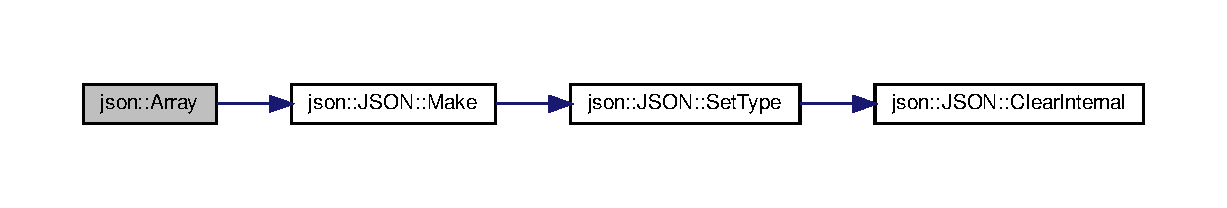
\includegraphics[width=350pt]{namespacejson_a805054691c80da00fd9129387f834c21_cgraph}
\end{center}
\end{figure}
Here is the caller graph for this function\+:
\nopagebreak
\begin{figure}[H]
\begin{center}
\leavevmode
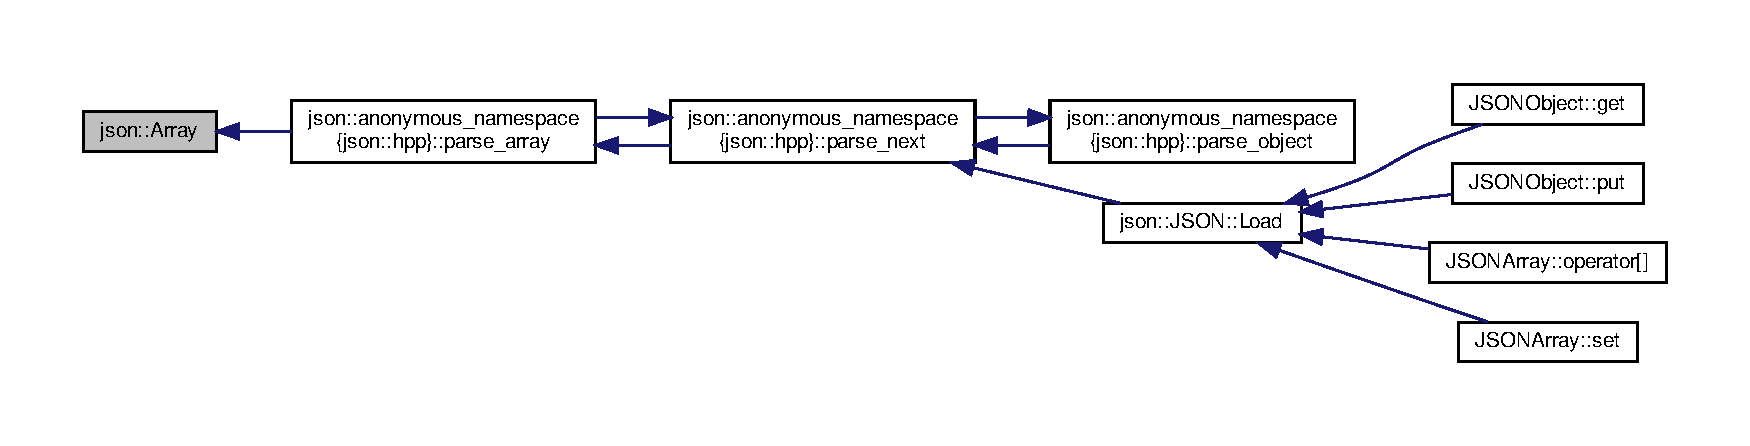
\includegraphics[width=350pt]{namespacejson_a805054691c80da00fd9129387f834c21_icgraph}
\end{center}
\end{figure}
\mbox{\Hypertarget{namespacejson_a8c39b1bf99577bc140f0647d0192219f}\label{namespacejson_a8c39b1bf99577bc140f0647d0192219f}} 
\index{json@{json}!Array@{Array}}
\index{Array@{Array}!json@{json}}
\subsubsection{\texorpdfstring{Array()}{Array()}\hspace{0.1cm}{\footnotesize\ttfamily [2/2]}}
{\footnotesize\ttfamily template$<$typename... T$>$ \\
\mbox{\hyperlink{classjson_1_1_j_s_o_n}{J\+S\+ON}} json\+::\+Array (\begin{DoxyParamCaption}\item[{T...}]{args }\end{DoxyParamCaption})}



Definition at line 426 of file json.\+hpp.



References json\+::\+J\+S\+O\+N\+::append(), json\+::\+J\+S\+O\+N\+::\+Array, and json\+::\+J\+S\+O\+N\+::\+Make().


\begin{DoxyCode}
426                         \{
427     \mbox{\hyperlink{class_j_s_o_n}{JSON}} arr = JSON::Make( \mbox{\hyperlink{namespacejson_a8c39b1bf99577bc140f0647d0192219f}{JSON::Class::Array}} );
428     arr.append( args... );
429     \textcolor{keywordflow}{return} std::move( arr );
430 \}
\end{DoxyCode}
Here is the call graph for this function\+:
\nopagebreak
\begin{figure}[H]
\begin{center}
\leavevmode
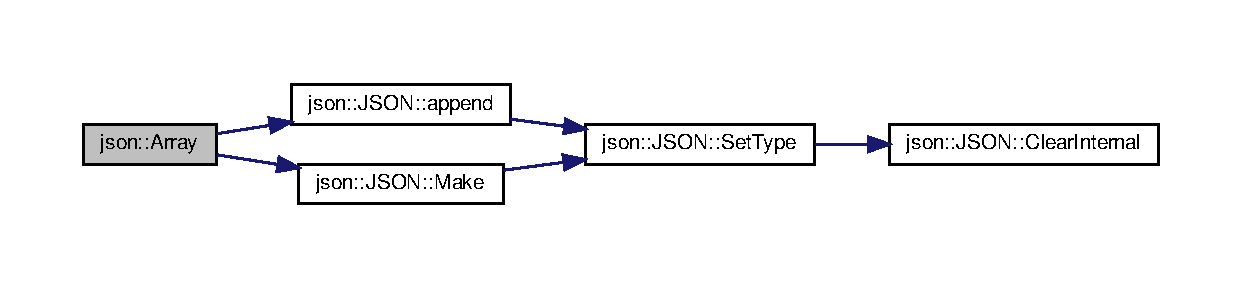
\includegraphics[width=350pt]{namespacejson_a8c39b1bf99577bc140f0647d0192219f_cgraph}
\end{center}
\end{figure}
\mbox{\Hypertarget{namespacejson_a7bc7d25f21c18a652a42db29cfdabd06}\label{namespacejson_a7bc7d25f21c18a652a42db29cfdabd06}} 
\index{json@{json}!Object@{Object}}
\index{Object@{Object}!json@{json}}
\subsubsection{\texorpdfstring{Object()}{Object()}}
{\footnotesize\ttfamily \mbox{\hyperlink{classjson_1_1_j_s_o_n}{J\+S\+ON}} json\+::\+Object (\begin{DoxyParamCaption}{ }\end{DoxyParamCaption})\hspace{0.3cm}{\ttfamily [inline]}}



Definition at line 432 of file json.\+hpp.



References json\+::\+J\+S\+O\+N\+::\+Make(), and json\+::\+J\+S\+O\+N\+::\+Object.



Referenced by json\+::anonymous\+\_\+namespace\{json.\+hpp\}\+::parse\+\_\+object().


\begin{DoxyCode}
432                      \{
433     \textcolor{keywordflow}{return} std::move( JSON::Make( \mbox{\hyperlink{namespacejson_a7bc7d25f21c18a652a42db29cfdabd06}{JSON::Class::Object}} ) );
434 \}
\end{DoxyCode}
Here is the call graph for this function\+:
\nopagebreak
\begin{figure}[H]
\begin{center}
\leavevmode
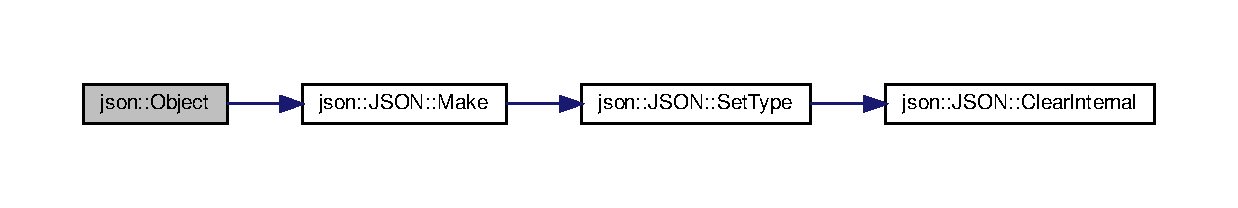
\includegraphics[width=350pt]{namespacejson_a7bc7d25f21c18a652a42db29cfdabd06_cgraph}
\end{center}
\end{figure}
Here is the caller graph for this function\+:
\nopagebreak
\begin{figure}[H]
\begin{center}
\leavevmode
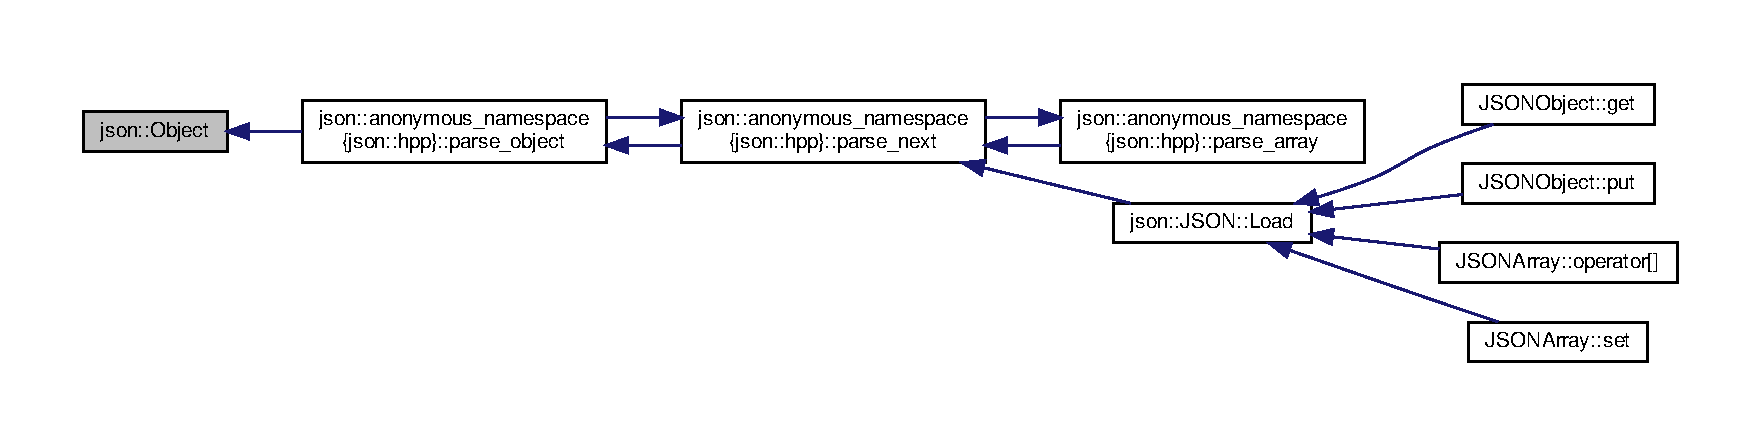
\includegraphics[width=350pt]{namespacejson_a7bc7d25f21c18a652a42db29cfdabd06_icgraph}
\end{center}
\end{figure}
\mbox{\Hypertarget{namespacejson_a348c2e5bffbeca243a52de2977e71b08}\label{namespacejson_a348c2e5bffbeca243a52de2977e71b08}} 
\index{json@{json}!operator$<$$<$@{operator$<$$<$}}
\index{operator$<$$<$@{operator$<$$<$}!json@{json}}
\subsubsection{\texorpdfstring{operator$<$$<$()}{operator<<()}}
{\footnotesize\ttfamily std\+::ostream\& json\+::operator$<$$<$ (\begin{DoxyParamCaption}\item[{std\+::ostream \&}]{os,  }\item[{const \mbox{\hyperlink{classjson_1_1_j_s_o_n}{J\+S\+ON}} \&}]{json }\end{DoxyParamCaption})\hspace{0.3cm}{\ttfamily [inline]}}



Definition at line 436 of file json.\+hpp.


\begin{DoxyCode}
436                                                                   \{
437     os << \mbox{\hyperlink{namespacejson}{json}}.dump();
438     \textcolor{keywordflow}{return} os;
439 \}
\end{DoxyCode}

\hypertarget{namespacejson_1_1anonymous__namespace_02json_8hpp_03}{}\section{json\+:\+:anonymous\+\_\+namespace\{json.\+hpp\} Namespace Reference}
\label{namespacejson_1_1anonymous__namespace_02json_8hpp_03}\index{json\+::anonymous\+\_\+namespace\lcurly{}json.\+hpp\rcurly{}@{json\+::anonymous\+\_\+namespace\lcurly{}json.\+hpp\rcurly{}}}
\subsection*{Functions}
\begin{DoxyCompactItemize}
\item 
string \mbox{\hyperlink{namespacejson_1_1anonymous__namespace_02json_8hpp_03_a623a6fca4cd1735d2bf3d081b875a350}{json\+\_\+escape}} (const string \&str)
\item 
\mbox{\hyperlink{classjson_1_1_j_s_o_n}{J\+S\+ON}} \mbox{\hyperlink{namespacejson_1_1anonymous__namespace_02json_8hpp_03_acd55b945d1583038db8633516df7cf3f}{parse\+\_\+next}} (const string \&, size\+\_\+t \&)
\item 
void \mbox{\hyperlink{namespacejson_1_1anonymous__namespace_02json_8hpp_03_a3a6e9a9e2d1cf7848055ae69f04be8b7}{consume\+\_\+ws}} (const string \&str, size\+\_\+t \&offset)
\item 
\mbox{\hyperlink{classjson_1_1_j_s_o_n}{J\+S\+ON}} \mbox{\hyperlink{namespacejson_1_1anonymous__namespace_02json_8hpp_03_a69b6c8f8bb93130f5c6dab832000f915}{parse\+\_\+object}} (const string \&str, size\+\_\+t \&offset)
\item 
\mbox{\hyperlink{classjson_1_1_j_s_o_n}{J\+S\+ON}} \mbox{\hyperlink{namespacejson_1_1anonymous__namespace_02json_8hpp_03_a6a3598f1545d6015c9db8015fc42f7ff}{parse\+\_\+array}} (const string \&str, size\+\_\+t \&offset)
\item 
\mbox{\hyperlink{classjson_1_1_j_s_o_n}{J\+S\+ON}} \mbox{\hyperlink{namespacejson_1_1anonymous__namespace_02json_8hpp_03_a274c7a1f9001093d6b093abb5481122b}{parse\+\_\+string}} (const string \&str, size\+\_\+t \&offset)
\item 
\mbox{\hyperlink{classjson_1_1_j_s_o_n}{J\+S\+ON}} \mbox{\hyperlink{namespacejson_1_1anonymous__namespace_02json_8hpp_03_a9cc81652562c9d3c0f639ce43057f09a}{parse\+\_\+number}} (const string \&str, size\+\_\+t \&offset)
\item 
\mbox{\hyperlink{classjson_1_1_j_s_o_n}{J\+S\+ON}} \mbox{\hyperlink{namespacejson_1_1anonymous__namespace_02json_8hpp_03_ae47f0a41d47e83e2ce1f5f267e938c1e}{parse\+\_\+bool}} (const string \&str, size\+\_\+t \&offset)
\item 
\mbox{\hyperlink{classjson_1_1_j_s_o_n}{J\+S\+ON}} \mbox{\hyperlink{namespacejson_1_1anonymous__namespace_02json_8hpp_03_ad65e6ea0d2d880b099cf399600bf5666}{parse\+\_\+null}} (const string \&str, size\+\_\+t \&offset)
\end{DoxyCompactItemize}


\subsection{Function Documentation}
\mbox{\Hypertarget{namespacejson_1_1anonymous__namespace_02json_8hpp_03_a3a6e9a9e2d1cf7848055ae69f04be8b7}\label{namespacejson_1_1anonymous__namespace_02json_8hpp_03_a3a6e9a9e2d1cf7848055ae69f04be8b7}} 
\index{json\+::anonymous\+\_\+namespace\lcurly{}json.\+hpp\rcurly{}@{json\+::anonymous\+\_\+namespace\lcurly{}json.\+hpp\rcurly{}}!consume\+\_\+ws@{consume\+\_\+ws}}
\index{consume\+\_\+ws@{consume\+\_\+ws}!json\+::anonymous\+\_\+namespace\lcurly{}json.\+hpp\rcurly{}@{json\+::anonymous\+\_\+namespace\lcurly{}json.\+hpp\rcurly{}}}
\subsubsection{\texorpdfstring{consume\+\_\+ws()}{consume\_ws()}}
{\footnotesize\ttfamily void json\+::anonymous\+\_\+namespace\{json.\+hpp\}\+::consume\+\_\+ws (\begin{DoxyParamCaption}\item[{const string \&}]{str,  }\item[{size\+\_\+t \&}]{offset }\end{DoxyParamCaption})}



Definition at line 444 of file json.\+hpp.



Referenced by parse\+\_\+array(), parse\+\_\+next(), and parse\+\_\+object().


\begin{DoxyCode}
444                                                          \{
445         \textcolor{keywordflow}{while}( isspace( str[offset] ) ) ++offset;
446     \}
\end{DoxyCode}
Here is the caller graph for this function\+:
\nopagebreak
\begin{figure}[H]
\begin{center}
\leavevmode
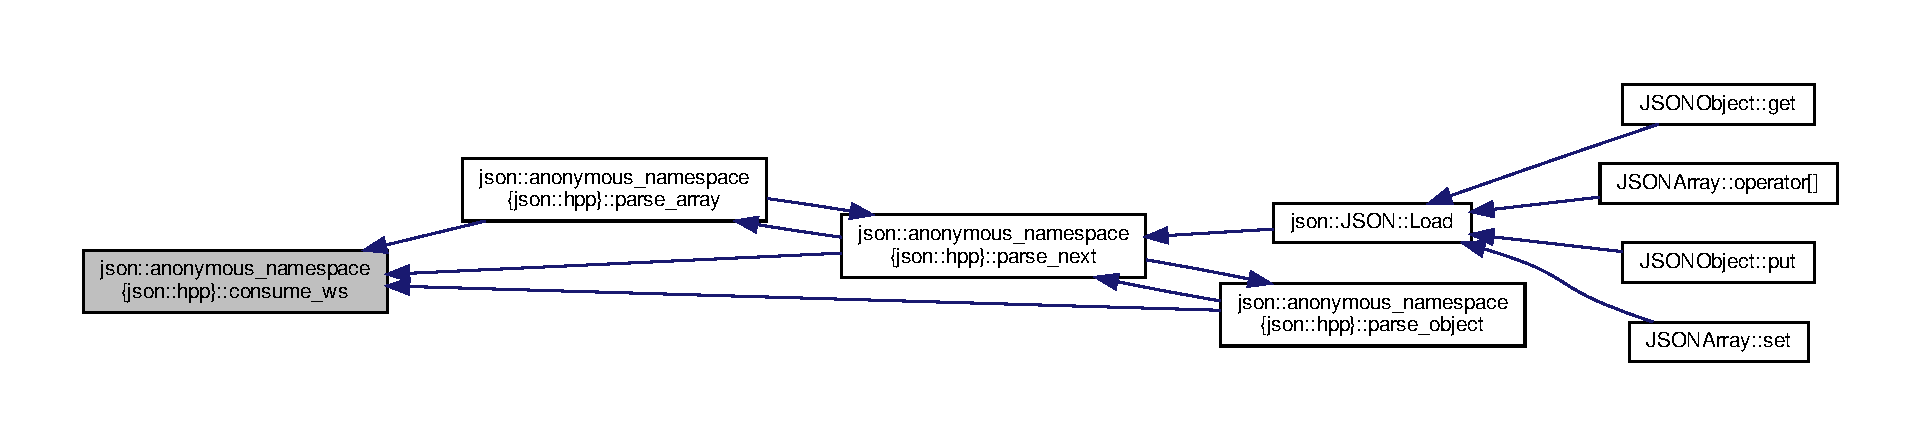
\includegraphics[width=350pt]{namespacejson_1_1anonymous__namespace_02json_8hpp_03_a3a6e9a9e2d1cf7848055ae69f04be8b7_icgraph}
\end{center}
\end{figure}
\mbox{\Hypertarget{namespacejson_1_1anonymous__namespace_02json_8hpp_03_a623a6fca4cd1735d2bf3d081b875a350}\label{namespacejson_1_1anonymous__namespace_02json_8hpp_03_a623a6fca4cd1735d2bf3d081b875a350}} 
\index{json\+::anonymous\+\_\+namespace\lcurly{}json.\+hpp\rcurly{}@{json\+::anonymous\+\_\+namespace\lcurly{}json.\+hpp\rcurly{}}!json\+\_\+escape@{json\+\_\+escape}}
\index{json\+\_\+escape@{json\+\_\+escape}!json\+::anonymous\+\_\+namespace\lcurly{}json.\+hpp\rcurly{}@{json\+::anonymous\+\_\+namespace\lcurly{}json.\+hpp\rcurly{}}}
\subsubsection{\texorpdfstring{json\+\_\+escape()}{json\_escape()}}
{\footnotesize\ttfamily string json\+::anonymous\+\_\+namespace\{json.\+hpp\}\+::json\+\_\+escape (\begin{DoxyParamCaption}\item[{const string \&}]{str }\end{DoxyParamCaption})}



Definition at line 28 of file json.\+hpp.



Referenced by json\+::\+J\+S\+O\+N\+::dump(), and json\+::\+J\+S\+O\+N\+::\+To\+String().


\begin{DoxyCode}
28                                             \{
29         \textcolor{keywordtype}{string} output;
30         \textcolor{keywordflow}{for}( \textcolor{keywordtype}{unsigned} i = 0; i < str.length(); ++i )
31             \textcolor{keywordflow}{switch}( str[i] ) \{
32                 \textcolor{keywordflow}{case} \textcolor{charliteral}{'\(\backslash\)"'}: output += \textcolor{stringliteral}{"\(\backslash\)\(\backslash\)\(\backslash\)""}; \textcolor{keywordflow}{break};
33                 \textcolor{keywordflow}{case} \textcolor{charliteral}{'\(\backslash\)\(\backslash\)'}: output += \textcolor{stringliteral}{"\(\backslash\)\(\backslash\)\(\backslash\)\(\backslash\)"}; \textcolor{keywordflow}{break};
34                 \textcolor{keywordflow}{case} \textcolor{charliteral}{'\(\backslash\)b'}: output += \textcolor{stringliteral}{"\(\backslash\)\(\backslash\)b"};  \textcolor{keywordflow}{break};
35                 \textcolor{keywordflow}{case} \textcolor{charliteral}{'\(\backslash\)f'}: output += \textcolor{stringliteral}{"\(\backslash\)\(\backslash\)f"};  \textcolor{keywordflow}{break};
36                 \textcolor{keywordflow}{case} \textcolor{charliteral}{'\(\backslash\)n'}: output += \textcolor{stringliteral}{"\(\backslash\)\(\backslash\)n"};  \textcolor{keywordflow}{break};
37                 \textcolor{keywordflow}{case} \textcolor{charliteral}{'\(\backslash\)r'}: output += \textcolor{stringliteral}{"\(\backslash\)\(\backslash\)r"};  \textcolor{keywordflow}{break};
38                 \textcolor{keywordflow}{case} \textcolor{charliteral}{'\(\backslash\)t'}: output += \textcolor{stringliteral}{"\(\backslash\)\(\backslash\)t"};  \textcolor{keywordflow}{break};
39                 default  : output += str[i]; \textcolor{keywordflow}{break};
40             \}
41         \textcolor{keywordflow}{return} std::move( output );
42     \}
\end{DoxyCode}
Here is the caller graph for this function\+:
\nopagebreak
\begin{figure}[H]
\begin{center}
\leavevmode
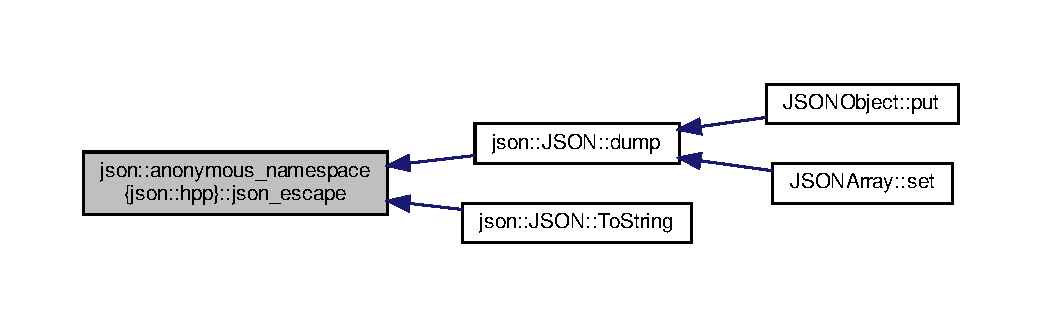
\includegraphics[width=350pt]{namespacejson_1_1anonymous__namespace_02json_8hpp_03_a623a6fca4cd1735d2bf3d081b875a350_icgraph}
\end{center}
\end{figure}
\mbox{\Hypertarget{namespacejson_1_1anonymous__namespace_02json_8hpp_03_a6a3598f1545d6015c9db8015fc42f7ff}\label{namespacejson_1_1anonymous__namespace_02json_8hpp_03_a6a3598f1545d6015c9db8015fc42f7ff}} 
\index{json\+::anonymous\+\_\+namespace\lcurly{}json.\+hpp\rcurly{}@{json\+::anonymous\+\_\+namespace\lcurly{}json.\+hpp\rcurly{}}!parse\+\_\+array@{parse\+\_\+array}}
\index{parse\+\_\+array@{parse\+\_\+array}!json\+::anonymous\+\_\+namespace\lcurly{}json.\+hpp\rcurly{}@{json\+::anonymous\+\_\+namespace\lcurly{}json.\+hpp\rcurly{}}}
\subsubsection{\texorpdfstring{parse\+\_\+array()}{parse\_array()}}
{\footnotesize\ttfamily \mbox{\hyperlink{classjson_1_1_j_s_o_n}{J\+S\+ON}} json\+::anonymous\+\_\+namespace\{json.\+hpp\}\+::parse\+\_\+array (\begin{DoxyParamCaption}\item[{const string \&}]{str,  }\item[{size\+\_\+t \&}]{offset }\end{DoxyParamCaption})}



Definition at line 484 of file json.\+hpp.



References json\+::\+J\+S\+O\+N\+::\+Array, json\+::\+Array(), consume\+\_\+ws(), json\+::\+J\+S\+O\+N\+::\+Make(), and parse\+\_\+next().



Referenced by parse\+\_\+next().


\begin{DoxyCode}
484                                                           \{
485         \mbox{\hyperlink{class_j_s_o_n}{JSON}} \mbox{\hyperlink{namespacejson_a8c39b1bf99577bc140f0647d0192219f}{Array}} = JSON::Make( \mbox{\hyperlink{namespacejson_a8c39b1bf99577bc140f0647d0192219f}{JSON::Class::Array}} );
486         \textcolor{keywordtype}{unsigned} index = 0;
487         
488         ++offset;
489         \mbox{\hyperlink{namespacejson_1_1anonymous__namespace_02json_8hpp_03_a3a6e9a9e2d1cf7848055ae69f04be8b7}{consume\_ws}}( str, offset );
490         \textcolor{keywordflow}{if}( str[offset] == \textcolor{charliteral}{']'} ) \{
491             ++offset; \textcolor{keywordflow}{return} std::move( \mbox{\hyperlink{namespacejson_a8c39b1bf99577bc140f0647d0192219f}{Array}} );
492         \}
493 
494         \textcolor{keywordflow}{while}( \textcolor{keyword}{true} ) \{
495             \mbox{\hyperlink{namespacejson_a8c39b1bf99577bc140f0647d0192219f}{Array}}[index++] = \mbox{\hyperlink{namespacejson_1_1anonymous__namespace_02json_8hpp_03_acd55b945d1583038db8633516df7cf3f}{parse\_next}}( str, offset );
496             \mbox{\hyperlink{namespacejson_1_1anonymous__namespace_02json_8hpp_03_a3a6e9a9e2d1cf7848055ae69f04be8b7}{consume\_ws}}( str, offset );
497 
498             \textcolor{keywordflow}{if}( str[offset] == \textcolor{charliteral}{','} ) \{
499                 ++offset; \textcolor{keywordflow}{continue};
500             \}
501             \textcolor{keywordflow}{else} \textcolor{keywordflow}{if}( str[offset] == \textcolor{charliteral}{']'} ) \{
502                 ++offset; \textcolor{keywordflow}{break};
503             \}
504             \textcolor{keywordflow}{else} \{
505                 std::cerr << \textcolor{stringliteral}{"ERROR: Array: Expected ',' or ']', found '"} << str[offset] << \textcolor{stringliteral}{"'\(\backslash\)n"};
506                 \textcolor{keywordflow}{return} std::move( JSON::Make( \mbox{\hyperlink{namespacejson_a8c39b1bf99577bc140f0647d0192219f}{JSON::Class::Array}} ) );
507             \}
508         \}
509 
510         \textcolor{keywordflow}{return} std::move( \mbox{\hyperlink{namespacejson_a8c39b1bf99577bc140f0647d0192219f}{Array}} );
511     \}
\end{DoxyCode}
Here is the call graph for this function\+:
\nopagebreak
\begin{figure}[H]
\begin{center}
\leavevmode
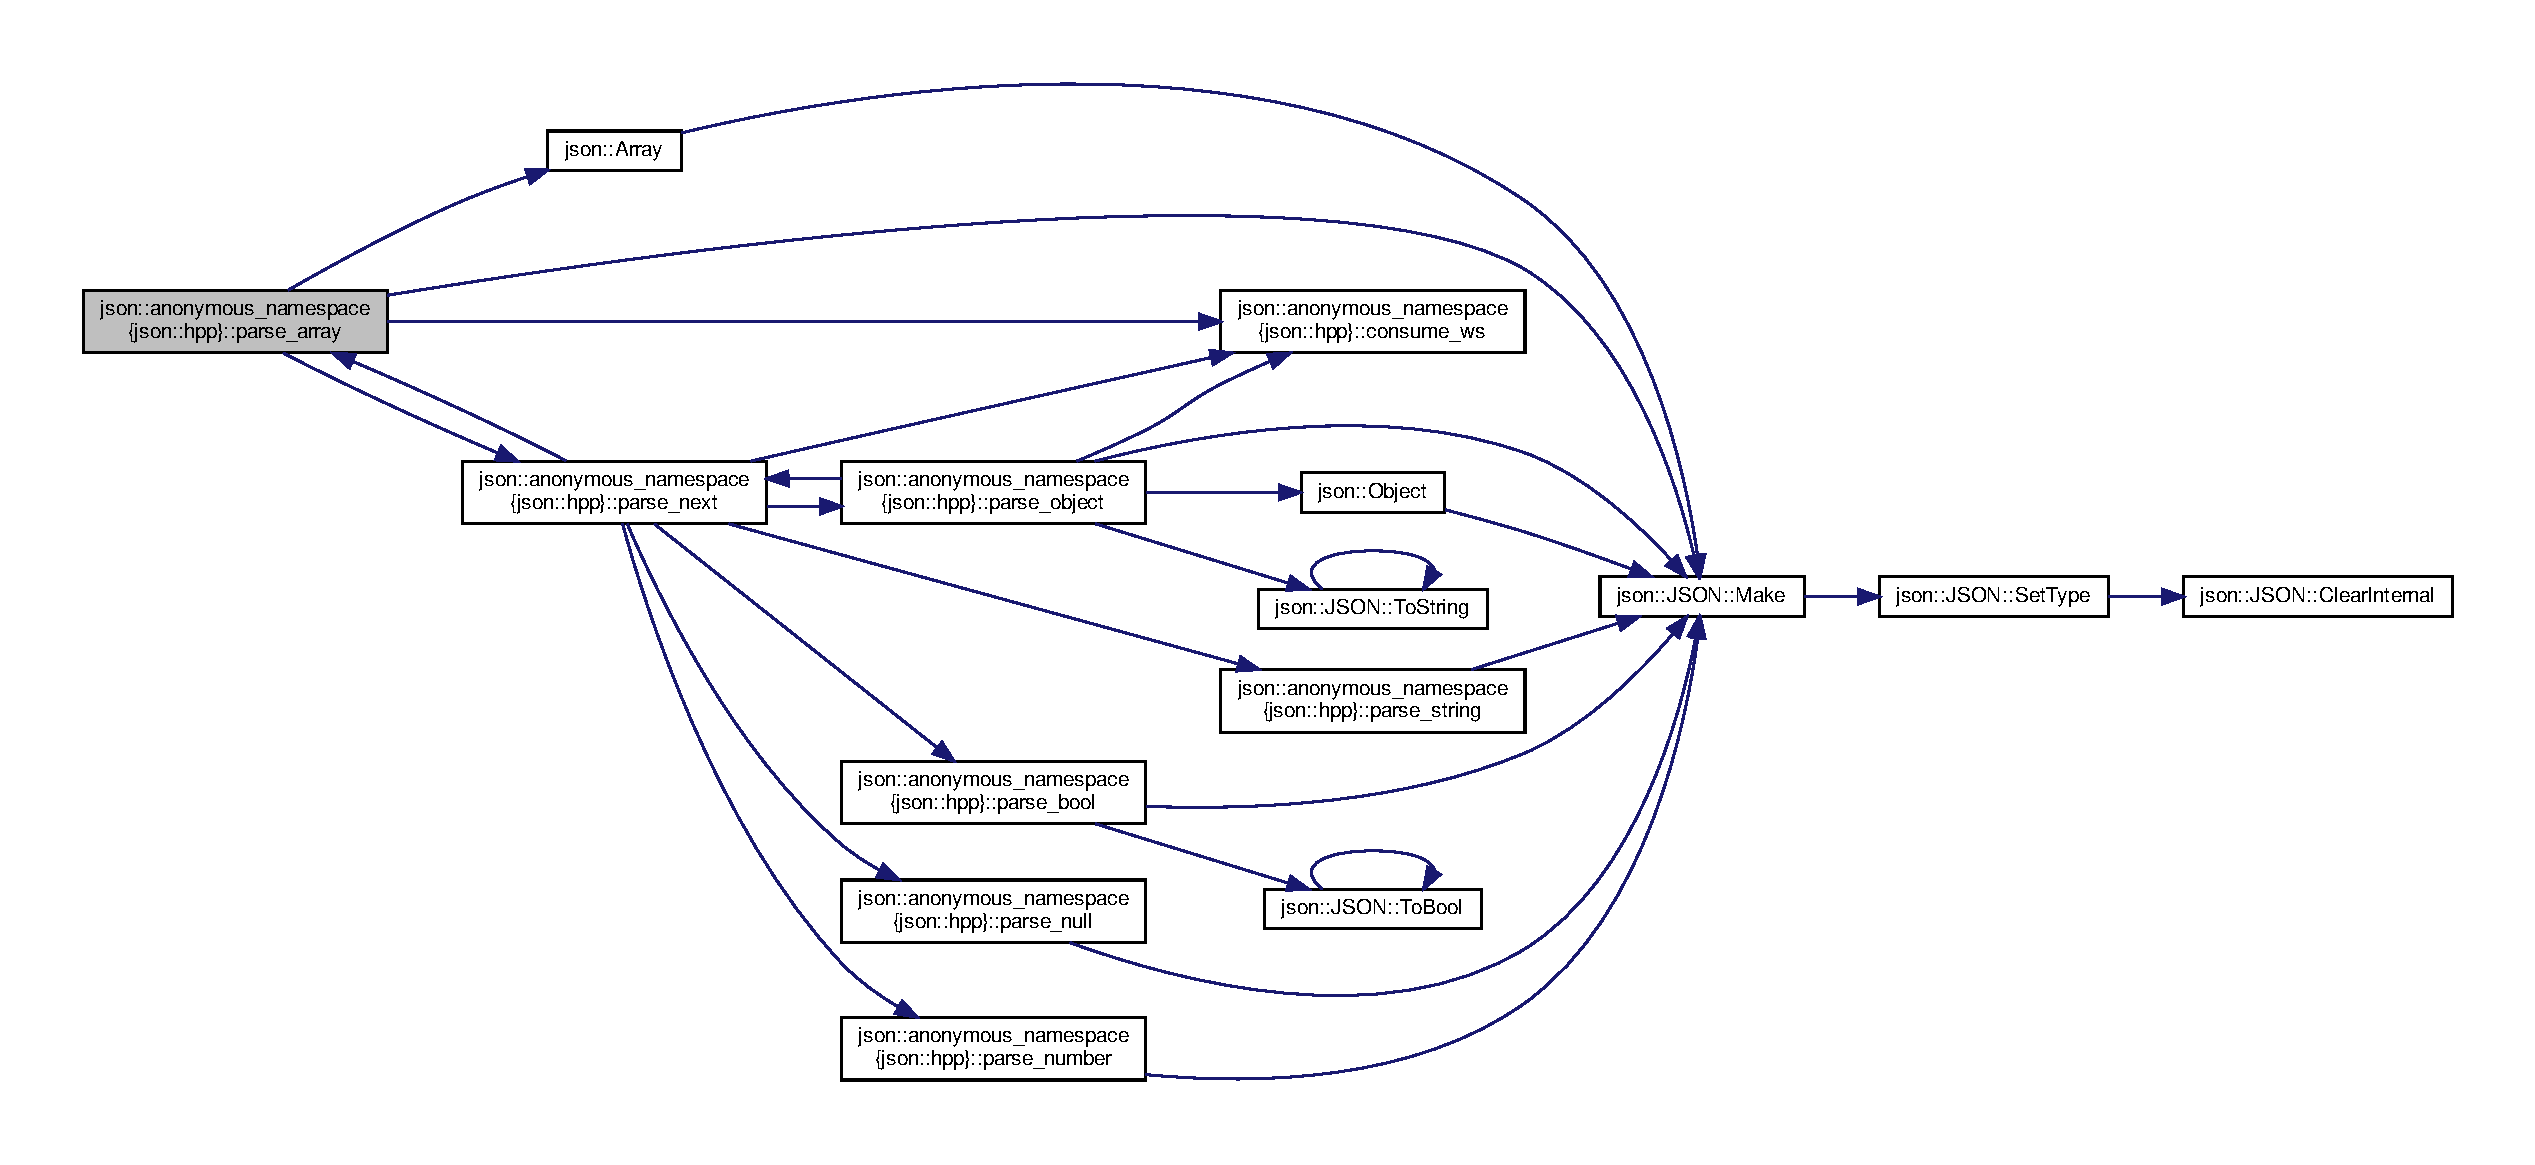
\includegraphics[width=350pt]{namespacejson_1_1anonymous__namespace_02json_8hpp_03_a6a3598f1545d6015c9db8015fc42f7ff_cgraph}
\end{center}
\end{figure}
Here is the caller graph for this function\+:
\nopagebreak
\begin{figure}[H]
\begin{center}
\leavevmode
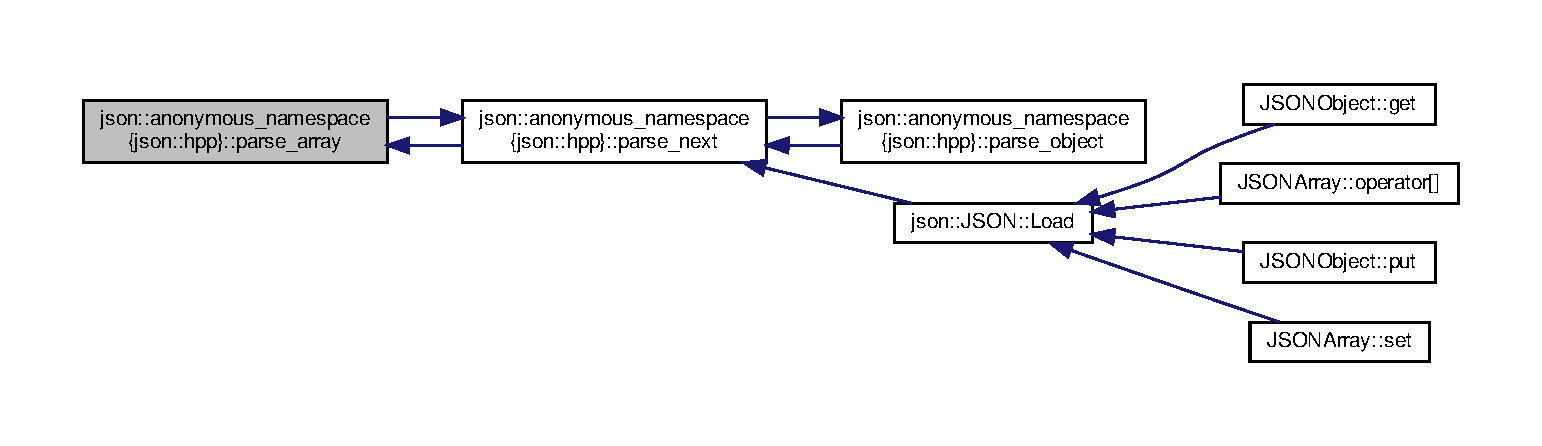
\includegraphics[width=350pt]{namespacejson_1_1anonymous__namespace_02json_8hpp_03_a6a3598f1545d6015c9db8015fc42f7ff_icgraph}
\end{center}
\end{figure}
\mbox{\Hypertarget{namespacejson_1_1anonymous__namespace_02json_8hpp_03_ae47f0a41d47e83e2ce1f5f267e938c1e}\label{namespacejson_1_1anonymous__namespace_02json_8hpp_03_ae47f0a41d47e83e2ce1f5f267e938c1e}} 
\index{json\+::anonymous\+\_\+namespace\lcurly{}json.\+hpp\rcurly{}@{json\+::anonymous\+\_\+namespace\lcurly{}json.\+hpp\rcurly{}}!parse\+\_\+bool@{parse\+\_\+bool}}
\index{parse\+\_\+bool@{parse\+\_\+bool}!json\+::anonymous\+\_\+namespace\lcurly{}json.\+hpp\rcurly{}@{json\+::anonymous\+\_\+namespace\lcurly{}json.\+hpp\rcurly{}}}
\subsubsection{\texorpdfstring{parse\+\_\+bool()}{parse\_bool()}}
{\footnotesize\ttfamily \mbox{\hyperlink{classjson_1_1_j_s_o_n}{J\+S\+ON}} json\+::anonymous\+\_\+namespace\{json.\+hpp\}\+::parse\+\_\+bool (\begin{DoxyParamCaption}\item[{const string \&}]{str,  }\item[{size\+\_\+t \&}]{offset }\end{DoxyParamCaption})}



Definition at line 601 of file json.\+hpp.



References json\+::\+J\+S\+O\+N\+::\+Make(), json\+::\+J\+S\+O\+N\+::\+Null, and json\+::\+J\+S\+O\+N\+::\+To\+Bool().



Referenced by parse\+\_\+next().


\begin{DoxyCode}
601                                                          \{
602         \mbox{\hyperlink{class_j_s_o_n}{JSON}} Bool;
603         \textcolor{keywordflow}{if}( str.substr( offset, 4 ) == \textcolor{stringliteral}{"true"} )
604             Bool = \textcolor{keyword}{true};
605         \textcolor{keywordflow}{else} \textcolor{keywordflow}{if}( str.substr( offset, 5 ) == \textcolor{stringliteral}{"false"} )
606             Bool = \textcolor{keyword}{false};
607         \textcolor{keywordflow}{else} \{
608             std::cerr << \textcolor{stringliteral}{"ERROR: Bool: Expected 'true' or 'false', found '"} << str.substr( offset, 5 ) << \textcolor{stringliteral}{"
      '\(\backslash\)n"};
609             \textcolor{keywordflow}{return} std::move( JSON::Make( JSON::Class::Null ) );
610         \}
611         offset += (Bool.ToBool() ? 4 : 5);
612         \textcolor{keywordflow}{return} std::move( Bool );
613     \}
\end{DoxyCode}
Here is the call graph for this function\+:
\nopagebreak
\begin{figure}[H]
\begin{center}
\leavevmode
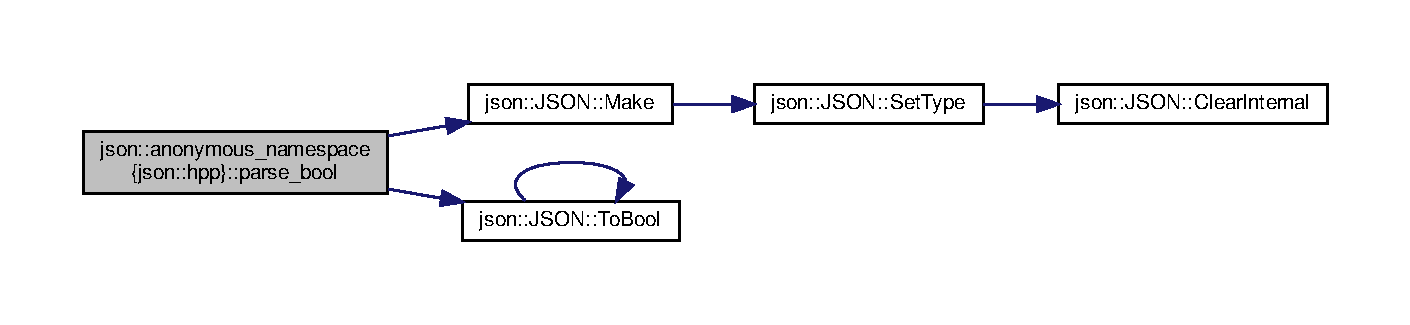
\includegraphics[width=350pt]{namespacejson_1_1anonymous__namespace_02json_8hpp_03_ae47f0a41d47e83e2ce1f5f267e938c1e_cgraph}
\end{center}
\end{figure}
Here is the caller graph for this function\+:
\nopagebreak
\begin{figure}[H]
\begin{center}
\leavevmode
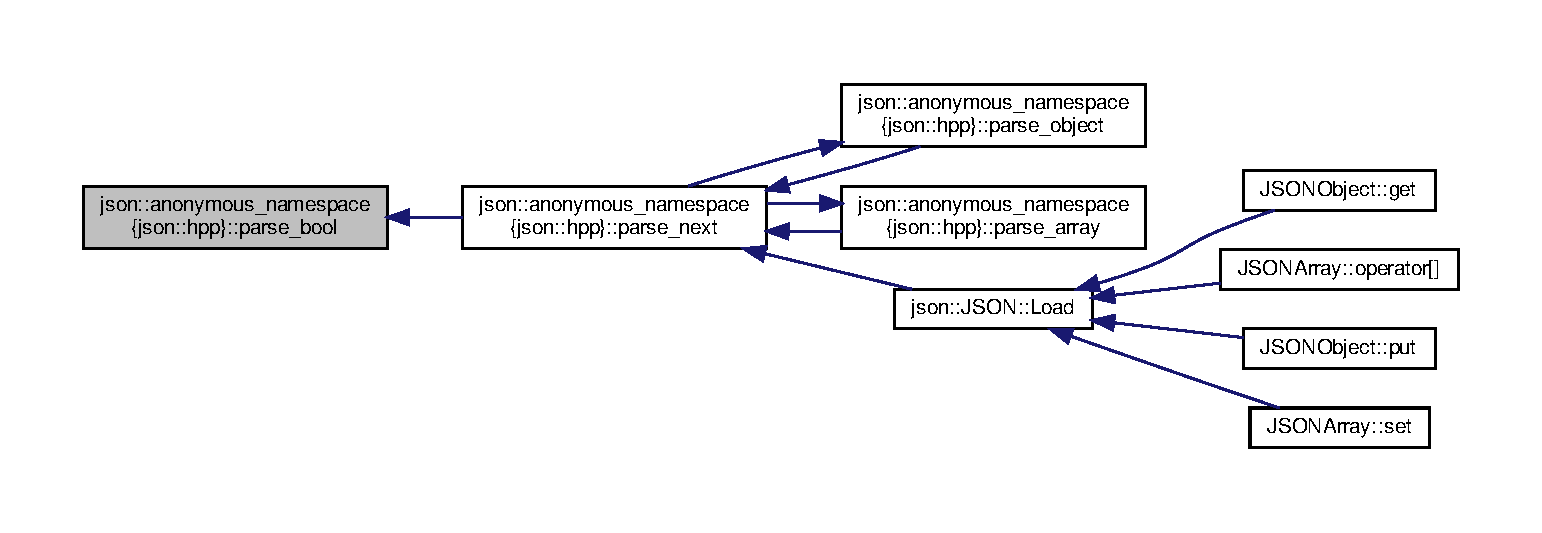
\includegraphics[width=350pt]{namespacejson_1_1anonymous__namespace_02json_8hpp_03_ae47f0a41d47e83e2ce1f5f267e938c1e_icgraph}
\end{center}
\end{figure}
\mbox{\Hypertarget{namespacejson_1_1anonymous__namespace_02json_8hpp_03_acd55b945d1583038db8633516df7cf3f}\label{namespacejson_1_1anonymous__namespace_02json_8hpp_03_acd55b945d1583038db8633516df7cf3f}} 
\index{json\+::anonymous\+\_\+namespace\lcurly{}json.\+hpp\rcurly{}@{json\+::anonymous\+\_\+namespace\lcurly{}json.\+hpp\rcurly{}}!parse\+\_\+next@{parse\+\_\+next}}
\index{parse\+\_\+next@{parse\+\_\+next}!json\+::anonymous\+\_\+namespace\lcurly{}json.\+hpp\rcurly{}@{json\+::anonymous\+\_\+namespace\lcurly{}json.\+hpp\rcurly{}}}
\subsubsection{\texorpdfstring{parse\+\_\+next()}{parse\_next()}}
{\footnotesize\ttfamily \mbox{\hyperlink{classjson_1_1_j_s_o_n}{J\+S\+ON}} json\+::anonymous\+\_\+namespace\{json.\+hpp\}\+::parse\+\_\+next (\begin{DoxyParamCaption}\item[{const string \&}]{str,  }\item[{size\+\_\+t \&}]{offset }\end{DoxyParamCaption})}



Definition at line 625 of file json.\+hpp.



References consume\+\_\+ws(), parse\+\_\+array(), parse\+\_\+bool(), parse\+\_\+null(), parse\+\_\+number(), parse\+\_\+object(), and parse\+\_\+string().



Referenced by json\+::\+J\+S\+O\+N\+::\+Load(), parse\+\_\+array(), and parse\+\_\+object().


\begin{DoxyCode}
625                                                          \{
626         \textcolor{keywordtype}{char} value;
627         \mbox{\hyperlink{namespacejson_1_1anonymous__namespace_02json_8hpp_03_a3a6e9a9e2d1cf7848055ae69f04be8b7}{consume\_ws}}( str, offset );
628         value = str[offset];
629         \textcolor{keywordflow}{switch}( value ) \{
630             \textcolor{keywordflow}{case} \textcolor{charliteral}{'['} : \textcolor{keywordflow}{return} std::move( \mbox{\hyperlink{namespacejson_1_1anonymous__namespace_02json_8hpp_03_a6a3598f1545d6015c9db8015fc42f7ff}{parse\_array}}( str, offset ) );
631             \textcolor{keywordflow}{case} \textcolor{charliteral}{'\{'} : \textcolor{keywordflow}{return} std::move( \mbox{\hyperlink{namespacejson_1_1anonymous__namespace_02json_8hpp_03_a69b6c8f8bb93130f5c6dab832000f915}{parse\_object}}( str, offset ) );
632             \textcolor{keywordflow}{case} \textcolor{charliteral}{'\(\backslash\)"'}: \textcolor{keywordflow}{return} std::move( \mbox{\hyperlink{namespacejson_1_1anonymous__namespace_02json_8hpp_03_a274c7a1f9001093d6b093abb5481122b}{parse\_string}}( str, offset ) );
633             \textcolor{keywordflow}{case} \textcolor{charliteral}{'t'} :
634             \textcolor{keywordflow}{case} \textcolor{charliteral}{'f'} : \textcolor{keywordflow}{return} std::move( \mbox{\hyperlink{namespacejson_1_1anonymous__namespace_02json_8hpp_03_ae47f0a41d47e83e2ce1f5f267e938c1e}{parse\_bool}}( str, offset ) );
635             \textcolor{keywordflow}{case} \textcolor{charliteral}{'n'} : \textcolor{keywordflow}{return} std::move( \mbox{\hyperlink{namespacejson_1_1anonymous__namespace_02json_8hpp_03_ad65e6ea0d2d880b099cf399600bf5666}{parse\_null}}( str, offset ) );
636             default  : \textcolor{keywordflow}{if}( ( value <= '9' && value >= \textcolor{charliteral}{'0'} ) || value == \textcolor{charliteral}{'-'} )
637                            \textcolor{keywordflow}{return} std::move( \mbox{\hyperlink{namespacejson_1_1anonymous__namespace_02json_8hpp_03_a9cc81652562c9d3c0f639ce43057f09a}{parse\_number}}( str, offset ) );
638         \}
639         std::cerr << \textcolor{stringliteral}{"ERROR: Parse: Unknown starting character '"} << value << \textcolor{stringliteral}{"'\(\backslash\)n"};
640         \textcolor{keywordflow}{return} \mbox{\hyperlink{class_j_s_o_n}{JSON}}();
641     \}
\end{DoxyCode}
Here is the call graph for this function\+:
\nopagebreak
\begin{figure}[H]
\begin{center}
\leavevmode
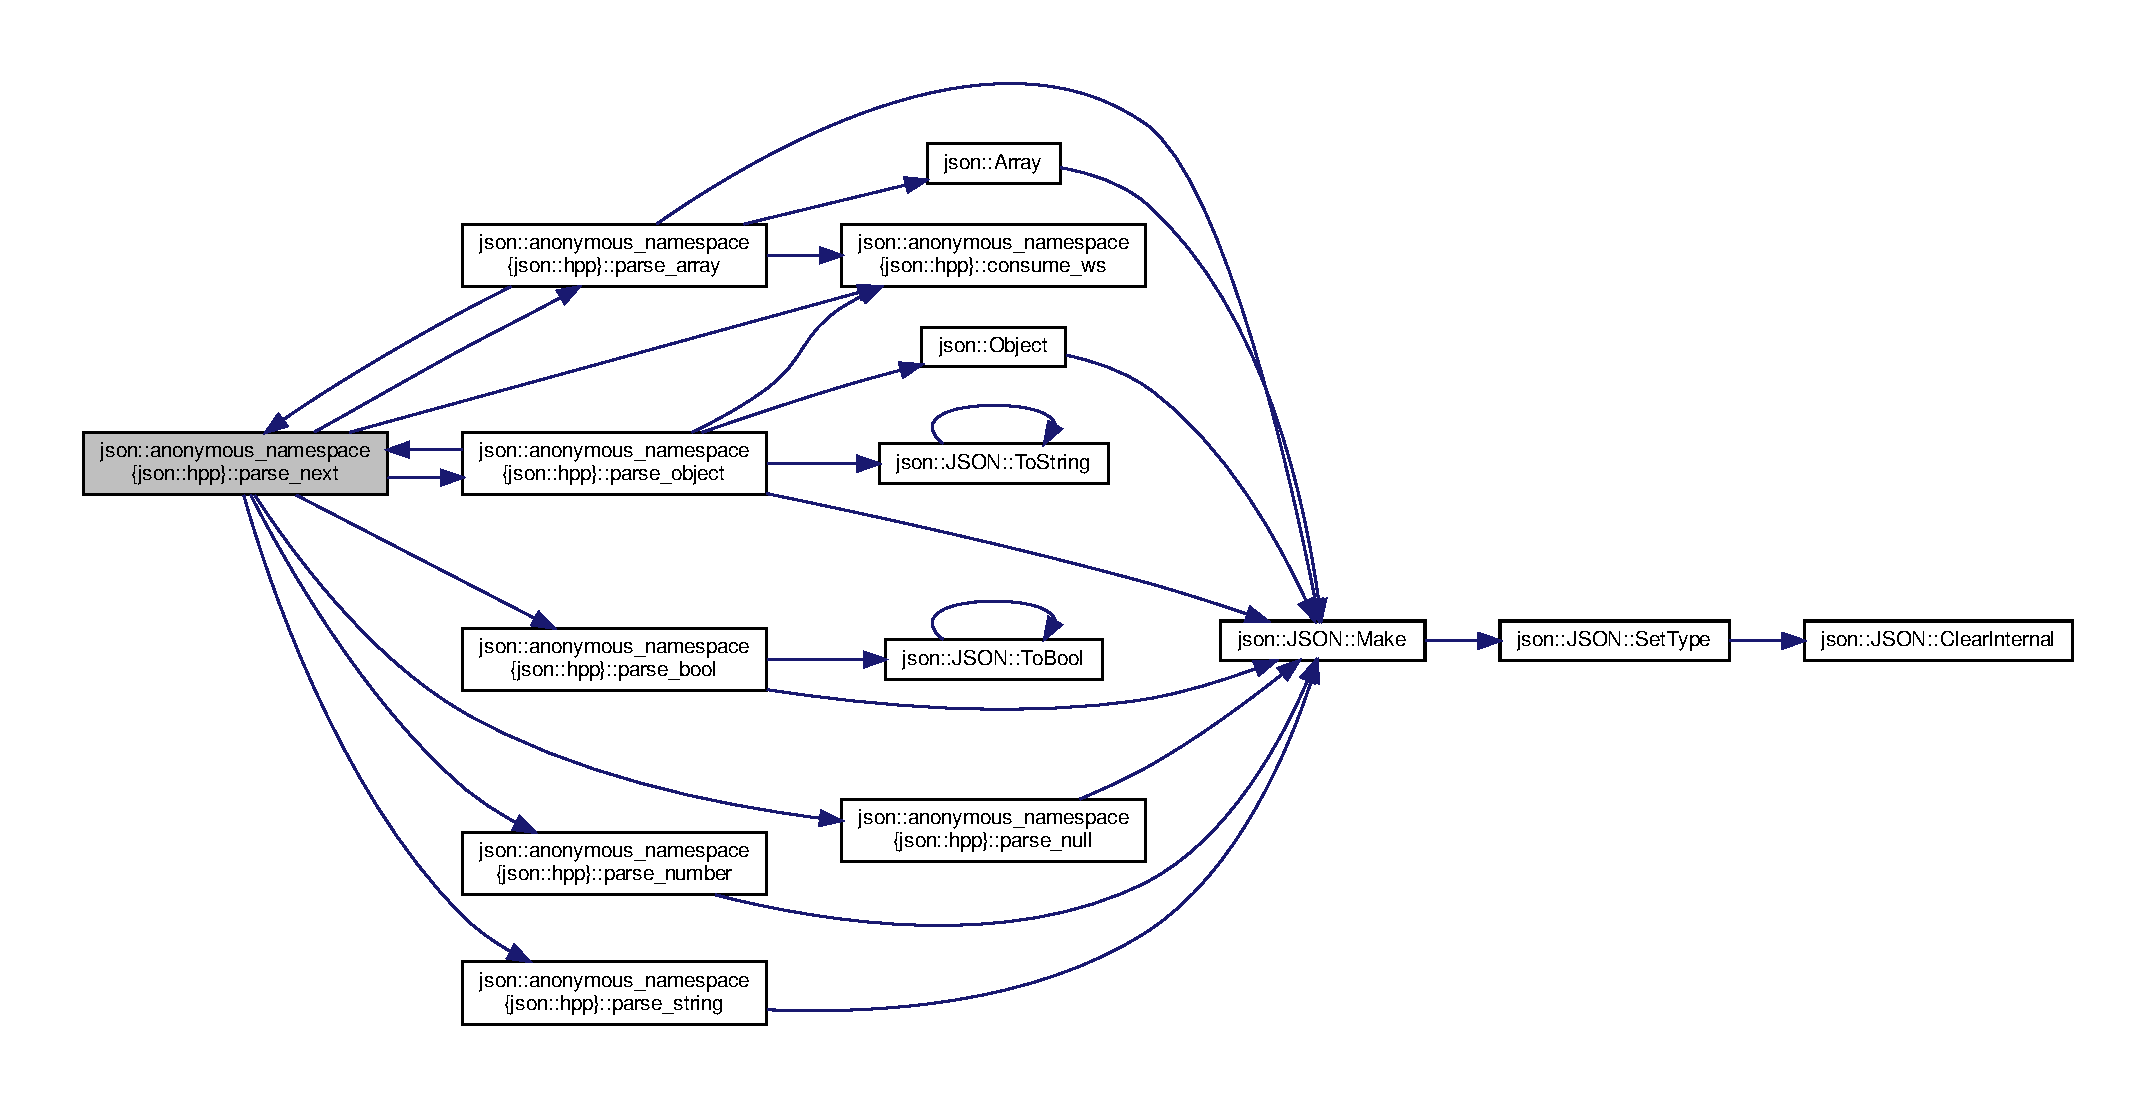
\includegraphics[width=350pt]{namespacejson_1_1anonymous__namespace_02json_8hpp_03_acd55b945d1583038db8633516df7cf3f_cgraph}
\end{center}
\end{figure}
Here is the caller graph for this function\+:
\nopagebreak
\begin{figure}[H]
\begin{center}
\leavevmode
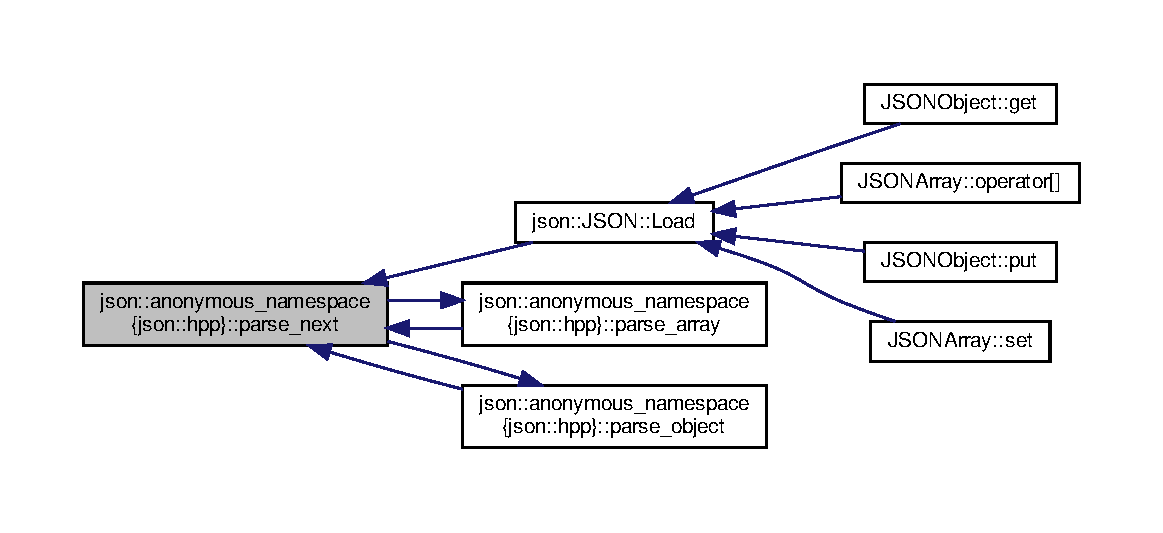
\includegraphics[width=350pt]{namespacejson_1_1anonymous__namespace_02json_8hpp_03_acd55b945d1583038db8633516df7cf3f_icgraph}
\end{center}
\end{figure}
\mbox{\Hypertarget{namespacejson_1_1anonymous__namespace_02json_8hpp_03_ad65e6ea0d2d880b099cf399600bf5666}\label{namespacejson_1_1anonymous__namespace_02json_8hpp_03_ad65e6ea0d2d880b099cf399600bf5666}} 
\index{json\+::anonymous\+\_\+namespace\lcurly{}json.\+hpp\rcurly{}@{json\+::anonymous\+\_\+namespace\lcurly{}json.\+hpp\rcurly{}}!parse\+\_\+null@{parse\+\_\+null}}
\index{parse\+\_\+null@{parse\+\_\+null}!json\+::anonymous\+\_\+namespace\lcurly{}json.\+hpp\rcurly{}@{json\+::anonymous\+\_\+namespace\lcurly{}json.\+hpp\rcurly{}}}
\subsubsection{\texorpdfstring{parse\+\_\+null()}{parse\_null()}}
{\footnotesize\ttfamily \mbox{\hyperlink{classjson_1_1_j_s_o_n}{J\+S\+ON}} json\+::anonymous\+\_\+namespace\{json.\+hpp\}\+::parse\+\_\+null (\begin{DoxyParamCaption}\item[{const string \&}]{str,  }\item[{size\+\_\+t \&}]{offset }\end{DoxyParamCaption})}



Definition at line 615 of file json.\+hpp.



References json\+::\+J\+S\+O\+N\+::\+Make(), and json\+::\+J\+S\+O\+N\+::\+Null.



Referenced by parse\+\_\+next().


\begin{DoxyCode}
615                                                          \{
616         \mbox{\hyperlink{class_j_s_o_n}{JSON}} Null;
617         \textcolor{keywordflow}{if}( str.substr( offset, 4 ) != \textcolor{stringliteral}{"null"} ) \{
618             std::cerr << \textcolor{stringliteral}{"ERROR: Null: Expected 'null', found '"} << str.substr( offset, 4 ) << \textcolor{stringliteral}{"'\(\backslash\)n"};
619             \textcolor{keywordflow}{return} std::move( JSON::Make( JSON::Class::Null ) );
620         \}
621         offset += 4;
622         \textcolor{keywordflow}{return} std::move( Null );
623     \}
\end{DoxyCode}
Here is the call graph for this function\+:
\nopagebreak
\begin{figure}[H]
\begin{center}
\leavevmode
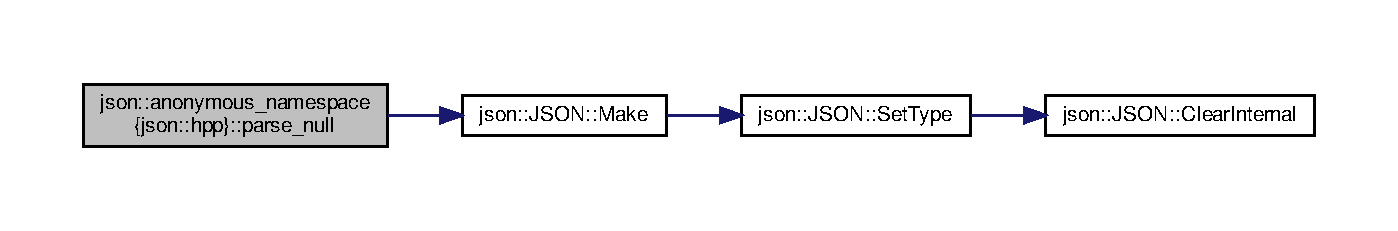
\includegraphics[width=350pt]{namespacejson_1_1anonymous__namespace_02json_8hpp_03_ad65e6ea0d2d880b099cf399600bf5666_cgraph}
\end{center}
\end{figure}
Here is the caller graph for this function\+:
\nopagebreak
\begin{figure}[H]
\begin{center}
\leavevmode
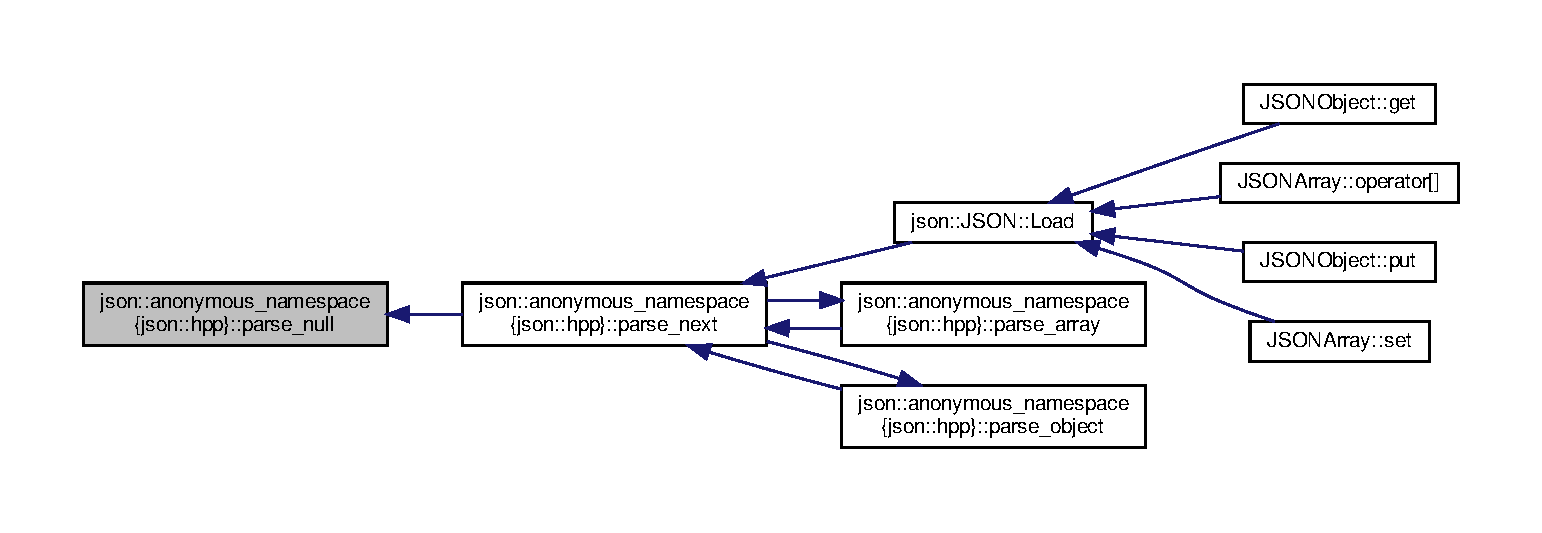
\includegraphics[width=350pt]{namespacejson_1_1anonymous__namespace_02json_8hpp_03_ad65e6ea0d2d880b099cf399600bf5666_icgraph}
\end{center}
\end{figure}
\mbox{\Hypertarget{namespacejson_1_1anonymous__namespace_02json_8hpp_03_a9cc81652562c9d3c0f639ce43057f09a}\label{namespacejson_1_1anonymous__namespace_02json_8hpp_03_a9cc81652562c9d3c0f639ce43057f09a}} 
\index{json\+::anonymous\+\_\+namespace\lcurly{}json.\+hpp\rcurly{}@{json\+::anonymous\+\_\+namespace\lcurly{}json.\+hpp\rcurly{}}!parse\+\_\+number@{parse\+\_\+number}}
\index{parse\+\_\+number@{parse\+\_\+number}!json\+::anonymous\+\_\+namespace\lcurly{}json.\+hpp\rcurly{}@{json\+::anonymous\+\_\+namespace\lcurly{}json.\+hpp\rcurly{}}}
\subsubsection{\texorpdfstring{parse\+\_\+number()}{parse\_number()}}
{\footnotesize\ttfamily \mbox{\hyperlink{classjson_1_1_j_s_o_n}{J\+S\+ON}} json\+::anonymous\+\_\+namespace\{json.\+hpp\}\+::parse\+\_\+number (\begin{DoxyParamCaption}\item[{const string \&}]{str,  }\item[{size\+\_\+t \&}]{offset }\end{DoxyParamCaption})}



Definition at line 551 of file json.\+hpp.



References json\+::\+J\+S\+O\+N\+::\+Make(), and json\+::\+J\+S\+O\+N\+::\+Null.



Referenced by parse\+\_\+next().


\begin{DoxyCode}
551                                                            \{
552         \mbox{\hyperlink{class_j_s_o_n}{JSON}} Number;
553         \textcolor{keywordtype}{string} val, exp\_str;
554         \textcolor{keywordtype}{char} c;
555         \textcolor{keywordtype}{bool} isDouble = \textcolor{keyword}{false};
556         \textcolor{keywordtype}{long} exp = 0;
557         \textcolor{keywordflow}{while}( \textcolor{keyword}{true} ) \{
558             c = str[offset++];
559             \textcolor{keywordflow}{if}( (c == \textcolor{charliteral}{'-'}) || (c >= \textcolor{charliteral}{'0'} && c <= \textcolor{charliteral}{'9'}) )
560                 val += c;
561             \textcolor{keywordflow}{else} \textcolor{keywordflow}{if}( c == \textcolor{charliteral}{'.'} ) \{
562                 val += c; 
563                 isDouble = \textcolor{keyword}{true};
564             \}
565             \textcolor{keywordflow}{else}
566                 \textcolor{keywordflow}{break};
567         \}
568         \textcolor{keywordflow}{if}( c == \textcolor{charliteral}{'E'} || c == \textcolor{charliteral}{'e'} ) \{
569             c = str[ offset++ ];
570             \textcolor{keywordflow}{if}( c == \textcolor{charliteral}{'-'} )\{ ++offset; exp\_str += \textcolor{charliteral}{'-'};\}
571             \textcolor{keywordflow}{while}( \textcolor{keyword}{true} ) \{
572                 c = str[ offset++ ];
573                 \textcolor{keywordflow}{if}( c >= \textcolor{charliteral}{'0'} && c <= \textcolor{charliteral}{'9'} )
574                     exp\_str += c;
575                 \textcolor{keywordflow}{else} \textcolor{keywordflow}{if}( !isspace( c ) && c != \textcolor{charliteral}{','} && c != \textcolor{charliteral}{']'} && c != \textcolor{charliteral}{'\}'} ) \{
576                     std::cerr << \textcolor{stringliteral}{"ERROR: Number: Expected a number for exponent, found '"} << c << \textcolor{stringliteral}{"'\(\backslash\)n"};
577                     \textcolor{keywordflow}{return} std::move( JSON::Make( JSON::Class::Null ) );
578                 \}
579                 \textcolor{keywordflow}{else}
580                     \textcolor{keywordflow}{break};
581             \}
582             exp = std::stol( exp\_str );
583         \}
584         \textcolor{keywordflow}{else} \textcolor{keywordflow}{if}( !isspace( c ) && c != \textcolor{charliteral}{','} && c != \textcolor{charliteral}{']'} && c != \textcolor{charliteral}{'\}'} ) \{
585             std::cerr << \textcolor{stringliteral}{"ERROR: Number: unexpected character '"} << c << \textcolor{stringliteral}{"'\(\backslash\)n"};
586             \textcolor{keywordflow}{return} std::move( JSON::Make( JSON::Class::Null ) );
587         \}
588         --offset;
589         
590         \textcolor{keywordflow}{if}( isDouble )
591             Number = std::stod( val ) * std::pow( 10, exp );
592         \textcolor{keywordflow}{else} \{
593             \textcolor{keywordflow}{if}( !exp\_str.empty() )
594                 Number = std::stol( val ) * std::pow( 10, exp );
595             \textcolor{keywordflow}{else}
596                 Number = std::stol( val );
597         \}
598         \textcolor{keywordflow}{return} std::move( Number );
599     \}
\end{DoxyCode}
Here is the call graph for this function\+:
\nopagebreak
\begin{figure}[H]
\begin{center}
\leavevmode
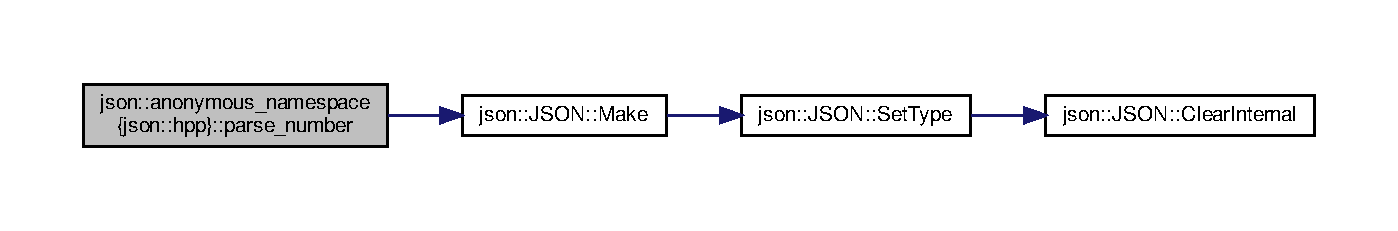
\includegraphics[width=350pt]{namespacejson_1_1anonymous__namespace_02json_8hpp_03_a9cc81652562c9d3c0f639ce43057f09a_cgraph}
\end{center}
\end{figure}
Here is the caller graph for this function\+:
\nopagebreak
\begin{figure}[H]
\begin{center}
\leavevmode
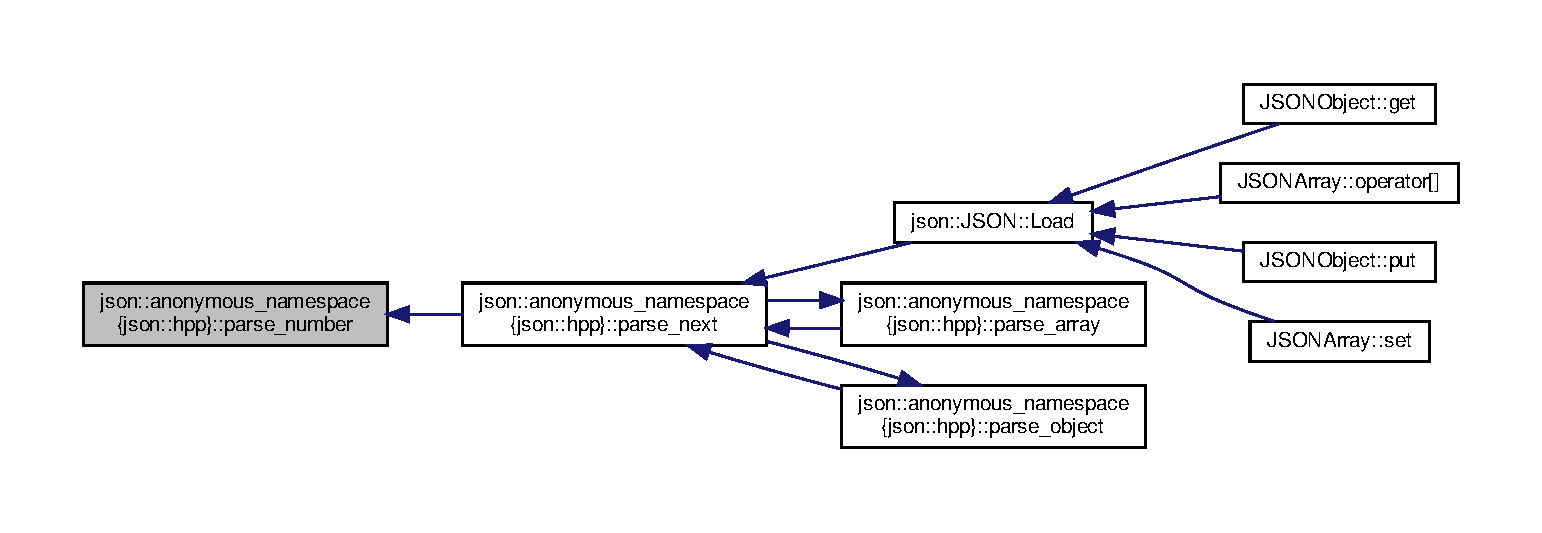
\includegraphics[width=350pt]{namespacejson_1_1anonymous__namespace_02json_8hpp_03_a9cc81652562c9d3c0f639ce43057f09a_icgraph}
\end{center}
\end{figure}
\mbox{\Hypertarget{namespacejson_1_1anonymous__namespace_02json_8hpp_03_a69b6c8f8bb93130f5c6dab832000f915}\label{namespacejson_1_1anonymous__namespace_02json_8hpp_03_a69b6c8f8bb93130f5c6dab832000f915}} 
\index{json\+::anonymous\+\_\+namespace\lcurly{}json.\+hpp\rcurly{}@{json\+::anonymous\+\_\+namespace\lcurly{}json.\+hpp\rcurly{}}!parse\+\_\+object@{parse\+\_\+object}}
\index{parse\+\_\+object@{parse\+\_\+object}!json\+::anonymous\+\_\+namespace\lcurly{}json.\+hpp\rcurly{}@{json\+::anonymous\+\_\+namespace\lcurly{}json.\+hpp\rcurly{}}}
\subsubsection{\texorpdfstring{parse\+\_\+object()}{parse\_object()}}
{\footnotesize\ttfamily \mbox{\hyperlink{classjson_1_1_j_s_o_n}{J\+S\+ON}} json\+::anonymous\+\_\+namespace\{json.\+hpp\}\+::parse\+\_\+object (\begin{DoxyParamCaption}\item[{const string \&}]{str,  }\item[{size\+\_\+t \&}]{offset }\end{DoxyParamCaption})}



Definition at line 448 of file json.\+hpp.



References consume\+\_\+ws(), json\+::\+J\+S\+O\+N\+::\+Make(), json\+::\+J\+S\+O\+N\+::\+Object, json\+::\+Object(), parse\+\_\+next(), and json\+::\+J\+S\+O\+N\+::\+To\+String().



Referenced by parse\+\_\+next().


\begin{DoxyCode}
448                                                            \{
449         \mbox{\hyperlink{class_j_s_o_n}{JSON}} \mbox{\hyperlink{namespacejson_a7bc7d25f21c18a652a42db29cfdabd06}{Object}} = JSON::Make( \mbox{\hyperlink{namespacejson_a7bc7d25f21c18a652a42db29cfdabd06}{JSON::Class::Object}} );
450 
451         ++offset;
452         \mbox{\hyperlink{namespacejson_1_1anonymous__namespace_02json_8hpp_03_a3a6e9a9e2d1cf7848055ae69f04be8b7}{consume\_ws}}( str, offset );
453         \textcolor{keywordflow}{if}( str[offset] == \textcolor{charliteral}{'\}'} ) \{
454             ++offset; \textcolor{keywordflow}{return} std::move( \mbox{\hyperlink{namespacejson_a7bc7d25f21c18a652a42db29cfdabd06}{Object}} );
455         \}
456 
457         \textcolor{keywordflow}{while}( \textcolor{keyword}{true} ) \{
458             \mbox{\hyperlink{class_j_s_o_n}{JSON}} Key = \mbox{\hyperlink{namespacejson_1_1anonymous__namespace_02json_8hpp_03_acd55b945d1583038db8633516df7cf3f}{parse\_next}}( str, offset );
459             \mbox{\hyperlink{namespacejson_1_1anonymous__namespace_02json_8hpp_03_a3a6e9a9e2d1cf7848055ae69f04be8b7}{consume\_ws}}( str, offset );
460             \textcolor{keywordflow}{if}( str[offset] != \textcolor{charliteral}{':'} ) \{
461                 std::cerr << \textcolor{stringliteral}{"Error: Object: Expected colon, found '"} << str[offset] << \textcolor{stringliteral}{"'\(\backslash\)n"};
462                 \textcolor{keywordflow}{break};
463             \}
464             \mbox{\hyperlink{namespacejson_1_1anonymous__namespace_02json_8hpp_03_a3a6e9a9e2d1cf7848055ae69f04be8b7}{consume\_ws}}( str, ++offset );
465             \mbox{\hyperlink{class_j_s_o_n}{JSON}} Value = \mbox{\hyperlink{namespacejson_1_1anonymous__namespace_02json_8hpp_03_acd55b945d1583038db8633516df7cf3f}{parse\_next}}( str, offset );
466             \mbox{\hyperlink{namespacejson_a7bc7d25f21c18a652a42db29cfdabd06}{Object}}[Key.ToString()] = Value;
467             
468             \mbox{\hyperlink{namespacejson_1_1anonymous__namespace_02json_8hpp_03_a3a6e9a9e2d1cf7848055ae69f04be8b7}{consume\_ws}}( str, offset );
469             \textcolor{keywordflow}{if}( str[offset] == \textcolor{charliteral}{','} ) \{
470                 ++offset; \textcolor{keywordflow}{continue};
471             \}
472             \textcolor{keywordflow}{else} \textcolor{keywordflow}{if}( str[offset] == \textcolor{charliteral}{'\}'} ) \{
473                 ++offset; \textcolor{keywordflow}{break};
474             \}
475             \textcolor{keywordflow}{else} \{
476                 std::cerr << \textcolor{stringliteral}{"ERROR: Object: Expected comma, found '"} << str[offset] << \textcolor{stringliteral}{"'\(\backslash\)n"};
477                 \textcolor{keywordflow}{break};
478             \}
479         \}
480 
481         \textcolor{keywordflow}{return} std::move( \mbox{\hyperlink{namespacejson_a7bc7d25f21c18a652a42db29cfdabd06}{Object}} );
482     \}
\end{DoxyCode}
Here is the call graph for this function\+:
\nopagebreak
\begin{figure}[H]
\begin{center}
\leavevmode
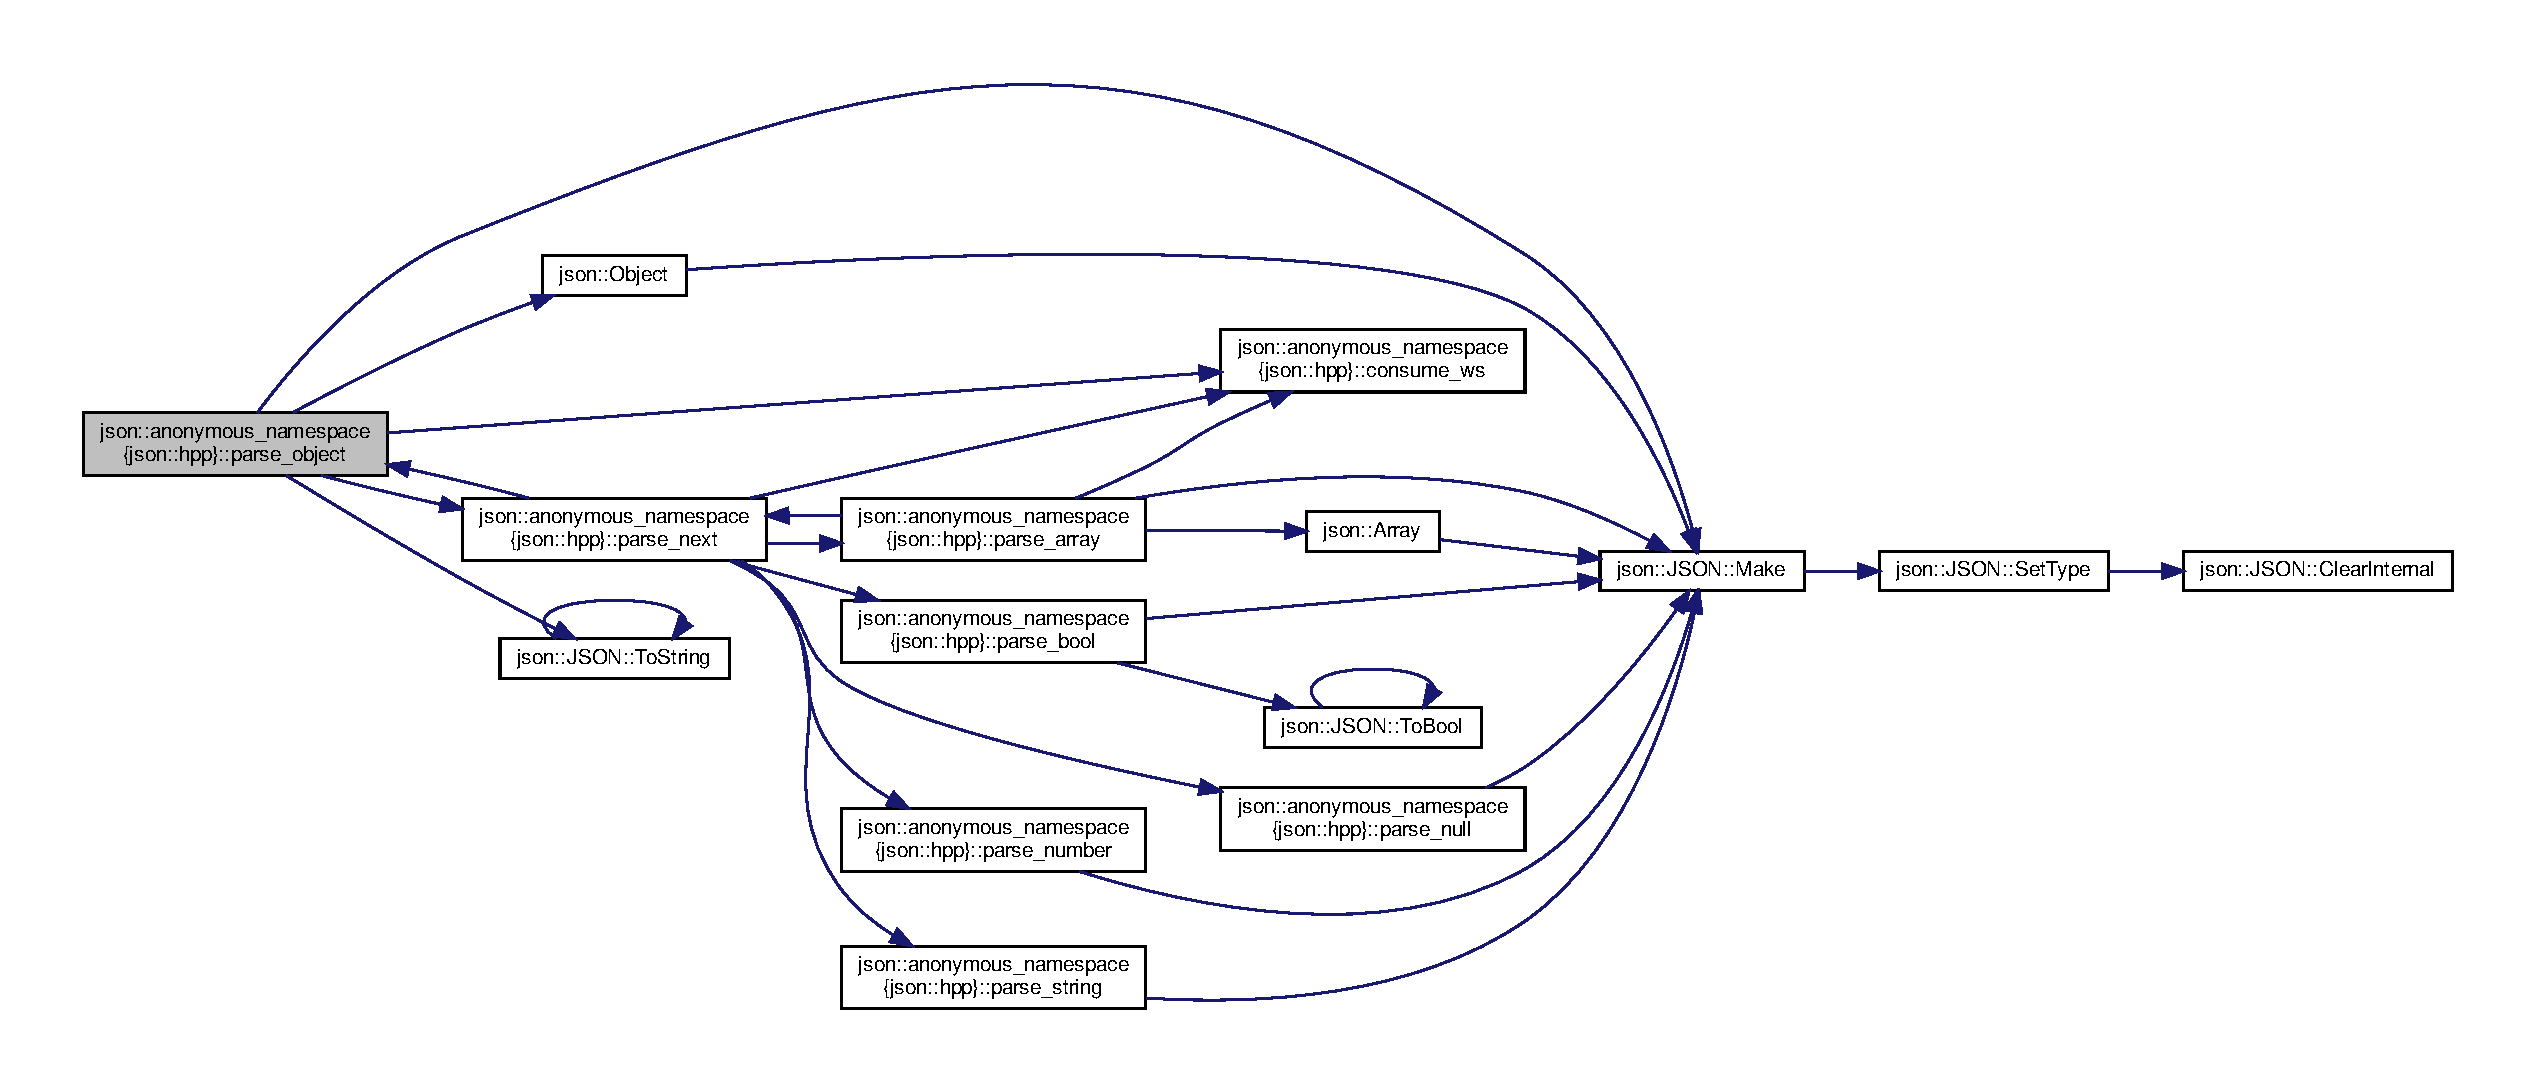
\includegraphics[width=350pt]{namespacejson_1_1anonymous__namespace_02json_8hpp_03_a69b6c8f8bb93130f5c6dab832000f915_cgraph}
\end{center}
\end{figure}
Here is the caller graph for this function\+:
\nopagebreak
\begin{figure}[H]
\begin{center}
\leavevmode
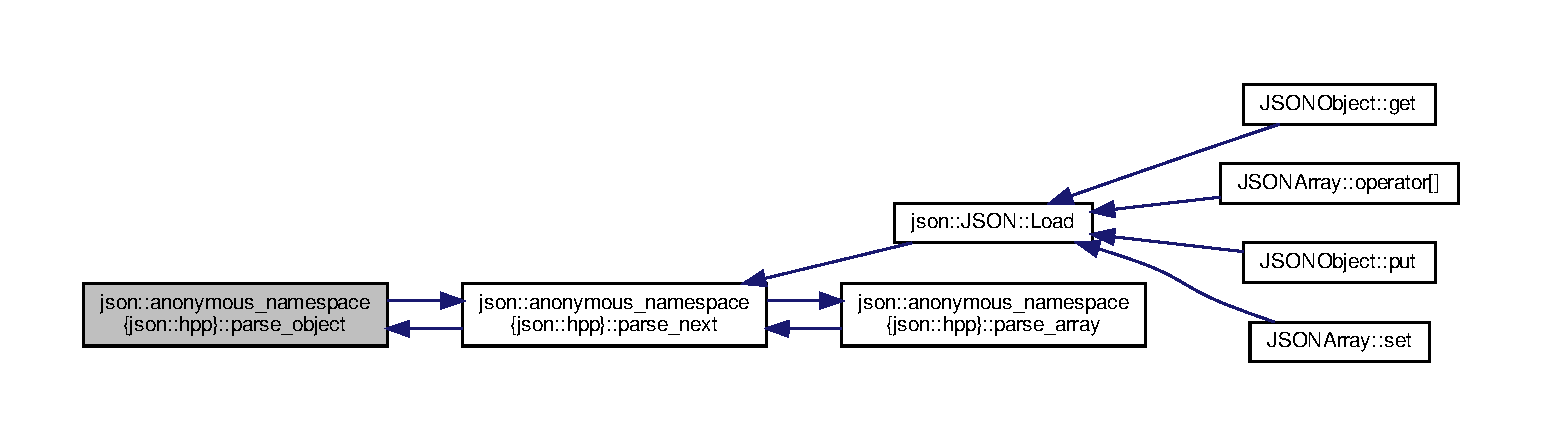
\includegraphics[width=350pt]{namespacejson_1_1anonymous__namespace_02json_8hpp_03_a69b6c8f8bb93130f5c6dab832000f915_icgraph}
\end{center}
\end{figure}
\mbox{\Hypertarget{namespacejson_1_1anonymous__namespace_02json_8hpp_03_a274c7a1f9001093d6b093abb5481122b}\label{namespacejson_1_1anonymous__namespace_02json_8hpp_03_a274c7a1f9001093d6b093abb5481122b}} 
\index{json\+::anonymous\+\_\+namespace\lcurly{}json.\+hpp\rcurly{}@{json\+::anonymous\+\_\+namespace\lcurly{}json.\+hpp\rcurly{}}!parse\+\_\+string@{parse\+\_\+string}}
\index{parse\+\_\+string@{parse\+\_\+string}!json\+::anonymous\+\_\+namespace\lcurly{}json.\+hpp\rcurly{}@{json\+::anonymous\+\_\+namespace\lcurly{}json.\+hpp\rcurly{}}}
\subsubsection{\texorpdfstring{parse\+\_\+string()}{parse\_string()}}
{\footnotesize\ttfamily \mbox{\hyperlink{classjson_1_1_j_s_o_n}{J\+S\+ON}} json\+::anonymous\+\_\+namespace\{json.\+hpp\}\+::parse\+\_\+string (\begin{DoxyParamCaption}\item[{const string \&}]{str,  }\item[{size\+\_\+t \&}]{offset }\end{DoxyParamCaption})}



Definition at line 513 of file json.\+hpp.



References json\+::\+J\+S\+O\+N\+::\+Make(), and json\+::\+J\+S\+O\+N\+::\+String.



Referenced by parse\+\_\+next().


\begin{DoxyCode}
513                                                            \{
514         \mbox{\hyperlink{class_j_s_o_n}{JSON}} String;
515         \textcolor{keywordtype}{string} val;
516         \textcolor{keywordflow}{for}( \textcolor{keywordtype}{char} c = str[++offset]; c != \textcolor{charliteral}{'\(\backslash\)"'} ; c = str[++offset] ) \{
517             \textcolor{keywordflow}{if}( c == \textcolor{charliteral}{'\(\backslash\)\(\backslash\)'} ) \{
518                 \textcolor{keywordflow}{switch}( str[ ++offset ] ) \{
519                 \textcolor{keywordflow}{case} \textcolor{charliteral}{'\(\backslash\)"'}: val += \textcolor{charliteral}{'\(\backslash\)"'}; \textcolor{keywordflow}{break};
520                 \textcolor{keywordflow}{case} \textcolor{charliteral}{'\(\backslash\)\(\backslash\)'}: val += \textcolor{charliteral}{'\(\backslash\)\(\backslash\)'}; \textcolor{keywordflow}{break};
521                 \textcolor{keywordflow}{case} \textcolor{charliteral}{'/'} : val += \textcolor{charliteral}{'/'} ; \textcolor{keywordflow}{break};
522                 \textcolor{keywordflow}{case} \textcolor{charliteral}{'b'} : val += \textcolor{charliteral}{'\(\backslash\)b'}; \textcolor{keywordflow}{break};
523                 \textcolor{keywordflow}{case} \textcolor{charliteral}{'f'} : val += \textcolor{charliteral}{'\(\backslash\)f'}; \textcolor{keywordflow}{break};
524                 \textcolor{keywordflow}{case} \textcolor{charliteral}{'n'} : val += \textcolor{charliteral}{'\(\backslash\)n'}; \textcolor{keywordflow}{break};
525                 \textcolor{keywordflow}{case} \textcolor{charliteral}{'r'} : val += \textcolor{charliteral}{'\(\backslash\)r'}; \textcolor{keywordflow}{break};
526                 \textcolor{keywordflow}{case} \textcolor{charliteral}{'t'} : val += \textcolor{charliteral}{'\(\backslash\)t'}; \textcolor{keywordflow}{break};
527                 \textcolor{keywordflow}{case} \textcolor{charliteral}{'u'} : \{
528                     val += \textcolor{stringliteral}{"\(\backslash\)\(\backslash\)u"} ;
529                     \textcolor{keywordflow}{for}( \textcolor{keywordtype}{unsigned} i = 1; i <= 4; ++i ) \{
530                         c = str[offset+i];
531                         \textcolor{keywordflow}{if}( (c >= \textcolor{charliteral}{'0'} && c <= \textcolor{charliteral}{'9'}) || (c >= \textcolor{charliteral}{'a'} && c <= \textcolor{charliteral}{'f'}) || (c >= \textcolor{charliteral}{'A'} && c <= \textcolor{charliteral}{'F'}) )
532                             val += c;
533                         \textcolor{keywordflow}{else} \{
534                             std::cerr << \textcolor{stringliteral}{"ERROR: String: Expected hex character in unicode escape, found '"}
       << c << \textcolor{stringliteral}{"'\(\backslash\)n"};
535                             \textcolor{keywordflow}{return} std::move( JSON::Make( JSON::Class::String ) );
536                         \}
537                     \}
538                     offset += 4;
539                 \} \textcolor{keywordflow}{break};
540                 default  : val += \textcolor{charliteral}{'\(\backslash\)\(\backslash\)'}; \textcolor{keywordflow}{break};
541                 \}
542             \}
543             \textcolor{keywordflow}{else}
544                 val += c;
545         \}
546         ++offset;
547         String = val;
548         \textcolor{keywordflow}{return} std::move( String );
549     \}
\end{DoxyCode}
Here is the call graph for this function\+:
\nopagebreak
\begin{figure}[H]
\begin{center}
\leavevmode
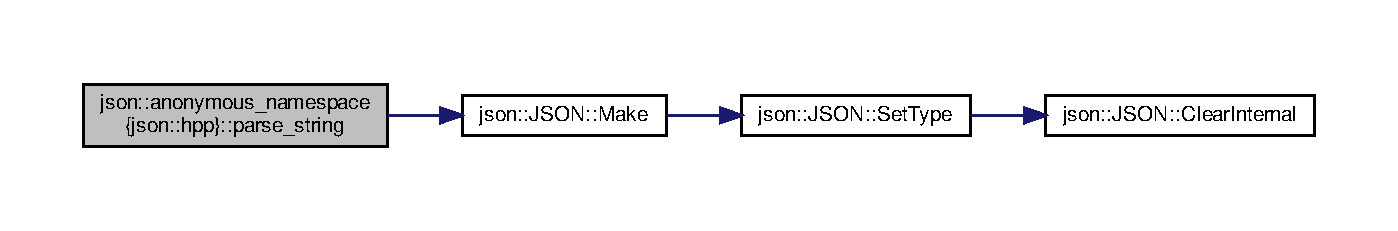
\includegraphics[width=350pt]{namespacejson_1_1anonymous__namespace_02json_8hpp_03_a274c7a1f9001093d6b093abb5481122b_cgraph}
\end{center}
\end{figure}
Here is the caller graph for this function\+:
\nopagebreak
\begin{figure}[H]
\begin{center}
\leavevmode
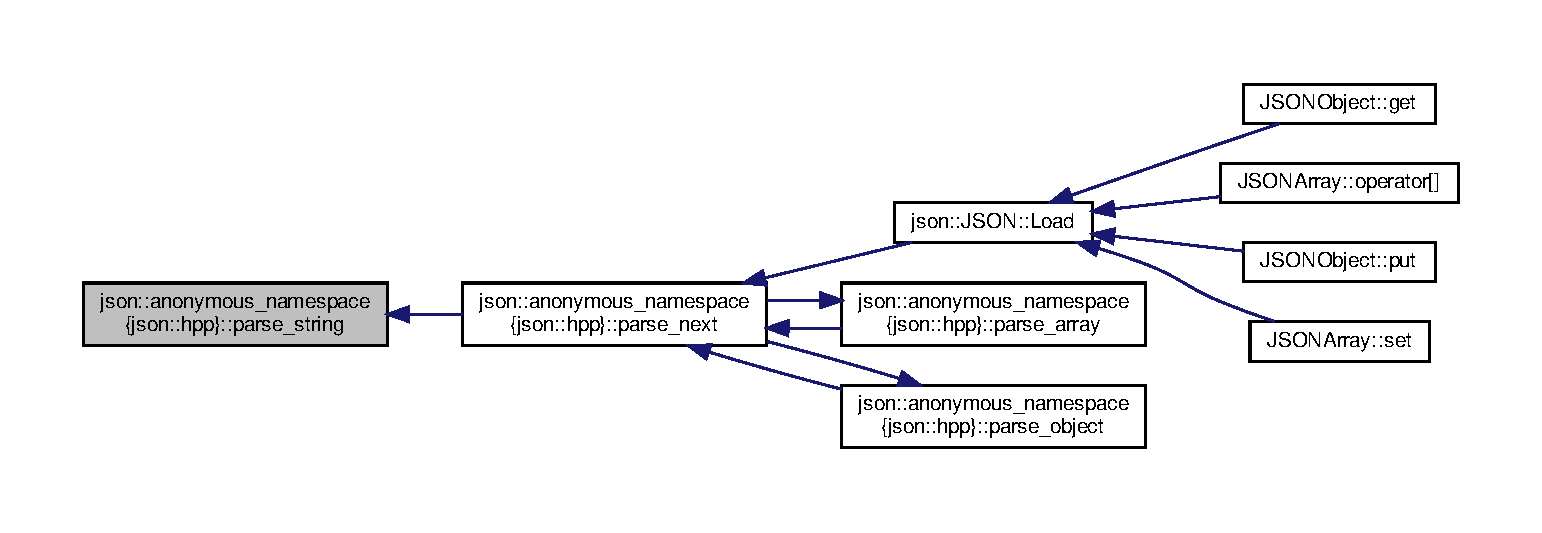
\includegraphics[width=350pt]{namespacejson_1_1anonymous__namespace_02json_8hpp_03_a274c7a1f9001093d6b093abb5481122b_icgraph}
\end{center}
\end{figure}

\chapter{Data Structure Documentation}
\hypertarget{unionjson_1_1_j_s_o_n_1_1_backing_data}{}\section{json\+:\+:J\+S\+ON\+:\+:Backing\+Data Union Reference}
\label{unionjson_1_1_j_s_o_n_1_1_backing_data}\index{json\+::\+J\+S\+O\+N\+::\+Backing\+Data@{json\+::\+J\+S\+O\+N\+::\+Backing\+Data}}


Collaboration diagram for json\+:\+:J\+S\+ON\+:\+:Backing\+Data\+:
\nopagebreak
\begin{figure}[H]
\begin{center}
\leavevmode
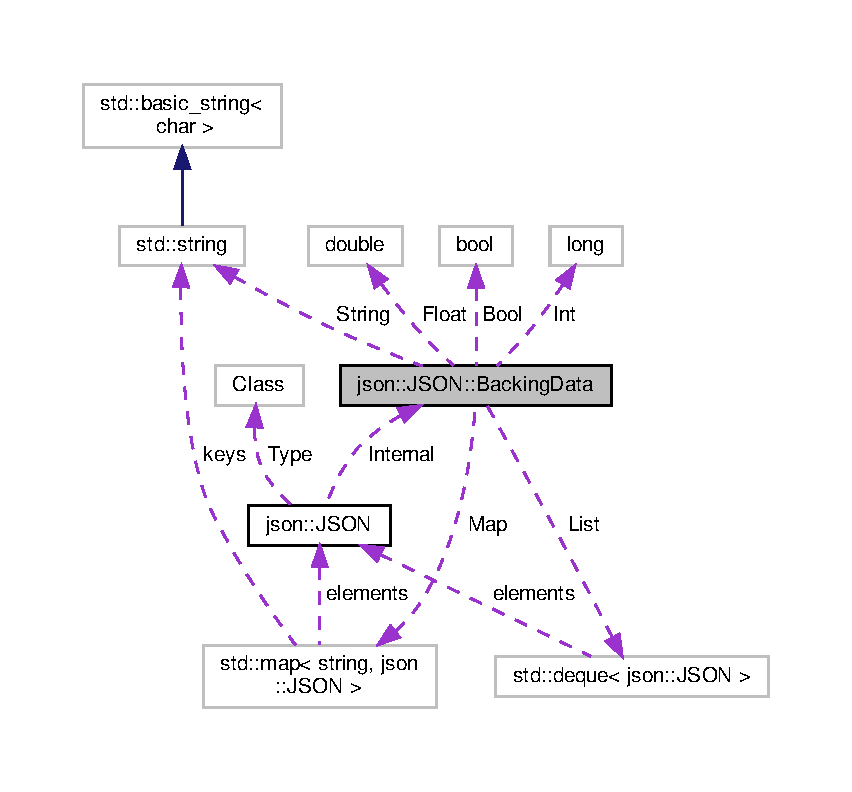
\includegraphics[width=350pt]{unionjson_1_1_j_s_o_n_1_1_backing_data__coll__graph}
\end{center}
\end{figure}
\subsection*{Public Member Functions}
\begin{DoxyCompactItemize}
\item 
\mbox{\hyperlink{unionjson_1_1_j_s_o_n_1_1_backing_data_a7d9921b5b250d942ceb1b2e11a8b9b8b}{Backing\+Data}} (double d)
\item 
\mbox{\hyperlink{unionjson_1_1_j_s_o_n_1_1_backing_data_a25277bc3224f9a7ed291fe209b9294d2}{Backing\+Data}} (long l)
\item 
\mbox{\hyperlink{unionjson_1_1_j_s_o_n_1_1_backing_data_abe54395f8ce5d9918ff0704a4e1bae98}{Backing\+Data}} (bool b)
\item 
\mbox{\hyperlink{unionjson_1_1_j_s_o_n_1_1_backing_data_a05c304ee380de872456ce7679c48b2ce}{Backing\+Data}} (string s)
\item 
\mbox{\hyperlink{unionjson_1_1_j_s_o_n_1_1_backing_data_aeeb02720b7de2606b868f6a2d11c83ea}{Backing\+Data}} ()
\end{DoxyCompactItemize}
\subsection*{Data Fields}
\begin{DoxyCompactItemize}
\item 
deque$<$ \mbox{\hyperlink{classjson_1_1_j_s_o_n}{J\+S\+ON}} $>$ $\ast$ \mbox{\hyperlink{unionjson_1_1_j_s_o_n_1_1_backing_data_ab85f5e7ad21f9f7a5407ab73128a3ebc}{List}}
\item 
map$<$ string, \mbox{\hyperlink{classjson_1_1_j_s_o_n}{J\+S\+ON}} $>$ $\ast$ \mbox{\hyperlink{unionjson_1_1_j_s_o_n_1_1_backing_data_ab2e19b00745b37d2add157ff3a35c431}{Map}}
\item 
string $\ast$ \mbox{\hyperlink{unionjson_1_1_j_s_o_n_1_1_backing_data_a883c18d113d2e55767a9530f06a9c772}{String}}
\item 
double \mbox{\hyperlink{unionjson_1_1_j_s_o_n_1_1_backing_data_aac4950afa6b9205bb367a33de47faa5c}{Float}}
\item 
long \mbox{\hyperlink{unionjson_1_1_j_s_o_n_1_1_backing_data_a0d80815a70ff5bb9345f75de79ec81c3}{Int}}
\item 
bool \mbox{\hyperlink{unionjson_1_1_j_s_o_n_1_1_backing_data_a0659fafaedb7de535ae3e79e4ff4688c}{Bool}}
\end{DoxyCompactItemize}


\subsection{Detailed Description}


Definition at line 47 of file json.\+hpp.



\subsection{Constructor \& Destructor Documentation}
\mbox{\Hypertarget{unionjson_1_1_j_s_o_n_1_1_backing_data_a7d9921b5b250d942ceb1b2e11a8b9b8b}\label{unionjson_1_1_j_s_o_n_1_1_backing_data_a7d9921b5b250d942ceb1b2e11a8b9b8b}} 
\index{json\+::\+J\+S\+O\+N\+::\+Backing\+Data@{json\+::\+J\+S\+O\+N\+::\+Backing\+Data}!Backing\+Data@{Backing\+Data}}
\index{Backing\+Data@{Backing\+Data}!json\+::\+J\+S\+O\+N\+::\+Backing\+Data@{json\+::\+J\+S\+O\+N\+::\+Backing\+Data}}
\subsubsection{\texorpdfstring{Backing\+Data()}{BackingData()}\hspace{0.1cm}{\footnotesize\ttfamily [1/5]}}
{\footnotesize\ttfamily json\+::\+J\+S\+O\+N\+::\+Backing\+Data\+::\+Backing\+Data (\begin{DoxyParamCaption}\item[{double}]{d }\end{DoxyParamCaption})\hspace{0.3cm}{\ttfamily [inline]}}



Definition at line 48 of file json.\+hpp.


\begin{DoxyCode}
48 : \mbox{\hyperlink{unionjson_1_1_j_s_o_n_1_1_backing_data_aac4950afa6b9205bb367a33de47faa5c}{Float}}( d )\{\}
\end{DoxyCode}
\mbox{\Hypertarget{unionjson_1_1_j_s_o_n_1_1_backing_data_a25277bc3224f9a7ed291fe209b9294d2}\label{unionjson_1_1_j_s_o_n_1_1_backing_data_a25277bc3224f9a7ed291fe209b9294d2}} 
\index{json\+::\+J\+S\+O\+N\+::\+Backing\+Data@{json\+::\+J\+S\+O\+N\+::\+Backing\+Data}!Backing\+Data@{Backing\+Data}}
\index{Backing\+Data@{Backing\+Data}!json\+::\+J\+S\+O\+N\+::\+Backing\+Data@{json\+::\+J\+S\+O\+N\+::\+Backing\+Data}}
\subsubsection{\texorpdfstring{Backing\+Data()}{BackingData()}\hspace{0.1cm}{\footnotesize\ttfamily [2/5]}}
{\footnotesize\ttfamily json\+::\+J\+S\+O\+N\+::\+Backing\+Data\+::\+Backing\+Data (\begin{DoxyParamCaption}\item[{long}]{l }\end{DoxyParamCaption})\hspace{0.3cm}{\ttfamily [inline]}}



Definition at line 49 of file json.\+hpp.


\begin{DoxyCode}
49 : \mbox{\hyperlink{unionjson_1_1_j_s_o_n_1_1_backing_data_a0d80815a70ff5bb9345f75de79ec81c3}{Int}}( l )\{\}
\end{DoxyCode}
\mbox{\Hypertarget{unionjson_1_1_j_s_o_n_1_1_backing_data_abe54395f8ce5d9918ff0704a4e1bae98}\label{unionjson_1_1_j_s_o_n_1_1_backing_data_abe54395f8ce5d9918ff0704a4e1bae98}} 
\index{json\+::\+J\+S\+O\+N\+::\+Backing\+Data@{json\+::\+J\+S\+O\+N\+::\+Backing\+Data}!Backing\+Data@{Backing\+Data}}
\index{Backing\+Data@{Backing\+Data}!json\+::\+J\+S\+O\+N\+::\+Backing\+Data@{json\+::\+J\+S\+O\+N\+::\+Backing\+Data}}
\subsubsection{\texorpdfstring{Backing\+Data()}{BackingData()}\hspace{0.1cm}{\footnotesize\ttfamily [3/5]}}
{\footnotesize\ttfamily json\+::\+J\+S\+O\+N\+::\+Backing\+Data\+::\+Backing\+Data (\begin{DoxyParamCaption}\item[{bool}]{b }\end{DoxyParamCaption})\hspace{0.3cm}{\ttfamily [inline]}}



Definition at line 50 of file json.\+hpp.


\begin{DoxyCode}
50 : \mbox{\hyperlink{unionjson_1_1_j_s_o_n_1_1_backing_data_a0659fafaedb7de535ae3e79e4ff4688c}{Bool}}( b )\{\}
\end{DoxyCode}
\mbox{\Hypertarget{unionjson_1_1_j_s_o_n_1_1_backing_data_a05c304ee380de872456ce7679c48b2ce}\label{unionjson_1_1_j_s_o_n_1_1_backing_data_a05c304ee380de872456ce7679c48b2ce}} 
\index{json\+::\+J\+S\+O\+N\+::\+Backing\+Data@{json\+::\+J\+S\+O\+N\+::\+Backing\+Data}!Backing\+Data@{Backing\+Data}}
\index{Backing\+Data@{Backing\+Data}!json\+::\+J\+S\+O\+N\+::\+Backing\+Data@{json\+::\+J\+S\+O\+N\+::\+Backing\+Data}}
\subsubsection{\texorpdfstring{Backing\+Data()}{BackingData()}\hspace{0.1cm}{\footnotesize\ttfamily [4/5]}}
{\footnotesize\ttfamily json\+::\+J\+S\+O\+N\+::\+Backing\+Data\+::\+Backing\+Data (\begin{DoxyParamCaption}\item[{string}]{s }\end{DoxyParamCaption})\hspace{0.3cm}{\ttfamily [inline]}}



Definition at line 51 of file json.\+hpp.


\begin{DoxyCode}
51 : \mbox{\hyperlink{unionjson_1_1_j_s_o_n_1_1_backing_data_a883c18d113d2e55767a9530f06a9c772}{String}}( \textcolor{keyword}{new} \textcolor{keywordtype}{string}( s ) )\{\}
\end{DoxyCode}
\mbox{\Hypertarget{unionjson_1_1_j_s_o_n_1_1_backing_data_aeeb02720b7de2606b868f6a2d11c83ea}\label{unionjson_1_1_j_s_o_n_1_1_backing_data_aeeb02720b7de2606b868f6a2d11c83ea}} 
\index{json\+::\+J\+S\+O\+N\+::\+Backing\+Data@{json\+::\+J\+S\+O\+N\+::\+Backing\+Data}!Backing\+Data@{Backing\+Data}}
\index{Backing\+Data@{Backing\+Data}!json\+::\+J\+S\+O\+N\+::\+Backing\+Data@{json\+::\+J\+S\+O\+N\+::\+Backing\+Data}}
\subsubsection{\texorpdfstring{Backing\+Data()}{BackingData()}\hspace{0.1cm}{\footnotesize\ttfamily [5/5]}}
{\footnotesize\ttfamily json\+::\+J\+S\+O\+N\+::\+Backing\+Data\+::\+Backing\+Data (\begin{DoxyParamCaption}{ }\end{DoxyParamCaption})\hspace{0.3cm}{\ttfamily [inline]}}



Definition at line 52 of file json.\+hpp.


\begin{DoxyCode}
52 : \mbox{\hyperlink{unionjson_1_1_j_s_o_n_1_1_backing_data_a0d80815a70ff5bb9345f75de79ec81c3}{Int}}( 0 )\{\}
\end{DoxyCode}


\subsection{Field Documentation}
\mbox{\Hypertarget{unionjson_1_1_j_s_o_n_1_1_backing_data_a0659fafaedb7de535ae3e79e4ff4688c}\label{unionjson_1_1_j_s_o_n_1_1_backing_data_a0659fafaedb7de535ae3e79e4ff4688c}} 
\index{json\+::\+J\+S\+O\+N\+::\+Backing\+Data@{json\+::\+J\+S\+O\+N\+::\+Backing\+Data}!Bool@{Bool}}
\index{Bool@{Bool}!json\+::\+J\+S\+O\+N\+::\+Backing\+Data@{json\+::\+J\+S\+O\+N\+::\+Backing\+Data}}
\subsubsection{\texorpdfstring{Bool}{Bool}}
{\footnotesize\ttfamily bool json\+::\+J\+S\+O\+N\+::\+Backing\+Data\+::\+Bool}



Definition at line 59 of file json.\+hpp.



Referenced by json\+::\+J\+S\+O\+N\+::dump(), json\+::\+J\+S\+O\+N\+::operator=(), json\+::\+J\+S\+O\+N\+::\+Set\+Type(), and json\+::\+J\+S\+O\+N\+::\+To\+Bool().

\mbox{\Hypertarget{unionjson_1_1_j_s_o_n_1_1_backing_data_aac4950afa6b9205bb367a33de47faa5c}\label{unionjson_1_1_j_s_o_n_1_1_backing_data_aac4950afa6b9205bb367a33de47faa5c}} 
\index{json\+::\+J\+S\+O\+N\+::\+Backing\+Data@{json\+::\+J\+S\+O\+N\+::\+Backing\+Data}!Float@{Float}}
\index{Float@{Float}!json\+::\+J\+S\+O\+N\+::\+Backing\+Data@{json\+::\+J\+S\+O\+N\+::\+Backing\+Data}}
\subsubsection{\texorpdfstring{Float}{Float}}
{\footnotesize\ttfamily double json\+::\+J\+S\+O\+N\+::\+Backing\+Data\+::\+Float}



Definition at line 57 of file json.\+hpp.



Referenced by json\+::\+J\+S\+O\+N\+::dump(), json\+::\+J\+S\+O\+N\+::operator=(), json\+::\+J\+S\+O\+N\+::\+Set\+Type(), and json\+::\+J\+S\+O\+N\+::\+To\+Float().

\mbox{\Hypertarget{unionjson_1_1_j_s_o_n_1_1_backing_data_a0d80815a70ff5bb9345f75de79ec81c3}\label{unionjson_1_1_j_s_o_n_1_1_backing_data_a0d80815a70ff5bb9345f75de79ec81c3}} 
\index{json\+::\+J\+S\+O\+N\+::\+Backing\+Data@{json\+::\+J\+S\+O\+N\+::\+Backing\+Data}!Int@{Int}}
\index{Int@{Int}!json\+::\+J\+S\+O\+N\+::\+Backing\+Data@{json\+::\+J\+S\+O\+N\+::\+Backing\+Data}}
\subsubsection{\texorpdfstring{Int}{Int}}
{\footnotesize\ttfamily long json\+::\+J\+S\+O\+N\+::\+Backing\+Data\+::\+Int}



Definition at line 58 of file json.\+hpp.



Referenced by json\+::\+J\+S\+O\+N\+::dump(), json\+::\+J\+S\+O\+N\+::operator=(), json\+::\+J\+S\+O\+N\+::\+Set\+Type(), and json\+::\+J\+S\+O\+N\+::\+To\+Int().

\mbox{\Hypertarget{unionjson_1_1_j_s_o_n_1_1_backing_data_ab85f5e7ad21f9f7a5407ab73128a3ebc}\label{unionjson_1_1_j_s_o_n_1_1_backing_data_ab85f5e7ad21f9f7a5407ab73128a3ebc}} 
\index{json\+::\+J\+S\+O\+N\+::\+Backing\+Data@{json\+::\+J\+S\+O\+N\+::\+Backing\+Data}!List@{List}}
\index{List@{List}!json\+::\+J\+S\+O\+N\+::\+Backing\+Data@{json\+::\+J\+S\+O\+N\+::\+Backing\+Data}}
\subsubsection{\texorpdfstring{List}{List}}
{\footnotesize\ttfamily deque$<$\mbox{\hyperlink{classjson_1_1_j_s_o_n}{J\+S\+ON}}$>$$\ast$ json\+::\+J\+S\+O\+N\+::\+Backing\+Data\+::\+List}



Definition at line 54 of file json.\+hpp.



Referenced by json\+::\+J\+S\+O\+N\+::append(), json\+::\+J\+S\+O\+N\+::\+Array\+Range(), json\+::\+J\+S\+O\+N\+::at(), json\+::\+J\+S\+O\+N\+::\+Clear\+Internal(), json\+::\+J\+S\+O\+N\+::dump(), json\+::\+J\+S\+O\+N\+::\+J\+S\+O\+N(), json\+::\+J\+S\+O\+N\+::length(), json\+::\+J\+S\+O\+N\+::operator=(), json\+::\+J\+S\+O\+N\+::operator\mbox{[}$\,$\mbox{]}(), json\+::\+J\+S\+O\+N\+::\+Set\+Type(), json\+::\+J\+S\+O\+N\+::size(), and json\+::\+J\+S\+O\+N\+::$\sim$\+J\+S\+O\+N().

\mbox{\Hypertarget{unionjson_1_1_j_s_o_n_1_1_backing_data_ab2e19b00745b37d2add157ff3a35c431}\label{unionjson_1_1_j_s_o_n_1_1_backing_data_ab2e19b00745b37d2add157ff3a35c431}} 
\index{json\+::\+J\+S\+O\+N\+::\+Backing\+Data@{json\+::\+J\+S\+O\+N\+::\+Backing\+Data}!Map@{Map}}
\index{Map@{Map}!json\+::\+J\+S\+O\+N\+::\+Backing\+Data@{json\+::\+J\+S\+O\+N\+::\+Backing\+Data}}
\subsubsection{\texorpdfstring{Map}{Map}}
{\footnotesize\ttfamily map$<$string,\mbox{\hyperlink{classjson_1_1_j_s_o_n}{J\+S\+ON}}$>$$\ast$ json\+::\+J\+S\+O\+N\+::\+Backing\+Data\+::\+Map}



Definition at line 55 of file json.\+hpp.



Referenced by json\+::\+J\+S\+O\+N\+::at(), json\+::\+J\+S\+O\+N\+::\+Clear\+Internal(), json\+::\+J\+S\+O\+N\+::dump(), json\+::\+J\+S\+O\+N\+::has\+Key(), json\+::\+J\+S\+O\+N\+::\+J\+S\+O\+N(), json\+::\+J\+S\+O\+N\+::\+Object\+Range(), json\+::\+J\+S\+O\+N\+::operator=(), json\+::\+J\+S\+O\+N\+::operator\mbox{[}$\,$\mbox{]}(), json\+::\+J\+S\+O\+N\+::\+Set\+Type(), json\+::\+J\+S\+O\+N\+::size(), and json\+::\+J\+S\+O\+N\+::$\sim$\+J\+S\+O\+N().

\mbox{\Hypertarget{unionjson_1_1_j_s_o_n_1_1_backing_data_a883c18d113d2e55767a9530f06a9c772}\label{unionjson_1_1_j_s_o_n_1_1_backing_data_a883c18d113d2e55767a9530f06a9c772}} 
\index{json\+::\+J\+S\+O\+N\+::\+Backing\+Data@{json\+::\+J\+S\+O\+N\+::\+Backing\+Data}!String@{String}}
\index{String@{String}!json\+::\+J\+S\+O\+N\+::\+Backing\+Data@{json\+::\+J\+S\+O\+N\+::\+Backing\+Data}}
\subsubsection{\texorpdfstring{String}{String}}
{\footnotesize\ttfamily string$\ast$ json\+::\+J\+S\+O\+N\+::\+Backing\+Data\+::\+String}



Definition at line 56 of file json.\+hpp.



Referenced by json\+::\+J\+S\+O\+N\+::\+Clear\+Internal(), json\+::\+J\+S\+O\+N\+::dump(), json\+::\+J\+S\+O\+N\+::\+J\+S\+O\+N(), json\+::\+J\+S\+O\+N\+::operator=(), json\+::\+J\+S\+O\+N\+::\+Set\+Type(), json\+::\+J\+S\+O\+N\+::\+To\+String(), and json\+::\+J\+S\+O\+N\+::$\sim$\+J\+S\+O\+N().



The documentation for this union was generated from the following file\+:\begin{DoxyCompactItemize}
\item 
lib/simplejson/\mbox{\hyperlink{lib_2simplejson_2json_8hpp}{json.\+hpp}}\end{DoxyCompactItemize}

\hypertarget{class_complex_instruktion}{}\section{Complex\+Instruktion Class Reference}
\label{class_complex_instruktion}\index{Complex\+Instruktion@{Complex\+Instruktion}}


{\ttfamily \#include $<$instruction.\+hpp$>$}



Inheritance diagram for Complex\+Instruktion\+:
\nopagebreak
\begin{figure}[H]
\begin{center}
\leavevmode
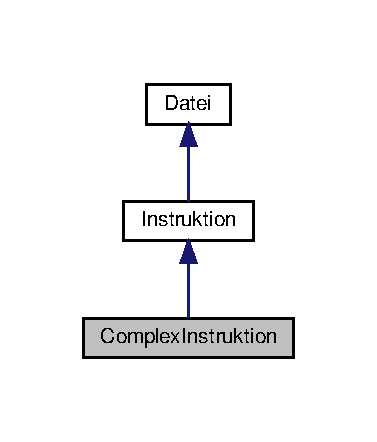
\includegraphics[width=181pt]{class_complex_instruktion__inherit__graph}
\end{center}
\end{figure}


Collaboration diagram for Complex\+Instruktion\+:
\nopagebreak
\begin{figure}[H]
\begin{center}
\leavevmode
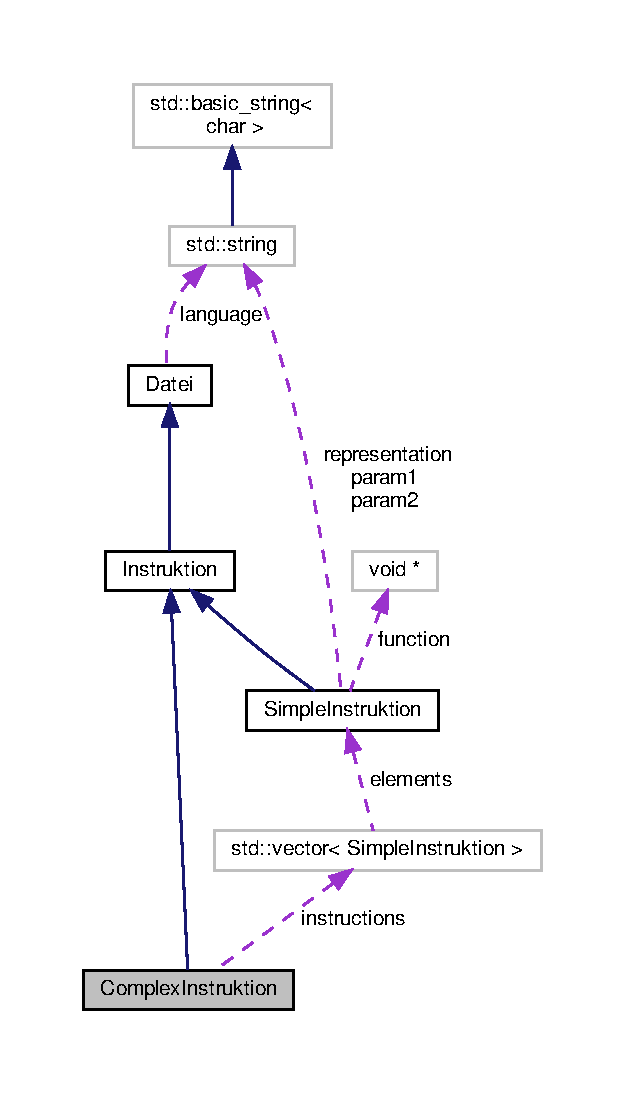
\includegraphics[width=300pt]{class_complex_instruktion__coll__graph}
\end{center}
\end{figure}
\subsection*{Public Member Functions}
\begin{DoxyCompactItemize}
\item 
\mbox{\hyperlink{class_complex_instruktion_a954dad29a6453083400008671c0c05eb}{Complex\+Instruktion}} (std\+::string)
\item 
\mbox{\hyperlink{class_complex_instruktion_a781aafaec2554b759f887f2667272f06}{Complex\+Instruktion}} (std\+::string, \mbox{\hyperlink{class_simple_instruktion}{Simple\+Instruktion}} \&)
\item 
std\+::string \mbox{\hyperlink{class_complex_instruktion_a476d0f6ed0296cd4751543c4be6ca422}{print}} ()
\item 
void \mbox{\hyperlink{class_complex_instruktion_ab9e037eda3cf53252902f15541a01a21}{run}} (\mbox{\hyperlink{class_virtual_machine}{Virtual\+Machine}} \&)
\item 
void \mbox{\hyperlink{class_complex_instruktion_ae92fcdd92e0328d4eed826dea81b8c9c}{add}} (\mbox{\hyperlink{class_simple_instruktion}{Simple\+Instruktion}} \&)
\end{DoxyCompactItemize}
\subsection*{Private Attributes}
\begin{DoxyCompactItemize}
\item 
std\+::vector$<$ \mbox{\hyperlink{class_simple_instruktion}{Simple\+Instruktion}} $>$ \mbox{\hyperlink{class_complex_instruktion_af8a7ed862ee24675b75750a470dcf22a}{instructions}}
\end{DoxyCompactItemize}
\subsection*{Additional Inherited Members}


\subsection{Detailed Description}
Klasse für mehrerern Instruktionen. Funktioniert wie eine klügere Array (aber komplexer, auch). 

Definition at line 42 of file instruction.\+hpp.



\subsection{Constructor \& Destructor Documentation}
\mbox{\Hypertarget{class_complex_instruktion_a954dad29a6453083400008671c0c05eb}\label{class_complex_instruktion_a954dad29a6453083400008671c0c05eb}} 
\index{Complex\+Instruktion@{Complex\+Instruktion}!Complex\+Instruktion@{Complex\+Instruktion}}
\index{Complex\+Instruktion@{Complex\+Instruktion}!Complex\+Instruktion@{Complex\+Instruktion}}
\subsubsection{\texorpdfstring{Complex\+Instruktion()}{ComplexInstruktion()}\hspace{0.1cm}{\footnotesize\ttfamily [1/2]}}
{\footnotesize\ttfamily Complex\+Instruktion\+::\+Complex\+Instruktion (\begin{DoxyParamCaption}\item[{std\+::string}]{lang }\end{DoxyParamCaption})}

Initialisiert \mbox{\hyperlink{class_complex_instruktion}{Complex\+Instruktion}} nur mit der \mbox{\hyperlink{class_sprache}{Sprache}}. 

Definition at line 35 of file instruction.\+cpp.


\begin{DoxyCode}
35                                                      : \mbox{\hyperlink{class_instruktion_a26d54febd2022c7402a22a8b55ba097a}{Instruktion}}(lang)
36 \{
37 \}
\end{DoxyCode}
\mbox{\Hypertarget{class_complex_instruktion_a781aafaec2554b759f887f2667272f06}\label{class_complex_instruktion_a781aafaec2554b759f887f2667272f06}} 
\index{Complex\+Instruktion@{Complex\+Instruktion}!Complex\+Instruktion@{Complex\+Instruktion}}
\index{Complex\+Instruktion@{Complex\+Instruktion}!Complex\+Instruktion@{Complex\+Instruktion}}
\subsubsection{\texorpdfstring{Complex\+Instruktion()}{ComplexInstruktion()}\hspace{0.1cm}{\footnotesize\ttfamily [2/2]}}
{\footnotesize\ttfamily Complex\+Instruktion\+::\+Complex\+Instruktion (\begin{DoxyParamCaption}\item[{std\+::string}]{lang,  }\item[{\mbox{\hyperlink{class_simple_instruktion}{Simple\+Instruktion}} \&}]{begin }\end{DoxyParamCaption})}

Initialisiert \mbox{\hyperlink{class_complex_instruktion}{Complex\+Instruktion}} sowohl mit der \mbox{\hyperlink{class_sprache}{Sprache}} als auch mit einem \mbox{\hyperlink{class_simple_instruktion}{Simple\+Instruktion}}. 

Definition at line 43 of file instruction.\+cpp.



References instructions.


\begin{DoxyCode}
43                                                                                : 
      \mbox{\hyperlink{class_instruktion_a26d54febd2022c7402a22a8b55ba097a}{Instruktion}}(lang)
44 \{
45     \mbox{\hyperlink{class_complex_instruktion_af8a7ed862ee24675b75750a470dcf22a}{instructions}}.push\_back(begin);
46 \}
\end{DoxyCode}


\subsection{Member Function Documentation}
\mbox{\Hypertarget{class_complex_instruktion_ae92fcdd92e0328d4eed826dea81b8c9c}\label{class_complex_instruktion_ae92fcdd92e0328d4eed826dea81b8c9c}} 
\index{Complex\+Instruktion@{Complex\+Instruktion}!add@{add}}
\index{add@{add}!Complex\+Instruktion@{Complex\+Instruktion}}
\subsubsection{\texorpdfstring{add()}{add()}}
{\footnotesize\ttfamily void Complex\+Instruktion\+::add (\begin{DoxyParamCaption}\item[{\mbox{\hyperlink{class_simple_instruktion}{Simple\+Instruktion}} \&}]{si }\end{DoxyParamCaption})}

Eine neue \mbox{\hyperlink{class_simple_instruktion}{Simple\+Instruktion}} einfügen. 

Definition at line 77 of file instruction.\+cpp.



References instructions.



Referenced by Virtual\+Machine\+::add\+Subroutine().


\begin{DoxyCode}
78 \{
79     \mbox{\hyperlink{class_complex_instruktion_af8a7ed862ee24675b75750a470dcf22a}{instructions}}.push\_back(si);
80 \}
\end{DoxyCode}
Here is the caller graph for this function\+:
\nopagebreak
\begin{figure}[H]
\begin{center}
\leavevmode
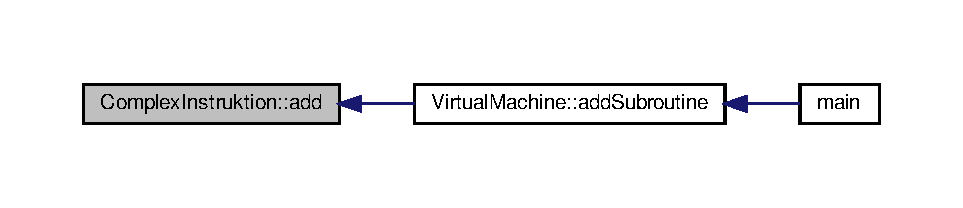
\includegraphics[width=350pt]{class_complex_instruktion_ae92fcdd92e0328d4eed826dea81b8c9c_icgraph}
\end{center}
\end{figure}
\mbox{\Hypertarget{class_complex_instruktion_a476d0f6ed0296cd4751543c4be6ca422}\label{class_complex_instruktion_a476d0f6ed0296cd4751543c4be6ca422}} 
\index{Complex\+Instruktion@{Complex\+Instruktion}!print@{print}}
\index{print@{print}!Complex\+Instruktion@{Complex\+Instruktion}}
\subsubsection{\texorpdfstring{print()}{print()}}
{\footnotesize\ttfamily std\+::string Complex\+Instruktion\+::print (\begin{DoxyParamCaption}{ }\end{DoxyParamCaption})\hspace{0.3cm}{\ttfamily [virtual]}}

Gibt die String-\/\+Representation des ganzen Instruktionenliste zurück. 

Implements \mbox{\hyperlink{class_instruktion_a267ff36e98ec889cceccb2f464c36bc6}{Instruktion}}.



Definition at line 52 of file instruction.\+cpp.



References instructions.


\begin{DoxyCode}
53 \{
54     std::string ret = \textcolor{stringliteral}{""};
55     \textcolor{keywordflow}{for}(\mbox{\hyperlink{class_simple_instruktion}{SimpleInstruktion}} si : \mbox{\hyperlink{class_complex_instruktion_af8a7ed862ee24675b75750a470dcf22a}{instructions}})
56     \{
57         ret+=si.print()+=\textcolor{charliteral}{'\(\backslash\)n'};
58     \}
59     \textcolor{keywordflow}{return} ret;
60 \}
\end{DoxyCode}
\mbox{\Hypertarget{class_complex_instruktion_ab9e037eda3cf53252902f15541a01a21}\label{class_complex_instruktion_ab9e037eda3cf53252902f15541a01a21}} 
\index{Complex\+Instruktion@{Complex\+Instruktion}!run@{run}}
\index{run@{run}!Complex\+Instruktion@{Complex\+Instruktion}}
\subsubsection{\texorpdfstring{run()}{run()}}
{\footnotesize\ttfamily void Complex\+Instruktion\+::run (\begin{DoxyParamCaption}\item[{\mbox{\hyperlink{class_virtual_machine}{Virtual\+Machine}} \&}]{vm }\end{DoxyParamCaption})\hspace{0.3cm}{\ttfamily [virtual]}}

Ausführt jede \mbox{\hyperlink{class_instruktion}{Instruktion}}, denen sie enthielt. 

Implements \mbox{\hyperlink{class_instruktion_ad701f6b5537e5aa8c8c08b81a8946f63}{Instruktion}}.



Definition at line 65 of file instruction.\+cpp.



References instructions.


\begin{DoxyCode}
66 \{
67     \textcolor{keywordflow}{for}(\mbox{\hyperlink{class_simple_instruktion}{SimpleInstruktion}} si : \mbox{\hyperlink{class_complex_instruktion_af8a7ed862ee24675b75750a470dcf22a}{instructions}})
68     \{
69         si.run(vm);
70     \}
71 \}
\end{DoxyCode}


\subsection{Field Documentation}
\mbox{\Hypertarget{class_complex_instruktion_af8a7ed862ee24675b75750a470dcf22a}\label{class_complex_instruktion_af8a7ed862ee24675b75750a470dcf22a}} 
\index{Complex\+Instruktion@{Complex\+Instruktion}!instructions@{instructions}}
\index{instructions@{instructions}!Complex\+Instruktion@{Complex\+Instruktion}}
\subsubsection{\texorpdfstring{instructions}{instructions}}
{\footnotesize\ttfamily std\+::vector$<$\mbox{\hyperlink{class_simple_instruktion}{Simple\+Instruktion}}$>$ Complex\+Instruktion\+::instructions\hspace{0.3cm}{\ttfamily [private]}}



Definition at line 45 of file instruction.\+hpp.



Referenced by add(), Complex\+Instruktion(), print(), and run().



The documentation for this class was generated from the following files\+:\begin{DoxyCompactItemize}
\item 
src/datei/instruction/\mbox{\hyperlink{instruction_8hpp}{instruction.\+hpp}}\item 
src/datei/instruction/\mbox{\hyperlink{instruction_8cpp}{instruction.\+cpp}}\end{DoxyCompactItemize}

\hypertarget{class_datei}{}\section{Datei Class Reference}
\label{class_datei}\index{Datei@{Datei}}


{\ttfamily \#include $<$datei.\+hpp$>$}



Inheritance diagram for Datei\+:
\nopagebreak
\begin{figure}[H]
\begin{center}
\leavevmode
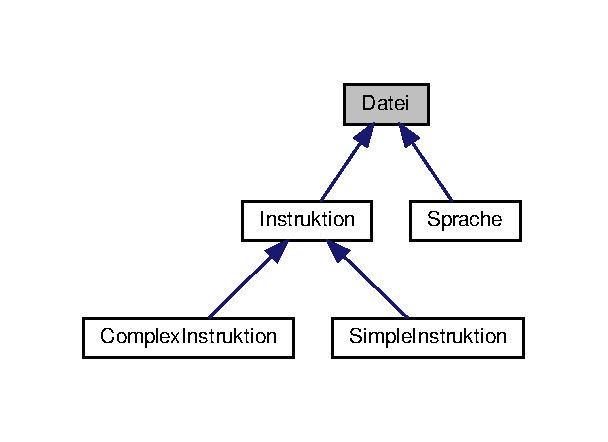
\includegraphics[width=292pt]{class_datei__inherit__graph}
\end{center}
\end{figure}


Collaboration diagram for Datei\+:
\nopagebreak
\begin{figure}[H]
\begin{center}
\leavevmode
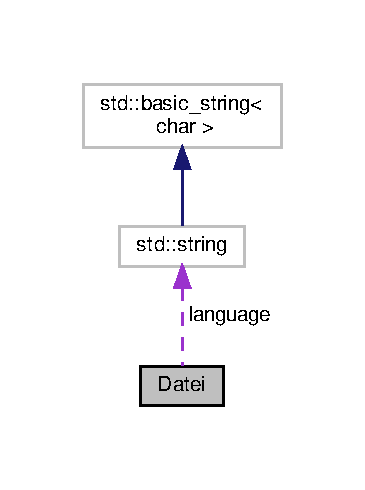
\includegraphics[width=175pt]{class_datei__coll__graph}
\end{center}
\end{figure}
\subsection*{Public Member Functions}
\begin{DoxyCompactItemize}
\item 
\mbox{\hyperlink{class_datei_a9a9e1149154603548fdfc889821cf418}{Datei}} (std\+::string)
\item 
virtual std\+::string \mbox{\hyperlink{class_datei_a5dedc9776ebe637f0842300f648d4b17}{print}} ()=0
\item 
std\+::string \mbox{\hyperlink{class_datei_aeeaf8e269f4d2b53e209ad905b5b75c5}{get\+Lang}} ()
\end{DoxyCompactItemize}
\subsection*{Protected Attributes}
\begin{DoxyCompactItemize}
\item 
std\+::string \mbox{\hyperlink{class_datei_a49b90e65e1e9523b2a61e370727d9510}{language}}
\end{DoxyCompactItemize}
\subsection*{Friends}
\begin{DoxyCompactItemize}
\item 
std\+::ostream \& \mbox{\hyperlink{class_datei_aca7b8a47eeafb9d0860bebec55d21923}{operator$<$$<$}} (std\+::ostream \&, \mbox{\hyperlink{class_datei}{Datei}} \&)
\end{DoxyCompactItemize}


\subsection{Detailed Description}
Klasse für Dateien. 

Definition at line 10 of file datei.\+hpp.



\subsection{Constructor \& Destructor Documentation}
\mbox{\Hypertarget{class_datei_a9a9e1149154603548fdfc889821cf418}\label{class_datei_a9a9e1149154603548fdfc889821cf418}} 
\index{Datei@{Datei}!Datei@{Datei}}
\index{Datei@{Datei}!Datei@{Datei}}
\subsubsection{\texorpdfstring{Datei()}{Datei()}}
{\footnotesize\ttfamily Datei\+::\+Datei (\begin{DoxyParamCaption}\item[{std\+::string}]{lang }\end{DoxyParamCaption})}

Konstruktor für Dateien, stellt die \mbox{\hyperlink{class_sprache}{Sprache}} ein. 

Definition at line 7 of file datei.\+cpp.


\begin{DoxyCode}
7 : \mbox{\hyperlink{class_datei_a49b90e65e1e9523b2a61e370727d9510}{language}}(lang) \{\}
\end{DoxyCode}


\subsection{Member Function Documentation}
\mbox{\Hypertarget{class_datei_aeeaf8e269f4d2b53e209ad905b5b75c5}\label{class_datei_aeeaf8e269f4d2b53e209ad905b5b75c5}} 
\index{Datei@{Datei}!get\+Lang@{get\+Lang}}
\index{get\+Lang@{get\+Lang}!Datei@{Datei}}
\subsubsection{\texorpdfstring{get\+Lang()}{getLang()}}
{\footnotesize\ttfamily std\+::string Datei\+::get\+Lang (\begin{DoxyParamCaption}{ }\end{DoxyParamCaption})}

Getterfunktion für die \mbox{\hyperlink{class_sprache}{Sprache}}. 

Definition at line 22 of file datei.\+cpp.



References language.



Referenced by Virtual\+Machine\+::add\+Subroutine(), Virtual\+Machine\+::run\+Instruction(), and Virtual\+Machine\+::\+Virtual\+Machine().


\begin{DoxyCode}
22 \{ \textcolor{keywordflow}{return} \mbox{\hyperlink{class_datei_a49b90e65e1e9523b2a61e370727d9510}{language}};\}
\end{DoxyCode}
Here is the caller graph for this function\+:
\nopagebreak
\begin{figure}[H]
\begin{center}
\leavevmode
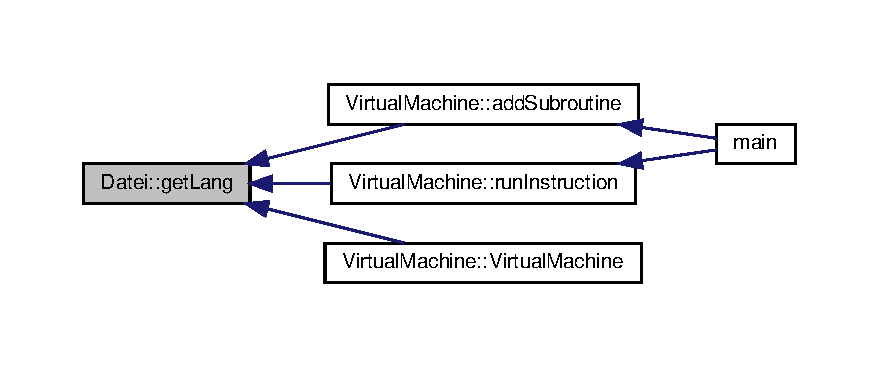
\includegraphics[width=350pt]{class_datei_aeeaf8e269f4d2b53e209ad905b5b75c5_icgraph}
\end{center}
\end{figure}
\mbox{\Hypertarget{class_datei_a5dedc9776ebe637f0842300f648d4b17}\label{class_datei_a5dedc9776ebe637f0842300f648d4b17}} 
\index{Datei@{Datei}!print@{print}}
\index{print@{print}!Datei@{Datei}}
\subsubsection{\texorpdfstring{print()}{print()}}
{\footnotesize\ttfamily virtual std\+::string Datei\+::print (\begin{DoxyParamCaption}{ }\end{DoxyParamCaption})\hspace{0.3cm}{\ttfamily [pure virtual]}}



Implemented in \mbox{\hyperlink{class_complex_instruktion_a476d0f6ed0296cd4751543c4be6ca422}{Complex\+Instruktion}}, \mbox{\hyperlink{class_simple_instruktion_a0533865319bd39a0ecd1db463d488cb8}{Simple\+Instruktion}}, \mbox{\hyperlink{class_sprache_a1e1e39e91e6d33e068fed01333fa99cc}{Sprache}}, and \mbox{\hyperlink{class_instruktion_a267ff36e98ec889cceccb2f464c36bc6}{Instruktion}}.



Referenced by operator$<$$<$().

Here is the caller graph for this function\+:
\nopagebreak
\begin{figure}[H]
\begin{center}
\leavevmode
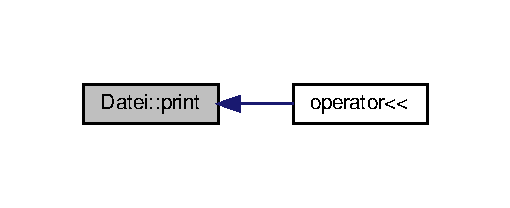
\includegraphics[width=245pt]{class_datei_a5dedc9776ebe637f0842300f648d4b17_icgraph}
\end{center}
\end{figure}


\subsection{Friends And Related Function Documentation}
\mbox{\Hypertarget{class_datei_aca7b8a47eeafb9d0860bebec55d21923}\label{class_datei_aca7b8a47eeafb9d0860bebec55d21923}} 
\index{Datei@{Datei}!operator$<$$<$@{operator$<$$<$}}
\index{operator$<$$<$@{operator$<$$<$}!Datei@{Datei}}
\subsubsection{\texorpdfstring{operator$<$$<$}{operator<<}}
{\footnotesize\ttfamily std\+::ostream\& operator$<$$<$ (\begin{DoxyParamCaption}\item[{std\+::ostream \&}]{os,  }\item[{\mbox{\hyperlink{class_datei}{Datei}} \&}]{d }\end{DoxyParamCaption})\hspace{0.3cm}{\ttfamily [friend]}}

Auschreiben. 

Definition at line 13 of file datei.\+cpp.


\begin{DoxyCode}
14 \{
15     os<<d.\mbox{\hyperlink{class_datei_a5dedc9776ebe637f0842300f648d4b17}{print}}();
16     \textcolor{keywordflow}{return} os;
17 \}
\end{DoxyCode}


\subsection{Field Documentation}
\mbox{\Hypertarget{class_datei_a49b90e65e1e9523b2a61e370727d9510}\label{class_datei_a49b90e65e1e9523b2a61e370727d9510}} 
\index{Datei@{Datei}!language@{language}}
\index{language@{language}!Datei@{Datei}}
\subsubsection{\texorpdfstring{language}{language}}
{\footnotesize\ttfamily std\+::string Datei\+::language\hspace{0.3cm}{\ttfamily [protected]}}



Definition at line 12 of file datei.\+hpp.



Referenced by get\+Lang().



The documentation for this class was generated from the following files\+:\begin{DoxyCompactItemize}
\item 
src/datei/\mbox{\hyperlink{datei_8hpp}{datei.\+hpp}}\item 
src/datei/\mbox{\hyperlink{src_2datei_2datei_8cpp}{datei.\+cpp}}\end{DoxyCompactItemize}

\hypertarget{class_instruktion}{}\section{Instruktion Class Reference}
\label{class_instruktion}\index{Instruktion@{Instruktion}}


{\ttfamily \#include $<$instruction.\+hpp$>$}



Inheritance diagram for Instruktion\+:
\nopagebreak
\begin{figure}[H]
\begin{center}
\leavevmode
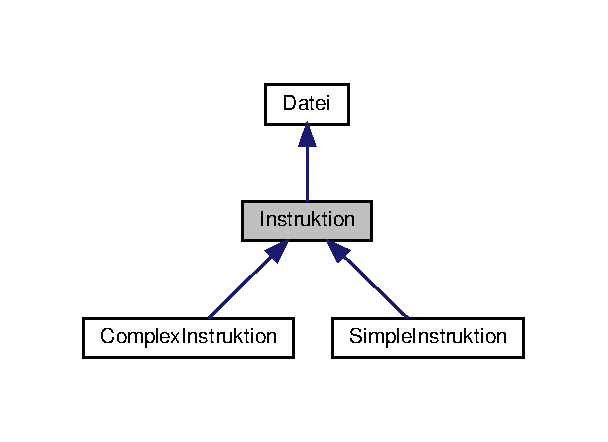
\includegraphics[width=292pt]{class_instruktion__inherit__graph}
\end{center}
\end{figure}


Collaboration diagram for Instruktion\+:
\nopagebreak
\begin{figure}[H]
\begin{center}
\leavevmode
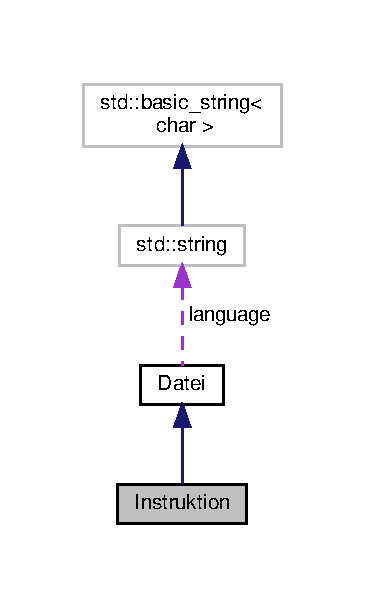
\includegraphics[width=175pt]{class_instruktion__coll__graph}
\end{center}
\end{figure}
\subsection*{Public Member Functions}
\begin{DoxyCompactItemize}
\item 
\mbox{\hyperlink{class_instruktion_a26d54febd2022c7402a22a8b55ba097a}{Instruktion}} (std\+::string str)
\item 
virtual std\+::string \mbox{\hyperlink{class_instruktion_a267ff36e98ec889cceccb2f464c36bc6}{print}} ()=0
\item 
virtual void \mbox{\hyperlink{class_instruktion_ad701f6b5537e5aa8c8c08b81a8946f63}{run}} (\mbox{\hyperlink{class_virtual_machine}{Virtual\+Machine}} \&)=0
\end{DoxyCompactItemize}
\subsection*{Additional Inherited Members}


\subsection{Detailed Description}
Den Basisklasse für die Instruktionentypen. 

Definition at line 13 of file instruction.\+hpp.



\subsection{Constructor \& Destructor Documentation}
\mbox{\Hypertarget{class_instruktion_a26d54febd2022c7402a22a8b55ba097a}\label{class_instruktion_a26d54febd2022c7402a22a8b55ba097a}} 
\index{Instruktion@{Instruktion}!Instruktion@{Instruktion}}
\index{Instruktion@{Instruktion}!Instruktion@{Instruktion}}
\subsubsection{\texorpdfstring{Instruktion()}{Instruktion()}}
{\footnotesize\ttfamily Instruktion\+::\+Instruktion (\begin{DoxyParamCaption}\item[{std\+::string}]{str }\end{DoxyParamCaption})\hspace{0.3cm}{\ttfamily [inline]}}



Definition at line 16 of file instruction.\+hpp.


\begin{DoxyCode}
16 : \mbox{\hyperlink{class_datei_a9a9e1149154603548fdfc889821cf418}{Datei}}(str) \{\}    \textcolor{comment}{/* Konstruktor der Instruktionklasse */}
\end{DoxyCode}


\subsection{Member Function Documentation}
\mbox{\Hypertarget{class_instruktion_a267ff36e98ec889cceccb2f464c36bc6}\label{class_instruktion_a267ff36e98ec889cceccb2f464c36bc6}} 
\index{Instruktion@{Instruktion}!print@{print}}
\index{print@{print}!Instruktion@{Instruktion}}
\subsubsection{\texorpdfstring{print()}{print()}}
{\footnotesize\ttfamily virtual std\+::string Instruktion\+::print (\begin{DoxyParamCaption}{ }\end{DoxyParamCaption})\hspace{0.3cm}{\ttfamily [pure virtual]}}



Implements \mbox{\hyperlink{class_datei_a5dedc9776ebe637f0842300f648d4b17}{Datei}}.



Implemented in \mbox{\hyperlink{class_complex_instruktion_a476d0f6ed0296cd4751543c4be6ca422}{Complex\+Instruktion}}, and \mbox{\hyperlink{class_simple_instruktion_a0533865319bd39a0ecd1db463d488cb8}{Simple\+Instruktion}}.

\mbox{\Hypertarget{class_instruktion_ad701f6b5537e5aa8c8c08b81a8946f63}\label{class_instruktion_ad701f6b5537e5aa8c8c08b81a8946f63}} 
\index{Instruktion@{Instruktion}!run@{run}}
\index{run@{run}!Instruktion@{Instruktion}}
\subsubsection{\texorpdfstring{run()}{run()}}
{\footnotesize\ttfamily virtual void Instruktion\+::run (\begin{DoxyParamCaption}\item[{\mbox{\hyperlink{class_virtual_machine}{Virtual\+Machine}} \&}]{ }\end{DoxyParamCaption})\hspace{0.3cm}{\ttfamily [pure virtual]}}



Implemented in \mbox{\hyperlink{class_complex_instruktion_ab9e037eda3cf53252902f15541a01a21}{Complex\+Instruktion}}, and \mbox{\hyperlink{class_simple_instruktion_a5beecc39bbd465d001c41216ef4d46e7}{Simple\+Instruktion}}.



The documentation for this class was generated from the following file\+:\begin{DoxyCompactItemize}
\item 
src/datei/instruction/\mbox{\hyperlink{instruction_8hpp}{instruction.\+hpp}}\end{DoxyCompactItemize}

\hypertarget{classjson_1_1_j_s_o_n}{}\section{json\+:\+:J\+S\+ON Class Reference}
\label{classjson_1_1_j_s_o_n}\index{json\+::\+J\+S\+ON@{json\+::\+J\+S\+ON}}


{\ttfamily \#include $<$json.\+hpp$>$}



Collaboration diagram for json\+:\+:J\+S\+ON\+:
\nopagebreak
\begin{figure}[H]
\begin{center}
\leavevmode
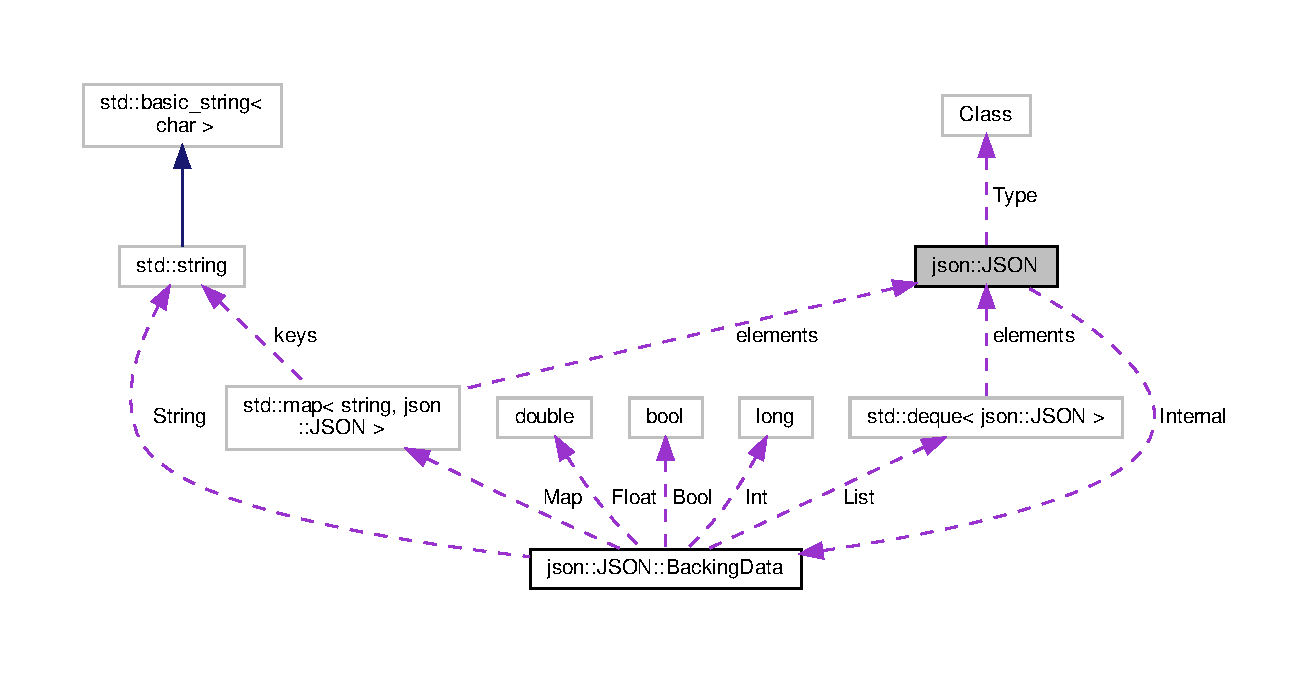
\includegraphics[width=350pt]{classjson_1_1_j_s_o_n__coll__graph}
\end{center}
\end{figure}
\subsection*{Data Structures}
\begin{DoxyCompactItemize}
\item 
union \mbox{\hyperlink{unionjson_1_1_j_s_o_n_1_1_backing_data}{Backing\+Data}}
\item 
class \mbox{\hyperlink{classjson_1_1_j_s_o_n_1_1_j_s_o_n_const_wrapper}{J\+S\+O\+N\+Const\+Wrapper}}
\item 
class \mbox{\hyperlink{classjson_1_1_j_s_o_n_1_1_j_s_o_n_wrapper}{J\+S\+O\+N\+Wrapper}}
\end{DoxyCompactItemize}
\subsection*{Public Types}
\begin{DoxyCompactItemize}
\item 
enum \mbox{\hyperlink{classjson_1_1_j_s_o_n_a762f55df6d407c1af61607ed516ffe07}{Class}} \{ \newline
\mbox{\hyperlink{classjson_1_1_j_s_o_n_a762f55df6d407c1af61607ed516ffe07abbb93ef26e3c101ff11cdd21cab08a94}{Class\+::\+Null}}, 
\mbox{\hyperlink{classjson_1_1_j_s_o_n_a762f55df6d407c1af61607ed516ffe07a497031794414a552435f90151ac3b54b}{Class\+::\+Object}}, 
\mbox{\hyperlink{classjson_1_1_j_s_o_n_a762f55df6d407c1af61607ed516ffe07a4410ec34d9e6c1a68100ca0ce033fb17}{Class\+::\+Array}}, 
\mbox{\hyperlink{classjson_1_1_j_s_o_n_a762f55df6d407c1af61607ed516ffe07a27118326006d3829667a400ad23d5d98}{Class\+::\+String}}, 
\newline
\mbox{\hyperlink{classjson_1_1_j_s_o_n_a762f55df6d407c1af61607ed516ffe07ac8df43648942ec3a9aec140f07f47b7c}{Class\+::\+Floating}}, 
\mbox{\hyperlink{classjson_1_1_j_s_o_n_a762f55df6d407c1af61607ed516ffe07a4ea94552a2bec56a29592359a1b6069e}{Class\+::\+Integral}}, 
\mbox{\hyperlink{classjson_1_1_j_s_o_n_a762f55df6d407c1af61607ed516ffe07a27226c864bac7454a8504f8edb15d95b}{Class\+::\+Boolean}}
 \}
\end{DoxyCompactItemize}
\subsection*{Public Member Functions}
\begin{DoxyCompactItemize}
\item 
\mbox{\hyperlink{classjson_1_1_j_s_o_n_a0334c8643ae2a6cd86020e02643bb20f}{J\+S\+ON}} ()
\item 
\mbox{\hyperlink{classjson_1_1_j_s_o_n_acada0833f1b9fb6974610c031b6eabe7}{J\+S\+ON}} (initializer\+\_\+list$<$ \mbox{\hyperlink{classjson_1_1_j_s_o_n}{J\+S\+ON}} $>$ list)
\item 
\mbox{\hyperlink{classjson_1_1_j_s_o_n_aff59b496d6cebc650355071d32c62edb}{J\+S\+ON}} (\mbox{\hyperlink{classjson_1_1_j_s_o_n}{J\+S\+ON}} \&\&other)
\item 
\mbox{\hyperlink{classjson_1_1_j_s_o_n}{J\+S\+ON}} \& \mbox{\hyperlink{classjson_1_1_j_s_o_n_ab22885428262d4ed0a95c50d5537b13e}{operator=}} (\mbox{\hyperlink{classjson_1_1_j_s_o_n}{J\+S\+ON}} \&\&other)
\item 
\mbox{\hyperlink{classjson_1_1_j_s_o_n_ab147ef429a76d7087fcd7d60ea067405}{J\+S\+ON}} (const \mbox{\hyperlink{classjson_1_1_j_s_o_n}{J\+S\+ON}} \&other)
\item 
\mbox{\hyperlink{classjson_1_1_j_s_o_n}{J\+S\+ON}} \& \mbox{\hyperlink{classjson_1_1_j_s_o_n_ac60d87eca03625eb071fb0c98febbb97}{operator=}} (const \mbox{\hyperlink{classjson_1_1_j_s_o_n}{J\+S\+ON}} \&other)
\item 
\mbox{\hyperlink{classjson_1_1_j_s_o_n_ae67662933b6cc74a8ee6354448874724}{$\sim$\+J\+S\+ON}} ()
\item 
{\footnotesize template$<$typename T $>$ }\\\mbox{\hyperlink{classjson_1_1_j_s_o_n_a8720f6a983f53220b3aa3bb9a461edad}{J\+S\+ON}} (T b, typename enable\+\_\+if$<$ is\+\_\+same$<$ T, bool $>$\+::value $>$\+::type $\ast$=0)
\item 
{\footnotesize template$<$typename T $>$ }\\\mbox{\hyperlink{classjson_1_1_j_s_o_n_af9f080d1de172bc533f9ae49e391f5bf}{J\+S\+ON}} (T i, typename enable\+\_\+if$<$ is\+\_\+integral$<$ T $>$\+::value \&\&!is\+\_\+same$<$ T, bool $>$\+::value $>$\+::type $\ast$=0)
\item 
{\footnotesize template$<$typename T $>$ }\\\mbox{\hyperlink{classjson_1_1_j_s_o_n_aef0009e7c670dfd4a83e39fa1505da55}{J\+S\+ON}} (T f, typename enable\+\_\+if$<$ is\+\_\+floating\+\_\+point$<$ T $>$\+::value $>$\+::type $\ast$=0)
\item 
{\footnotesize template$<$typename T $>$ }\\\mbox{\hyperlink{classjson_1_1_j_s_o_n_af9b32203c09726dd7acbb7e7c11fcd06}{J\+S\+ON}} (T s, typename enable\+\_\+if$<$ is\+\_\+convertible$<$ T, string $>$\+::value $>$\+::type $\ast$=0)
\item 
\mbox{\hyperlink{classjson_1_1_j_s_o_n_ac26eaaa4a2b504b8f7393e73c96e89ec}{J\+S\+ON}} (std\+::nullptr\+\_\+t)
\item 
{\footnotesize template$<$typename T $>$ }\\void \mbox{\hyperlink{classjson_1_1_j_s_o_n_aafb54a2b47ec9bbd7548a60db23fb4cf}{append}} (T arg)
\item 
{\footnotesize template$<$typename T , typename... U$>$ }\\void \mbox{\hyperlink{classjson_1_1_j_s_o_n_ac6a839771cd2c373614e9640eeef6e13}{append}} (T arg, U... args)
\item 
{\footnotesize template$<$typename T $>$ }\\enable\+\_\+if$<$ is\+\_\+same$<$ T, bool $>$\+::value, \mbox{\hyperlink{classjson_1_1_j_s_o_n}{J\+S\+ON}} \& $>$\+::type \mbox{\hyperlink{classjson_1_1_j_s_o_n_a1ee7a8f339bd04d78a4db4aa09cc4e53}{operator=}} (T b)
\item 
{\footnotesize template$<$typename T $>$ }\\enable\+\_\+if$<$ is\+\_\+integral$<$ T $>$\+::value \&\&!is\+\_\+same$<$ T, bool $>$\+::value, \mbox{\hyperlink{classjson_1_1_j_s_o_n}{J\+S\+ON}} \& $>$\+::type \mbox{\hyperlink{classjson_1_1_j_s_o_n_aed9846560a9b7c25b26f684e8d9f32f6}{operator=}} (T i)
\item 
{\footnotesize template$<$typename T $>$ }\\enable\+\_\+if$<$ is\+\_\+floating\+\_\+point$<$ T $>$\+::value, \mbox{\hyperlink{classjson_1_1_j_s_o_n}{J\+S\+ON}} \& $>$\+::type \mbox{\hyperlink{classjson_1_1_j_s_o_n_ac272eeeb42a552c4190a320a4f58a062}{operator=}} (T f)
\item 
{\footnotesize template$<$typename T $>$ }\\enable\+\_\+if$<$ is\+\_\+convertible$<$ T, string $>$\+::value, \mbox{\hyperlink{classjson_1_1_j_s_o_n}{J\+S\+ON}} \& $>$\+::type \mbox{\hyperlink{classjson_1_1_j_s_o_n_ab2dd5163c63d60978a2067a2c1ba50ee}{operator=}} (T s)
\item 
\mbox{\hyperlink{classjson_1_1_j_s_o_n}{J\+S\+ON}} \& \mbox{\hyperlink{classjson_1_1_j_s_o_n_a29c695c67a5b34a3b59af0da3c25d6b1}{operator\mbox{[}$\,$\mbox{]}}} (const string \&key)
\item 
\mbox{\hyperlink{classjson_1_1_j_s_o_n}{J\+S\+ON}} \& \mbox{\hyperlink{classjson_1_1_j_s_o_n_ad590ba3c1aa11aad67e03138ffdc1488}{operator\mbox{[}$\,$\mbox{]}}} (unsigned index)
\item 
\mbox{\hyperlink{classjson_1_1_j_s_o_n}{J\+S\+ON}} \& \mbox{\hyperlink{classjson_1_1_j_s_o_n_a0980eee524bf7442d5f00612984c89c4}{at}} (const string \&key)
\item 
const \mbox{\hyperlink{classjson_1_1_j_s_o_n}{J\+S\+ON}} \& \mbox{\hyperlink{classjson_1_1_j_s_o_n_a7c52c700576374ccab54e006bae06c55}{at}} (const string \&key) const
\item 
\mbox{\hyperlink{classjson_1_1_j_s_o_n}{J\+S\+ON}} \& \mbox{\hyperlink{classjson_1_1_j_s_o_n_ab78dbe91cd205fcc61002f29271ee611}{at}} (unsigned index)
\item 
const \mbox{\hyperlink{classjson_1_1_j_s_o_n}{J\+S\+ON}} \& \mbox{\hyperlink{classjson_1_1_j_s_o_n_a06b051e5e1fc6e6274290042b9a7985d}{at}} (unsigned index) const
\item 
int \mbox{\hyperlink{classjson_1_1_j_s_o_n_a691d475ed40e6352ffaa9af37d664ff3}{length}} () const
\item 
bool \mbox{\hyperlink{classjson_1_1_j_s_o_n_a87283b4ab9833535d16018634421c090}{has\+Key}} (const string \&key) const
\item 
int \mbox{\hyperlink{classjson_1_1_j_s_o_n_af8665d4f94afa84c3e20d52a7184f7ee}{size}} () const
\item 
\mbox{\hyperlink{classjson_1_1_j_s_o_n_a762f55df6d407c1af61607ed516ffe07}{Class}} \mbox{\hyperlink{classjson_1_1_j_s_o_n_a3c91ab49425b2542665a194d6c07ecb6}{J\+S\+O\+N\+Type}} () const
\item 
bool \mbox{\hyperlink{classjson_1_1_j_s_o_n_ab047731707304fc5ac9bd9d6851cd2d9}{Is\+Null}} () const
\begin{DoxyCompactList}\small\item\em Functions for getting primitives from the \mbox{\hyperlink{classjson_1_1_j_s_o_n}{J\+S\+ON}} object. \end{DoxyCompactList}\item 
string \mbox{\hyperlink{classjson_1_1_j_s_o_n_a5f1c7695d59c4652f01cb087eff954f5}{To\+String}} () const
\item 
string \mbox{\hyperlink{classjson_1_1_j_s_o_n_a08f4e57ef30b5dc6881179017e2196d0}{To\+String}} (bool \&ok) const
\item 
double \mbox{\hyperlink{classjson_1_1_j_s_o_n_ae6ff6af2be133af569a9c3dd38f67d93}{To\+Float}} () const
\item 
double \mbox{\hyperlink{classjson_1_1_j_s_o_n_ae913234cd95a1338faf8e198b5a0eb38}{To\+Float}} (bool \&ok) const
\item 
long \mbox{\hyperlink{classjson_1_1_j_s_o_n_a867eb9869140b69428287c98d4f56388}{To\+Int}} () const
\item 
long \mbox{\hyperlink{classjson_1_1_j_s_o_n_a12e5b118ced359fd4a315c95a7486007}{To\+Int}} (bool \&ok) const
\item 
bool \mbox{\hyperlink{classjson_1_1_j_s_o_n_adb9ab4683ee30055912b47220780de16}{To\+Bool}} () const
\item 
bool \mbox{\hyperlink{classjson_1_1_j_s_o_n_aa86f03b8572b13dd768c902da2d83efa}{To\+Bool}} (bool \&ok) const
\item 
\mbox{\hyperlink{classjson_1_1_j_s_o_n_1_1_j_s_o_n_wrapper}{J\+S\+O\+N\+Wrapper}}$<$ map$<$ string, \mbox{\hyperlink{classjson_1_1_j_s_o_n}{J\+S\+ON}} $>$ $>$ \mbox{\hyperlink{classjson_1_1_j_s_o_n_a5e2527751cd1ae28b29e82fd1de15555}{Object\+Range}} ()
\item 
\mbox{\hyperlink{classjson_1_1_j_s_o_n_1_1_j_s_o_n_wrapper}{J\+S\+O\+N\+Wrapper}}$<$ deque$<$ \mbox{\hyperlink{classjson_1_1_j_s_o_n}{J\+S\+ON}} $>$ $>$ \mbox{\hyperlink{classjson_1_1_j_s_o_n_ab26986d77f63734f154da3606423c098}{Array\+Range}} ()
\item 
\mbox{\hyperlink{classjson_1_1_j_s_o_n_1_1_j_s_o_n_const_wrapper}{J\+S\+O\+N\+Const\+Wrapper}}$<$ map$<$ string, \mbox{\hyperlink{classjson_1_1_j_s_o_n}{J\+S\+ON}} $>$ $>$ \mbox{\hyperlink{classjson_1_1_j_s_o_n_a23a72db5a52bca8b080334198bb25041}{Object\+Range}} () const
\item 
\mbox{\hyperlink{classjson_1_1_j_s_o_n_1_1_j_s_o_n_const_wrapper}{J\+S\+O\+N\+Const\+Wrapper}}$<$ deque$<$ \mbox{\hyperlink{classjson_1_1_j_s_o_n}{J\+S\+ON}} $>$ $>$ \mbox{\hyperlink{classjson_1_1_j_s_o_n_a7e57080ed10b2903c792146f81bf90eb}{Array\+Range}} () const
\item 
string \mbox{\hyperlink{classjson_1_1_j_s_o_n_acb99af0df2045a504f6bbc08bf5c4990}{dump}} (int depth=1, string tab=\char`\"{}  \char`\"{}) const
\end{DoxyCompactItemize}
\subsection*{Static Public Member Functions}
\begin{DoxyCompactItemize}
\item 
static \mbox{\hyperlink{classjson_1_1_j_s_o_n}{J\+S\+ON}} \mbox{\hyperlink{classjson_1_1_j_s_o_n_aa679dc348ed9711357c315a461b65957}{Make}} (\mbox{\hyperlink{classjson_1_1_j_s_o_n_a762f55df6d407c1af61607ed516ffe07}{Class}} type)
\item 
static \mbox{\hyperlink{classjson_1_1_j_s_o_n}{J\+S\+ON}} \mbox{\hyperlink{classjson_1_1_j_s_o_n_a799ab1cc68cb6e2a41ec948a9a2ecc37}{Load}} (const string \&)
\end{DoxyCompactItemize}
\subsection*{Private Member Functions}
\begin{DoxyCompactItemize}
\item 
void \mbox{\hyperlink{classjson_1_1_j_s_o_n_a668500208950e48394fc8bfe7c320205}{Set\+Type}} (\mbox{\hyperlink{classjson_1_1_j_s_o_n_a762f55df6d407c1af61607ed516ffe07}{Class}} type)
\item 
void \mbox{\hyperlink{classjson_1_1_j_s_o_n_afefdc8c18c2c40575c2c8463fbd78c67}{Clear\+Internal}} ()
\end{DoxyCompactItemize}
\subsection*{Private Attributes}
\begin{DoxyCompactItemize}
\item 
union \mbox{\hyperlink{unionjson_1_1_j_s_o_n_1_1_backing_data}{json\+::\+J\+S\+O\+N\+::\+Backing\+Data}} \mbox{\hyperlink{classjson_1_1_j_s_o_n_a1e2a064794c3d55c8bb8887fc5734947}{Internal}}
\item 
\mbox{\hyperlink{classjson_1_1_j_s_o_n_a762f55df6d407c1af61607ed516ffe07}{Class}} \mbox{\hyperlink{classjson_1_1_j_s_o_n_a3fa6923afa41bdfe38077fbc0079aaf5}{Type}} = \mbox{\hyperlink{classjson_1_1_j_s_o_n_a762f55df6d407c1af61607ed516ffe07abbb93ef26e3c101ff11cdd21cab08a94}{Class\+::\+Null}}
\end{DoxyCompactItemize}
\subsection*{Friends}
\begin{DoxyCompactItemize}
\item 
std\+::ostream \& \mbox{\hyperlink{classjson_1_1_j_s_o_n_a5513ab67f2660e88d73c75fc83b6945c}{operator$<$$<$}} (std\+::ostream \&, const \mbox{\hyperlink{classjson_1_1_j_s_o_n}{J\+S\+ON}} \&)
\end{DoxyCompactItemize}


\subsection{Detailed Description}


Definition at line 45 of file json.\+hpp.



\subsection{Member Enumeration Documentation}
\mbox{\Hypertarget{classjson_1_1_j_s_o_n_a762f55df6d407c1af61607ed516ffe07}\label{classjson_1_1_j_s_o_n_a762f55df6d407c1af61607ed516ffe07}} 
\index{json\+::\+J\+S\+ON@{json\+::\+J\+S\+ON}!Class@{Class}}
\index{Class@{Class}!json\+::\+J\+S\+ON@{json\+::\+J\+S\+ON}}
\subsubsection{\texorpdfstring{Class}{Class}}
{\footnotesize\ttfamily enum \mbox{\hyperlink{classjson_1_1_j_s_o_n_a762f55df6d407c1af61607ed516ffe07}{json\+::\+J\+S\+O\+N\+::\+Class}}\hspace{0.3cm}{\ttfamily [strong]}}

\begin{DoxyEnumFields}{Enumerator}
\raisebox{\heightof{T}}[0pt][0pt]{\index{Null@{Null}!json\+::\+J\+S\+ON@{json\+::\+J\+S\+ON}}\index{json\+::\+J\+S\+ON@{json\+::\+J\+S\+ON}!Null@{Null}}}\mbox{\Hypertarget{classjson_1_1_j_s_o_n_a762f55df6d407c1af61607ed516ffe07abbb93ef26e3c101ff11cdd21cab08a94}\label{classjson_1_1_j_s_o_n_a762f55df6d407c1af61607ed516ffe07abbb93ef26e3c101ff11cdd21cab08a94}} 
Null&\\
\hline

\raisebox{\heightof{T}}[0pt][0pt]{\index{Object@{Object}!json\+::\+J\+S\+ON@{json\+::\+J\+S\+ON}}\index{json\+::\+J\+S\+ON@{json\+::\+J\+S\+ON}!Object@{Object}}}\mbox{\Hypertarget{classjson_1_1_j_s_o_n_a762f55df6d407c1af61607ed516ffe07a497031794414a552435f90151ac3b54b}\label{classjson_1_1_j_s_o_n_a762f55df6d407c1af61607ed516ffe07a497031794414a552435f90151ac3b54b}} 
Object&\\
\hline

\raisebox{\heightof{T}}[0pt][0pt]{\index{Array@{Array}!json\+::\+J\+S\+ON@{json\+::\+J\+S\+ON}}\index{json\+::\+J\+S\+ON@{json\+::\+J\+S\+ON}!Array@{Array}}}\mbox{\Hypertarget{classjson_1_1_j_s_o_n_a762f55df6d407c1af61607ed516ffe07a4410ec34d9e6c1a68100ca0ce033fb17}\label{classjson_1_1_j_s_o_n_a762f55df6d407c1af61607ed516ffe07a4410ec34d9e6c1a68100ca0ce033fb17}} 
Array&\\
\hline

\raisebox{\heightof{T}}[0pt][0pt]{\index{String@{String}!json\+::\+J\+S\+ON@{json\+::\+J\+S\+ON}}\index{json\+::\+J\+S\+ON@{json\+::\+J\+S\+ON}!String@{String}}}\mbox{\Hypertarget{classjson_1_1_j_s_o_n_a762f55df6d407c1af61607ed516ffe07a27118326006d3829667a400ad23d5d98}\label{classjson_1_1_j_s_o_n_a762f55df6d407c1af61607ed516ffe07a27118326006d3829667a400ad23d5d98}} 
String&\\
\hline

\raisebox{\heightof{T}}[0pt][0pt]{\index{Floating@{Floating}!json\+::\+J\+S\+ON@{json\+::\+J\+S\+ON}}\index{json\+::\+J\+S\+ON@{json\+::\+J\+S\+ON}!Floating@{Floating}}}\mbox{\Hypertarget{classjson_1_1_j_s_o_n_a762f55df6d407c1af61607ed516ffe07ac8df43648942ec3a9aec140f07f47b7c}\label{classjson_1_1_j_s_o_n_a762f55df6d407c1af61607ed516ffe07ac8df43648942ec3a9aec140f07f47b7c}} 
Floating&\\
\hline

\raisebox{\heightof{T}}[0pt][0pt]{\index{Integral@{Integral}!json\+::\+J\+S\+ON@{json\+::\+J\+S\+ON}}\index{json\+::\+J\+S\+ON@{json\+::\+J\+S\+ON}!Integral@{Integral}}}\mbox{\Hypertarget{classjson_1_1_j_s_o_n_a762f55df6d407c1af61607ed516ffe07a4ea94552a2bec56a29592359a1b6069e}\label{classjson_1_1_j_s_o_n_a762f55df6d407c1af61607ed516ffe07a4ea94552a2bec56a29592359a1b6069e}} 
Integral&\\
\hline

\raisebox{\heightof{T}}[0pt][0pt]{\index{Boolean@{Boolean}!json\+::\+J\+S\+ON@{json\+::\+J\+S\+ON}}\index{json\+::\+J\+S\+ON@{json\+::\+J\+S\+ON}!Boolean@{Boolean}}}\mbox{\Hypertarget{classjson_1_1_j_s_o_n_a762f55df6d407c1af61607ed516ffe07a27226c864bac7454a8504f8edb15d95b}\label{classjson_1_1_j_s_o_n_a762f55df6d407c1af61607ed516ffe07a27226c864bac7454a8504f8edb15d95b}} 
Boolean&\\
\hline

\end{DoxyEnumFields}


Definition at line 63 of file json.\+hpp.


\begin{DoxyCode}
63                          \{
64             Null,
65             \mbox{\hyperlink{namespacejson_a7bc7d25f21c18a652a42db29cfdabd06}{Object}},
66             \mbox{\hyperlink{namespacejson_a805054691c80da00fd9129387f834c21}{Array}},
67             String,
68             Floating,
69             Integral,
70             Boolean
71         \};
\end{DoxyCode}


\subsection{Constructor \& Destructor Documentation}
\mbox{\Hypertarget{classjson_1_1_j_s_o_n_a0334c8643ae2a6cd86020e02643bb20f}\label{classjson_1_1_j_s_o_n_a0334c8643ae2a6cd86020e02643bb20f}} 
\index{json\+::\+J\+S\+ON@{json\+::\+J\+S\+ON}!J\+S\+ON@{J\+S\+ON}}
\index{J\+S\+ON@{J\+S\+ON}!json\+::\+J\+S\+ON@{json\+::\+J\+S\+ON}}
\subsubsection{\texorpdfstring{J\+S\+O\+N()}{JSON()}\hspace{0.1cm}{\footnotesize\ttfamily [1/9]}}
{\footnotesize\ttfamily json\+::\+J\+S\+O\+N\+::\+J\+S\+ON (\begin{DoxyParamCaption}{ }\end{DoxyParamCaption})\hspace{0.3cm}{\ttfamily [inline]}}



Definition at line 99 of file json.\+hpp.


\begin{DoxyCode}
99 : \mbox{\hyperlink{classjson_1_1_j_s_o_n_a1e2a064794c3d55c8bb8887fc5734947}{Internal}}(), \mbox{\hyperlink{classjson_1_1_j_s_o_n_a3fa6923afa41bdfe38077fbc0079aaf5}{Type}}( \mbox{\hyperlink{classjson_1_1_j_s_o_n_a762f55df6d407c1af61607ed516ffe07abbb93ef26e3c101ff11cdd21cab08a94}{Class::Null}} )\{\}
\end{DoxyCode}
\mbox{\Hypertarget{classjson_1_1_j_s_o_n_acada0833f1b9fb6974610c031b6eabe7}\label{classjson_1_1_j_s_o_n_acada0833f1b9fb6974610c031b6eabe7}} 
\index{json\+::\+J\+S\+ON@{json\+::\+J\+S\+ON}!J\+S\+ON@{J\+S\+ON}}
\index{J\+S\+ON@{J\+S\+ON}!json\+::\+J\+S\+ON@{json\+::\+J\+S\+ON}}
\subsubsection{\texorpdfstring{J\+S\+O\+N()}{JSON()}\hspace{0.1cm}{\footnotesize\ttfamily [2/9]}}
{\footnotesize\ttfamily json\+::\+J\+S\+O\+N\+::\+J\+S\+ON (\begin{DoxyParamCaption}\item[{initializer\+\_\+list$<$ \mbox{\hyperlink{classjson_1_1_j_s_o_n}{J\+S\+ON}} $>$}]{list }\end{DoxyParamCaption})\hspace{0.3cm}{\ttfamily [inline]}}



Definition at line 101 of file json.\+hpp.



References Object, and Set\+Type().


\begin{DoxyCode}
102             : \mbox{\hyperlink{classjson_1_1_j_s_o_n_a0334c8643ae2a6cd86020e02643bb20f}{JSON}}() 
103         \{
104             \mbox{\hyperlink{classjson_1_1_j_s_o_n_a668500208950e48394fc8bfe7c320205}{SetType}}( \mbox{\hyperlink{classjson_1_1_j_s_o_n_a762f55df6d407c1af61607ed516ffe07a497031794414a552435f90151ac3b54b}{Class::Object}} );
105             \textcolor{keywordflow}{for}( \textcolor{keyword}{auto} i = list.begin(), e = list.end(); i != e; ++i, ++i )
106                 \textcolor{keyword}{operator}[]( i->ToString() ) = *std::next( i );
107         \}
\end{DoxyCode}
Here is the call graph for this function\+:
\nopagebreak
\begin{figure}[H]
\begin{center}
\leavevmode
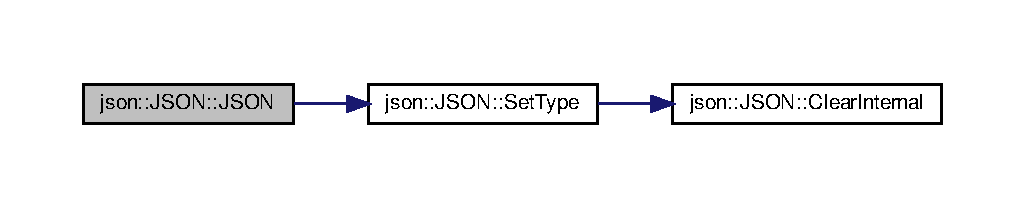
\includegraphics[width=350pt]{classjson_1_1_j_s_o_n_acada0833f1b9fb6974610c031b6eabe7_cgraph}
\end{center}
\end{figure}
\mbox{\Hypertarget{classjson_1_1_j_s_o_n_aff59b496d6cebc650355071d32c62edb}\label{classjson_1_1_j_s_o_n_aff59b496d6cebc650355071d32c62edb}} 
\index{json\+::\+J\+S\+ON@{json\+::\+J\+S\+ON}!J\+S\+ON@{J\+S\+ON}}
\index{J\+S\+ON@{J\+S\+ON}!json\+::\+J\+S\+ON@{json\+::\+J\+S\+ON}}
\subsubsection{\texorpdfstring{J\+S\+O\+N()}{JSON()}\hspace{0.1cm}{\footnotesize\ttfamily [3/9]}}
{\footnotesize\ttfamily json\+::\+J\+S\+O\+N\+::\+J\+S\+ON (\begin{DoxyParamCaption}\item[{\mbox{\hyperlink{classjson_1_1_j_s_o_n}{J\+S\+ON}} \&\&}]{other }\end{DoxyParamCaption})\hspace{0.3cm}{\ttfamily [inline]}}



Definition at line 109 of file json.\+hpp.



References Null.


\begin{DoxyCode}
110             : \mbox{\hyperlink{classjson_1_1_j_s_o_n_a1e2a064794c3d55c8bb8887fc5734947}{Internal}}( other.Internal )
111             , \mbox{\hyperlink{classjson_1_1_j_s_o_n_a3fa6923afa41bdfe38077fbc0079aaf5}{Type}}( other.Type )
112         \{ other.Type = \mbox{\hyperlink{classjson_1_1_j_s_o_n_a762f55df6d407c1af61607ed516ffe07abbb93ef26e3c101ff11cdd21cab08a94}{Class::Null}}; other.Internal.Map = \textcolor{keyword}{nullptr}; \}
\end{DoxyCode}
\mbox{\Hypertarget{classjson_1_1_j_s_o_n_ab147ef429a76d7087fcd7d60ea067405}\label{classjson_1_1_j_s_o_n_ab147ef429a76d7087fcd7d60ea067405}} 
\index{json\+::\+J\+S\+ON@{json\+::\+J\+S\+ON}!J\+S\+ON@{J\+S\+ON}}
\index{J\+S\+ON@{J\+S\+ON}!json\+::\+J\+S\+ON@{json\+::\+J\+S\+ON}}
\subsubsection{\texorpdfstring{J\+S\+O\+N()}{JSON()}\hspace{0.1cm}{\footnotesize\ttfamily [4/9]}}
{\footnotesize\ttfamily json\+::\+J\+S\+O\+N\+::\+J\+S\+ON (\begin{DoxyParamCaption}\item[{const \mbox{\hyperlink{classjson_1_1_j_s_o_n}{J\+S\+ON}} \&}]{other }\end{DoxyParamCaption})\hspace{0.3cm}{\ttfamily [inline]}}



Definition at line 123 of file json.\+hpp.



References Array, Internal, json\+::\+J\+S\+O\+N\+::\+Backing\+Data\+::\+List, json\+::\+J\+S\+O\+N\+::\+Backing\+Data\+::\+Map, Object, json\+::\+J\+S\+O\+N\+::\+Backing\+Data\+::\+String, String, and Type.


\begin{DoxyCode}
123                                   \{
124             \textcolor{keywordflow}{switch}( other.Type ) \{
125             \textcolor{keywordflow}{case} \mbox{\hyperlink{classjson_1_1_j_s_o_n_a762f55df6d407c1af61607ed516ffe07a497031794414a552435f90151ac3b54b}{Class::Object}}:
126                 \mbox{\hyperlink{classjson_1_1_j_s_o_n_a1e2a064794c3d55c8bb8887fc5734947}{Internal}}.\mbox{\hyperlink{unionjson_1_1_j_s_o_n_1_1_backing_data_ab2e19b00745b37d2add157ff3a35c431}{Map}} = 
127                     \textcolor{keyword}{new} map<string,JSON>( other.Internal.Map->begin(),
128                                           other.Internal.Map->end() );
129                 \textcolor{keywordflow}{break};
130             \textcolor{keywordflow}{case} \mbox{\hyperlink{classjson_1_1_j_s_o_n_a762f55df6d407c1af61607ed516ffe07a4410ec34d9e6c1a68100ca0ce033fb17}{Class::Array}}:
131                 \mbox{\hyperlink{classjson_1_1_j_s_o_n_a1e2a064794c3d55c8bb8887fc5734947}{Internal}}.\mbox{\hyperlink{unionjson_1_1_j_s_o_n_1_1_backing_data_ab85f5e7ad21f9f7a5407ab73128a3ebc}{List}} = 
132                     \textcolor{keyword}{new} deque<JSON>( other.Internal.List->begin(),
133                                       other.Internal.List->end() );
134                 \textcolor{keywordflow}{break};
135             \textcolor{keywordflow}{case} \mbox{\hyperlink{classjson_1_1_j_s_o_n_a762f55df6d407c1af61607ed516ffe07a27118326006d3829667a400ad23d5d98}{Class::String}}:
136                 \mbox{\hyperlink{classjson_1_1_j_s_o_n_a1e2a064794c3d55c8bb8887fc5734947}{Internal}}.\mbox{\hyperlink{unionjson_1_1_j_s_o_n_1_1_backing_data_a883c18d113d2e55767a9530f06a9c772}{String}} = 
137                     \textcolor{keyword}{new} string( *other.Internal.String );
138                 \textcolor{keywordflow}{break};
139             \textcolor{keywordflow}{default}:
140                 \mbox{\hyperlink{classjson_1_1_j_s_o_n_a1e2a064794c3d55c8bb8887fc5734947}{Internal}} = other.Internal;
141             \}
142             \mbox{\hyperlink{classjson_1_1_j_s_o_n_a3fa6923afa41bdfe38077fbc0079aaf5}{Type}} = other.Type;
143         \}
\end{DoxyCode}
\mbox{\Hypertarget{classjson_1_1_j_s_o_n_ae67662933b6cc74a8ee6354448874724}\label{classjson_1_1_j_s_o_n_ae67662933b6cc74a8ee6354448874724}} 
\index{json\+::\+J\+S\+ON@{json\+::\+J\+S\+ON}!````~J\+S\+ON@{$\sim$\+J\+S\+ON}}
\index{````~J\+S\+ON@{$\sim$\+J\+S\+ON}!json\+::\+J\+S\+ON@{json\+::\+J\+S\+ON}}
\subsubsection{\texorpdfstring{$\sim$\+J\+S\+O\+N()}{~JSON()}}
{\footnotesize\ttfamily json\+::\+J\+S\+O\+N\+::$\sim$\+J\+S\+ON (\begin{DoxyParamCaption}{ }\end{DoxyParamCaption})\hspace{0.3cm}{\ttfamily [inline]}}



Definition at line 169 of file json.\+hpp.



References Array, Internal, json\+::\+J\+S\+O\+N\+::\+Backing\+Data\+::\+List, json\+::\+J\+S\+O\+N\+::\+Backing\+Data\+::\+Map, Object, json\+::\+J\+S\+O\+N\+::\+Backing\+Data\+::\+String, String, and Type.


\begin{DoxyCode}
169                 \{
170             \textcolor{keywordflow}{switch}( \mbox{\hyperlink{classjson_1_1_j_s_o_n_a3fa6923afa41bdfe38077fbc0079aaf5}{Type}} ) \{
171             \textcolor{keywordflow}{case} \mbox{\hyperlink{classjson_1_1_j_s_o_n_a762f55df6d407c1af61607ed516ffe07a4410ec34d9e6c1a68100ca0ce033fb17}{Class::Array}}:
172                 \textcolor{keyword}{delete} \mbox{\hyperlink{classjson_1_1_j_s_o_n_a1e2a064794c3d55c8bb8887fc5734947}{Internal}}.\mbox{\hyperlink{unionjson_1_1_j_s_o_n_1_1_backing_data_ab85f5e7ad21f9f7a5407ab73128a3ebc}{List}};
173                 \textcolor{keywordflow}{break};
174             \textcolor{keywordflow}{case} \mbox{\hyperlink{classjson_1_1_j_s_o_n_a762f55df6d407c1af61607ed516ffe07a497031794414a552435f90151ac3b54b}{Class::Object}}:
175                 \textcolor{keyword}{delete} \mbox{\hyperlink{classjson_1_1_j_s_o_n_a1e2a064794c3d55c8bb8887fc5734947}{Internal}}.\mbox{\hyperlink{unionjson_1_1_j_s_o_n_1_1_backing_data_ab2e19b00745b37d2add157ff3a35c431}{Map}};
176                 \textcolor{keywordflow}{break};
177             \textcolor{keywordflow}{case} \mbox{\hyperlink{classjson_1_1_j_s_o_n_a762f55df6d407c1af61607ed516ffe07a27118326006d3829667a400ad23d5d98}{Class::String}}:
178                 \textcolor{keyword}{delete} \mbox{\hyperlink{classjson_1_1_j_s_o_n_a1e2a064794c3d55c8bb8887fc5734947}{Internal}}.\mbox{\hyperlink{unionjson_1_1_j_s_o_n_1_1_backing_data_a883c18d113d2e55767a9530f06a9c772}{String}};
179                 \textcolor{keywordflow}{break};
180             \textcolor{keywordflow}{default}:;
181             \}
182         \}
\end{DoxyCode}
\mbox{\Hypertarget{classjson_1_1_j_s_o_n_a8720f6a983f53220b3aa3bb9a461edad}\label{classjson_1_1_j_s_o_n_a8720f6a983f53220b3aa3bb9a461edad}} 
\index{json\+::\+J\+S\+ON@{json\+::\+J\+S\+ON}!J\+S\+ON@{J\+S\+ON}}
\index{J\+S\+ON@{J\+S\+ON}!json\+::\+J\+S\+ON@{json\+::\+J\+S\+ON}}
\subsubsection{\texorpdfstring{J\+S\+O\+N()}{JSON()}\hspace{0.1cm}{\footnotesize\ttfamily [5/9]}}
{\footnotesize\ttfamily template$<$typename T $>$ \\
json\+::\+J\+S\+O\+N\+::\+J\+S\+ON (\begin{DoxyParamCaption}\item[{T}]{b,  }\item[{typename enable\+\_\+if$<$ is\+\_\+same$<$ T, bool $>$\+::value $>$\+::type $\ast$}]{ = {\ttfamily 0} }\end{DoxyParamCaption})\hspace{0.3cm}{\ttfamily [inline]}}



Definition at line 185 of file json.\+hpp.


\begin{DoxyCode}
185 : \mbox{\hyperlink{classjson_1_1_j_s_o_n_a1e2a064794c3d55c8bb8887fc5734947}{Internal}}( b ), \mbox{\hyperlink{classjson_1_1_j_s_o_n_a3fa6923afa41bdfe38077fbc0079aaf5}{Type}}( \mbox{\hyperlink{classjson_1_1_j_s_o_n_a762f55df6d407c1af61607ed516ffe07a27226c864bac7454a8504f8edb15d95b}{Class::Boolean}} )\{\}
\end{DoxyCode}
\mbox{\Hypertarget{classjson_1_1_j_s_o_n_af9f080d1de172bc533f9ae49e391f5bf}\label{classjson_1_1_j_s_o_n_af9f080d1de172bc533f9ae49e391f5bf}} 
\index{json\+::\+J\+S\+ON@{json\+::\+J\+S\+ON}!J\+S\+ON@{J\+S\+ON}}
\index{J\+S\+ON@{J\+S\+ON}!json\+::\+J\+S\+ON@{json\+::\+J\+S\+ON}}
\subsubsection{\texorpdfstring{J\+S\+O\+N()}{JSON()}\hspace{0.1cm}{\footnotesize\ttfamily [6/9]}}
{\footnotesize\ttfamily template$<$typename T $>$ \\
json\+::\+J\+S\+O\+N\+::\+J\+S\+ON (\begin{DoxyParamCaption}\item[{T}]{i,  }\item[{typename enable\+\_\+if$<$ is\+\_\+integral$<$ T $>$\+::value \&\&!is\+\_\+same$<$ T, bool $>$\+::value $>$\+::type $\ast$}]{ = {\ttfamily 0} }\end{DoxyParamCaption})\hspace{0.3cm}{\ttfamily [inline]}}



Definition at line 188 of file json.\+hpp.


\begin{DoxyCode}
188 : \mbox{\hyperlink{classjson_1_1_j_s_o_n_a1e2a064794c3d55c8bb8887fc5734947}{Internal}}( (\textcolor{keywordtype}{long})i ), \mbox{\hyperlink{classjson_1_1_j_s_o_n_a3fa6923afa41bdfe38077fbc0079aaf5}{Type}}( \mbox{\hyperlink{classjson_1_1_j_s_o_n_a762f55df6d407c1af61607ed516ffe07a4ea94552a2bec56a29592359a1b6069e}{Class::Integral}} )\{\}
\end{DoxyCode}
\mbox{\Hypertarget{classjson_1_1_j_s_o_n_aef0009e7c670dfd4a83e39fa1505da55}\label{classjson_1_1_j_s_o_n_aef0009e7c670dfd4a83e39fa1505da55}} 
\index{json\+::\+J\+S\+ON@{json\+::\+J\+S\+ON}!J\+S\+ON@{J\+S\+ON}}
\index{J\+S\+ON@{J\+S\+ON}!json\+::\+J\+S\+ON@{json\+::\+J\+S\+ON}}
\subsubsection{\texorpdfstring{J\+S\+O\+N()}{JSON()}\hspace{0.1cm}{\footnotesize\ttfamily [7/9]}}
{\footnotesize\ttfamily template$<$typename T $>$ \\
json\+::\+J\+S\+O\+N\+::\+J\+S\+ON (\begin{DoxyParamCaption}\item[{T}]{f,  }\item[{typename enable\+\_\+if$<$ is\+\_\+floating\+\_\+point$<$ T $>$\+::value $>$\+::type $\ast$}]{ = {\ttfamily 0} }\end{DoxyParamCaption})\hspace{0.3cm}{\ttfamily [inline]}}



Definition at line 191 of file json.\+hpp.


\begin{DoxyCode}
191 : \mbox{\hyperlink{classjson_1_1_j_s_o_n_a1e2a064794c3d55c8bb8887fc5734947}{Internal}}( (\textcolor{keywordtype}{double})f ), \mbox{\hyperlink{classjson_1_1_j_s_o_n_a3fa6923afa41bdfe38077fbc0079aaf5}{Type}}( \mbox{\hyperlink{classjson_1_1_j_s_o_n_a762f55df6d407c1af61607ed516ffe07ac8df43648942ec3a9aec140f07f47b7c}{Class::Floating}} )\{\}
\end{DoxyCode}
\mbox{\Hypertarget{classjson_1_1_j_s_o_n_af9b32203c09726dd7acbb7e7c11fcd06}\label{classjson_1_1_j_s_o_n_af9b32203c09726dd7acbb7e7c11fcd06}} 
\index{json\+::\+J\+S\+ON@{json\+::\+J\+S\+ON}!J\+S\+ON@{J\+S\+ON}}
\index{J\+S\+ON@{J\+S\+ON}!json\+::\+J\+S\+ON@{json\+::\+J\+S\+ON}}
\subsubsection{\texorpdfstring{J\+S\+O\+N()}{JSON()}\hspace{0.1cm}{\footnotesize\ttfamily [8/9]}}
{\footnotesize\ttfamily template$<$typename T $>$ \\
json\+::\+J\+S\+O\+N\+::\+J\+S\+ON (\begin{DoxyParamCaption}\item[{T}]{s,  }\item[{typename enable\+\_\+if$<$ is\+\_\+convertible$<$ T, string $>$\+::value $>$\+::type $\ast$}]{ = {\ttfamily 0} }\end{DoxyParamCaption})\hspace{0.3cm}{\ttfamily [inline]}}



Definition at line 194 of file json.\+hpp.


\begin{DoxyCode}
194 : \mbox{\hyperlink{classjson_1_1_j_s_o_n_a1e2a064794c3d55c8bb8887fc5734947}{Internal}}( \textcolor{keywordtype}{string}( s ) ), \mbox{\hyperlink{classjson_1_1_j_s_o_n_a3fa6923afa41bdfe38077fbc0079aaf5}{Type}}( \mbox{\hyperlink{classjson_1_1_j_s_o_n_a762f55df6d407c1af61607ed516ffe07a27118326006d3829667a400ad23d5d98}{Class::String}} )\{\}
\end{DoxyCode}
\mbox{\Hypertarget{classjson_1_1_j_s_o_n_ac26eaaa4a2b504b8f7393e73c96e89ec}\label{classjson_1_1_j_s_o_n_ac26eaaa4a2b504b8f7393e73c96e89ec}} 
\index{json\+::\+J\+S\+ON@{json\+::\+J\+S\+ON}!J\+S\+ON@{J\+S\+ON}}
\index{J\+S\+ON@{J\+S\+ON}!json\+::\+J\+S\+ON@{json\+::\+J\+S\+ON}}
\subsubsection{\texorpdfstring{J\+S\+O\+N()}{JSON()}\hspace{0.1cm}{\footnotesize\ttfamily [9/9]}}
{\footnotesize\ttfamily json\+::\+J\+S\+O\+N\+::\+J\+S\+ON (\begin{DoxyParamCaption}\item[{std\+::nullptr\+\_\+t}]{ }\end{DoxyParamCaption})\hspace{0.3cm}{\ttfamily [inline]}}



Definition at line 196 of file json.\+hpp.


\begin{DoxyCode}
196 : \mbox{\hyperlink{classjson_1_1_j_s_o_n_a1e2a064794c3d55c8bb8887fc5734947}{Internal}}(), \mbox{\hyperlink{classjson_1_1_j_s_o_n_a3fa6923afa41bdfe38077fbc0079aaf5}{Type}}( \mbox{\hyperlink{classjson_1_1_j_s_o_n_a762f55df6d407c1af61607ed516ffe07abbb93ef26e3c101ff11cdd21cab08a94}{Class::Null}} )\{\}
\end{DoxyCode}


\subsection{Member Function Documentation}
\mbox{\Hypertarget{classjson_1_1_j_s_o_n_aafb54a2b47ec9bbd7548a60db23fb4cf}\label{classjson_1_1_j_s_o_n_aafb54a2b47ec9bbd7548a60db23fb4cf}} 
\index{json\+::\+J\+S\+ON@{json\+::\+J\+S\+ON}!append@{append}}
\index{append@{append}!json\+::\+J\+S\+ON@{json\+::\+J\+S\+ON}}
\subsubsection{\texorpdfstring{append()}{append()}\hspace{0.1cm}{\footnotesize\ttfamily [1/2]}}
{\footnotesize\ttfamily template$<$typename T $>$ \\
void json\+::\+J\+S\+O\+N\+::append (\begin{DoxyParamCaption}\item[{T}]{arg }\end{DoxyParamCaption})\hspace{0.3cm}{\ttfamily [inline]}}



Definition at line 206 of file json.\+hpp.



References Array, Internal, json\+::\+J\+S\+O\+N\+::\+Backing\+Data\+::\+List, and Set\+Type().



Referenced by append(), and json\+::\+Array().


\begin{DoxyCode}
206                              \{
207             \mbox{\hyperlink{classjson_1_1_j_s_o_n_a668500208950e48394fc8bfe7c320205}{SetType}}( \mbox{\hyperlink{classjson_1_1_j_s_o_n_a762f55df6d407c1af61607ed516ffe07a4410ec34d9e6c1a68100ca0ce033fb17}{Class::Array}} ); \mbox{\hyperlink{classjson_1_1_j_s_o_n_a1e2a064794c3d55c8bb8887fc5734947}{Internal}}.\mbox{\hyperlink{unionjson_1_1_j_s_o_n_1_1_backing_data_ab85f5e7ad21f9f7a5407ab73128a3ebc}{List}}->emplace\_back( arg );
208         \}
\end{DoxyCode}
Here is the call graph for this function\+:
\nopagebreak
\begin{figure}[H]
\begin{center}
\leavevmode
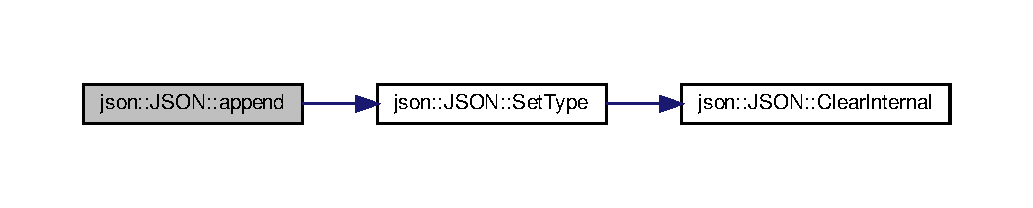
\includegraphics[width=350pt]{classjson_1_1_j_s_o_n_aafb54a2b47ec9bbd7548a60db23fb4cf_cgraph}
\end{center}
\end{figure}
Here is the caller graph for this function\+:
\nopagebreak
\begin{figure}[H]
\begin{center}
\leavevmode
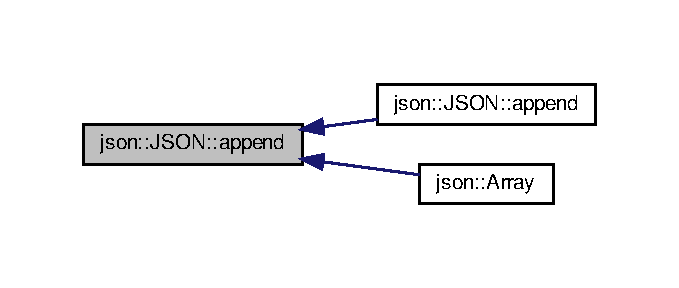
\includegraphics[width=326pt]{classjson_1_1_j_s_o_n_aafb54a2b47ec9bbd7548a60db23fb4cf_icgraph}
\end{center}
\end{figure}
\mbox{\Hypertarget{classjson_1_1_j_s_o_n_ac6a839771cd2c373614e9640eeef6e13}\label{classjson_1_1_j_s_o_n_ac6a839771cd2c373614e9640eeef6e13}} 
\index{json\+::\+J\+S\+ON@{json\+::\+J\+S\+ON}!append@{append}}
\index{append@{append}!json\+::\+J\+S\+ON@{json\+::\+J\+S\+ON}}
\subsubsection{\texorpdfstring{append()}{append()}\hspace{0.1cm}{\footnotesize\ttfamily [2/2]}}
{\footnotesize\ttfamily template$<$typename T , typename... U$>$ \\
void json\+::\+J\+S\+O\+N\+::append (\begin{DoxyParamCaption}\item[{T}]{arg,  }\item[{U...}]{args }\end{DoxyParamCaption})\hspace{0.3cm}{\ttfamily [inline]}}



Definition at line 211 of file json.\+hpp.



References append().


\begin{DoxyCode}
211                                         \{
212             \mbox{\hyperlink{classjson_1_1_j_s_o_n_aafb54a2b47ec9bbd7548a60db23fb4cf}{append}}( arg ); \mbox{\hyperlink{classjson_1_1_j_s_o_n_aafb54a2b47ec9bbd7548a60db23fb4cf}{append}}( args... );
213         \}
\end{DoxyCode}
Here is the call graph for this function\+:
\nopagebreak
\begin{figure}[H]
\begin{center}
\leavevmode
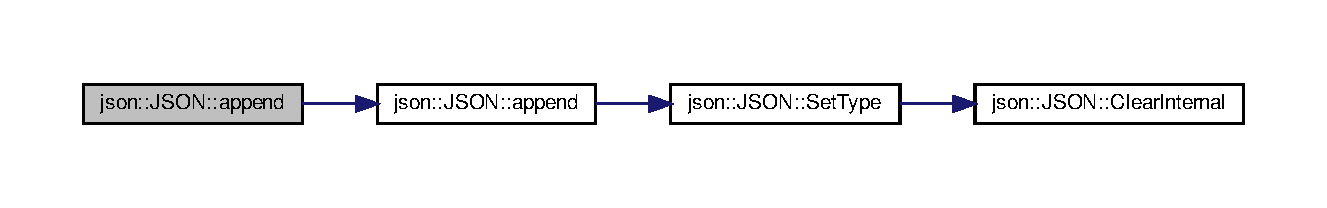
\includegraphics[width=350pt]{classjson_1_1_j_s_o_n_ac6a839771cd2c373614e9640eeef6e13_cgraph}
\end{center}
\end{figure}
\mbox{\Hypertarget{classjson_1_1_j_s_o_n_ab26986d77f63734f154da3606423c098}\label{classjson_1_1_j_s_o_n_ab26986d77f63734f154da3606423c098}} 
\index{json\+::\+J\+S\+ON@{json\+::\+J\+S\+ON}!Array\+Range@{Array\+Range}}
\index{Array\+Range@{Array\+Range}!json\+::\+J\+S\+ON@{json\+::\+J\+S\+ON}}
\subsubsection{\texorpdfstring{Array\+Range()}{ArrayRange()}\hspace{0.1cm}{\footnotesize\ttfamily [1/2]}}
{\footnotesize\ttfamily \mbox{\hyperlink{classjson_1_1_j_s_o_n_1_1_j_s_o_n_wrapper}{J\+S\+O\+N\+Wrapper}}$<$deque$<$\mbox{\hyperlink{classjson_1_1_j_s_o_n}{J\+S\+ON}}$>$ $>$ json\+::\+J\+S\+O\+N\+::\+Array\+Range (\begin{DoxyParamCaption}{ }\end{DoxyParamCaption})\hspace{0.3cm}{\ttfamily [inline]}}



Definition at line 318 of file json.\+hpp.



References Array, Internal, json\+::\+J\+S\+O\+N\+::\+Backing\+Data\+::\+List, and Type.


\begin{DoxyCode}
318                                               \{
319             \textcolor{keywordflow}{if}( \mbox{\hyperlink{classjson_1_1_j_s_o_n_a3fa6923afa41bdfe38077fbc0079aaf5}{Type}} == \mbox{\hyperlink{classjson_1_1_j_s_o_n_a762f55df6d407c1af61607ed516ffe07a4410ec34d9e6c1a68100ca0ce033fb17}{Class::Array}} )
320                 \textcolor{keywordflow}{return} JSONWrapper<deque<JSON>>( \mbox{\hyperlink{classjson_1_1_j_s_o_n_a1e2a064794c3d55c8bb8887fc5734947}{Internal}}.\mbox{\hyperlink{unionjson_1_1_j_s_o_n_1_1_backing_data_ab85f5e7ad21f9f7a5407ab73128a3ebc}{List}} );
321             \textcolor{keywordflow}{return} JSONWrapper<deque<JSON>>( nullptr );
322         \}
\end{DoxyCode}
\mbox{\Hypertarget{classjson_1_1_j_s_o_n_a7e57080ed10b2903c792146f81bf90eb}\label{classjson_1_1_j_s_o_n_a7e57080ed10b2903c792146f81bf90eb}} 
\index{json\+::\+J\+S\+ON@{json\+::\+J\+S\+ON}!Array\+Range@{Array\+Range}}
\index{Array\+Range@{Array\+Range}!json\+::\+J\+S\+ON@{json\+::\+J\+S\+ON}}
\subsubsection{\texorpdfstring{Array\+Range()}{ArrayRange()}\hspace{0.1cm}{\footnotesize\ttfamily [2/2]}}
{\footnotesize\ttfamily \mbox{\hyperlink{classjson_1_1_j_s_o_n_1_1_j_s_o_n_const_wrapper}{J\+S\+O\+N\+Const\+Wrapper}}$<$deque$<$\mbox{\hyperlink{classjson_1_1_j_s_o_n}{J\+S\+ON}}$>$ $>$ json\+::\+J\+S\+O\+N\+::\+Array\+Range (\begin{DoxyParamCaption}{ }\end{DoxyParamCaption}) const\hspace{0.3cm}{\ttfamily [inline]}}



Definition at line 331 of file json.\+hpp.



References Array, Internal, json\+::\+J\+S\+O\+N\+::\+Backing\+Data\+::\+List, and Type.


\begin{DoxyCode}
331                                                          \{ 
332             \textcolor{keywordflow}{if}( \mbox{\hyperlink{classjson_1_1_j_s_o_n_a3fa6923afa41bdfe38077fbc0079aaf5}{Type}} == \mbox{\hyperlink{classjson_1_1_j_s_o_n_a762f55df6d407c1af61607ed516ffe07a4410ec34d9e6c1a68100ca0ce033fb17}{Class::Array}} )
333                 \textcolor{keywordflow}{return} JSONConstWrapper<deque<JSON>>( \mbox{\hyperlink{classjson_1_1_j_s_o_n_a1e2a064794c3d55c8bb8887fc5734947}{Internal}}.\mbox{\hyperlink{unionjson_1_1_j_s_o_n_1_1_backing_data_ab85f5e7ad21f9f7a5407ab73128a3ebc}{List}} );
334             \textcolor{keywordflow}{return} JSONConstWrapper<deque<JSON>>( nullptr );
335         \}
\end{DoxyCode}
\mbox{\Hypertarget{classjson_1_1_j_s_o_n_a0980eee524bf7442d5f00612984c89c4}\label{classjson_1_1_j_s_o_n_a0980eee524bf7442d5f00612984c89c4}} 
\index{json\+::\+J\+S\+ON@{json\+::\+J\+S\+ON}!at@{at}}
\index{at@{at}!json\+::\+J\+S\+ON@{json\+::\+J\+S\+ON}}
\subsubsection{\texorpdfstring{at()}{at()}\hspace{0.1cm}{\footnotesize\ttfamily [1/4]}}
{\footnotesize\ttfamily \mbox{\hyperlink{classjson_1_1_j_s_o_n}{J\+S\+ON}}\& json\+::\+J\+S\+O\+N\+::at (\begin{DoxyParamCaption}\item[{const string \&}]{key }\end{DoxyParamCaption})\hspace{0.3cm}{\ttfamily [inline]}}



Definition at line 245 of file json.\+hpp.



References operator\mbox{[}$\,$\mbox{]}().


\begin{DoxyCode}
245                                       \{
246             \textcolor{keywordflow}{return} \mbox{\hyperlink{classjson_1_1_j_s_o_n_a29c695c67a5b34a3b59af0da3c25d6b1}{operator[]}}( key );
247         \}
\end{DoxyCode}
Here is the call graph for this function\+:
\nopagebreak
\begin{figure}[H]
\begin{center}
\leavevmode
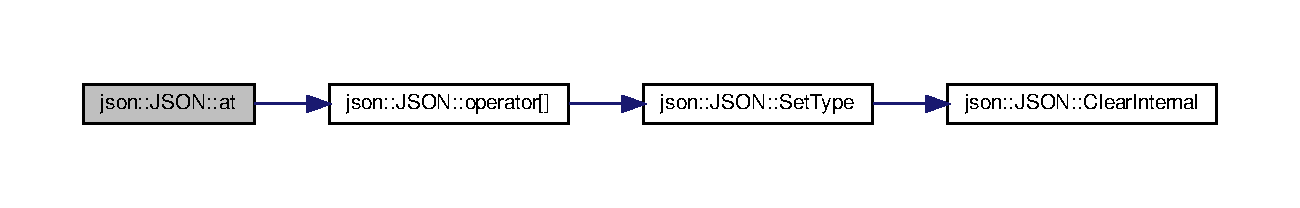
\includegraphics[width=350pt]{classjson_1_1_j_s_o_n_a0980eee524bf7442d5f00612984c89c4_cgraph}
\end{center}
\end{figure}
\mbox{\Hypertarget{classjson_1_1_j_s_o_n_a7c52c700576374ccab54e006bae06c55}\label{classjson_1_1_j_s_o_n_a7c52c700576374ccab54e006bae06c55}} 
\index{json\+::\+J\+S\+ON@{json\+::\+J\+S\+ON}!at@{at}}
\index{at@{at}!json\+::\+J\+S\+ON@{json\+::\+J\+S\+ON}}
\subsubsection{\texorpdfstring{at()}{at()}\hspace{0.1cm}{\footnotesize\ttfamily [2/4]}}
{\footnotesize\ttfamily const \mbox{\hyperlink{classjson_1_1_j_s_o_n}{J\+S\+ON}}\& json\+::\+J\+S\+O\+N\+::at (\begin{DoxyParamCaption}\item[{const string \&}]{key }\end{DoxyParamCaption}) const\hspace{0.3cm}{\ttfamily [inline]}}



Definition at line 249 of file json.\+hpp.



References Internal, and json\+::\+J\+S\+O\+N\+::\+Backing\+Data\+::\+Map.


\begin{DoxyCode}
249                                                   \{
250             \textcolor{keywordflow}{return} \mbox{\hyperlink{classjson_1_1_j_s_o_n_a1e2a064794c3d55c8bb8887fc5734947}{Internal}}.\mbox{\hyperlink{unionjson_1_1_j_s_o_n_1_1_backing_data_ab2e19b00745b37d2add157ff3a35c431}{Map}}->at( key );
251         \}
\end{DoxyCode}
\mbox{\Hypertarget{classjson_1_1_j_s_o_n_ab78dbe91cd205fcc61002f29271ee611}\label{classjson_1_1_j_s_o_n_ab78dbe91cd205fcc61002f29271ee611}} 
\index{json\+::\+J\+S\+ON@{json\+::\+J\+S\+ON}!at@{at}}
\index{at@{at}!json\+::\+J\+S\+ON@{json\+::\+J\+S\+ON}}
\subsubsection{\texorpdfstring{at()}{at()}\hspace{0.1cm}{\footnotesize\ttfamily [3/4]}}
{\footnotesize\ttfamily \mbox{\hyperlink{classjson_1_1_j_s_o_n}{J\+S\+ON}}\& json\+::\+J\+S\+O\+N\+::at (\begin{DoxyParamCaption}\item[{unsigned}]{index }\end{DoxyParamCaption})\hspace{0.3cm}{\ttfamily [inline]}}



Definition at line 253 of file json.\+hpp.



References operator\mbox{[}$\,$\mbox{]}().


\begin{DoxyCode}
253                                    \{
254             \textcolor{keywordflow}{return} \mbox{\hyperlink{classjson_1_1_j_s_o_n_a29c695c67a5b34a3b59af0da3c25d6b1}{operator[]}}( index );
255         \}
\end{DoxyCode}
Here is the call graph for this function\+:
\nopagebreak
\begin{figure}[H]
\begin{center}
\leavevmode
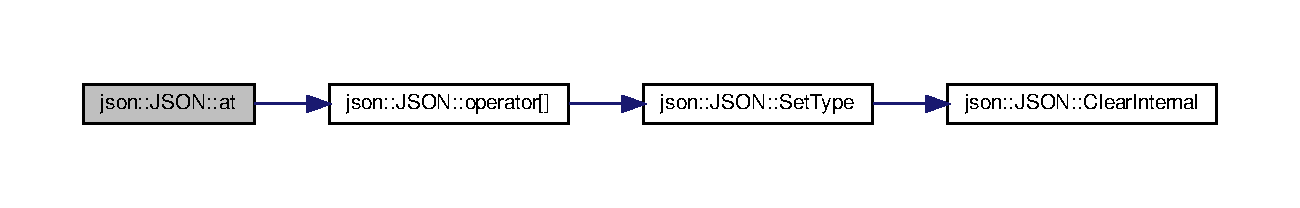
\includegraphics[width=350pt]{classjson_1_1_j_s_o_n_ab78dbe91cd205fcc61002f29271ee611_cgraph}
\end{center}
\end{figure}
\mbox{\Hypertarget{classjson_1_1_j_s_o_n_a06b051e5e1fc6e6274290042b9a7985d}\label{classjson_1_1_j_s_o_n_a06b051e5e1fc6e6274290042b9a7985d}} 
\index{json\+::\+J\+S\+ON@{json\+::\+J\+S\+ON}!at@{at}}
\index{at@{at}!json\+::\+J\+S\+ON@{json\+::\+J\+S\+ON}}
\subsubsection{\texorpdfstring{at()}{at()}\hspace{0.1cm}{\footnotesize\ttfamily [4/4]}}
{\footnotesize\ttfamily const \mbox{\hyperlink{classjson_1_1_j_s_o_n}{J\+S\+ON}}\& json\+::\+J\+S\+O\+N\+::at (\begin{DoxyParamCaption}\item[{unsigned}]{index }\end{DoxyParamCaption}) const\hspace{0.3cm}{\ttfamily [inline]}}



Definition at line 257 of file json.\+hpp.



References Internal, and json\+::\+J\+S\+O\+N\+::\+Backing\+Data\+::\+List.


\begin{DoxyCode}
257                                                \{
258             \textcolor{keywordflow}{return} \mbox{\hyperlink{classjson_1_1_j_s_o_n_a1e2a064794c3d55c8bb8887fc5734947}{Internal}}.\mbox{\hyperlink{unionjson_1_1_j_s_o_n_1_1_backing_data_ab85f5e7ad21f9f7a5407ab73128a3ebc}{List}}->at( index );
259         \}
\end{DoxyCode}
\mbox{\Hypertarget{classjson_1_1_j_s_o_n_afefdc8c18c2c40575c2c8463fbd78c67}\label{classjson_1_1_j_s_o_n_afefdc8c18c2c40575c2c8463fbd78c67}} 
\index{json\+::\+J\+S\+ON@{json\+::\+J\+S\+ON}!Clear\+Internal@{Clear\+Internal}}
\index{Clear\+Internal@{Clear\+Internal}!json\+::\+J\+S\+ON@{json\+::\+J\+S\+ON}}
\subsubsection{\texorpdfstring{Clear\+Internal()}{ClearInternal()}}
{\footnotesize\ttfamily void json\+::\+J\+S\+O\+N\+::\+Clear\+Internal (\begin{DoxyParamCaption}{ }\end{DoxyParamCaption})\hspace{0.3cm}{\ttfamily [inline]}, {\ttfamily [private]}}



Definition at line 407 of file json.\+hpp.



References Array, Internal, json\+::\+J\+S\+O\+N\+::\+Backing\+Data\+::\+List, json\+::\+J\+S\+O\+N\+::\+Backing\+Data\+::\+Map, Object, json\+::\+J\+S\+O\+N\+::\+Backing\+Data\+::\+String, String, and Type.



Referenced by operator=(), and Set\+Type().


\begin{DoxyCode}
407                            \{
408         \textcolor{keywordflow}{switch}( \mbox{\hyperlink{classjson_1_1_j_s_o_n_a3fa6923afa41bdfe38077fbc0079aaf5}{Type}} ) \{
409           \textcolor{keywordflow}{case} \mbox{\hyperlink{classjson_1_1_j_s_o_n_a762f55df6d407c1af61607ed516ffe07a497031794414a552435f90151ac3b54b}{Class::Object}}: \textcolor{keyword}{delete} \mbox{\hyperlink{classjson_1_1_j_s_o_n_a1e2a064794c3d55c8bb8887fc5734947}{Internal}}.\mbox{\hyperlink{unionjson_1_1_j_s_o_n_1_1_backing_data_ab2e19b00745b37d2add157ff3a35c431}{Map}};    \textcolor{keywordflow}{break};
410           \textcolor{keywordflow}{case} \mbox{\hyperlink{classjson_1_1_j_s_o_n_a762f55df6d407c1af61607ed516ffe07a4410ec34d9e6c1a68100ca0ce033fb17}{Class::Array}}:  \textcolor{keyword}{delete} \mbox{\hyperlink{classjson_1_1_j_s_o_n_a1e2a064794c3d55c8bb8887fc5734947}{Internal}}.\mbox{\hyperlink{unionjson_1_1_j_s_o_n_1_1_backing_data_ab85f5e7ad21f9f7a5407ab73128a3ebc}{List}};   \textcolor{keywordflow}{break};
411           \textcolor{keywordflow}{case} \mbox{\hyperlink{classjson_1_1_j_s_o_n_a762f55df6d407c1af61607ed516ffe07a27118326006d3829667a400ad23d5d98}{Class::String}}: \textcolor{keyword}{delete} \mbox{\hyperlink{classjson_1_1_j_s_o_n_a1e2a064794c3d55c8bb8887fc5734947}{Internal}}.\mbox{\hyperlink{unionjson_1_1_j_s_o_n_1_1_backing_data_a883c18d113d2e55767a9530f06a9c772}{String}}; \textcolor{keywordflow}{break};
412           \textcolor{keywordflow}{default}:;
413         \}
414       \}
\end{DoxyCode}
Here is the caller graph for this function\+:
\nopagebreak
\begin{figure}[H]
\begin{center}
\leavevmode
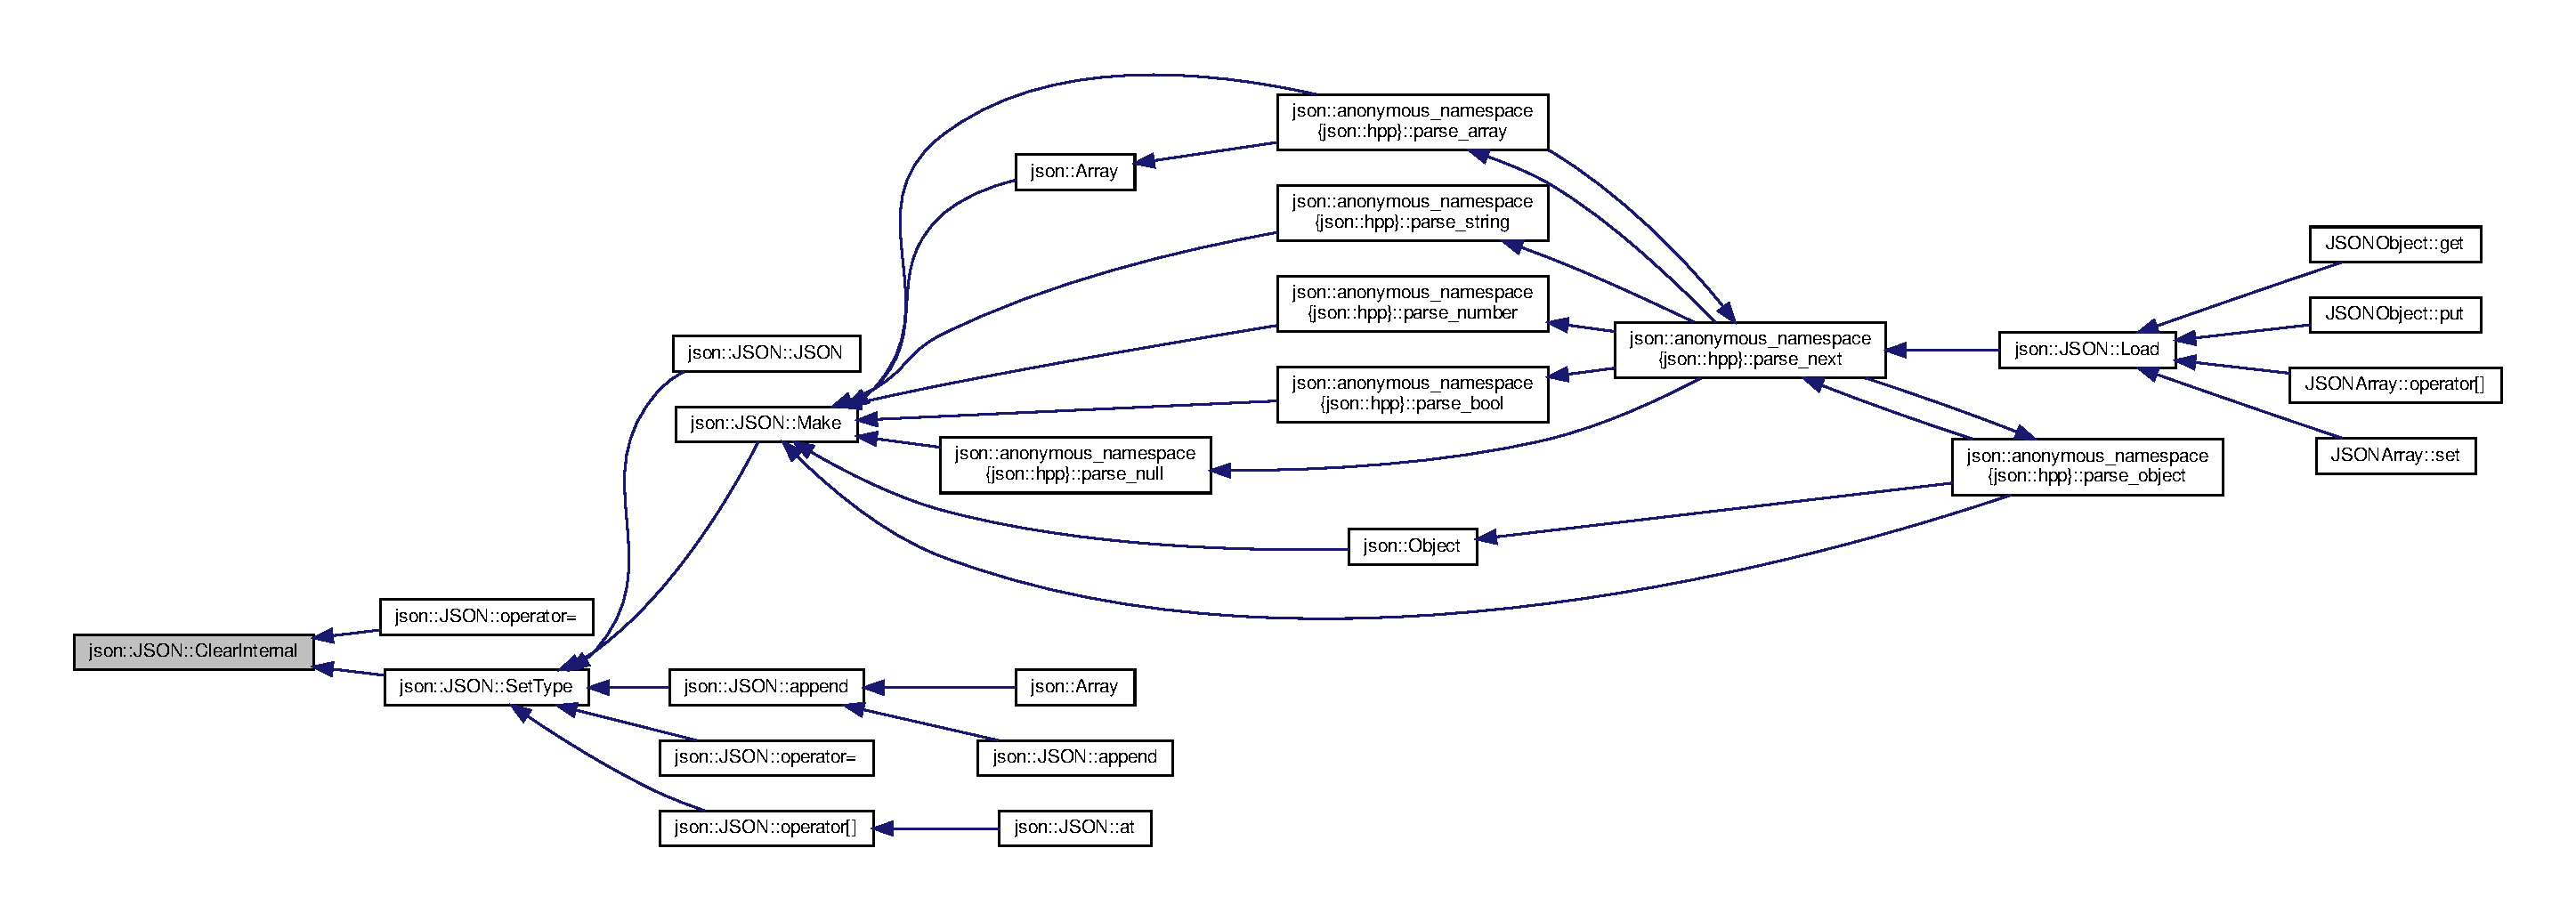
\includegraphics[width=350pt]{classjson_1_1_j_s_o_n_afefdc8c18c2c40575c2c8463fbd78c67_icgraph}
\end{center}
\end{figure}
\mbox{\Hypertarget{classjson_1_1_j_s_o_n_acb99af0df2045a504f6bbc08bf5c4990}\label{classjson_1_1_j_s_o_n_acb99af0df2045a504f6bbc08bf5c4990}} 
\index{json\+::\+J\+S\+ON@{json\+::\+J\+S\+ON}!dump@{dump}}
\index{dump@{dump}!json\+::\+J\+S\+ON@{json\+::\+J\+S\+ON}}
\subsubsection{\texorpdfstring{dump()}{dump()}}
{\footnotesize\ttfamily string json\+::\+J\+S\+O\+N\+::dump (\begin{DoxyParamCaption}\item[{int}]{depth = {\ttfamily 1},  }\item[{string}]{tab = {\ttfamily \char`\"{}~~\char`\"{}} }\end{DoxyParamCaption}) const\hspace{0.3cm}{\ttfamily [inline]}}



Definition at line 337 of file json.\+hpp.



References Array, json\+::\+J\+S\+O\+N\+::\+Backing\+Data\+::\+Bool, Boolean, json\+::\+J\+S\+O\+N\+::\+Backing\+Data\+::\+Float, Floating, json\+::\+J\+S\+O\+N\+::\+Backing\+Data\+::\+Int, Integral, Internal, json\+::anonymous\+\_\+namespace\{json.\+hpp\}\+::json\+\_\+escape(), json\+::\+J\+S\+O\+N\+::\+Backing\+Data\+::\+List, json\+::\+J\+S\+O\+N\+::\+Backing\+Data\+::\+Map, Null, Object, json\+::\+J\+S\+O\+N\+::\+Backing\+Data\+::\+String, String, and Type.



Referenced by J\+S\+O\+N\+Object\+::put(), and J\+S\+O\+N\+Array\+::set().


\begin{DoxyCode}
337                                                              \{
338             \textcolor{keywordtype}{string} pad = \textcolor{stringliteral}{""};
339             \textcolor{keywordflow}{for}( \textcolor{keywordtype}{int} i = 0; i < depth; ++i, pad += tab );
340 
341             \textcolor{keywordflow}{switch}( \mbox{\hyperlink{classjson_1_1_j_s_o_n_a3fa6923afa41bdfe38077fbc0079aaf5}{Type}} ) \{
342                 \textcolor{keywordflow}{case} \mbox{\hyperlink{classjson_1_1_j_s_o_n_a762f55df6d407c1af61607ed516ffe07abbb93ef26e3c101ff11cdd21cab08a94}{Class::Null}}:
343                     \textcolor{keywordflow}{return} \textcolor{stringliteral}{"null"};
344                 \textcolor{keywordflow}{case} \mbox{\hyperlink{classjson_1_1_j_s_o_n_a762f55df6d407c1af61607ed516ffe07a497031794414a552435f90151ac3b54b}{Class::Object}}: \{
345                     \textcolor{keywordtype}{string} s = \textcolor{stringliteral}{"\{\(\backslash\)n"};
346                     \textcolor{keywordtype}{bool} skip = \textcolor{keyword}{true};
347                     \textcolor{keywordflow}{for}( \textcolor{keyword}{auto} &p : *\mbox{\hyperlink{classjson_1_1_j_s_o_n_a1e2a064794c3d55c8bb8887fc5734947}{Internal}}.\mbox{\hyperlink{unionjson_1_1_j_s_o_n_1_1_backing_data_ab2e19b00745b37d2add157ff3a35c431}{Map}} ) \{
348                         \textcolor{keywordflow}{if}( !skip ) s += \textcolor{stringliteral}{",\(\backslash\)n"};
349                         s += ( pad + \textcolor{stringliteral}{""} + p.first + \textcolor{stringliteral}{" : "} + p.second.dump( depth + 1, tab ) );
350                         skip = \textcolor{keyword}{false};
351                     \}
352                     s += ( \textcolor{stringliteral}{"\(\backslash\)n"} + pad.erase( 0, 2 ) + \textcolor{stringliteral}{"\}"} ) ;
353                     \textcolor{keywordflow}{return} s;
354                 \}
355                 \textcolor{keywordflow}{case} \mbox{\hyperlink{classjson_1_1_j_s_o_n_a762f55df6d407c1af61607ed516ffe07a4410ec34d9e6c1a68100ca0ce033fb17}{Class::Array}}: \{
356                     \textcolor{keywordtype}{string} s = \textcolor{stringliteral}{"["};
357                     \textcolor{keywordtype}{bool} skip = \textcolor{keyword}{true};
358                     \textcolor{keywordflow}{for}( \textcolor{keyword}{auto} &p : *\mbox{\hyperlink{classjson_1_1_j_s_o_n_a1e2a064794c3d55c8bb8887fc5734947}{Internal}}.\mbox{\hyperlink{unionjson_1_1_j_s_o_n_1_1_backing_data_ab85f5e7ad21f9f7a5407ab73128a3ebc}{List}} ) \{
359                         \textcolor{keywordflow}{if}( !skip ) s += \textcolor{stringliteral}{", "};
360                         s += p.dump( depth + 1, tab );
361                         skip = \textcolor{keyword}{false};
362                     \}
363                     s += \textcolor{stringliteral}{"]"};
364                     \textcolor{keywordflow}{return} s;
365                 \}
366                 \textcolor{keywordflow}{case} \mbox{\hyperlink{classjson_1_1_j_s_o_n_a762f55df6d407c1af61607ed516ffe07a27118326006d3829667a400ad23d5d98}{Class::String}}:
367                     \textcolor{keywordflow}{return} \textcolor{stringliteral}{""} + \mbox{\hyperlink{namespacejson_1_1anonymous__namespace_02json_8hpp_03_a623a6fca4cd1735d2bf3d081b875a350}{json\_escape}}( *\mbox{\hyperlink{classjson_1_1_j_s_o_n_a1e2a064794c3d55c8bb8887fc5734947}{Internal}}.\mbox{\hyperlink{unionjson_1_1_j_s_o_n_1_1_backing_data_a883c18d113d2e55767a9530f06a9c772}{String}} ) + \textcolor{stringliteral}{""};
368                 \textcolor{keywordflow}{case} \mbox{\hyperlink{classjson_1_1_j_s_o_n_a762f55df6d407c1af61607ed516ffe07ac8df43648942ec3a9aec140f07f47b7c}{Class::Floating}}:
369                     \textcolor{keywordflow}{return} std::to\_string( \mbox{\hyperlink{classjson_1_1_j_s_o_n_a1e2a064794c3d55c8bb8887fc5734947}{Internal}}.\mbox{\hyperlink{unionjson_1_1_j_s_o_n_1_1_backing_data_aac4950afa6b9205bb367a33de47faa5c}{Float}} );
370                 \textcolor{keywordflow}{case} \mbox{\hyperlink{classjson_1_1_j_s_o_n_a762f55df6d407c1af61607ed516ffe07a4ea94552a2bec56a29592359a1b6069e}{Class::Integral}}:
371                     \textcolor{keywordflow}{return} std::to\_string( \mbox{\hyperlink{classjson_1_1_j_s_o_n_a1e2a064794c3d55c8bb8887fc5734947}{Internal}}.\mbox{\hyperlink{unionjson_1_1_j_s_o_n_1_1_backing_data_a0d80815a70ff5bb9345f75de79ec81c3}{Int}} );
372                 \textcolor{keywordflow}{case} \mbox{\hyperlink{classjson_1_1_j_s_o_n_a762f55df6d407c1af61607ed516ffe07a27226c864bac7454a8504f8edb15d95b}{Class::Boolean}}:
373                     \textcolor{keywordflow}{return} \mbox{\hyperlink{classjson_1_1_j_s_o_n_a1e2a064794c3d55c8bb8887fc5734947}{Internal}}.\mbox{\hyperlink{unionjson_1_1_j_s_o_n_1_1_backing_data_a0659fafaedb7de535ae3e79e4ff4688c}{Bool}} ? \textcolor{stringliteral}{"true"} : \textcolor{stringliteral}{"false"};
374                 \textcolor{keywordflow}{default}:
375                     \textcolor{keywordflow}{return} \textcolor{stringliteral}{""};
376             \}
377             \textcolor{keywordflow}{return} \textcolor{stringliteral}{""};
378         \}
\end{DoxyCode}
Here is the call graph for this function\+:
\nopagebreak
\begin{figure}[H]
\begin{center}
\leavevmode
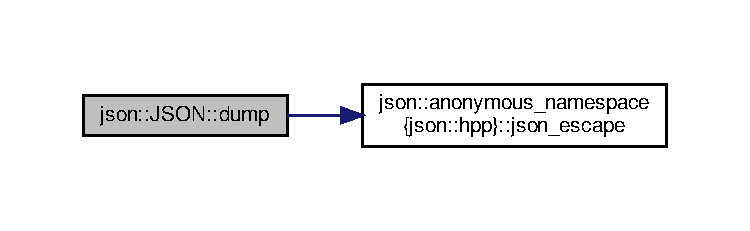
\includegraphics[width=350pt]{classjson_1_1_j_s_o_n_acb99af0df2045a504f6bbc08bf5c4990_cgraph}
\end{center}
\end{figure}
Here is the caller graph for this function\+:
\nopagebreak
\begin{figure}[H]
\begin{center}
\leavevmode
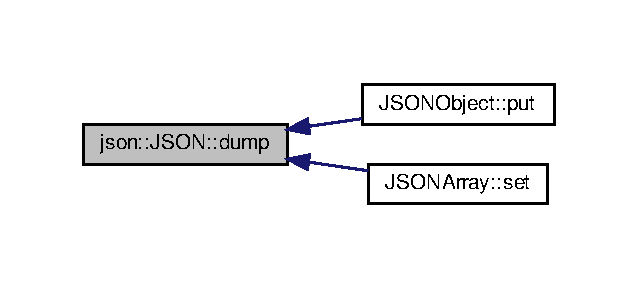
\includegraphics[width=306pt]{classjson_1_1_j_s_o_n_acb99af0df2045a504f6bbc08bf5c4990_icgraph}
\end{center}
\end{figure}
\mbox{\Hypertarget{classjson_1_1_j_s_o_n_a87283b4ab9833535d16018634421c090}\label{classjson_1_1_j_s_o_n_a87283b4ab9833535d16018634421c090}} 
\index{json\+::\+J\+S\+ON@{json\+::\+J\+S\+ON}!has\+Key@{has\+Key}}
\index{has\+Key@{has\+Key}!json\+::\+J\+S\+ON@{json\+::\+J\+S\+ON}}
\subsubsection{\texorpdfstring{has\+Key()}{hasKey()}}
{\footnotesize\ttfamily bool json\+::\+J\+S\+O\+N\+::has\+Key (\begin{DoxyParamCaption}\item[{const string \&}]{key }\end{DoxyParamCaption}) const\hspace{0.3cm}{\ttfamily [inline]}}



Definition at line 268 of file json.\+hpp.



References Internal, json\+::\+J\+S\+O\+N\+::\+Backing\+Data\+::\+Map, Object, and Type.


\begin{DoxyCode}
268                                                \{
269             \textcolor{keywordflow}{if}( \mbox{\hyperlink{classjson_1_1_j_s_o_n_a3fa6923afa41bdfe38077fbc0079aaf5}{Type}} == \mbox{\hyperlink{classjson_1_1_j_s_o_n_a762f55df6d407c1af61607ed516ffe07a497031794414a552435f90151ac3b54b}{Class::Object}} )
270                 \textcolor{keywordflow}{return} \mbox{\hyperlink{classjson_1_1_j_s_o_n_a1e2a064794c3d55c8bb8887fc5734947}{Internal}}.\mbox{\hyperlink{unionjson_1_1_j_s_o_n_1_1_backing_data_ab2e19b00745b37d2add157ff3a35c431}{Map}}->find( key ) != \mbox{\hyperlink{classjson_1_1_j_s_o_n_a1e2a064794c3d55c8bb8887fc5734947}{Internal}}.
      \mbox{\hyperlink{unionjson_1_1_j_s_o_n_1_1_backing_data_ab2e19b00745b37d2add157ff3a35c431}{Map}}->end();
271             \textcolor{keywordflow}{return} \textcolor{keyword}{false};
272         \}
\end{DoxyCode}
\mbox{\Hypertarget{classjson_1_1_j_s_o_n_ab047731707304fc5ac9bd9d6851cd2d9}\label{classjson_1_1_j_s_o_n_ab047731707304fc5ac9bd9d6851cd2d9}} 
\index{json\+::\+J\+S\+ON@{json\+::\+J\+S\+ON}!Is\+Null@{Is\+Null}}
\index{Is\+Null@{Is\+Null}!json\+::\+J\+S\+ON@{json\+::\+J\+S\+ON}}
\subsubsection{\texorpdfstring{Is\+Null()}{IsNull()}}
{\footnotesize\ttfamily bool json\+::\+J\+S\+O\+N\+::\+Is\+Null (\begin{DoxyParamCaption}{ }\end{DoxyParamCaption}) const\hspace{0.3cm}{\ttfamily [inline]}}



Functions for getting primitives from the \mbox{\hyperlink{classjson_1_1_j_s_o_n}{J\+S\+ON}} object. 



Definition at line 286 of file json.\+hpp.



References Null, and Type.


\begin{DoxyCode}
286 \{ \textcolor{keywordflow}{return} \mbox{\hyperlink{classjson_1_1_j_s_o_n_a3fa6923afa41bdfe38077fbc0079aaf5}{Type}} == \mbox{\hyperlink{classjson_1_1_j_s_o_n_a762f55df6d407c1af61607ed516ffe07abbb93ef26e3c101ff11cdd21cab08a94}{Class::Null}}; \}
\end{DoxyCode}
\mbox{\Hypertarget{classjson_1_1_j_s_o_n_a3c91ab49425b2542665a194d6c07ecb6}\label{classjson_1_1_j_s_o_n_a3c91ab49425b2542665a194d6c07ecb6}} 
\index{json\+::\+J\+S\+ON@{json\+::\+J\+S\+ON}!J\+S\+O\+N\+Type@{J\+S\+O\+N\+Type}}
\index{J\+S\+O\+N\+Type@{J\+S\+O\+N\+Type}!json\+::\+J\+S\+ON@{json\+::\+J\+S\+ON}}
\subsubsection{\texorpdfstring{J\+S\+O\+N\+Type()}{JSONType()}}
{\footnotesize\ttfamily \mbox{\hyperlink{classjson_1_1_j_s_o_n_a762f55df6d407c1af61607ed516ffe07}{Class}} json\+::\+J\+S\+O\+N\+::\+J\+S\+O\+N\+Type (\begin{DoxyParamCaption}{ }\end{DoxyParamCaption}) const\hspace{0.3cm}{\ttfamily [inline]}}



Definition at line 283 of file json.\+hpp.



References Type.


\begin{DoxyCode}
283 \{ \textcolor{keywordflow}{return} \mbox{\hyperlink{classjson_1_1_j_s_o_n_a3fa6923afa41bdfe38077fbc0079aaf5}{Type}}; \}
\end{DoxyCode}
\mbox{\Hypertarget{classjson_1_1_j_s_o_n_a691d475ed40e6352ffaa9af37d664ff3}\label{classjson_1_1_j_s_o_n_a691d475ed40e6352ffaa9af37d664ff3}} 
\index{json\+::\+J\+S\+ON@{json\+::\+J\+S\+ON}!length@{length}}
\index{length@{length}!json\+::\+J\+S\+ON@{json\+::\+J\+S\+ON}}
\subsubsection{\texorpdfstring{length()}{length()}}
{\footnotesize\ttfamily int json\+::\+J\+S\+O\+N\+::length (\begin{DoxyParamCaption}{ }\end{DoxyParamCaption}) const\hspace{0.3cm}{\ttfamily [inline]}}



Definition at line 261 of file json.\+hpp.



References Array, Internal, json\+::\+J\+S\+O\+N\+::\+Backing\+Data\+::\+List, and Type.


\begin{DoxyCode}
261                            \{
262             \textcolor{keywordflow}{if}( \mbox{\hyperlink{classjson_1_1_j_s_o_n_a3fa6923afa41bdfe38077fbc0079aaf5}{Type}} == \mbox{\hyperlink{classjson_1_1_j_s_o_n_a762f55df6d407c1af61607ed516ffe07a4410ec34d9e6c1a68100ca0ce033fb17}{Class::Array}} )
263                 \textcolor{keywordflow}{return} \mbox{\hyperlink{classjson_1_1_j_s_o_n_a1e2a064794c3d55c8bb8887fc5734947}{Internal}}.\mbox{\hyperlink{unionjson_1_1_j_s_o_n_1_1_backing_data_ab85f5e7ad21f9f7a5407ab73128a3ebc}{List}}->size();
264             \textcolor{keywordflow}{else}
265                 \textcolor{keywordflow}{return} -1;
266         \}
\end{DoxyCode}
\mbox{\Hypertarget{classjson_1_1_j_s_o_n_a799ab1cc68cb6e2a41ec948a9a2ecc37}\label{classjson_1_1_j_s_o_n_a799ab1cc68cb6e2a41ec948a9a2ecc37}} 
\index{json\+::\+J\+S\+ON@{json\+::\+J\+S\+ON}!Load@{Load}}
\index{Load@{Load}!json\+::\+J\+S\+ON@{json\+::\+J\+S\+ON}}
\subsubsection{\texorpdfstring{Load()}{Load()}}
{\footnotesize\ttfamily \mbox{\hyperlink{classjson_1_1_j_s_o_n}{J\+S\+ON}} J\+S\+O\+N\+::\+Load (\begin{DoxyParamCaption}\item[{const string \&}]{str }\end{DoxyParamCaption})\hspace{0.3cm}{\ttfamily [inline]}, {\ttfamily [static]}}



Definition at line 644 of file json.\+hpp.



References json\+::anonymous\+\_\+namespace\{json.\+hpp\}\+::parse\+\_\+next().



Referenced by J\+S\+O\+N\+Object\+::get(), J\+S\+O\+N\+Array\+::operator\mbox{[}$\,$\mbox{]}(), J\+S\+O\+N\+Object\+::put(), and J\+S\+O\+N\+Array\+::set().


\begin{DoxyCode}
644                                           \{
645     \textcolor{keywordtype}{size\_t} offset = 0;
646     \textcolor{keywordflow}{return} std::move( \mbox{\hyperlink{namespacejson_1_1anonymous__namespace_02json_8hpp_03_acd55b945d1583038db8633516df7cf3f}{parse\_next}}( str, offset ) );
647 \}
\end{DoxyCode}
Here is the call graph for this function\+:
\nopagebreak
\begin{figure}[H]
\begin{center}
\leavevmode
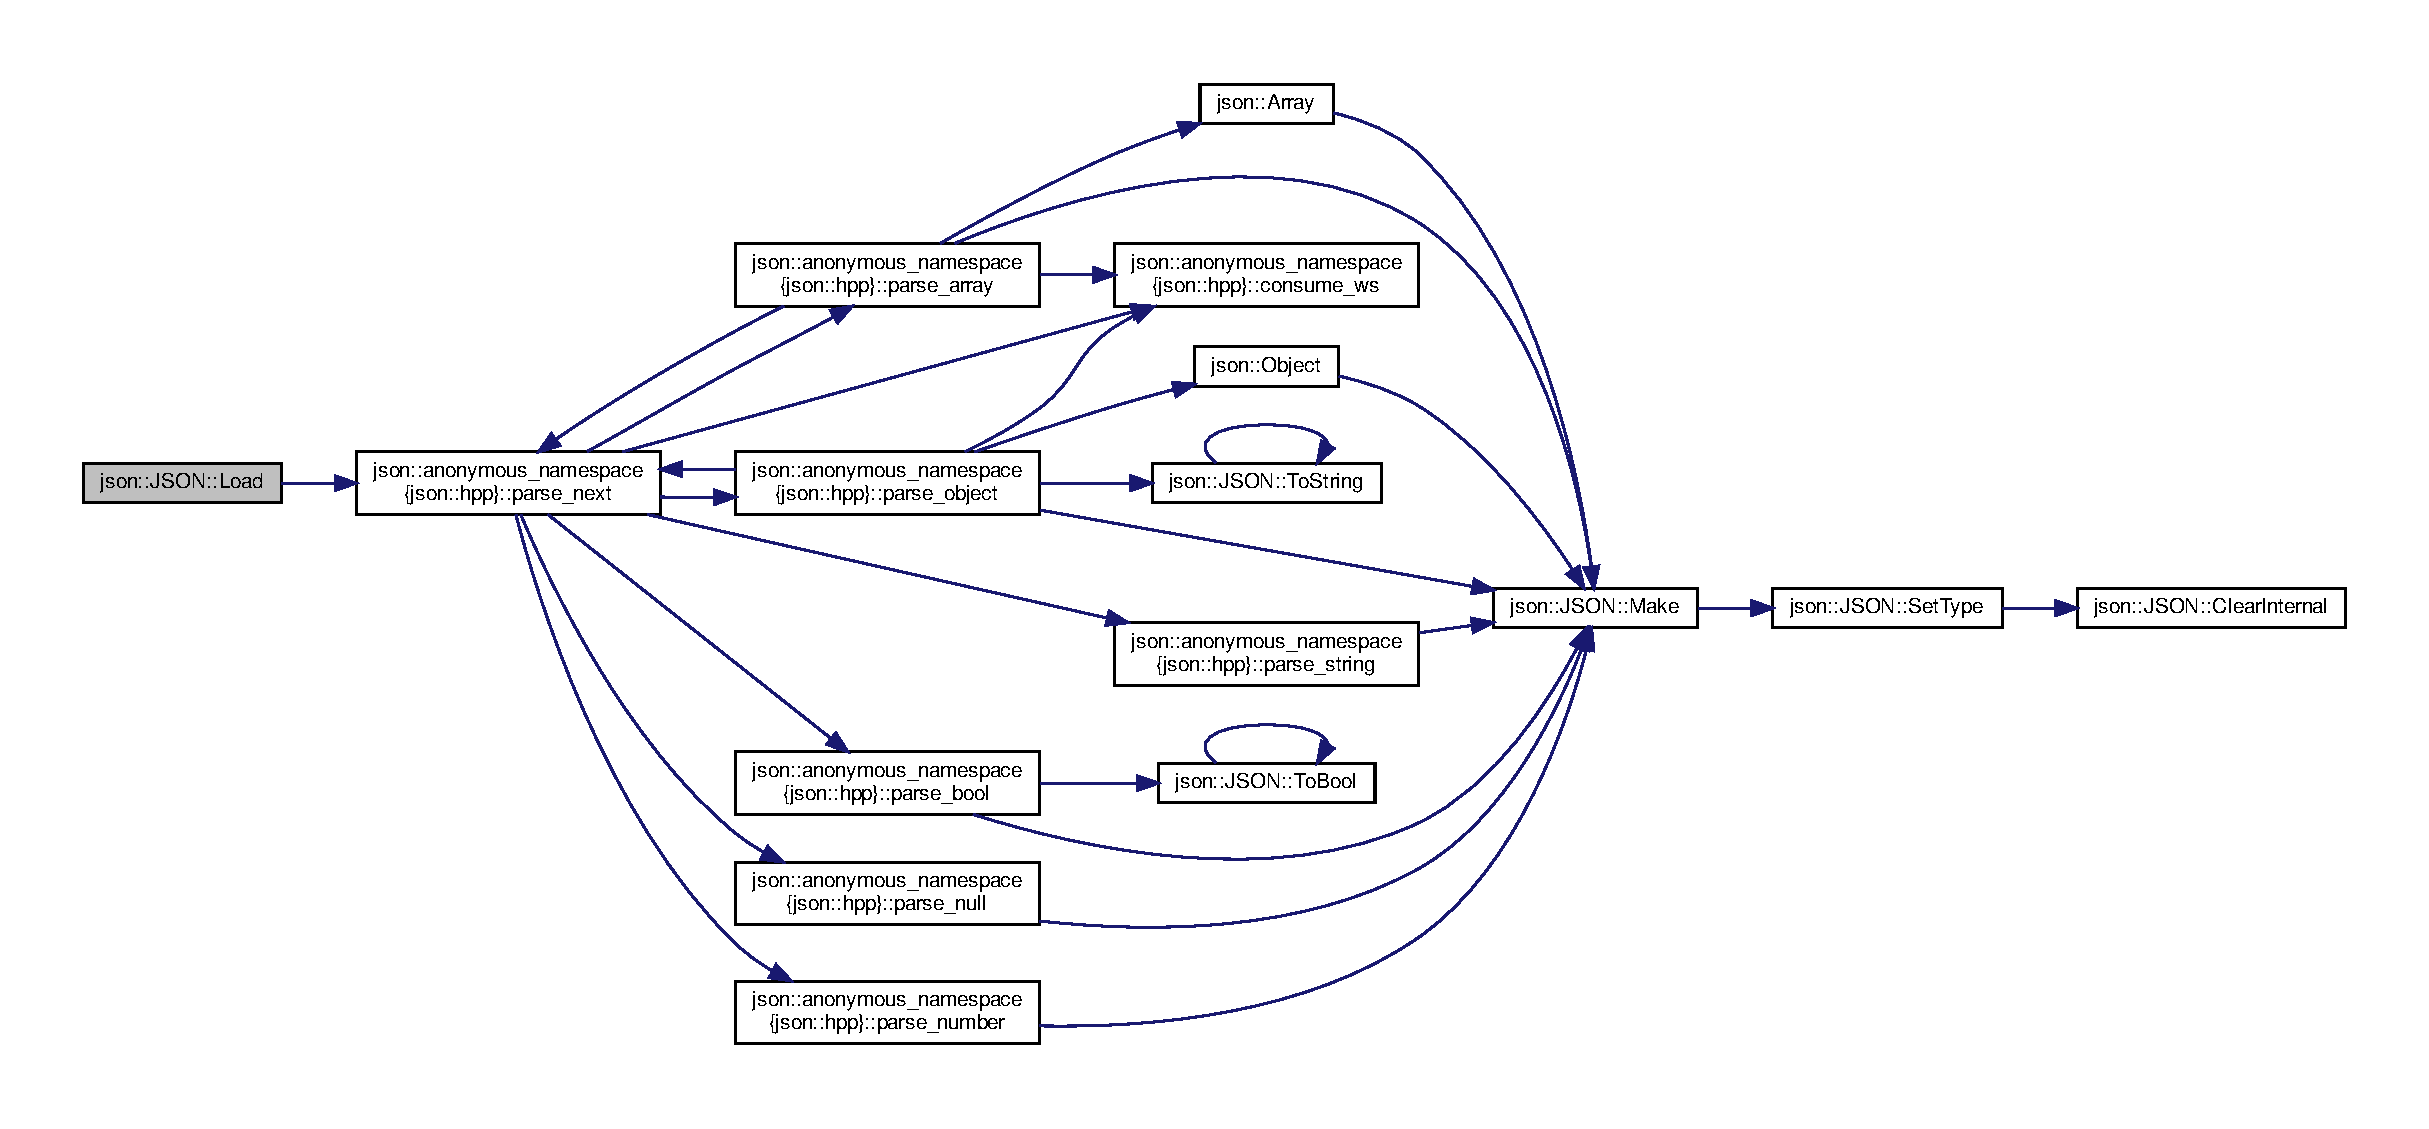
\includegraphics[width=350pt]{classjson_1_1_j_s_o_n_a799ab1cc68cb6e2a41ec948a9a2ecc37_cgraph}
\end{center}
\end{figure}
Here is the caller graph for this function\+:
\nopagebreak
\begin{figure}[H]
\begin{center}
\leavevmode
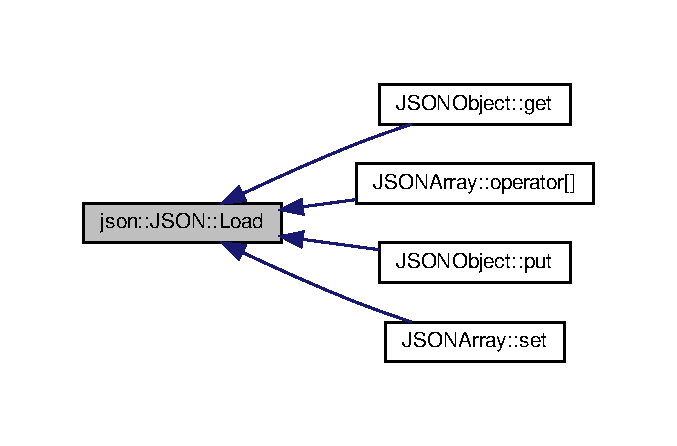
\includegraphics[width=325pt]{classjson_1_1_j_s_o_n_a799ab1cc68cb6e2a41ec948a9a2ecc37_icgraph}
\end{center}
\end{figure}
\mbox{\Hypertarget{classjson_1_1_j_s_o_n_aa679dc348ed9711357c315a461b65957}\label{classjson_1_1_j_s_o_n_aa679dc348ed9711357c315a461b65957}} 
\index{json\+::\+J\+S\+ON@{json\+::\+J\+S\+ON}!Make@{Make}}
\index{Make@{Make}!json\+::\+J\+S\+ON@{json\+::\+J\+S\+ON}}
\subsubsection{\texorpdfstring{Make()}{Make()}}
{\footnotesize\ttfamily static \mbox{\hyperlink{classjson_1_1_j_s_o_n}{J\+S\+ON}} json\+::\+J\+S\+O\+N\+::\+Make (\begin{DoxyParamCaption}\item[{\mbox{\hyperlink{classjson_1_1_j_s_o_n_a762f55df6d407c1af61607ed516ffe07}{Class}}}]{type }\end{DoxyParamCaption})\hspace{0.3cm}{\ttfamily [inline]}, {\ttfamily [static]}}



Definition at line 198 of file json.\+hpp.



References Set\+Type().



Referenced by json\+::\+Array(), json\+::\+Object(), json\+::anonymous\+\_\+namespace\{json.\+hpp\}\+::parse\+\_\+array(), json\+::anonymous\+\_\+namespace\{json.\+hpp\}\+::parse\+\_\+bool(), json\+::anonymous\+\_\+namespace\{json.\+hpp\}\+::parse\+\_\+null(), json\+::anonymous\+\_\+namespace\{json.\+hpp\}\+::parse\+\_\+number(), json\+::anonymous\+\_\+namespace\{json.\+hpp\}\+::parse\+\_\+object(), and json\+::anonymous\+\_\+namespace\{json.\+hpp\}\+::parse\+\_\+string().


\begin{DoxyCode}
198                                        \{
199             \mbox{\hyperlink{class_j_s_o_n}{JSON}} ret; ret.SetType( type );
200             \textcolor{keywordflow}{return} ret;
201         \}
\end{DoxyCode}
Here is the call graph for this function\+:
\nopagebreak
\begin{figure}[H]
\begin{center}
\leavevmode
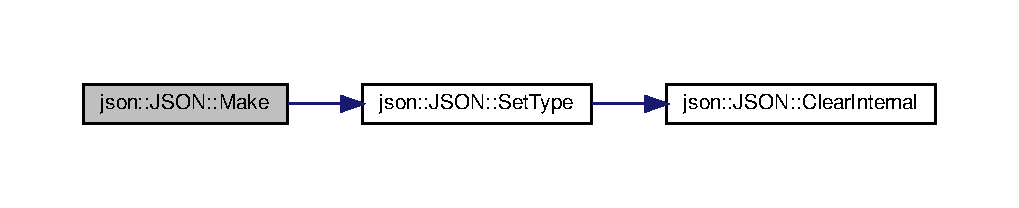
\includegraphics[width=350pt]{classjson_1_1_j_s_o_n_aa679dc348ed9711357c315a461b65957_cgraph}
\end{center}
\end{figure}
Here is the caller graph for this function\+:
\nopagebreak
\begin{figure}[H]
\begin{center}
\leavevmode
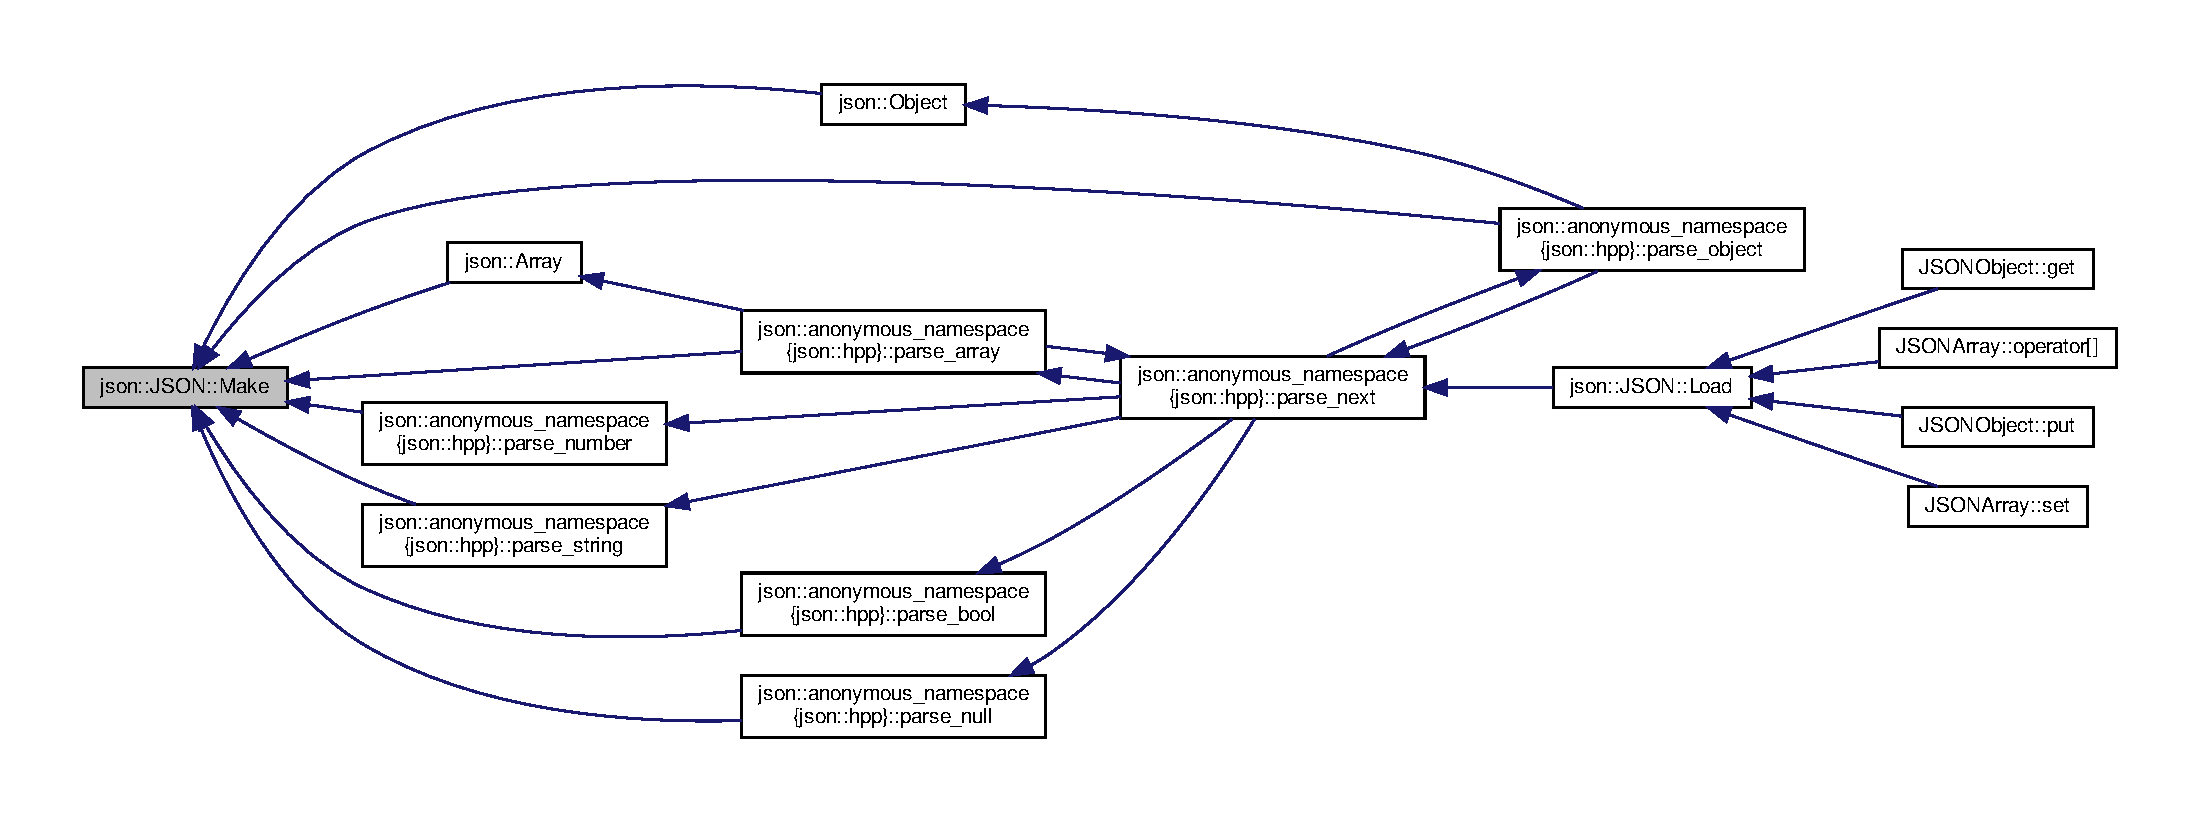
\includegraphics[width=350pt]{classjson_1_1_j_s_o_n_aa679dc348ed9711357c315a461b65957_icgraph}
\end{center}
\end{figure}
\mbox{\Hypertarget{classjson_1_1_j_s_o_n_a5e2527751cd1ae28b29e82fd1de15555}\label{classjson_1_1_j_s_o_n_a5e2527751cd1ae28b29e82fd1de15555}} 
\index{json\+::\+J\+S\+ON@{json\+::\+J\+S\+ON}!Object\+Range@{Object\+Range}}
\index{Object\+Range@{Object\+Range}!json\+::\+J\+S\+ON@{json\+::\+J\+S\+ON}}
\subsubsection{\texorpdfstring{Object\+Range()}{ObjectRange()}\hspace{0.1cm}{\footnotesize\ttfamily [1/2]}}
{\footnotesize\ttfamily \mbox{\hyperlink{classjson_1_1_j_s_o_n_1_1_j_s_o_n_wrapper}{J\+S\+O\+N\+Wrapper}}$<$map$<$string,\mbox{\hyperlink{classjson_1_1_j_s_o_n}{J\+S\+ON}}$>$ $>$ json\+::\+J\+S\+O\+N\+::\+Object\+Range (\begin{DoxyParamCaption}{ }\end{DoxyParamCaption})\hspace{0.3cm}{\ttfamily [inline]}}



Definition at line 312 of file json.\+hpp.



References Internal, json\+::\+J\+S\+O\+N\+::\+Backing\+Data\+::\+Map, Object, and Type.


\begin{DoxyCode}
312                                                     \{
313             \textcolor{keywordflow}{if}( \mbox{\hyperlink{classjson_1_1_j_s_o_n_a3fa6923afa41bdfe38077fbc0079aaf5}{Type}} == \mbox{\hyperlink{classjson_1_1_j_s_o_n_a762f55df6d407c1af61607ed516ffe07a497031794414a552435f90151ac3b54b}{Class::Object}} )
314                 \textcolor{keywordflow}{return} JSONWrapper<map<string,JSON>>( \mbox{\hyperlink{classjson_1_1_j_s_o_n_a1e2a064794c3d55c8bb8887fc5734947}{Internal}}.\mbox{\hyperlink{unionjson_1_1_j_s_o_n_1_1_backing_data_ab2e19b00745b37d2add157ff3a35c431}{Map}} );
315             \textcolor{keywordflow}{return} JSONWrapper<map<string,JSON>>( nullptr );
316         \}
\end{DoxyCode}
\mbox{\Hypertarget{classjson_1_1_j_s_o_n_a23a72db5a52bca8b080334198bb25041}\label{classjson_1_1_j_s_o_n_a23a72db5a52bca8b080334198bb25041}} 
\index{json\+::\+J\+S\+ON@{json\+::\+J\+S\+ON}!Object\+Range@{Object\+Range}}
\index{Object\+Range@{Object\+Range}!json\+::\+J\+S\+ON@{json\+::\+J\+S\+ON}}
\subsubsection{\texorpdfstring{Object\+Range()}{ObjectRange()}\hspace{0.1cm}{\footnotesize\ttfamily [2/2]}}
{\footnotesize\ttfamily \mbox{\hyperlink{classjson_1_1_j_s_o_n_1_1_j_s_o_n_const_wrapper}{J\+S\+O\+N\+Const\+Wrapper}}$<$map$<$string,\mbox{\hyperlink{classjson_1_1_j_s_o_n}{J\+S\+ON}}$>$ $>$ json\+::\+J\+S\+O\+N\+::\+Object\+Range (\begin{DoxyParamCaption}{ }\end{DoxyParamCaption}) const\hspace{0.3cm}{\ttfamily [inline]}}



Definition at line 324 of file json.\+hpp.



References Internal, json\+::\+J\+S\+O\+N\+::\+Backing\+Data\+::\+Map, Object, and Type.


\begin{DoxyCode}
324                                                                \{
325             \textcolor{keywordflow}{if}( \mbox{\hyperlink{classjson_1_1_j_s_o_n_a3fa6923afa41bdfe38077fbc0079aaf5}{Type}} == \mbox{\hyperlink{classjson_1_1_j_s_o_n_a762f55df6d407c1af61607ed516ffe07a497031794414a552435f90151ac3b54b}{Class::Object}} )
326                 \textcolor{keywordflow}{return} JSONConstWrapper<map<string,JSON>>( \mbox{\hyperlink{classjson_1_1_j_s_o_n_a1e2a064794c3d55c8bb8887fc5734947}{Internal}}.\mbox{\hyperlink{unionjson_1_1_j_s_o_n_1_1_backing_data_ab2e19b00745b37d2add157ff3a35c431}{Map}} );
327             \textcolor{keywordflow}{return} JSONConstWrapper<map<string,JSON>>( nullptr );
328         \}
\end{DoxyCode}
\mbox{\Hypertarget{classjson_1_1_j_s_o_n_ab22885428262d4ed0a95c50d5537b13e}\label{classjson_1_1_j_s_o_n_ab22885428262d4ed0a95c50d5537b13e}} 
\index{json\+::\+J\+S\+ON@{json\+::\+J\+S\+ON}!operator=@{operator=}}
\index{operator=@{operator=}!json\+::\+J\+S\+ON@{json\+::\+J\+S\+ON}}
\subsubsection{\texorpdfstring{operator=()}{operator=()}\hspace{0.1cm}{\footnotesize\ttfamily [1/6]}}
{\footnotesize\ttfamily \mbox{\hyperlink{classjson_1_1_j_s_o_n}{J\+S\+ON}}\& json\+::\+J\+S\+O\+N\+::operator= (\begin{DoxyParamCaption}\item[{\mbox{\hyperlink{classjson_1_1_j_s_o_n}{J\+S\+ON}} \&\&}]{other }\end{DoxyParamCaption})\hspace{0.3cm}{\ttfamily [inline]}}



Definition at line 114 of file json.\+hpp.



References Clear\+Internal(), Internal, Null, and Type.


\begin{DoxyCode}
114                                         \{
115             \mbox{\hyperlink{classjson_1_1_j_s_o_n_afefdc8c18c2c40575c2c8463fbd78c67}{ClearInternal}}();
116             \mbox{\hyperlink{classjson_1_1_j_s_o_n_a1e2a064794c3d55c8bb8887fc5734947}{Internal}} = other.Internal;
117             \mbox{\hyperlink{classjson_1_1_j_s_o_n_a3fa6923afa41bdfe38077fbc0079aaf5}{Type}} = other.Type;
118             other.Internal.Map = \textcolor{keyword}{nullptr};
119             other.Type = \mbox{\hyperlink{classjson_1_1_j_s_o_n_a762f55df6d407c1af61607ed516ffe07abbb93ef26e3c101ff11cdd21cab08a94}{Class::Null}};
120             \textcolor{keywordflow}{return} *\textcolor{keyword}{this};
121         \}
\end{DoxyCode}
Here is the call graph for this function\+:
\nopagebreak
\begin{figure}[H]
\begin{center}
\leavevmode
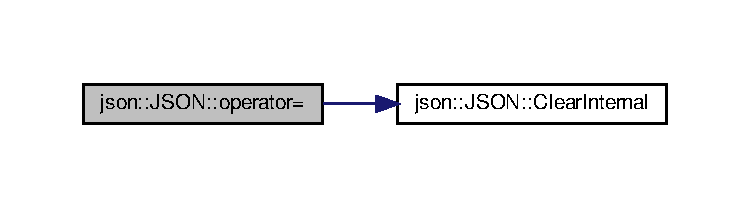
\includegraphics[width=350pt]{classjson_1_1_j_s_o_n_ab22885428262d4ed0a95c50d5537b13e_cgraph}
\end{center}
\end{figure}
\mbox{\Hypertarget{classjson_1_1_j_s_o_n_ac60d87eca03625eb071fb0c98febbb97}\label{classjson_1_1_j_s_o_n_ac60d87eca03625eb071fb0c98febbb97}} 
\index{json\+::\+J\+S\+ON@{json\+::\+J\+S\+ON}!operator=@{operator=}}
\index{operator=@{operator=}!json\+::\+J\+S\+ON@{json\+::\+J\+S\+ON}}
\subsubsection{\texorpdfstring{operator=()}{operator=()}\hspace{0.1cm}{\footnotesize\ttfamily [2/6]}}
{\footnotesize\ttfamily \mbox{\hyperlink{classjson_1_1_j_s_o_n}{J\+S\+ON}}\& json\+::\+J\+S\+O\+N\+::operator= (\begin{DoxyParamCaption}\item[{const \mbox{\hyperlink{classjson_1_1_j_s_o_n}{J\+S\+ON}} \&}]{other }\end{DoxyParamCaption})\hspace{0.3cm}{\ttfamily [inline]}}



Definition at line 145 of file json.\+hpp.



References Array, Clear\+Internal(), Internal, json\+::\+J\+S\+O\+N\+::\+Backing\+Data\+::\+List, json\+::\+J\+S\+O\+N\+::\+Backing\+Data\+::\+Map, Object, json\+::\+J\+S\+O\+N\+::\+Backing\+Data\+::\+String, String, and Type.


\begin{DoxyCode}
145                                              \{
146             \mbox{\hyperlink{classjson_1_1_j_s_o_n_afefdc8c18c2c40575c2c8463fbd78c67}{ClearInternal}}();
147             \textcolor{keywordflow}{switch}( other.Type ) \{
148             \textcolor{keywordflow}{case} \mbox{\hyperlink{classjson_1_1_j_s_o_n_a762f55df6d407c1af61607ed516ffe07a497031794414a552435f90151ac3b54b}{Class::Object}}:
149                 \mbox{\hyperlink{classjson_1_1_j_s_o_n_a1e2a064794c3d55c8bb8887fc5734947}{Internal}}.\mbox{\hyperlink{unionjson_1_1_j_s_o_n_1_1_backing_data_ab2e19b00745b37d2add157ff3a35c431}{Map}} = 
150                     \textcolor{keyword}{new} map<string,JSON>( other.Internal.Map->begin(),
151                                           other.Internal.Map->end() );
152                 \textcolor{keywordflow}{break};
153             \textcolor{keywordflow}{case} \mbox{\hyperlink{classjson_1_1_j_s_o_n_a762f55df6d407c1af61607ed516ffe07a4410ec34d9e6c1a68100ca0ce033fb17}{Class::Array}}:
154                 \mbox{\hyperlink{classjson_1_1_j_s_o_n_a1e2a064794c3d55c8bb8887fc5734947}{Internal}}.\mbox{\hyperlink{unionjson_1_1_j_s_o_n_1_1_backing_data_ab85f5e7ad21f9f7a5407ab73128a3ebc}{List}} = 
155                     \textcolor{keyword}{new} deque<JSON>( other.Internal.List->begin(),
156                                       other.Internal.List->end() );
157                 \textcolor{keywordflow}{break};
158             \textcolor{keywordflow}{case} \mbox{\hyperlink{classjson_1_1_j_s_o_n_a762f55df6d407c1af61607ed516ffe07a27118326006d3829667a400ad23d5d98}{Class::String}}:
159                 \mbox{\hyperlink{classjson_1_1_j_s_o_n_a1e2a064794c3d55c8bb8887fc5734947}{Internal}}.\mbox{\hyperlink{unionjson_1_1_j_s_o_n_1_1_backing_data_a883c18d113d2e55767a9530f06a9c772}{String}} = 
160                     \textcolor{keyword}{new} string( *other.Internal.String );
161                 \textcolor{keywordflow}{break};
162             \textcolor{keywordflow}{default}:
163                 \mbox{\hyperlink{classjson_1_1_j_s_o_n_a1e2a064794c3d55c8bb8887fc5734947}{Internal}} = other.Internal;
164             \}
165             \mbox{\hyperlink{classjson_1_1_j_s_o_n_a3fa6923afa41bdfe38077fbc0079aaf5}{Type}} = other.Type;
166             \textcolor{keywordflow}{return} *\textcolor{keyword}{this};
167         \}
\end{DoxyCode}
Here is the call graph for this function\+:
\nopagebreak
\begin{figure}[H]
\begin{center}
\leavevmode
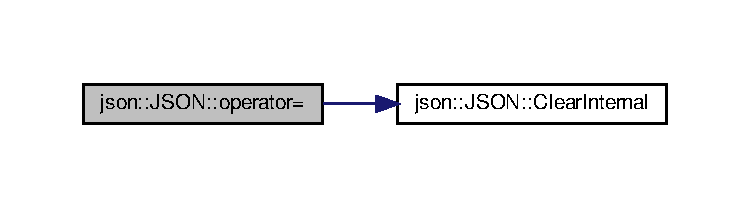
\includegraphics[width=350pt]{classjson_1_1_j_s_o_n_ac60d87eca03625eb071fb0c98febbb97_cgraph}
\end{center}
\end{figure}
\mbox{\Hypertarget{classjson_1_1_j_s_o_n_a1ee7a8f339bd04d78a4db4aa09cc4e53}\label{classjson_1_1_j_s_o_n_a1ee7a8f339bd04d78a4db4aa09cc4e53}} 
\index{json\+::\+J\+S\+ON@{json\+::\+J\+S\+ON}!operator=@{operator=}}
\index{operator=@{operator=}!json\+::\+J\+S\+ON@{json\+::\+J\+S\+ON}}
\subsubsection{\texorpdfstring{operator=()}{operator=()}\hspace{0.1cm}{\footnotesize\ttfamily [3/6]}}
{\footnotesize\ttfamily template$<$typename T $>$ \\
enable\+\_\+if$<$is\+\_\+same$<$T,bool$>$\+::value, \mbox{\hyperlink{classjson_1_1_j_s_o_n}{J\+S\+ON}}\&$>$\+::type json\+::\+J\+S\+O\+N\+::operator= (\begin{DoxyParamCaption}\item[{T}]{b }\end{DoxyParamCaption})\hspace{0.3cm}{\ttfamily [inline]}}



Definition at line 216 of file json.\+hpp.



References json\+::\+J\+S\+O\+N\+::\+Backing\+Data\+::\+Bool, Boolean, Internal, and Set\+Type().


\begin{DoxyCode}
216                                                                                  \{
217                 \mbox{\hyperlink{classjson_1_1_j_s_o_n_a668500208950e48394fc8bfe7c320205}{SetType}}( \mbox{\hyperlink{classjson_1_1_j_s_o_n_a762f55df6d407c1af61607ed516ffe07a27226c864bac7454a8504f8edb15d95b}{Class::Boolean}} ); \mbox{\hyperlink{classjson_1_1_j_s_o_n_a1e2a064794c3d55c8bb8887fc5734947}{Internal}}.
      \mbox{\hyperlink{unionjson_1_1_j_s_o_n_1_1_backing_data_a0659fafaedb7de535ae3e79e4ff4688c}{Bool}} = b; \textcolor{keywordflow}{return} *\textcolor{keyword}{this};
218             \}
\end{DoxyCode}
Here is the call graph for this function\+:
\nopagebreak
\begin{figure}[H]
\begin{center}
\leavevmode
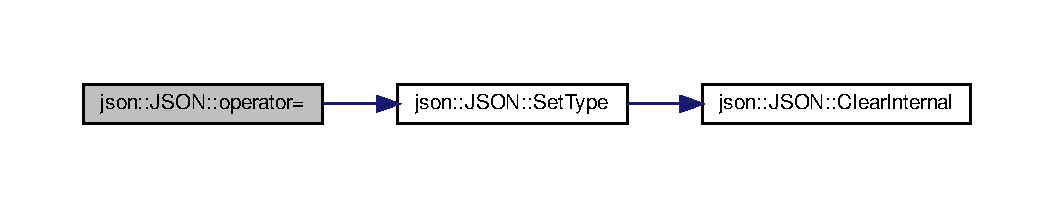
\includegraphics[width=350pt]{classjson_1_1_j_s_o_n_a1ee7a8f339bd04d78a4db4aa09cc4e53_cgraph}
\end{center}
\end{figure}
\mbox{\Hypertarget{classjson_1_1_j_s_o_n_aed9846560a9b7c25b26f684e8d9f32f6}\label{classjson_1_1_j_s_o_n_aed9846560a9b7c25b26f684e8d9f32f6}} 
\index{json\+::\+J\+S\+ON@{json\+::\+J\+S\+ON}!operator=@{operator=}}
\index{operator=@{operator=}!json\+::\+J\+S\+ON@{json\+::\+J\+S\+ON}}
\subsubsection{\texorpdfstring{operator=()}{operator=()}\hspace{0.1cm}{\footnotesize\ttfamily [4/6]}}
{\footnotesize\ttfamily template$<$typename T $>$ \\
enable\+\_\+if$<$is\+\_\+integral$<$T$>$\+::value \&\& !is\+\_\+same$<$T,bool$>$\+::value, \mbox{\hyperlink{classjson_1_1_j_s_o_n}{J\+S\+ON}}\&$>$\+::type json\+::\+J\+S\+O\+N\+::operator= (\begin{DoxyParamCaption}\item[{T}]{i }\end{DoxyParamCaption})\hspace{0.3cm}{\ttfamily [inline]}}



Definition at line 221 of file json.\+hpp.



References json\+::\+J\+S\+O\+N\+::\+Backing\+Data\+::\+Int, Integral, Internal, and Set\+Type().


\begin{DoxyCode}
221                                                                                                          \{
222                 \mbox{\hyperlink{classjson_1_1_j_s_o_n_a668500208950e48394fc8bfe7c320205}{SetType}}( \mbox{\hyperlink{classjson_1_1_j_s_o_n_a762f55df6d407c1af61607ed516ffe07a4ea94552a2bec56a29592359a1b6069e}{Class::Integral}} ); \mbox{\hyperlink{classjson_1_1_j_s_o_n_a1e2a064794c3d55c8bb8887fc5734947}{Internal}}.
      \mbox{\hyperlink{unionjson_1_1_j_s_o_n_1_1_backing_data_a0d80815a70ff5bb9345f75de79ec81c3}{Int}} = i; \textcolor{keywordflow}{return} *\textcolor{keyword}{this};
223             \}
\end{DoxyCode}
Here is the call graph for this function\+:
\nopagebreak
\begin{figure}[H]
\begin{center}
\leavevmode
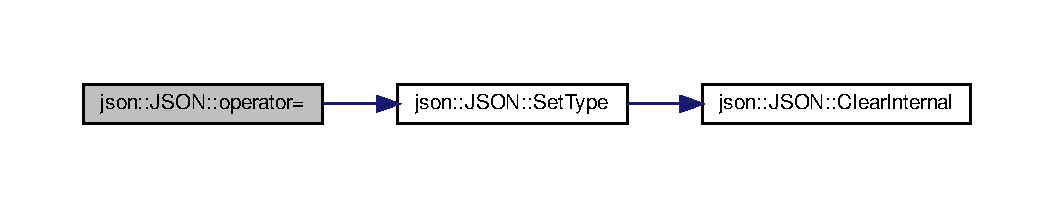
\includegraphics[width=350pt]{classjson_1_1_j_s_o_n_aed9846560a9b7c25b26f684e8d9f32f6_cgraph}
\end{center}
\end{figure}
\mbox{\Hypertarget{classjson_1_1_j_s_o_n_ac272eeeb42a552c4190a320a4f58a062}\label{classjson_1_1_j_s_o_n_ac272eeeb42a552c4190a320a4f58a062}} 
\index{json\+::\+J\+S\+ON@{json\+::\+J\+S\+ON}!operator=@{operator=}}
\index{operator=@{operator=}!json\+::\+J\+S\+ON@{json\+::\+J\+S\+ON}}
\subsubsection{\texorpdfstring{operator=()}{operator=()}\hspace{0.1cm}{\footnotesize\ttfamily [5/6]}}
{\footnotesize\ttfamily template$<$typename T $>$ \\
enable\+\_\+if$<$is\+\_\+floating\+\_\+point$<$T$>$\+::value, \mbox{\hyperlink{classjson_1_1_j_s_o_n}{J\+S\+ON}}\&$>$\+::type json\+::\+J\+S\+O\+N\+::operator= (\begin{DoxyParamCaption}\item[{T}]{f }\end{DoxyParamCaption})\hspace{0.3cm}{\ttfamily [inline]}}



Definition at line 226 of file json.\+hpp.



References json\+::\+J\+S\+O\+N\+::\+Backing\+Data\+::\+Float, Floating, Internal, and Set\+Type().


\begin{DoxyCode}
226                                                                                       \{
227                 \mbox{\hyperlink{classjson_1_1_j_s_o_n_a668500208950e48394fc8bfe7c320205}{SetType}}( \mbox{\hyperlink{classjson_1_1_j_s_o_n_a762f55df6d407c1af61607ed516ffe07ac8df43648942ec3a9aec140f07f47b7c}{Class::Floating}} ); \mbox{\hyperlink{classjson_1_1_j_s_o_n_a1e2a064794c3d55c8bb8887fc5734947}{Internal}}.
      \mbox{\hyperlink{unionjson_1_1_j_s_o_n_1_1_backing_data_aac4950afa6b9205bb367a33de47faa5c}{Float}} = f; \textcolor{keywordflow}{return} *\textcolor{keyword}{this};
228             \}
\end{DoxyCode}
Here is the call graph for this function\+:
\nopagebreak
\begin{figure}[H]
\begin{center}
\leavevmode
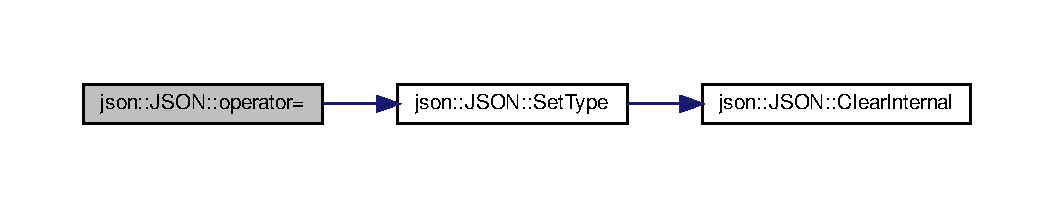
\includegraphics[width=350pt]{classjson_1_1_j_s_o_n_ac272eeeb42a552c4190a320a4f58a062_cgraph}
\end{center}
\end{figure}
\mbox{\Hypertarget{classjson_1_1_j_s_o_n_ab2dd5163c63d60978a2067a2c1ba50ee}\label{classjson_1_1_j_s_o_n_ab2dd5163c63d60978a2067a2c1ba50ee}} 
\index{json\+::\+J\+S\+ON@{json\+::\+J\+S\+ON}!operator=@{operator=}}
\index{operator=@{operator=}!json\+::\+J\+S\+ON@{json\+::\+J\+S\+ON}}
\subsubsection{\texorpdfstring{operator=()}{operator=()}\hspace{0.1cm}{\footnotesize\ttfamily [6/6]}}
{\footnotesize\ttfamily template$<$typename T $>$ \\
enable\+\_\+if$<$is\+\_\+convertible$<$T,string$>$\+::value, \mbox{\hyperlink{classjson_1_1_j_s_o_n}{J\+S\+ON}}\&$>$\+::type json\+::\+J\+S\+O\+N\+::operator= (\begin{DoxyParamCaption}\item[{T}]{s }\end{DoxyParamCaption})\hspace{0.3cm}{\ttfamily [inline]}}



Definition at line 231 of file json.\+hpp.



References Internal, Set\+Type(), json\+::\+J\+S\+O\+N\+::\+Backing\+Data\+::\+String, and String.


\begin{DoxyCode}
231                                                                                           \{
232                 \mbox{\hyperlink{classjson_1_1_j_s_o_n_a668500208950e48394fc8bfe7c320205}{SetType}}( \mbox{\hyperlink{classjson_1_1_j_s_o_n_a762f55df6d407c1af61607ed516ffe07a27118326006d3829667a400ad23d5d98}{Class::String}} ); *\mbox{\hyperlink{classjson_1_1_j_s_o_n_a1e2a064794c3d55c8bb8887fc5734947}{Internal}}.
      \mbox{\hyperlink{unionjson_1_1_j_s_o_n_1_1_backing_data_a883c18d113d2e55767a9530f06a9c772}{String}} = string( s ); \textcolor{keywordflow}{return} *\textcolor{keyword}{this};
233             \}
\end{DoxyCode}
Here is the call graph for this function\+:
\nopagebreak
\begin{figure}[H]
\begin{center}
\leavevmode
\includegraphics[width=350pt]{classjson_1_1_j_s_o_n_ab2dd5163c63d60978a2067a2c1ba50ee_cgraph}
\end{center}
\end{figure}
\mbox{\Hypertarget{classjson_1_1_j_s_o_n_a29c695c67a5b34a3b59af0da3c25d6b1}\label{classjson_1_1_j_s_o_n_a29c695c67a5b34a3b59af0da3c25d6b1}} 
\index{json\+::\+J\+S\+ON@{json\+::\+J\+S\+ON}!operator\mbox{[}\mbox{]}@{operator[]}}
\index{operator\mbox{[}\mbox{]}@{operator[]}!json\+::\+J\+S\+ON@{json\+::\+J\+S\+ON}}
\subsubsection{\texorpdfstring{operator[]()}{operator[]()}\hspace{0.1cm}{\footnotesize\ttfamily [1/2]}}
{\footnotesize\ttfamily \mbox{\hyperlink{classjson_1_1_j_s_o_n}{J\+S\+ON}}\& json\+::\+J\+S\+O\+N\+::operator\mbox{[}$\,$\mbox{]} (\begin{DoxyParamCaption}\item[{const string \&}]{key }\end{DoxyParamCaption})\hspace{0.3cm}{\ttfamily [inline]}}



Definition at line 235 of file json.\+hpp.



References Internal, json\+::\+J\+S\+O\+N\+::\+Backing\+Data\+::\+Map, Object, and Set\+Type().



Referenced by at().


\begin{DoxyCode}
235                                               \{
236             \mbox{\hyperlink{classjson_1_1_j_s_o_n_a668500208950e48394fc8bfe7c320205}{SetType}}( \mbox{\hyperlink{classjson_1_1_j_s_o_n_a762f55df6d407c1af61607ed516ffe07a497031794414a552435f90151ac3b54b}{Class::Object}} ); \textcolor{keywordflow}{return} \mbox{\hyperlink{classjson_1_1_j_s_o_n_a1e2a064794c3d55c8bb8887fc5734947}{Internal}}.
      \mbox{\hyperlink{unionjson_1_1_j_s_o_n_1_1_backing_data_ab2e19b00745b37d2add157ff3a35c431}{Map}}->operator[]( key );
237         \}
\end{DoxyCode}
Here is the call graph for this function\+:
\nopagebreak
\begin{figure}[H]
\begin{center}
\leavevmode
\includegraphics[width=350pt]{classjson_1_1_j_s_o_n_a29c695c67a5b34a3b59af0da3c25d6b1_cgraph}
\end{center}
\end{figure}
Here is the caller graph for this function\+:
\nopagebreak
\begin{figure}[H]
\begin{center}
\leavevmode
\includegraphics[width=313pt]{classjson_1_1_j_s_o_n_a29c695c67a5b34a3b59af0da3c25d6b1_icgraph}
\end{center}
\end{figure}
\mbox{\Hypertarget{classjson_1_1_j_s_o_n_ad590ba3c1aa11aad67e03138ffdc1488}\label{classjson_1_1_j_s_o_n_ad590ba3c1aa11aad67e03138ffdc1488}} 
\index{json\+::\+J\+S\+ON@{json\+::\+J\+S\+ON}!operator\mbox{[}\mbox{]}@{operator[]}}
\index{operator\mbox{[}\mbox{]}@{operator[]}!json\+::\+J\+S\+ON@{json\+::\+J\+S\+ON}}
\subsubsection{\texorpdfstring{operator[]()}{operator[]()}\hspace{0.1cm}{\footnotesize\ttfamily [2/2]}}
{\footnotesize\ttfamily \mbox{\hyperlink{classjson_1_1_j_s_o_n}{J\+S\+ON}}\& json\+::\+J\+S\+O\+N\+::operator\mbox{[}$\,$\mbox{]} (\begin{DoxyParamCaption}\item[{unsigned}]{index }\end{DoxyParamCaption})\hspace{0.3cm}{\ttfamily [inline]}}



Definition at line 239 of file json.\+hpp.



References Array, Internal, json\+::\+J\+S\+O\+N\+::\+Backing\+Data\+::\+List, and Set\+Type().


\begin{DoxyCode}
239                                            \{
240             \mbox{\hyperlink{classjson_1_1_j_s_o_n_a668500208950e48394fc8bfe7c320205}{SetType}}( \mbox{\hyperlink{classjson_1_1_j_s_o_n_a762f55df6d407c1af61607ed516ffe07a4410ec34d9e6c1a68100ca0ce033fb17}{Class::Array}} );
241             \textcolor{keywordflow}{if}( index >= \mbox{\hyperlink{classjson_1_1_j_s_o_n_a1e2a064794c3d55c8bb8887fc5734947}{Internal}}.\mbox{\hyperlink{unionjson_1_1_j_s_o_n_1_1_backing_data_ab85f5e7ad21f9f7a5407ab73128a3ebc}{List}}->size() ) \mbox{\hyperlink{classjson_1_1_j_s_o_n_a1e2a064794c3d55c8bb8887fc5734947}{Internal}}.
      \mbox{\hyperlink{unionjson_1_1_j_s_o_n_1_1_backing_data_ab85f5e7ad21f9f7a5407ab73128a3ebc}{List}}->resize( index + 1 );
242             \textcolor{keywordflow}{return} \mbox{\hyperlink{classjson_1_1_j_s_o_n_a1e2a064794c3d55c8bb8887fc5734947}{Internal}}.\mbox{\hyperlink{unionjson_1_1_j_s_o_n_1_1_backing_data_ab85f5e7ad21f9f7a5407ab73128a3ebc}{List}}->operator[]( index );
243         \}
\end{DoxyCode}
Here is the call graph for this function\+:
\nopagebreak
\begin{figure}[H]
\begin{center}
\leavevmode
\includegraphics[width=350pt]{classjson_1_1_j_s_o_n_ad590ba3c1aa11aad67e03138ffdc1488_cgraph}
\end{center}
\end{figure}
\mbox{\Hypertarget{classjson_1_1_j_s_o_n_a668500208950e48394fc8bfe7c320205}\label{classjson_1_1_j_s_o_n_a668500208950e48394fc8bfe7c320205}} 
\index{json\+::\+J\+S\+ON@{json\+::\+J\+S\+ON}!Set\+Type@{Set\+Type}}
\index{Set\+Type@{Set\+Type}!json\+::\+J\+S\+ON@{json\+::\+J\+S\+ON}}
\subsubsection{\texorpdfstring{Set\+Type()}{SetType()}}
{\footnotesize\ttfamily void json\+::\+J\+S\+O\+N\+::\+Set\+Type (\begin{DoxyParamCaption}\item[{\mbox{\hyperlink{classjson_1_1_j_s_o_n_a762f55df6d407c1af61607ed516ffe07}{Class}}}]{type }\end{DoxyParamCaption})\hspace{0.3cm}{\ttfamily [inline]}, {\ttfamily [private]}}



Definition at line 383 of file json.\+hpp.



References Array, json\+::\+J\+S\+O\+N\+::\+Backing\+Data\+::\+Bool, Boolean, Clear\+Internal(), json\+::\+J\+S\+O\+N\+::\+Backing\+Data\+::\+Float, Floating, json\+::\+J\+S\+O\+N\+::\+Backing\+Data\+::\+Int, Integral, Internal, json\+::\+J\+S\+O\+N\+::\+Backing\+Data\+::\+List, json\+::\+J\+S\+O\+N\+::\+Backing\+Data\+::\+Map, Null, Object, json\+::\+J\+S\+O\+N\+::\+Backing\+Data\+::\+String, String, and Type.



Referenced by append(), J\+S\+O\+N(), Make(), operator=(), and operator\mbox{[}$\,$\mbox{]}().


\begin{DoxyCode}
383                                    \{
384             \textcolor{keywordflow}{if}( type == \mbox{\hyperlink{classjson_1_1_j_s_o_n_a3fa6923afa41bdfe38077fbc0079aaf5}{Type}} )
385                 \textcolor{keywordflow}{return};
386 
387             \mbox{\hyperlink{classjson_1_1_j_s_o_n_afefdc8c18c2c40575c2c8463fbd78c67}{ClearInternal}}();
388           
389             \textcolor{keywordflow}{switch}( type ) \{
390             \textcolor{keywordflow}{case} \mbox{\hyperlink{classjson_1_1_j_s_o_n_a762f55df6d407c1af61607ed516ffe07abbb93ef26e3c101ff11cdd21cab08a94}{Class::Null}}:      \mbox{\hyperlink{classjson_1_1_j_s_o_n_a1e2a064794c3d55c8bb8887fc5734947}{Internal}}.\mbox{\hyperlink{unionjson_1_1_j_s_o_n_1_1_backing_data_ab2e19b00745b37d2add157ff3a35c431}{Map}}    = \textcolor{keyword}{nullptr};                \textcolor{keywordflow}{break};
391             \textcolor{keywordflow}{case} \mbox{\hyperlink{classjson_1_1_j_s_o_n_a762f55df6d407c1af61607ed516ffe07a497031794414a552435f90151ac3b54b}{Class::Object}}:    \mbox{\hyperlink{classjson_1_1_j_s_o_n_a1e2a064794c3d55c8bb8887fc5734947}{Internal}}.\mbox{\hyperlink{unionjson_1_1_j_s_o_n_1_1_backing_data_ab2e19b00745b37d2add157ff3a35c431}{Map}}    = \textcolor{keyword}{new} map<string,JSON>(); \textcolor{keywordflow}{break};
392             \textcolor{keywordflow}{case} \mbox{\hyperlink{classjson_1_1_j_s_o_n_a762f55df6d407c1af61607ed516ffe07a4410ec34d9e6c1a68100ca0ce033fb17}{Class::Array}}:     \mbox{\hyperlink{classjson_1_1_j_s_o_n_a1e2a064794c3d55c8bb8887fc5734947}{Internal}}.\mbox{\hyperlink{unionjson_1_1_j_s_o_n_1_1_backing_data_ab85f5e7ad21f9f7a5407ab73128a3ebc}{List}}   = \textcolor{keyword}{new} deque<JSON>();     \textcolor{keywordflow}{break};
393             \textcolor{keywordflow}{case} \mbox{\hyperlink{classjson_1_1_j_s_o_n_a762f55df6d407c1af61607ed516ffe07a27118326006d3829667a400ad23d5d98}{Class::String}}:    \mbox{\hyperlink{classjson_1_1_j_s_o_n_a1e2a064794c3d55c8bb8887fc5734947}{Internal}}.\mbox{\hyperlink{unionjson_1_1_j_s_o_n_1_1_backing_data_a883c18d113d2e55767a9530f06a9c772}{String}} = \textcolor{keyword}{new} string();           \textcolor{keywordflow}{
      break};
394             \textcolor{keywordflow}{case} \mbox{\hyperlink{classjson_1_1_j_s_o_n_a762f55df6d407c1af61607ed516ffe07ac8df43648942ec3a9aec140f07f47b7c}{Class::Floating}}:  \mbox{\hyperlink{classjson_1_1_j_s_o_n_a1e2a064794c3d55c8bb8887fc5734947}{Internal}}.\mbox{\hyperlink{unionjson_1_1_j_s_o_n_1_1_backing_data_aac4950afa6b9205bb367a33de47faa5c}{Float}}  = 0.0;                    \textcolor{keywordflow}{
      break};
395             \textcolor{keywordflow}{case} \mbox{\hyperlink{classjson_1_1_j_s_o_n_a762f55df6d407c1af61607ed516ffe07a4ea94552a2bec56a29592359a1b6069e}{Class::Integral}}:  \mbox{\hyperlink{classjson_1_1_j_s_o_n_a1e2a064794c3d55c8bb8887fc5734947}{Internal}}.\mbox{\hyperlink{unionjson_1_1_j_s_o_n_1_1_backing_data_a0d80815a70ff5bb9345f75de79ec81c3}{Int}}    = 0;                      \textcolor{keywordflow}{
      break};
396             \textcolor{keywordflow}{case} \mbox{\hyperlink{classjson_1_1_j_s_o_n_a762f55df6d407c1af61607ed516ffe07a27226c864bac7454a8504f8edb15d95b}{Class::Boolean}}:   \mbox{\hyperlink{classjson_1_1_j_s_o_n_a1e2a064794c3d55c8bb8887fc5734947}{Internal}}.\mbox{\hyperlink{unionjson_1_1_j_s_o_n_1_1_backing_data_a0659fafaedb7de535ae3e79e4ff4688c}{Bool}}   = \textcolor{keyword}{false};                  \textcolor{keywordflow}{
      break};
397             \}
398 
399             \mbox{\hyperlink{classjson_1_1_j_s_o_n_a3fa6923afa41bdfe38077fbc0079aaf5}{Type}} = type;
400         \}
\end{DoxyCode}
Here is the call graph for this function\+:
\nopagebreak
\begin{figure}[H]
\begin{center}
\leavevmode
\includegraphics[width=350pt]{classjson_1_1_j_s_o_n_a668500208950e48394fc8bfe7c320205_cgraph}
\end{center}
\end{figure}
Here is the caller graph for this function\+:
\nopagebreak
\begin{figure}[H]
\begin{center}
\leavevmode
\includegraphics[width=350pt]{classjson_1_1_j_s_o_n_a668500208950e48394fc8bfe7c320205_icgraph}
\end{center}
\end{figure}
\mbox{\Hypertarget{classjson_1_1_j_s_o_n_af8665d4f94afa84c3e20d52a7184f7ee}\label{classjson_1_1_j_s_o_n_af8665d4f94afa84c3e20d52a7184f7ee}} 
\index{json\+::\+J\+S\+ON@{json\+::\+J\+S\+ON}!size@{size}}
\index{size@{size}!json\+::\+J\+S\+ON@{json\+::\+J\+S\+ON}}
\subsubsection{\texorpdfstring{size()}{size()}}
{\footnotesize\ttfamily int json\+::\+J\+S\+O\+N\+::size (\begin{DoxyParamCaption}{ }\end{DoxyParamCaption}) const\hspace{0.3cm}{\ttfamily [inline]}}



Definition at line 274 of file json.\+hpp.



References Array, Internal, json\+::\+J\+S\+O\+N\+::\+Backing\+Data\+::\+List, json\+::\+J\+S\+O\+N\+::\+Backing\+Data\+::\+Map, Object, and Type.


\begin{DoxyCode}
274                          \{
275             \textcolor{keywordflow}{if}( \mbox{\hyperlink{classjson_1_1_j_s_o_n_a3fa6923afa41bdfe38077fbc0079aaf5}{Type}} == \mbox{\hyperlink{classjson_1_1_j_s_o_n_a762f55df6d407c1af61607ed516ffe07a497031794414a552435f90151ac3b54b}{Class::Object}} )
276                 \textcolor{keywordflow}{return} \mbox{\hyperlink{classjson_1_1_j_s_o_n_a1e2a064794c3d55c8bb8887fc5734947}{Internal}}.\mbox{\hyperlink{unionjson_1_1_j_s_o_n_1_1_backing_data_ab2e19b00745b37d2add157ff3a35c431}{Map}}->size();
277             \textcolor{keywordflow}{else} \textcolor{keywordflow}{if}( \mbox{\hyperlink{classjson_1_1_j_s_o_n_a3fa6923afa41bdfe38077fbc0079aaf5}{Type}} == \mbox{\hyperlink{classjson_1_1_j_s_o_n_a762f55df6d407c1af61607ed516ffe07a4410ec34d9e6c1a68100ca0ce033fb17}{Class::Array}} )
278                 \textcolor{keywordflow}{return} \mbox{\hyperlink{classjson_1_1_j_s_o_n_a1e2a064794c3d55c8bb8887fc5734947}{Internal}}.\mbox{\hyperlink{unionjson_1_1_j_s_o_n_1_1_backing_data_ab85f5e7ad21f9f7a5407ab73128a3ebc}{List}}->size();
279             \textcolor{keywordflow}{else}
280                 \textcolor{keywordflow}{return} -1;
281         \}
\end{DoxyCode}
\mbox{\Hypertarget{classjson_1_1_j_s_o_n_adb9ab4683ee30055912b47220780de16}\label{classjson_1_1_j_s_o_n_adb9ab4683ee30055912b47220780de16}} 
\index{json\+::\+J\+S\+ON@{json\+::\+J\+S\+ON}!To\+Bool@{To\+Bool}}
\index{To\+Bool@{To\+Bool}!json\+::\+J\+S\+ON@{json\+::\+J\+S\+ON}}
\subsubsection{\texorpdfstring{To\+Bool()}{ToBool()}\hspace{0.1cm}{\footnotesize\ttfamily [1/2]}}
{\footnotesize\ttfamily bool json\+::\+J\+S\+O\+N\+::\+To\+Bool (\begin{DoxyParamCaption}{ }\end{DoxyParamCaption}) const\hspace{0.3cm}{\ttfamily [inline]}}



Definition at line 306 of file json.\+hpp.



References To\+Bool().



Referenced by json\+::anonymous\+\_\+namespace\{json.\+hpp\}\+::parse\+\_\+bool(), and To\+Bool().


\begin{DoxyCode}
306 \{ \textcolor{keywordtype}{bool} b; \textcolor{keywordflow}{return} \mbox{\hyperlink{classjson_1_1_j_s_o_n_adb9ab4683ee30055912b47220780de16}{ToBool}}( b ); \}
\end{DoxyCode}
Here is the call graph for this function\+:
\nopagebreak
\begin{figure}[H]
\begin{center}
\leavevmode
\includegraphics[width=184pt]{classjson_1_1_j_s_o_n_adb9ab4683ee30055912b47220780de16_cgraph}
\end{center}
\end{figure}
Here is the caller graph for this function\+:
\nopagebreak
\begin{figure}[H]
\begin{center}
\leavevmode
\includegraphics[width=350pt]{classjson_1_1_j_s_o_n_adb9ab4683ee30055912b47220780de16_icgraph}
\end{center}
\end{figure}
\mbox{\Hypertarget{classjson_1_1_j_s_o_n_aa86f03b8572b13dd768c902da2d83efa}\label{classjson_1_1_j_s_o_n_aa86f03b8572b13dd768c902da2d83efa}} 
\index{json\+::\+J\+S\+ON@{json\+::\+J\+S\+ON}!To\+Bool@{To\+Bool}}
\index{To\+Bool@{To\+Bool}!json\+::\+J\+S\+ON@{json\+::\+J\+S\+ON}}
\subsubsection{\texorpdfstring{To\+Bool()}{ToBool()}\hspace{0.1cm}{\footnotesize\ttfamily [2/2]}}
{\footnotesize\ttfamily bool json\+::\+J\+S\+O\+N\+::\+To\+Bool (\begin{DoxyParamCaption}\item[{bool \&}]{ok }\end{DoxyParamCaption}) const\hspace{0.3cm}{\ttfamily [inline]}}



Definition at line 307 of file json.\+hpp.



References json\+::\+J\+S\+O\+N\+::\+Backing\+Data\+::\+Bool, Boolean, Internal, and Type.


\begin{DoxyCode}
307                                       \{
308             ok = (\mbox{\hyperlink{classjson_1_1_j_s_o_n_a3fa6923afa41bdfe38077fbc0079aaf5}{Type}} == \mbox{\hyperlink{classjson_1_1_j_s_o_n_a762f55df6d407c1af61607ed516ffe07a27226c864bac7454a8504f8edb15d95b}{Class::Boolean}});
309             \textcolor{keywordflow}{return} ok ? \mbox{\hyperlink{classjson_1_1_j_s_o_n_a1e2a064794c3d55c8bb8887fc5734947}{Internal}}.\mbox{\hyperlink{unionjson_1_1_j_s_o_n_1_1_backing_data_a0659fafaedb7de535ae3e79e4ff4688c}{Bool}} : \textcolor{keyword}{false};
310         \}
\end{DoxyCode}
\mbox{\Hypertarget{classjson_1_1_j_s_o_n_ae6ff6af2be133af569a9c3dd38f67d93}\label{classjson_1_1_j_s_o_n_ae6ff6af2be133af569a9c3dd38f67d93}} 
\index{json\+::\+J\+S\+ON@{json\+::\+J\+S\+ON}!To\+Float@{To\+Float}}
\index{To\+Float@{To\+Float}!json\+::\+J\+S\+ON@{json\+::\+J\+S\+ON}}
\subsubsection{\texorpdfstring{To\+Float()}{ToFloat()}\hspace{0.1cm}{\footnotesize\ttfamily [1/2]}}
{\footnotesize\ttfamily double json\+::\+J\+S\+O\+N\+::\+To\+Float (\begin{DoxyParamCaption}{ }\end{DoxyParamCaption}) const\hspace{0.3cm}{\ttfamily [inline]}}



Definition at line 294 of file json.\+hpp.



References To\+Float().



Referenced by To\+Float().


\begin{DoxyCode}
294 \{ \textcolor{keywordtype}{bool} b; \textcolor{keywordflow}{return} \mbox{\hyperlink{classjson_1_1_j_s_o_n_ae6ff6af2be133af569a9c3dd38f67d93}{ToFloat}}( b ); \}
\end{DoxyCode}
Here is the call graph for this function\+:
\nopagebreak
\begin{figure}[H]
\begin{center}
\leavevmode
\includegraphics[width=186pt]{classjson_1_1_j_s_o_n_ae6ff6af2be133af569a9c3dd38f67d93_cgraph}
\end{center}
\end{figure}
Here is the caller graph for this function\+:
\nopagebreak
\begin{figure}[H]
\begin{center}
\leavevmode
\includegraphics[width=186pt]{classjson_1_1_j_s_o_n_ae6ff6af2be133af569a9c3dd38f67d93_icgraph}
\end{center}
\end{figure}
\mbox{\Hypertarget{classjson_1_1_j_s_o_n_ae913234cd95a1338faf8e198b5a0eb38}\label{classjson_1_1_j_s_o_n_ae913234cd95a1338faf8e198b5a0eb38}} 
\index{json\+::\+J\+S\+ON@{json\+::\+J\+S\+ON}!To\+Float@{To\+Float}}
\index{To\+Float@{To\+Float}!json\+::\+J\+S\+ON@{json\+::\+J\+S\+ON}}
\subsubsection{\texorpdfstring{To\+Float()}{ToFloat()}\hspace{0.1cm}{\footnotesize\ttfamily [2/2]}}
{\footnotesize\ttfamily double json\+::\+J\+S\+O\+N\+::\+To\+Float (\begin{DoxyParamCaption}\item[{bool \&}]{ok }\end{DoxyParamCaption}) const\hspace{0.3cm}{\ttfamily [inline]}}



Definition at line 295 of file json.\+hpp.



References json\+::\+J\+S\+O\+N\+::\+Backing\+Data\+::\+Float, Floating, Internal, and Type.


\begin{DoxyCode}
295                                          \{
296             ok = (\mbox{\hyperlink{classjson_1_1_j_s_o_n_a3fa6923afa41bdfe38077fbc0079aaf5}{Type}} == \mbox{\hyperlink{classjson_1_1_j_s_o_n_a762f55df6d407c1af61607ed516ffe07ac8df43648942ec3a9aec140f07f47b7c}{Class::Floating}});
297             \textcolor{keywordflow}{return} ok ? \mbox{\hyperlink{classjson_1_1_j_s_o_n_a1e2a064794c3d55c8bb8887fc5734947}{Internal}}.\mbox{\hyperlink{unionjson_1_1_j_s_o_n_1_1_backing_data_aac4950afa6b9205bb367a33de47faa5c}{Float}} : 0.0;
298         \}
\end{DoxyCode}
\mbox{\Hypertarget{classjson_1_1_j_s_o_n_a867eb9869140b69428287c98d4f56388}\label{classjson_1_1_j_s_o_n_a867eb9869140b69428287c98d4f56388}} 
\index{json\+::\+J\+S\+ON@{json\+::\+J\+S\+ON}!To\+Int@{To\+Int}}
\index{To\+Int@{To\+Int}!json\+::\+J\+S\+ON@{json\+::\+J\+S\+ON}}
\subsubsection{\texorpdfstring{To\+Int()}{ToInt()}\hspace{0.1cm}{\footnotesize\ttfamily [1/2]}}
{\footnotesize\ttfamily long json\+::\+J\+S\+O\+N\+::\+To\+Int (\begin{DoxyParamCaption}{ }\end{DoxyParamCaption}) const\hspace{0.3cm}{\ttfamily [inline]}}



Definition at line 300 of file json.\+hpp.



References To\+Int().



Referenced by To\+Int().


\begin{DoxyCode}
300 \{ \textcolor{keywordtype}{bool} b; \textcolor{keywordflow}{return} \mbox{\hyperlink{classjson_1_1_j_s_o_n_a867eb9869140b69428287c98d4f56388}{ToInt}}( b ); \}
\end{DoxyCode}
Here is the call graph for this function\+:
\nopagebreak
\begin{figure}[H]
\begin{center}
\leavevmode
\includegraphics[width=175pt]{classjson_1_1_j_s_o_n_a867eb9869140b69428287c98d4f56388_cgraph}
\end{center}
\end{figure}
Here is the caller graph for this function\+:
\nopagebreak
\begin{figure}[H]
\begin{center}
\leavevmode
\includegraphics[width=175pt]{classjson_1_1_j_s_o_n_a867eb9869140b69428287c98d4f56388_icgraph}
\end{center}
\end{figure}
\mbox{\Hypertarget{classjson_1_1_j_s_o_n_a12e5b118ced359fd4a315c95a7486007}\label{classjson_1_1_j_s_o_n_a12e5b118ced359fd4a315c95a7486007}} 
\index{json\+::\+J\+S\+ON@{json\+::\+J\+S\+ON}!To\+Int@{To\+Int}}
\index{To\+Int@{To\+Int}!json\+::\+J\+S\+ON@{json\+::\+J\+S\+ON}}
\subsubsection{\texorpdfstring{To\+Int()}{ToInt()}\hspace{0.1cm}{\footnotesize\ttfamily [2/2]}}
{\footnotesize\ttfamily long json\+::\+J\+S\+O\+N\+::\+To\+Int (\begin{DoxyParamCaption}\item[{bool \&}]{ok }\end{DoxyParamCaption}) const\hspace{0.3cm}{\ttfamily [inline]}}



Definition at line 301 of file json.\+hpp.



References json\+::\+J\+S\+O\+N\+::\+Backing\+Data\+::\+Int, Integral, Internal, and Type.


\begin{DoxyCode}
301                                      \{
302             ok = (\mbox{\hyperlink{classjson_1_1_j_s_o_n_a3fa6923afa41bdfe38077fbc0079aaf5}{Type}} == \mbox{\hyperlink{classjson_1_1_j_s_o_n_a762f55df6d407c1af61607ed516ffe07a4ea94552a2bec56a29592359a1b6069e}{Class::Integral}});
303             \textcolor{keywordflow}{return} ok ? \mbox{\hyperlink{classjson_1_1_j_s_o_n_a1e2a064794c3d55c8bb8887fc5734947}{Internal}}.\mbox{\hyperlink{unionjson_1_1_j_s_o_n_1_1_backing_data_a0d80815a70ff5bb9345f75de79ec81c3}{Int}} : 0;
304         \}
\end{DoxyCode}
\mbox{\Hypertarget{classjson_1_1_j_s_o_n_a5f1c7695d59c4652f01cb087eff954f5}\label{classjson_1_1_j_s_o_n_a5f1c7695d59c4652f01cb087eff954f5}} 
\index{json\+::\+J\+S\+ON@{json\+::\+J\+S\+ON}!To\+String@{To\+String}}
\index{To\+String@{To\+String}!json\+::\+J\+S\+ON@{json\+::\+J\+S\+ON}}
\subsubsection{\texorpdfstring{To\+String()}{ToString()}\hspace{0.1cm}{\footnotesize\ttfamily [1/2]}}
{\footnotesize\ttfamily string json\+::\+J\+S\+O\+N\+::\+To\+String (\begin{DoxyParamCaption}{ }\end{DoxyParamCaption}) const\hspace{0.3cm}{\ttfamily [inline]}}



Definition at line 288 of file json.\+hpp.



References To\+String().



Referenced by json\+::anonymous\+\_\+namespace\{json.\+hpp\}\+::parse\+\_\+object(), and To\+String().


\begin{DoxyCode}
288 \{ \textcolor{keywordtype}{bool} b; \textcolor{keywordflow}{return} std::move( \mbox{\hyperlink{classjson_1_1_j_s_o_n_a5f1c7695d59c4652f01cb087eff954f5}{ToString}}( b ) ); \}
\end{DoxyCode}
Here is the call graph for this function\+:
\nopagebreak
\begin{figure}[H]
\begin{center}
\leavevmode
\includegraphics[width=190pt]{classjson_1_1_j_s_o_n_a5f1c7695d59c4652f01cb087eff954f5_cgraph}
\end{center}
\end{figure}
Here is the caller graph for this function\+:
\nopagebreak
\begin{figure}[H]
\begin{center}
\leavevmode
\includegraphics[width=350pt]{classjson_1_1_j_s_o_n_a5f1c7695d59c4652f01cb087eff954f5_icgraph}
\end{center}
\end{figure}
\mbox{\Hypertarget{classjson_1_1_j_s_o_n_a08f4e57ef30b5dc6881179017e2196d0}\label{classjson_1_1_j_s_o_n_a08f4e57ef30b5dc6881179017e2196d0}} 
\index{json\+::\+J\+S\+ON@{json\+::\+J\+S\+ON}!To\+String@{To\+String}}
\index{To\+String@{To\+String}!json\+::\+J\+S\+ON@{json\+::\+J\+S\+ON}}
\subsubsection{\texorpdfstring{To\+String()}{ToString()}\hspace{0.1cm}{\footnotesize\ttfamily [2/2]}}
{\footnotesize\ttfamily string json\+::\+J\+S\+O\+N\+::\+To\+String (\begin{DoxyParamCaption}\item[{bool \&}]{ok }\end{DoxyParamCaption}) const\hspace{0.3cm}{\ttfamily [inline]}}



Definition at line 289 of file json.\+hpp.



References Internal, json\+::anonymous\+\_\+namespace\{json.\+hpp\}\+::json\+\_\+escape(), json\+::\+J\+S\+O\+N\+::\+Backing\+Data\+::\+String, String, and Type.


\begin{DoxyCode}
289                                           \{
290             ok = (\mbox{\hyperlink{classjson_1_1_j_s_o_n_a3fa6923afa41bdfe38077fbc0079aaf5}{Type}} == \mbox{\hyperlink{classjson_1_1_j_s_o_n_a762f55df6d407c1af61607ed516ffe07a27118326006d3829667a400ad23d5d98}{Class::String}});
291             \textcolor{keywordflow}{return} ok ? std::move( \mbox{\hyperlink{namespacejson_1_1anonymous__namespace_02json_8hpp_03_a623a6fca4cd1735d2bf3d081b875a350}{json\_escape}}( *\mbox{\hyperlink{classjson_1_1_j_s_o_n_a1e2a064794c3d55c8bb8887fc5734947}{Internal}}.
      \mbox{\hyperlink{unionjson_1_1_j_s_o_n_1_1_backing_data_a883c18d113d2e55767a9530f06a9c772}{String}} ) ): string(\textcolor{stringliteral}{""});
292         \}
\end{DoxyCode}
Here is the call graph for this function\+:
\nopagebreak
\begin{figure}[H]
\begin{center}
\leavevmode
\includegraphics[width=350pt]{classjson_1_1_j_s_o_n_a08f4e57ef30b5dc6881179017e2196d0_cgraph}
\end{center}
\end{figure}


\subsection{Friends And Related Function Documentation}
\mbox{\Hypertarget{classjson_1_1_j_s_o_n_a5513ab67f2660e88d73c75fc83b6945c}\label{classjson_1_1_j_s_o_n_a5513ab67f2660e88d73c75fc83b6945c}} 
\index{json\+::\+J\+S\+ON@{json\+::\+J\+S\+ON}!operator$<$$<$@{operator$<$$<$}}
\index{operator$<$$<$@{operator$<$$<$}!json\+::\+J\+S\+ON@{json\+::\+J\+S\+ON}}
\subsubsection{\texorpdfstring{operator$<$$<$}{operator<<}}
{\footnotesize\ttfamily std\+::ostream\& operator$<$$<$ (\begin{DoxyParamCaption}\item[{std\+::ostream \&}]{os,  }\item[{const \mbox{\hyperlink{classjson_1_1_j_s_o_n}{J\+S\+ON}} \&}]{json }\end{DoxyParamCaption})\hspace{0.3cm}{\ttfamily [friend]}}



Definition at line 436 of file json.\+hpp.


\begin{DoxyCode}
436                                                                   \{
437     os << \mbox{\hyperlink{namespacejson}{json}}.dump();
438     \textcolor{keywordflow}{return} os;
439 \}
\end{DoxyCode}


\subsection{Field Documentation}
\mbox{\Hypertarget{classjson_1_1_j_s_o_n_a1e2a064794c3d55c8bb8887fc5734947}\label{classjson_1_1_j_s_o_n_a1e2a064794c3d55c8bb8887fc5734947}} 
\index{json\+::\+J\+S\+ON@{json\+::\+J\+S\+ON}!Internal@{Internal}}
\index{Internal@{Internal}!json\+::\+J\+S\+ON@{json\+::\+J\+S\+ON}}
\subsubsection{\texorpdfstring{Internal}{Internal}}
{\footnotesize\ttfamily union \mbox{\hyperlink{unionjson_1_1_j_s_o_n_1_1_backing_data}{json\+::\+J\+S\+O\+N\+::\+Backing\+Data}}  json\+::\+J\+S\+O\+N\+::\+Internal\hspace{0.3cm}{\ttfamily [private]}}



Referenced by append(), Array\+Range(), at(), Clear\+Internal(), dump(), has\+Key(), J\+S\+O\+N(), length(), Object\+Range(), operator=(), operator\mbox{[}$\,$\mbox{]}(), Set\+Type(), size(), To\+Bool(), To\+Float(), To\+Int(), To\+String(), and $\sim$\+J\+S\+O\+N().

\mbox{\Hypertarget{classjson_1_1_j_s_o_n_a3fa6923afa41bdfe38077fbc0079aaf5}\label{classjson_1_1_j_s_o_n_a3fa6923afa41bdfe38077fbc0079aaf5}} 
\index{json\+::\+J\+S\+ON@{json\+::\+J\+S\+ON}!Type@{Type}}
\index{Type@{Type}!json\+::\+J\+S\+ON@{json\+::\+J\+S\+ON}}
\subsubsection{\texorpdfstring{Type}{Type}}
{\footnotesize\ttfamily \mbox{\hyperlink{classjson_1_1_j_s_o_n_a762f55df6d407c1af61607ed516ffe07}{Class}} json\+::\+J\+S\+O\+N\+::\+Type = \mbox{\hyperlink{classjson_1_1_j_s_o_n_a762f55df6d407c1af61607ed516ffe07abbb93ef26e3c101ff11cdd21cab08a94}{Class\+::\+Null}}\hspace{0.3cm}{\ttfamily [private]}}



Definition at line 418 of file json.\+hpp.



Referenced by Array\+Range(), Clear\+Internal(), dump(), has\+Key(), Is\+Null(), J\+S\+O\+N(), J\+S\+O\+N\+Type(), length(), Object\+Range(), operator=(), Set\+Type(), size(), To\+Bool(), To\+Float(), To\+Int(), To\+String(), and $\sim$\+J\+S\+O\+N().



The documentation for this class was generated from the following file\+:\begin{DoxyCompactItemize}
\item 
lib/simplejson/\mbox{\hyperlink{lib_2simplejson_2json_8hpp}{json.\+hpp}}\end{DoxyCompactItemize}

\hypertarget{class_j_s_o_n}{}\section{J\+S\+ON Class Reference}
\label{class_j_s_o_n}\index{J\+S\+ON@{J\+S\+ON}}


{\ttfamily \#include $<$json.\+hpp$>$}



Inheritance diagram for J\+S\+ON\+:
\nopagebreak
\begin{figure}[H]
\begin{center}
\leavevmode
\includegraphics[width=238pt]{class_j_s_o_n__inherit__graph}
\end{center}
\end{figure}


Collaboration diagram for J\+S\+ON\+:
\nopagebreak
\begin{figure}[H]
\begin{center}
\leavevmode
\includegraphics[width=175pt]{class_j_s_o_n__coll__graph}
\end{center}
\end{figure}
\subsection*{Public Member Functions}
\begin{DoxyCompactItemize}
\item 
\mbox{\hyperlink{class_j_s_o_n_ae9b8a305b1bdc0aa66d096b226e1d7bb}{J\+S\+ON}} (std\+::string \mbox{\hyperlink{class_j_s_o_n_ad1ace77234b963a2994178ce7f76a181}{content}})
\item 
\mbox{\hyperlink{class_j_s_o_n_a36da157b300564d8007130b3f62e7c07}{operator std\+::string}} ()
\end{DoxyCompactItemize}
\subsection*{Protected Attributes}
\begin{DoxyCompactItemize}
\item 
std\+::string \mbox{\hyperlink{class_j_s_o_n_ad1ace77234b963a2994178ce7f76a181}{content}}
\end{DoxyCompactItemize}
\subsection*{Friends}
\begin{DoxyCompactItemize}
\item 
std\+::ostream \& \mbox{\hyperlink{class_j_s_o_n_aeeae42e34eea710cbc1f0a3176fcd662}{operator$<$$<$}} (std\+::ostream \&, \mbox{\hyperlink{class_j_s_o_n}{J\+S\+ON}} \&)
\end{DoxyCompactItemize}


\subsection{Detailed Description}
Klasse für den Arbeit mit \mbox{\hyperlink{class_j_s_o_n}{J\+S\+ON}} Dateien. 

Definition at line 13 of file json.\+hpp.



\subsection{Constructor \& Destructor Documentation}
\mbox{\Hypertarget{class_j_s_o_n_ae9b8a305b1bdc0aa66d096b226e1d7bb}\label{class_j_s_o_n_ae9b8a305b1bdc0aa66d096b226e1d7bb}} 
\index{J\+S\+ON@{J\+S\+ON}!J\+S\+ON@{J\+S\+ON}}
\index{J\+S\+ON@{J\+S\+ON}!J\+S\+ON@{J\+S\+ON}}
\subsubsection{\texorpdfstring{J\+S\+O\+N()}{JSON()}}
{\footnotesize\ttfamily J\+S\+O\+N\+::\+J\+S\+ON (\begin{DoxyParamCaption}\item[{std\+::string}]{content }\end{DoxyParamCaption})\hspace{0.3cm}{\ttfamily [inline]}}

Konstruktor für die Klasse \mbox{\hyperlink{class_j_s_o_n}{J\+S\+ON}}. Ladet den {\ttfamily content} ein. 

Definition at line 21 of file json.\+hpp.


\begin{DoxyCode}
21                                 : \mbox{\hyperlink{class_j_s_o_n_ad1ace77234b963a2994178ce7f76a181}{content}}(\mbox{\hyperlink{class_j_s_o_n_ad1ace77234b963a2994178ce7f76a181}{content}})
22         \{\}
\end{DoxyCode}


\subsection{Member Function Documentation}
\mbox{\Hypertarget{class_j_s_o_n_a36da157b300564d8007130b3f62e7c07}\label{class_j_s_o_n_a36da157b300564d8007130b3f62e7c07}} 
\index{J\+S\+ON@{J\+S\+ON}!operator std\+::string@{operator std\+::string}}
\index{operator std\+::string@{operator std\+::string}!J\+S\+ON@{J\+S\+ON}}
\subsubsection{\texorpdfstring{operator std\+::string()}{operator std::string()}}
{\footnotesize\ttfamily J\+S\+O\+N\+::operator std\+::string (\begin{DoxyParamCaption}{ }\end{DoxyParamCaption})\hspace{0.3cm}{\ttfamily [inline]}}

Gibt die internale Darstellung als eine String zurück.. 

Definition at line 26 of file json.\+hpp.



References content.


\begin{DoxyCode}
27         \{\textcolor{keywordflow}{return} \mbox{\hyperlink{class_j_s_o_n_ad1ace77234b963a2994178ce7f76a181}{content}};\}
\end{DoxyCode}


\subsection{Friends And Related Function Documentation}
\mbox{\Hypertarget{class_j_s_o_n_aeeae42e34eea710cbc1f0a3176fcd662}\label{class_j_s_o_n_aeeae42e34eea710cbc1f0a3176fcd662}} 
\index{J\+S\+ON@{J\+S\+ON}!operator$<$$<$@{operator$<$$<$}}
\index{operator$<$$<$@{operator$<$$<$}!J\+S\+ON@{J\+S\+ON}}
\subsubsection{\texorpdfstring{operator$<$$<$}{operator<<}}
{\footnotesize\ttfamily std\+::ostream\& operator$<$$<$ (\begin{DoxyParamCaption}\item[{std\+::ostream \&}]{os,  }\item[{\mbox{\hyperlink{class_j_s_o_n}{J\+S\+ON}} \&}]{content }\end{DoxyParamCaption})\hspace{0.3cm}{\ttfamily [friend]}}

Operatorüberladung für den $<$$<$ operator, schreibt den Inhalt des \mbox{\hyperlink{class_j_s_o_n}{J\+S\+ON}} Klasses (also entweder eine \mbox{\hyperlink{class_j_s_o_n_object}{J\+S\+O\+N\+Object}} or eine \mbox{\hyperlink{class_j_s_o_n_array}{J\+S\+O\+N\+Array}}) zum ostream. 

Definition at line 70 of file json.\+hpp.


\begin{DoxyCode}
71 \{
72     os<<\mbox{\hyperlink{class_j_s_o_n_ad1ace77234b963a2994178ce7f76a181}{content}}.content;
73     \textcolor{keywordflow}{return} os;
74 \}
\end{DoxyCode}


\subsection{Field Documentation}
\mbox{\Hypertarget{class_j_s_o_n_ad1ace77234b963a2994178ce7f76a181}\label{class_j_s_o_n_ad1ace77234b963a2994178ce7f76a181}} 
\index{J\+S\+ON@{J\+S\+ON}!content@{content}}
\index{content@{content}!J\+S\+ON@{J\+S\+ON}}
\subsubsection{\texorpdfstring{content}{content}}
{\footnotesize\ttfamily std\+::string J\+S\+O\+N\+::content\hspace{0.3cm}{\ttfamily [protected]}}



Definition at line 15 of file json.\+hpp.



Referenced by J\+S\+O\+N\+Object\+::get(), operator std\+::string(), operator$<$$<$(), J\+S\+O\+N\+Array\+::operator\mbox{[}$\,$\mbox{]}(), J\+S\+O\+N\+Object\+::put(), and J\+S\+O\+N\+Array\+::set().



The documentation for this class was generated from the following file\+:\begin{DoxyCompactItemize}
\item 
src/json/\mbox{\hyperlink{src_2json_2json_8hpp}{json.\+hpp}}\end{DoxyCompactItemize}

\hypertarget{class_j_s_o_n_array}{}\section{J\+S\+O\+N\+Array Class Reference}
\label{class_j_s_o_n_array}\index{J\+S\+O\+N\+Array@{J\+S\+O\+N\+Array}}


{\ttfamily \#include $<$json.\+hpp$>$}



Inheritance diagram for J\+S\+O\+N\+Array\+:
\nopagebreak
\begin{figure}[H]
\begin{center}
\leavevmode
\includegraphics[width=147pt]{class_j_s_o_n_array__inherit__graph}
\end{center}
\end{figure}


Collaboration diagram for J\+S\+O\+N\+Array\+:
\nopagebreak
\begin{figure}[H]
\begin{center}
\leavevmode
\includegraphics[width=175pt]{class_j_s_o_n_array__coll__graph}
\end{center}
\end{figure}
\subsection*{Public Member Functions}
\begin{DoxyCompactItemize}
\item 
\mbox{\hyperlink{class_j_s_o_n_array_ac7403c8a053c8dcc205ae8f4b6953cc8}{J\+S\+O\+N\+Array}} (std\+::string=\char`\"{}\mbox{[}$\,$\mbox{]}\char`\"{})
\item 
\mbox{\hyperlink{class_j_s_o_n_object}{J\+S\+O\+N\+Object}} \mbox{\hyperlink{class_j_s_o_n_array_a8c2bac974ee9b2806e9dbb78062f3abd}{operator\mbox{[}$\,$\mbox{]}}} (int n)
\item 
{\footnotesize template$<$typename T $>$ }\\void \mbox{\hyperlink{class_j_s_o_n_array_ad012cef04a71b2e708d28f88f3c1c4e7}{set}} (int, T)
\item 
{\footnotesize template$<$$>$ }\\void \mbox{\hyperlink{class_j_s_o_n_array_a40043037244507bd344c9cae26962bde}{set}} (int n, \mbox{\hyperlink{class_j_s_o_n}{J\+S\+ON}} t)
\item 
{\footnotesize template$<$$>$ }\\void \mbox{\hyperlink{class_j_s_o_n_array_a6cbff0aa889890a84af41d6f5eae23f2}{set}} (int key, \mbox{\hyperlink{class_j_s_o_n_object}{J\+S\+O\+N\+Object}} value)
\item 
{\footnotesize template$<$$>$ }\\void \mbox{\hyperlink{class_j_s_o_n_array_adabcf6ff104db56de01192e17f488aed}{set}} (int key, \mbox{\hyperlink{class_j_s_o_n_array}{J\+S\+O\+N\+Array}} value)
\end{DoxyCompactItemize}
\subsection*{Additional Inherited Members}


\subsection{Detailed Description}
Klasse für den Arbeit mit J\+S\+O\+N\+Arrays, ein Child von \mbox{\hyperlink{class_j_s_o_n}{J\+S\+ON}} 

Definition at line 36 of file json.\+hpp.



\subsection{Constructor \& Destructor Documentation}
\mbox{\Hypertarget{class_j_s_o_n_array_ac7403c8a053c8dcc205ae8f4b6953cc8}\label{class_j_s_o_n_array_ac7403c8a053c8dcc205ae8f4b6953cc8}} 
\index{J\+S\+O\+N\+Array@{J\+S\+O\+N\+Array}!J\+S\+O\+N\+Array@{J\+S\+O\+N\+Array}}
\index{J\+S\+O\+N\+Array@{J\+S\+O\+N\+Array}!J\+S\+O\+N\+Array@{J\+S\+O\+N\+Array}}
\subsubsection{\texorpdfstring{J\+S\+O\+N\+Array()}{JSONArray()}}
{\footnotesize\ttfamily J\+S\+O\+N\+Array\+::\+J\+S\+O\+N\+Array (\begin{DoxyParamCaption}\item[{std\+::string}]{content = {\ttfamily \char`\"{}\mbox{[}\mbox{]}\char`\"{}} }\end{DoxyParamCaption})\hspace{0.3cm}{\ttfamily [inline]}}

Konstruktor für die Klasse \mbox{\hyperlink{class_j_s_o_n_array}{J\+S\+O\+N\+Array}}. Ladet den {\ttfamily content} ein. 

Definition at line 152 of file json.\+hpp.


\begin{DoxyCode}
152                                               : \mbox{\hyperlink{class_j_s_o_n_ae9b8a305b1bdc0aa66d096b226e1d7bb}{JSON}}(\mbox{\hyperlink{class_j_s_o_n_ad1ace77234b963a2994178ce7f76a181}{content}})
153 \{\}
\end{DoxyCode}


\subsection{Member Function Documentation}
\mbox{\Hypertarget{class_j_s_o_n_array_a8c2bac974ee9b2806e9dbb78062f3abd}\label{class_j_s_o_n_array_a8c2bac974ee9b2806e9dbb78062f3abd}} 
\index{J\+S\+O\+N\+Array@{J\+S\+O\+N\+Array}!operator\mbox{[}\mbox{]}@{operator[]}}
\index{operator\mbox{[}\mbox{]}@{operator[]}!J\+S\+O\+N\+Array@{J\+S\+O\+N\+Array}}
\subsubsection{\texorpdfstring{operator[]()}{operator[]()}}
{\footnotesize\ttfamily \mbox{\hyperlink{class_j_s_o_n_object}{J\+S\+O\+N\+Object}} J\+S\+O\+N\+Array\+::operator\mbox{[}$\,$\mbox{]} (\begin{DoxyParamCaption}\item[{int}]{n }\end{DoxyParamCaption})\hspace{0.3cm}{\ttfamily [inline]}}

Gibt den Wert beim Platz n zurück. 

Definition at line 158 of file json.\+hpp.



References J\+S\+O\+N\+::content, and json\+::\+J\+S\+O\+N\+::\+Load().


\begin{DoxyCode}
159 \{
160     \mbox{\hyperlink{classjson_1_1_j_s_o_n}{json::JSON}} obj = \mbox{\hyperlink{classjson_1_1_j_s_o_n_a799ab1cc68cb6e2a41ec948a9a2ecc37}{json::JSON::Load}}(\mbox{\hyperlink{class_j_s_o_n_ad1ace77234b963a2994178ce7f76a181}{content}});
161     \mbox{\hyperlink{class_j_s_o_n_object}{JSONObject}} \mbox{\hyperlink{namespacejson}{json}}(obj[n].dump());
162     \textcolor{keywordflow}{return} \mbox{\hyperlink{namespacejson}{json}};
163 \}
\end{DoxyCode}
Here is the call graph for this function\+:
\nopagebreak
\begin{figure}[H]
\begin{center}
\leavevmode
\includegraphics[width=350pt]{class_j_s_o_n_array_a8c2bac974ee9b2806e9dbb78062f3abd_cgraph}
\end{center}
\end{figure}
\mbox{\Hypertarget{class_j_s_o_n_array_ad012cef04a71b2e708d28f88f3c1c4e7}\label{class_j_s_o_n_array_ad012cef04a71b2e708d28f88f3c1c4e7}} 
\index{J\+S\+O\+N\+Array@{J\+S\+O\+N\+Array}!set@{set}}
\index{set@{set}!J\+S\+O\+N\+Array@{J\+S\+O\+N\+Array}}
\subsubsection{\texorpdfstring{set()}{set()}\hspace{0.1cm}{\footnotesize\ttfamily [1/4]}}
{\footnotesize\ttfamily template$<$typename T $>$ \\
void J\+S\+O\+N\+Array\+::set (\begin{DoxyParamCaption}\item[{int}]{n,  }\item[{T}]{t }\end{DoxyParamCaption})\hspace{0.3cm}{\ttfamily [inline]}}

Einstellen den Wert beim Platz n. Der neue Wert wird t sein (Template). 

Definition at line 168 of file json.\+hpp.



References J\+S\+O\+N\+::content, json\+::\+J\+S\+O\+N\+::dump(), and json\+::\+J\+S\+O\+N\+::\+Load().


\begin{DoxyCode}
169 \{
170         \mbox{\hyperlink{classjson_1_1_j_s_o_n}{json::JSON}} obj = \mbox{\hyperlink{classjson_1_1_j_s_o_n_a799ab1cc68cb6e2a41ec948a9a2ecc37}{json::JSON::Load}}(\mbox{\hyperlink{class_j_s_o_n_ad1ace77234b963a2994178ce7f76a181}{content}});
171         obj[n] = t;
172         \mbox{\hyperlink{class_j_s_o_n_ad1ace77234b963a2994178ce7f76a181}{content}} = obj.\mbox{\hyperlink{classjson_1_1_j_s_o_n_acb99af0df2045a504f6bbc08bf5c4990}{dump}}();
173 \}
\end{DoxyCode}
Here is the call graph for this function\+:
\nopagebreak
\begin{figure}[H]
\begin{center}
\leavevmode
\includegraphics[width=350pt]{class_j_s_o_n_array_ad012cef04a71b2e708d28f88f3c1c4e7_cgraph}
\end{center}
\end{figure}
\mbox{\Hypertarget{class_j_s_o_n_array_a40043037244507bd344c9cae26962bde}\label{class_j_s_o_n_array_a40043037244507bd344c9cae26962bde}} 
\index{J\+S\+O\+N\+Array@{J\+S\+O\+N\+Array}!set@{set}}
\index{set@{set}!J\+S\+O\+N\+Array@{J\+S\+O\+N\+Array}}
\subsubsection{\texorpdfstring{set()}{set()}\hspace{0.1cm}{\footnotesize\ttfamily [2/4]}}
{\footnotesize\ttfamily template$<$$>$ \\
void J\+S\+O\+N\+Array\+::set (\begin{DoxyParamCaption}\item[{int}]{n,  }\item[{\mbox{\hyperlink{class_j_s_o_n}{J\+S\+ON}}}]{t }\end{DoxyParamCaption})\hspace{0.3cm}{\ttfamily [inline]}}

Einstellen den Wert beim Platz n. Der neue Wert wird t sein (\mbox{\hyperlink{class_j_s_o_n}{J\+S\+ON}}). 

Definition at line 179 of file json.\+hpp.



References json\+::\+J\+S\+O\+N\+::dump(), and json\+::\+J\+S\+O\+N\+::\+Load().


\begin{DoxyCode}
180 \{
181         \mbox{\hyperlink{classjson_1_1_j_s_o_n}{json::JSON}} obj = \mbox{\hyperlink{classjson_1_1_j_s_o_n_a799ab1cc68cb6e2a41ec948a9a2ecc37}{json::JSON::Load}}(\mbox{\hyperlink{class_j_s_o_n_ad1ace77234b963a2994178ce7f76a181}{content}});
182         \mbox{\hyperlink{classjson_1_1_j_s_o_n}{json::JSON}} obj2 = \mbox{\hyperlink{classjson_1_1_j_s_o_n_a799ab1cc68cb6e2a41ec948a9a2ecc37}{json::JSON::Load}}((std::string)t);
183         obj[n] = obj2;
184         \mbox{\hyperlink{class_j_s_o_n_ad1ace77234b963a2994178ce7f76a181}{content}} = obj.\mbox{\hyperlink{classjson_1_1_j_s_o_n_acb99af0df2045a504f6bbc08bf5c4990}{dump}}();
185 \}
\end{DoxyCode}
Here is the call graph for this function\+:
\nopagebreak
\begin{figure}[H]
\begin{center}
\leavevmode
\includegraphics[width=350pt]{class_j_s_o_n_array_a40043037244507bd344c9cae26962bde_cgraph}
\end{center}
\end{figure}
\mbox{\Hypertarget{class_j_s_o_n_array_a6cbff0aa889890a84af41d6f5eae23f2}\label{class_j_s_o_n_array_a6cbff0aa889890a84af41d6f5eae23f2}} 
\index{J\+S\+O\+N\+Array@{J\+S\+O\+N\+Array}!set@{set}}
\index{set@{set}!J\+S\+O\+N\+Array@{J\+S\+O\+N\+Array}}
\subsubsection{\texorpdfstring{set()}{set()}\hspace{0.1cm}{\footnotesize\ttfamily [3/4]}}
{\footnotesize\ttfamily template$<$$>$ \\
void J\+S\+O\+N\+Array\+::set (\begin{DoxyParamCaption}\item[{int}]{key,  }\item[{\mbox{\hyperlink{class_j_s_o_n_object}{J\+S\+O\+N\+Object}}}]{value }\end{DoxyParamCaption})\hspace{0.3cm}{\ttfamily [inline]}}

Einstellen den Wert beim Platz n. Der neue Wert wird t sein (\mbox{\hyperlink{class_j_s_o_n_object}{J\+S\+O\+N\+Object}}). 

Definition at line 191 of file json.\+hpp.


\begin{DoxyCode}
192 \{
193     (*this).set(key, dynamic\_cast<JSON&>(value));
194 \}
\end{DoxyCode}
\mbox{\Hypertarget{class_j_s_o_n_array_adabcf6ff104db56de01192e17f488aed}\label{class_j_s_o_n_array_adabcf6ff104db56de01192e17f488aed}} 
\index{J\+S\+O\+N\+Array@{J\+S\+O\+N\+Array}!set@{set}}
\index{set@{set}!J\+S\+O\+N\+Array@{J\+S\+O\+N\+Array}}
\subsubsection{\texorpdfstring{set()}{set()}\hspace{0.1cm}{\footnotesize\ttfamily [4/4]}}
{\footnotesize\ttfamily template$<$$>$ \\
void J\+S\+O\+N\+Array\+::set (\begin{DoxyParamCaption}\item[{int}]{key,  }\item[{\mbox{\hyperlink{class_j_s_o_n_array}{J\+S\+O\+N\+Array}}}]{value }\end{DoxyParamCaption})\hspace{0.3cm}{\ttfamily [inline]}}

Einstellen den Wert beim Platz n. Der neue Wert wird t sein (\mbox{\hyperlink{class_j_s_o_n_array}{J\+S\+O\+N\+Array}}). 

Definition at line 199 of file json.\+hpp.


\begin{DoxyCode}
200 \{
201     (*this).set(key, dynamic\_cast<JSON&>(value));
202 \}
\end{DoxyCode}


The documentation for this class was generated from the following file\+:\begin{DoxyCompactItemize}
\item 
src/json/\mbox{\hyperlink{src_2json_2json_8hpp}{json.\+hpp}}\end{DoxyCompactItemize}

\hypertarget{classjson_1_1_j_s_o_n_1_1_j_s_o_n_const_wrapper}{}\section{json\+:\+:J\+S\+ON\+:\+:J\+S\+O\+N\+Const\+Wrapper$<$ Container $>$ Class Template Reference}
\label{classjson_1_1_j_s_o_n_1_1_j_s_o_n_const_wrapper}\index{json\+::\+J\+S\+O\+N\+::\+J\+S\+O\+N\+Const\+Wrapper$<$ Container $>$@{json\+::\+J\+S\+O\+N\+::\+J\+S\+O\+N\+Const\+Wrapper$<$ Container $>$}}


{\ttfamily \#include $<$json.\+hpp$>$}



Collaboration diagram for json\+:\+:J\+S\+ON\+:\+:J\+S\+O\+N\+Const\+Wrapper$<$ Container $>$\+:
\nopagebreak
\begin{figure}[H]
\begin{center}
\leavevmode
\includegraphics[width=244pt]{classjson_1_1_j_s_o_n_1_1_j_s_o_n_const_wrapper__coll__graph}
\end{center}
\end{figure}
\subsection*{Public Member Functions}
\begin{DoxyCompactItemize}
\item 
\mbox{\hyperlink{classjson_1_1_j_s_o_n_1_1_j_s_o_n_const_wrapper_ae7b5a3300a9ddb3149bc3195285c68ba}{J\+S\+O\+N\+Const\+Wrapper}} (const Container $\ast$val)
\item 
\mbox{\hyperlink{classjson_1_1_j_s_o_n_1_1_j_s_o_n_const_wrapper_a15614ff604d50f98bea39d340c6905fe}{J\+S\+O\+N\+Const\+Wrapper}} (std\+::nullptr\+\_\+t)
\item 
Container\+::const\+\_\+iterator \mbox{\hyperlink{classjson_1_1_j_s_o_n_1_1_j_s_o_n_const_wrapper_a29924543b1e49e7114d542de0a70a2d0}{begin}} () const
\item 
Container\+::const\+\_\+iterator \mbox{\hyperlink{classjson_1_1_j_s_o_n_1_1_j_s_o_n_const_wrapper_a6cb9ecc57758b150b2bb39cb763bdf57}{end}} () const
\end{DoxyCompactItemize}
\subsection*{Private Attributes}
\begin{DoxyCompactItemize}
\item 
const Container $\ast$ \mbox{\hyperlink{classjson_1_1_j_s_o_n_1_1_j_s_o_n_const_wrapper_a945ba0baef716a60327d5e4b871f9a42}{object}}
\end{DoxyCompactItemize}


\subsection{Detailed Description}
\subsubsection*{template$<$typename Container$>$\newline
class json\+::\+J\+S\+O\+N\+::\+J\+S\+O\+N\+Const\+Wrapper$<$ Container $>$}



Definition at line 88 of file json.\+hpp.



\subsection{Constructor \& Destructor Documentation}
\mbox{\Hypertarget{classjson_1_1_j_s_o_n_1_1_j_s_o_n_const_wrapper_ae7b5a3300a9ddb3149bc3195285c68ba}\label{classjson_1_1_j_s_o_n_1_1_j_s_o_n_const_wrapper_ae7b5a3300a9ddb3149bc3195285c68ba}} 
\index{json\+::\+J\+S\+O\+N\+::\+J\+S\+O\+N\+Const\+Wrapper@{json\+::\+J\+S\+O\+N\+::\+J\+S\+O\+N\+Const\+Wrapper}!J\+S\+O\+N\+Const\+Wrapper@{J\+S\+O\+N\+Const\+Wrapper}}
\index{J\+S\+O\+N\+Const\+Wrapper@{J\+S\+O\+N\+Const\+Wrapper}!json\+::\+J\+S\+O\+N\+::\+J\+S\+O\+N\+Const\+Wrapper@{json\+::\+J\+S\+O\+N\+::\+J\+S\+O\+N\+Const\+Wrapper}}
\subsubsection{\texorpdfstring{J\+S\+O\+N\+Const\+Wrapper()}{JSONConstWrapper()}\hspace{0.1cm}{\footnotesize\ttfamily [1/2]}}
{\footnotesize\ttfamily template$<$typename Container $>$ \\
\mbox{\hyperlink{classjson_1_1_j_s_o_n_1_1_j_s_o_n_const_wrapper}{json\+::\+J\+S\+O\+N\+::\+J\+S\+O\+N\+Const\+Wrapper}}$<$ Container $>$\+::\mbox{\hyperlink{classjson_1_1_j_s_o_n_1_1_j_s_o_n_const_wrapper}{J\+S\+O\+N\+Const\+Wrapper}} (\begin{DoxyParamCaption}\item[{const Container $\ast$}]{val }\end{DoxyParamCaption})\hspace{0.3cm}{\ttfamily [inline]}}



Definition at line 92 of file json.\+hpp.


\begin{DoxyCode}
92 : \mbox{\hyperlink{classjson_1_1_j_s_o_n_1_1_j_s_o_n_const_wrapper_a945ba0baef716a60327d5e4b871f9a42}{object}}( val ) \{\}
\end{DoxyCode}
\mbox{\Hypertarget{classjson_1_1_j_s_o_n_1_1_j_s_o_n_const_wrapper_a15614ff604d50f98bea39d340c6905fe}\label{classjson_1_1_j_s_o_n_1_1_j_s_o_n_const_wrapper_a15614ff604d50f98bea39d340c6905fe}} 
\index{json\+::\+J\+S\+O\+N\+::\+J\+S\+O\+N\+Const\+Wrapper@{json\+::\+J\+S\+O\+N\+::\+J\+S\+O\+N\+Const\+Wrapper}!J\+S\+O\+N\+Const\+Wrapper@{J\+S\+O\+N\+Const\+Wrapper}}
\index{J\+S\+O\+N\+Const\+Wrapper@{J\+S\+O\+N\+Const\+Wrapper}!json\+::\+J\+S\+O\+N\+::\+J\+S\+O\+N\+Const\+Wrapper@{json\+::\+J\+S\+O\+N\+::\+J\+S\+O\+N\+Const\+Wrapper}}
\subsubsection{\texorpdfstring{J\+S\+O\+N\+Const\+Wrapper()}{JSONConstWrapper()}\hspace{0.1cm}{\footnotesize\ttfamily [2/2]}}
{\footnotesize\ttfamily template$<$typename Container $>$ \\
\mbox{\hyperlink{classjson_1_1_j_s_o_n_1_1_j_s_o_n_const_wrapper}{json\+::\+J\+S\+O\+N\+::\+J\+S\+O\+N\+Const\+Wrapper}}$<$ Container $>$\+::\mbox{\hyperlink{classjson_1_1_j_s_o_n_1_1_j_s_o_n_const_wrapper}{J\+S\+O\+N\+Const\+Wrapper}} (\begin{DoxyParamCaption}\item[{std\+::nullptr\+\_\+t}]{ }\end{DoxyParamCaption})\hspace{0.3cm}{\ttfamily [inline]}}



Definition at line 93 of file json.\+hpp.


\begin{DoxyCode}
93 : \mbox{\hyperlink{classjson_1_1_j_s_o_n_1_1_j_s_o_n_const_wrapper_a945ba0baef716a60327d5e4b871f9a42}{object}}( \textcolor{keyword}{nullptr} ) \{\}
\end{DoxyCode}


\subsection{Member Function Documentation}
\mbox{\Hypertarget{classjson_1_1_j_s_o_n_1_1_j_s_o_n_const_wrapper_a29924543b1e49e7114d542de0a70a2d0}\label{classjson_1_1_j_s_o_n_1_1_j_s_o_n_const_wrapper_a29924543b1e49e7114d542de0a70a2d0}} 
\index{json\+::\+J\+S\+O\+N\+::\+J\+S\+O\+N\+Const\+Wrapper@{json\+::\+J\+S\+O\+N\+::\+J\+S\+O\+N\+Const\+Wrapper}!begin@{begin}}
\index{begin@{begin}!json\+::\+J\+S\+O\+N\+::\+J\+S\+O\+N\+Const\+Wrapper@{json\+::\+J\+S\+O\+N\+::\+J\+S\+O\+N\+Const\+Wrapper}}
\subsubsection{\texorpdfstring{begin()}{begin()}}
{\footnotesize\ttfamily template$<$typename Container $>$ \\
Container\+::const\+\_\+iterator \mbox{\hyperlink{classjson_1_1_j_s_o_n_1_1_j_s_o_n_const_wrapper}{json\+::\+J\+S\+O\+N\+::\+J\+S\+O\+N\+Const\+Wrapper}}$<$ Container $>$\+::begin (\begin{DoxyParamCaption}{ }\end{DoxyParamCaption}) const\hspace{0.3cm}{\ttfamily [inline]}}



Definition at line 95 of file json.\+hpp.


\begin{DoxyCode}
95 \{ \textcolor{keywordflow}{return} \textcolor{keywordtype}{object} ? \textcolor{keywordtype}{object}->begin() : \textcolor{keyword}{typename} Container::const\_iterator(); \}
\end{DoxyCode}
\mbox{\Hypertarget{classjson_1_1_j_s_o_n_1_1_j_s_o_n_const_wrapper_a6cb9ecc57758b150b2bb39cb763bdf57}\label{classjson_1_1_j_s_o_n_1_1_j_s_o_n_const_wrapper_a6cb9ecc57758b150b2bb39cb763bdf57}} 
\index{json\+::\+J\+S\+O\+N\+::\+J\+S\+O\+N\+Const\+Wrapper@{json\+::\+J\+S\+O\+N\+::\+J\+S\+O\+N\+Const\+Wrapper}!end@{end}}
\index{end@{end}!json\+::\+J\+S\+O\+N\+::\+J\+S\+O\+N\+Const\+Wrapper@{json\+::\+J\+S\+O\+N\+::\+J\+S\+O\+N\+Const\+Wrapper}}
\subsubsection{\texorpdfstring{end()}{end()}}
{\footnotesize\ttfamily template$<$typename Container $>$ \\
Container\+::const\+\_\+iterator \mbox{\hyperlink{classjson_1_1_j_s_o_n_1_1_j_s_o_n_const_wrapper}{json\+::\+J\+S\+O\+N\+::\+J\+S\+O\+N\+Const\+Wrapper}}$<$ Container $>$\+::end (\begin{DoxyParamCaption}{ }\end{DoxyParamCaption}) const\hspace{0.3cm}{\ttfamily [inline]}}



Definition at line 96 of file json.\+hpp.


\begin{DoxyCode}
96 \{ \textcolor{keywordflow}{return} \textcolor{keywordtype}{object} ? \textcolor{keywordtype}{object}->end() : \textcolor{keyword}{typename} Container::const\_iterator(); \}
\end{DoxyCode}


\subsection{Field Documentation}
\mbox{\Hypertarget{classjson_1_1_j_s_o_n_1_1_j_s_o_n_const_wrapper_a945ba0baef716a60327d5e4b871f9a42}\label{classjson_1_1_j_s_o_n_1_1_j_s_o_n_const_wrapper_a945ba0baef716a60327d5e4b871f9a42}} 
\index{json\+::\+J\+S\+O\+N\+::\+J\+S\+O\+N\+Const\+Wrapper@{json\+::\+J\+S\+O\+N\+::\+J\+S\+O\+N\+Const\+Wrapper}!object@{object}}
\index{object@{object}!json\+::\+J\+S\+O\+N\+::\+J\+S\+O\+N\+Const\+Wrapper@{json\+::\+J\+S\+O\+N\+::\+J\+S\+O\+N\+Const\+Wrapper}}
\subsubsection{\texorpdfstring{object}{object}}
{\footnotesize\ttfamily template$<$typename Container $>$ \\
const Container$\ast$ \mbox{\hyperlink{classjson_1_1_j_s_o_n_1_1_j_s_o_n_const_wrapper}{json\+::\+J\+S\+O\+N\+::\+J\+S\+O\+N\+Const\+Wrapper}}$<$ Container $>$\+::object\hspace{0.3cm}{\ttfamily [private]}}



Definition at line 89 of file json.\+hpp.



The documentation for this class was generated from the following file\+:\begin{DoxyCompactItemize}
\item 
lib/simplejson/\mbox{\hyperlink{lib_2simplejson_2json_8hpp}{json.\+hpp}}\end{DoxyCompactItemize}

\hypertarget{class_j_s_o_n_object}{}\section{J\+S\+O\+N\+Object Class Reference}
\label{class_j_s_o_n_object}\index{J\+S\+O\+N\+Object@{J\+S\+O\+N\+Object}}


{\ttfamily \#include $<$json.\+hpp$>$}



Inheritance diagram for J\+S\+O\+N\+Object\+:
\nopagebreak
\begin{figure}[H]
\begin{center}
\leavevmode
\includegraphics[width=152pt]{class_j_s_o_n_object__inherit__graph}
\end{center}
\end{figure}


Collaboration diagram for J\+S\+O\+N\+Object\+:
\nopagebreak
\begin{figure}[H]
\begin{center}
\leavevmode
\includegraphics[width=175pt]{class_j_s_o_n_object__coll__graph}
\end{center}
\end{figure}
\subsection*{Public Member Functions}
\begin{DoxyCompactItemize}
\item 
\mbox{\hyperlink{class_j_s_o_n_object_a88fb28a2f166ecc545ae94f170ddd0ab}{J\+S\+O\+N\+Object}} (std\+::string=\char`\"{}\{\}\char`\"{})
\item 
\mbox{\hyperlink{class_j_s_o_n_object}{J\+S\+O\+N\+Object}} \mbox{\hyperlink{class_j_s_o_n_object_ac2dd3ddb61b11a3ad800b09b41ac1562}{get}} (std\+::string)
\item 
{\footnotesize template$<$typename T $>$ }\\void \mbox{\hyperlink{class_j_s_o_n_object_abe961a3b81398975838f4c51a694c81a}{put}} (std\+::string, T)
\item 
\mbox{\hyperlink{class_j_s_o_n_object_a1a866cc075bfb0ca65cb5e93ddb24b0c}{operator int}} ()
\item 
\mbox{\hyperlink{class_j_s_o_n_array}{J\+S\+O\+N\+Array}} \& \mbox{\hyperlink{class_j_s_o_n_object_a00705a3a80423d953af1070da6a4002c}{to\+Arr}} ()
\item 
\mbox{\hyperlink{class_j_s_o_n_object}{J\+S\+O\+N\+Object}} \mbox{\hyperlink{class_j_s_o_n_object_a2aa0258a2d408f348934e470f2c26e94}{operator\mbox{[}$\,$\mbox{]}}} (int)
\item 
{\footnotesize template$<$$>$ }\\void \mbox{\hyperlink{class_j_s_o_n_object_a8d8c154a5eec2113eafca987d372ee98}{put}} (std\+::string key, \mbox{\hyperlink{class_j_s_o_n}{J\+S\+ON}} value)
\item 
{\footnotesize template$<$$>$ }\\void \mbox{\hyperlink{class_j_s_o_n_object_a891e3c2dd856bb8b7bfca0e9994ff846}{put}} (std\+::string key, \mbox{\hyperlink{class_j_s_o_n_object}{J\+S\+O\+N\+Object}} value)
\item 
{\footnotesize template$<$$>$ }\\void \mbox{\hyperlink{class_j_s_o_n_object_afeb8c8e869fed192fb28d19be3b209c0}{put}} (std\+::string key, \mbox{\hyperlink{class_j_s_o_n_array}{J\+S\+O\+N\+Array}} value)
\end{DoxyCompactItemize}
\subsection*{Additional Inherited Members}


\subsection{Detailed Description}
Klasse für den Arbeit mit J\+S\+O\+N\+Objects, ein Child von \mbox{\hyperlink{class_j_s_o_n}{J\+S\+ON}} 

Definition at line 48 of file json.\+hpp.



\subsection{Constructor \& Destructor Documentation}
\mbox{\Hypertarget{class_j_s_o_n_object_a88fb28a2f166ecc545ae94f170ddd0ab}\label{class_j_s_o_n_object_a88fb28a2f166ecc545ae94f170ddd0ab}} 
\index{J\+S\+O\+N\+Object@{J\+S\+O\+N\+Object}!J\+S\+O\+N\+Object@{J\+S\+O\+N\+Object}}
\index{J\+S\+O\+N\+Object@{J\+S\+O\+N\+Object}!J\+S\+O\+N\+Object@{J\+S\+O\+N\+Object}}
\subsubsection{\texorpdfstring{J\+S\+O\+N\+Object()}{JSONObject()}}
{\footnotesize\ttfamily J\+S\+O\+N\+Object\+::\+J\+S\+O\+N\+Object (\begin{DoxyParamCaption}\item[{std\+::string}]{content = {\ttfamily \char`\"{}\{\}\char`\"{}} }\end{DoxyParamCaption})\hspace{0.3cm}{\ttfamily [inline]}}

Konstruktor des J\+S\+O\+N\+Objectes, ladet den inhalt ein. 

Definition at line 88 of file json.\+hpp.


\begin{DoxyCode}
88                                                : \mbox{\hyperlink{class_j_s_o_n_ae9b8a305b1bdc0aa66d096b226e1d7bb}{JSON}}(\mbox{\hyperlink{class_j_s_o_n_ad1ace77234b963a2994178ce7f76a181}{content}})
89 \{\}
\end{DoxyCode}


\subsection{Member Function Documentation}
\mbox{\Hypertarget{class_j_s_o_n_object_ac2dd3ddb61b11a3ad800b09b41ac1562}\label{class_j_s_o_n_object_ac2dd3ddb61b11a3ad800b09b41ac1562}} 
\index{J\+S\+O\+N\+Object@{J\+S\+O\+N\+Object}!get@{get}}
\index{get@{get}!J\+S\+O\+N\+Object@{J\+S\+O\+N\+Object}}
\subsubsection{\texorpdfstring{get()}{get()}}
{\footnotesize\ttfamily \mbox{\hyperlink{class_j_s_o_n_object}{J\+S\+O\+N\+Object}} J\+S\+O\+N\+Object\+::get (\begin{DoxyParamCaption}\item[{std\+::string}]{key }\end{DoxyParamCaption})\hspace{0.3cm}{\ttfamily [inline]}}

Gibt den Wert mit Schlüssel {\ttfamily key} zurück als eine neue \mbox{\hyperlink{class_j_s_o_n_object}{J\+S\+O\+N\+Object}}. 

Definition at line 94 of file json.\+hpp.



References J\+S\+O\+N\+::content, and json\+::\+J\+S\+O\+N\+::\+Load().


\begin{DoxyCode}
95 \{
96     \mbox{\hyperlink{classjson_1_1_j_s_o_n}{json::JSON}} obj = \mbox{\hyperlink{classjson_1_1_j_s_o_n_a799ab1cc68cb6e2a41ec948a9a2ecc37}{json::JSON::Load}}(\mbox{\hyperlink{class_j_s_o_n_ad1ace77234b963a2994178ce7f76a181}{content}});
97     \mbox{\hyperlink{class_j_s_o_n_object}{JSONObject}} \mbox{\hyperlink{namespacejson}{json}}(obj[key].dump());
98     \textcolor{keywordflow}{return} \mbox{\hyperlink{namespacejson}{json}};
99 \}
\end{DoxyCode}
Here is the call graph for this function\+:
\nopagebreak
\begin{figure}[H]
\begin{center}
\leavevmode
\includegraphics[width=350pt]{class_j_s_o_n_object_ac2dd3ddb61b11a3ad800b09b41ac1562_cgraph}
\end{center}
\end{figure}
\mbox{\Hypertarget{class_j_s_o_n_object_a1a866cc075bfb0ca65cb5e93ddb24b0c}\label{class_j_s_o_n_object_a1a866cc075bfb0ca65cb5e93ddb24b0c}} 
\index{J\+S\+O\+N\+Object@{J\+S\+O\+N\+Object}!operator int@{operator int}}
\index{operator int@{operator int}!J\+S\+O\+N\+Object@{J\+S\+O\+N\+Object}}
\subsubsection{\texorpdfstring{operator int()}{operator int()}}
{\footnotesize\ttfamily J\+S\+O\+N\+Object\+::operator int (\begin{DoxyParamCaption}{ }\end{DoxyParamCaption})\hspace{0.3cm}{\ttfamily [inline]}}

Gibt den Wert des Objektes als ein Integer zurück. 

Definition at line 82 of file json.\+hpp.


\begin{DoxyCode}
83 \{\textcolor{keywordflow}{return} atoi(\mbox{\hyperlink{class_j_s_o_n_ad1ace77234b963a2994178ce7f76a181}{content}}.c\_str());\}
\end{DoxyCode}
\mbox{\Hypertarget{class_j_s_o_n_object_a2aa0258a2d408f348934e470f2c26e94}\label{class_j_s_o_n_object_a2aa0258a2d408f348934e470f2c26e94}} 
\index{J\+S\+O\+N\+Object@{J\+S\+O\+N\+Object}!operator\mbox{[}\mbox{]}@{operator[]}}
\index{operator\mbox{[}\mbox{]}@{operator[]}!J\+S\+O\+N\+Object@{J\+S\+O\+N\+Object}}
\subsubsection{\texorpdfstring{operator[]()}{operator[]()}}
{\footnotesize\ttfamily \mbox{\hyperlink{class_j_s_o_n_object}{J\+S\+O\+N\+Object}} J\+S\+O\+N\+Object\+::operator\mbox{[}$\,$\mbox{]} (\begin{DoxyParamCaption}\item[{int}]{ }\end{DoxyParamCaption})}

\mbox{\Hypertarget{class_j_s_o_n_object_abe961a3b81398975838f4c51a694c81a}\label{class_j_s_o_n_object_abe961a3b81398975838f4c51a694c81a}} 
\index{J\+S\+O\+N\+Object@{J\+S\+O\+N\+Object}!put@{put}}
\index{put@{put}!J\+S\+O\+N\+Object@{J\+S\+O\+N\+Object}}
\subsubsection{\texorpdfstring{put()}{put()}\hspace{0.1cm}{\footnotesize\ttfamily [1/4]}}
{\footnotesize\ttfamily template$<$typename T $>$ \\
void J\+S\+O\+N\+Object\+::put (\begin{DoxyParamCaption}\item[{std\+::string}]{key,  }\item[{T}]{value }\end{DoxyParamCaption})\hspace{0.3cm}{\ttfamily [inline]}}

Ein neues Wert zum \mbox{\hyperlink{class_j_s_o_n}{J\+S\+ON}} Dateien einfügen mit Schlüssel {\ttfamily key} und Wert {\ttfamily value}. Diese Methode funktioniert für fast alle Werte (deswegen eine Template wird benutzt). 

Definition at line 113 of file json.\+hpp.



References J\+S\+O\+N\+::content, json\+::\+J\+S\+O\+N\+::dump(), and json\+::\+J\+S\+O\+N\+::\+Load().


\begin{DoxyCode}
114 \{
115     \mbox{\hyperlink{classjson_1_1_j_s_o_n}{json::JSON}} obj = \mbox{\hyperlink{classjson_1_1_j_s_o_n_a799ab1cc68cb6e2a41ec948a9a2ecc37}{json::JSON::Load}}(\mbox{\hyperlink{class_j_s_o_n_ad1ace77234b963a2994178ce7f76a181}{content}});
116     obj[key] = value;
117     \mbox{\hyperlink{class_j_s_o_n_ad1ace77234b963a2994178ce7f76a181}{content}} = obj.\mbox{\hyperlink{classjson_1_1_j_s_o_n_acb99af0df2045a504f6bbc08bf5c4990}{dump}}();
118 \}
\end{DoxyCode}
Here is the call graph for this function\+:
\nopagebreak
\begin{figure}[H]
\begin{center}
\leavevmode
\includegraphics[width=350pt]{class_j_s_o_n_object_abe961a3b81398975838f4c51a694c81a_cgraph}
\end{center}
\end{figure}
\mbox{\Hypertarget{class_j_s_o_n_object_a8d8c154a5eec2113eafca987d372ee98}\label{class_j_s_o_n_object_a8d8c154a5eec2113eafca987d372ee98}} 
\index{J\+S\+O\+N\+Object@{J\+S\+O\+N\+Object}!put@{put}}
\index{put@{put}!J\+S\+O\+N\+Object@{J\+S\+O\+N\+Object}}
\subsubsection{\texorpdfstring{put()}{put()}\hspace{0.1cm}{\footnotesize\ttfamily [2/4]}}
{\footnotesize\ttfamily template$<$$>$ \\
void J\+S\+O\+N\+Object\+::put (\begin{DoxyParamCaption}\item[{std\+::string}]{key,  }\item[{\mbox{\hyperlink{class_j_s_o_n}{J\+S\+ON}}}]{value }\end{DoxyParamCaption})\hspace{0.3cm}{\ttfamily [inline]}}

Ein neues Wert zum \mbox{\hyperlink{class_j_s_o_n}{J\+S\+ON}} Dateien einfügen mit Schlüssel {\ttfamily key} und Wert {\ttfamily value}. Diese Methode funktioniert nur für Werte mit J\+S\+O\+N-\/\+Typ. 

Definition at line 123 of file json.\+hpp.



References json\+::\+J\+S\+O\+N\+::dump(), and json\+::\+J\+S\+O\+N\+::\+Load().


\begin{DoxyCode}
124 \{
125     \mbox{\hyperlink{classjson_1_1_j_s_o_n}{json::JSON}} obj = \mbox{\hyperlink{classjson_1_1_j_s_o_n_a799ab1cc68cb6e2a41ec948a9a2ecc37}{json::JSON::Load}}(\mbox{\hyperlink{class_j_s_o_n_ad1ace77234b963a2994178ce7f76a181}{content}});
126     \mbox{\hyperlink{classjson_1_1_j_s_o_n}{json::JSON}} obj2 = \mbox{\hyperlink{classjson_1_1_j_s_o_n_a799ab1cc68cb6e2a41ec948a9a2ecc37}{json::JSON::Load}}((std::string)value);
127     obj[key] = obj2;
128     \mbox{\hyperlink{class_j_s_o_n_ad1ace77234b963a2994178ce7f76a181}{content}} = obj.\mbox{\hyperlink{classjson_1_1_j_s_o_n_acb99af0df2045a504f6bbc08bf5c4990}{dump}}();    
129 \}
\end{DoxyCode}
Here is the call graph for this function\+:
\nopagebreak
\begin{figure}[H]
\begin{center}
\leavevmode
\includegraphics[width=350pt]{class_j_s_o_n_object_a8d8c154a5eec2113eafca987d372ee98_cgraph}
\end{center}
\end{figure}
\mbox{\Hypertarget{class_j_s_o_n_object_a891e3c2dd856bb8b7bfca0e9994ff846}\label{class_j_s_o_n_object_a891e3c2dd856bb8b7bfca0e9994ff846}} 
\index{J\+S\+O\+N\+Object@{J\+S\+O\+N\+Object}!put@{put}}
\index{put@{put}!J\+S\+O\+N\+Object@{J\+S\+O\+N\+Object}}
\subsubsection{\texorpdfstring{put()}{put()}\hspace{0.1cm}{\footnotesize\ttfamily [3/4]}}
{\footnotesize\ttfamily template$<$$>$ \\
void J\+S\+O\+N\+Object\+::put (\begin{DoxyParamCaption}\item[{std\+::string}]{key,  }\item[{\mbox{\hyperlink{class_j_s_o_n_object}{J\+S\+O\+N\+Object}}}]{value }\end{DoxyParamCaption})\hspace{0.3cm}{\ttfamily [inline]}}

Ein neues Wert zum \mbox{\hyperlink{class_j_s_o_n}{J\+S\+ON}} Dateien einfügen mit Schlüssel {\ttfamily key} und Wert {\ttfamily value}. Diese Methode funktioniert nur für J\+S\+O\+N\+Objects. 

Definition at line 135 of file json.\+hpp.


\begin{DoxyCode}
136 \{
137     (*this).put(key, dynamic\_cast<JSON&>(value));
138 \}
\end{DoxyCode}
\mbox{\Hypertarget{class_j_s_o_n_object_afeb8c8e869fed192fb28d19be3b209c0}\label{class_j_s_o_n_object_afeb8c8e869fed192fb28d19be3b209c0}} 
\index{J\+S\+O\+N\+Object@{J\+S\+O\+N\+Object}!put@{put}}
\index{put@{put}!J\+S\+O\+N\+Object@{J\+S\+O\+N\+Object}}
\subsubsection{\texorpdfstring{put()}{put()}\hspace{0.1cm}{\footnotesize\ttfamily [4/4]}}
{\footnotesize\ttfamily template$<$$>$ \\
void J\+S\+O\+N\+Object\+::put (\begin{DoxyParamCaption}\item[{std\+::string}]{key,  }\item[{\mbox{\hyperlink{class_j_s_o_n_array}{J\+S\+O\+N\+Array}}}]{value }\end{DoxyParamCaption})\hspace{0.3cm}{\ttfamily [inline]}}

Ein neues Wert zum \mbox{\hyperlink{class_j_s_o_n}{J\+S\+ON}} Dateien einfügen mit Schlüssel {\ttfamily key} und Wert {\ttfamily value}. Diese Methode funktioniert nur für J\+S\+O\+N\+Arrays. 

Definition at line 143 of file json.\+hpp.


\begin{DoxyCode}
144 \{
145     (*this).put(key, dynamic\_cast<JSON&>(value));
146 \}
\end{DoxyCode}
\mbox{\Hypertarget{class_j_s_o_n_object_a00705a3a80423d953af1070da6a4002c}\label{class_j_s_o_n_object_a00705a3a80423d953af1070da6a4002c}} 
\index{J\+S\+O\+N\+Object@{J\+S\+O\+N\+Object}!to\+Arr@{to\+Arr}}
\index{to\+Arr@{to\+Arr}!J\+S\+O\+N\+Object@{J\+S\+O\+N\+Object}}
\subsubsection{\texorpdfstring{to\+Arr()}{toArr()}}
{\footnotesize\ttfamily \mbox{\hyperlink{class_j_s_o_n_array}{J\+S\+O\+N\+Array}} \& J\+S\+O\+N\+Object\+::to\+Arr (\begin{DoxyParamCaption}{ }\end{DoxyParamCaption})\hspace{0.3cm}{\ttfamily [inline]}}

Falls die \mbox{\hyperlink{class_j_s_o_n_object}{J\+S\+O\+N\+Object}} eine Array enthalten soll, muss man kastieren. 

Definition at line 104 of file json.\+hpp.


\begin{DoxyCode}
105 \{
106     \textcolor{keywordflow}{return} *\textcolor{keyword}{static\_cast<}\mbox{\hyperlink{class_j_s_o_n_array}{JSONArray}}*\textcolor{keyword}{>}(\textcolor{keyword}{static\_cast<}\mbox{\hyperlink{class_j_s_o_n}{JSON}}*\textcolor{keyword}{>}(\textcolor{keyword}{this}));
107 \}
\end{DoxyCode}


The documentation for this class was generated from the following file\+:\begin{DoxyCompactItemize}
\item 
src/json/\mbox{\hyperlink{src_2json_2json_8hpp}{json.\+hpp}}\end{DoxyCompactItemize}

\hypertarget{classjson_1_1_j_s_o_n_1_1_j_s_o_n_wrapper}{}\section{json\+:\+:J\+S\+ON\+:\+:J\+S\+O\+N\+Wrapper$<$ Container $>$ Class Template Reference}
\label{classjson_1_1_j_s_o_n_1_1_j_s_o_n_wrapper}\index{json\+::\+J\+S\+O\+N\+::\+J\+S\+O\+N\+Wrapper$<$ Container $>$@{json\+::\+J\+S\+O\+N\+::\+J\+S\+O\+N\+Wrapper$<$ Container $>$}}


{\ttfamily \#include $<$json.\+hpp$>$}



Collaboration diagram for json\+:\+:J\+S\+ON\+:\+:J\+S\+O\+N\+Wrapper$<$ Container $>$\+:
\nopagebreak
\begin{figure}[H]
\begin{center}
\leavevmode
\includegraphics[width=217pt]{classjson_1_1_j_s_o_n_1_1_j_s_o_n_wrapper__coll__graph}
\end{center}
\end{figure}
\subsection*{Public Member Functions}
\begin{DoxyCompactItemize}
\item 
\mbox{\hyperlink{classjson_1_1_j_s_o_n_1_1_j_s_o_n_wrapper_a9a19ac6ec042875536887ab2917c15f4}{J\+S\+O\+N\+Wrapper}} (Container $\ast$val)
\item 
\mbox{\hyperlink{classjson_1_1_j_s_o_n_1_1_j_s_o_n_wrapper_a79602600f3d34881c6d4ea9d870b1213}{J\+S\+O\+N\+Wrapper}} (std\+::nullptr\+\_\+t)
\item 
Container\+::iterator \mbox{\hyperlink{classjson_1_1_j_s_o_n_1_1_j_s_o_n_wrapper_a86f4b41d1b0e923713be08f82aba402a}{begin}} ()
\item 
Container\+::iterator \mbox{\hyperlink{classjson_1_1_j_s_o_n_1_1_j_s_o_n_wrapper_aaedcc93307ac3f1abd057cd95c4418b3}{end}} ()
\item 
Container\+::const\+\_\+iterator \mbox{\hyperlink{classjson_1_1_j_s_o_n_1_1_j_s_o_n_wrapper_a8290666f91b9232eb6e3a2ffaad0949d}{begin}} () const
\item 
Container\+::const\+\_\+iterator \mbox{\hyperlink{classjson_1_1_j_s_o_n_1_1_j_s_o_n_wrapper_a83cf121e6c6f45bdd9a69cb133a8c867}{end}} () const
\end{DoxyCompactItemize}
\subsection*{Private Attributes}
\begin{DoxyCompactItemize}
\item 
Container $\ast$ \mbox{\hyperlink{classjson_1_1_j_s_o_n_1_1_j_s_o_n_wrapper_ab17f9cb0bc7be00173c3fdd75d2d0b73}{object}}
\end{DoxyCompactItemize}


\subsection{Detailed Description}
\subsubsection*{template$<$typename Container$>$\newline
class json\+::\+J\+S\+O\+N\+::\+J\+S\+O\+N\+Wrapper$<$ Container $>$}



Definition at line 74 of file json.\+hpp.



\subsection{Constructor \& Destructor Documentation}
\mbox{\Hypertarget{classjson_1_1_j_s_o_n_1_1_j_s_o_n_wrapper_a9a19ac6ec042875536887ab2917c15f4}\label{classjson_1_1_j_s_o_n_1_1_j_s_o_n_wrapper_a9a19ac6ec042875536887ab2917c15f4}} 
\index{json\+::\+J\+S\+O\+N\+::\+J\+S\+O\+N\+Wrapper@{json\+::\+J\+S\+O\+N\+::\+J\+S\+O\+N\+Wrapper}!J\+S\+O\+N\+Wrapper@{J\+S\+O\+N\+Wrapper}}
\index{J\+S\+O\+N\+Wrapper@{J\+S\+O\+N\+Wrapper}!json\+::\+J\+S\+O\+N\+::\+J\+S\+O\+N\+Wrapper@{json\+::\+J\+S\+O\+N\+::\+J\+S\+O\+N\+Wrapper}}
\subsubsection{\texorpdfstring{J\+S\+O\+N\+Wrapper()}{JSONWrapper()}\hspace{0.1cm}{\footnotesize\ttfamily [1/2]}}
{\footnotesize\ttfamily template$<$typename Container $>$ \\
\mbox{\hyperlink{classjson_1_1_j_s_o_n_1_1_j_s_o_n_wrapper}{json\+::\+J\+S\+O\+N\+::\+J\+S\+O\+N\+Wrapper}}$<$ Container $>$\+::\mbox{\hyperlink{classjson_1_1_j_s_o_n_1_1_j_s_o_n_wrapper}{J\+S\+O\+N\+Wrapper}} (\begin{DoxyParamCaption}\item[{Container $\ast$}]{val }\end{DoxyParamCaption})\hspace{0.3cm}{\ttfamily [inline]}}



Definition at line 78 of file json.\+hpp.


\begin{DoxyCode}
78 : \mbox{\hyperlink{classjson_1_1_j_s_o_n_1_1_j_s_o_n_wrapper_ab17f9cb0bc7be00173c3fdd75d2d0b73}{object}}( val ) \{\}
\end{DoxyCode}
\mbox{\Hypertarget{classjson_1_1_j_s_o_n_1_1_j_s_o_n_wrapper_a79602600f3d34881c6d4ea9d870b1213}\label{classjson_1_1_j_s_o_n_1_1_j_s_o_n_wrapper_a79602600f3d34881c6d4ea9d870b1213}} 
\index{json\+::\+J\+S\+O\+N\+::\+J\+S\+O\+N\+Wrapper@{json\+::\+J\+S\+O\+N\+::\+J\+S\+O\+N\+Wrapper}!J\+S\+O\+N\+Wrapper@{J\+S\+O\+N\+Wrapper}}
\index{J\+S\+O\+N\+Wrapper@{J\+S\+O\+N\+Wrapper}!json\+::\+J\+S\+O\+N\+::\+J\+S\+O\+N\+Wrapper@{json\+::\+J\+S\+O\+N\+::\+J\+S\+O\+N\+Wrapper}}
\subsubsection{\texorpdfstring{J\+S\+O\+N\+Wrapper()}{JSONWrapper()}\hspace{0.1cm}{\footnotesize\ttfamily [2/2]}}
{\footnotesize\ttfamily template$<$typename Container $>$ \\
\mbox{\hyperlink{classjson_1_1_j_s_o_n_1_1_j_s_o_n_wrapper}{json\+::\+J\+S\+O\+N\+::\+J\+S\+O\+N\+Wrapper}}$<$ Container $>$\+::\mbox{\hyperlink{classjson_1_1_j_s_o_n_1_1_j_s_o_n_wrapper}{J\+S\+O\+N\+Wrapper}} (\begin{DoxyParamCaption}\item[{std\+::nullptr\+\_\+t}]{ }\end{DoxyParamCaption})\hspace{0.3cm}{\ttfamily [inline]}}



Definition at line 79 of file json.\+hpp.


\begin{DoxyCode}
79 : \mbox{\hyperlink{classjson_1_1_j_s_o_n_1_1_j_s_o_n_wrapper_ab17f9cb0bc7be00173c3fdd75d2d0b73}{object}}( \textcolor{keyword}{nullptr} ) \{\}
\end{DoxyCode}


\subsection{Member Function Documentation}
\mbox{\Hypertarget{classjson_1_1_j_s_o_n_1_1_j_s_o_n_wrapper_a86f4b41d1b0e923713be08f82aba402a}\label{classjson_1_1_j_s_o_n_1_1_j_s_o_n_wrapper_a86f4b41d1b0e923713be08f82aba402a}} 
\index{json\+::\+J\+S\+O\+N\+::\+J\+S\+O\+N\+Wrapper@{json\+::\+J\+S\+O\+N\+::\+J\+S\+O\+N\+Wrapper}!begin@{begin}}
\index{begin@{begin}!json\+::\+J\+S\+O\+N\+::\+J\+S\+O\+N\+Wrapper@{json\+::\+J\+S\+O\+N\+::\+J\+S\+O\+N\+Wrapper}}
\subsubsection{\texorpdfstring{begin()}{begin()}\hspace{0.1cm}{\footnotesize\ttfamily [1/2]}}
{\footnotesize\ttfamily template$<$typename Container $>$ \\
Container\+::iterator \mbox{\hyperlink{classjson_1_1_j_s_o_n_1_1_j_s_o_n_wrapper}{json\+::\+J\+S\+O\+N\+::\+J\+S\+O\+N\+Wrapper}}$<$ Container $>$\+::begin (\begin{DoxyParamCaption}{ }\end{DoxyParamCaption})\hspace{0.3cm}{\ttfamily [inline]}}



Definition at line 81 of file json.\+hpp.


\begin{DoxyCode}
81 \{ \textcolor{keywordflow}{return} \textcolor{keywordtype}{object} ? \textcolor{keywordtype}{object}->begin() : \textcolor{keyword}{typename} Container::iterator(); \}
\end{DoxyCode}
\mbox{\Hypertarget{classjson_1_1_j_s_o_n_1_1_j_s_o_n_wrapper_a8290666f91b9232eb6e3a2ffaad0949d}\label{classjson_1_1_j_s_o_n_1_1_j_s_o_n_wrapper_a8290666f91b9232eb6e3a2ffaad0949d}} 
\index{json\+::\+J\+S\+O\+N\+::\+J\+S\+O\+N\+Wrapper@{json\+::\+J\+S\+O\+N\+::\+J\+S\+O\+N\+Wrapper}!begin@{begin}}
\index{begin@{begin}!json\+::\+J\+S\+O\+N\+::\+J\+S\+O\+N\+Wrapper@{json\+::\+J\+S\+O\+N\+::\+J\+S\+O\+N\+Wrapper}}
\subsubsection{\texorpdfstring{begin()}{begin()}\hspace{0.1cm}{\footnotesize\ttfamily [2/2]}}
{\footnotesize\ttfamily template$<$typename Container $>$ \\
Container\+::const\+\_\+iterator \mbox{\hyperlink{classjson_1_1_j_s_o_n_1_1_j_s_o_n_wrapper}{json\+::\+J\+S\+O\+N\+::\+J\+S\+O\+N\+Wrapper}}$<$ Container $>$\+::begin (\begin{DoxyParamCaption}{ }\end{DoxyParamCaption}) const\hspace{0.3cm}{\ttfamily [inline]}}



Definition at line 83 of file json.\+hpp.


\begin{DoxyCode}
83 \{ \textcolor{keywordflow}{return} \textcolor{keywordtype}{object} ? \textcolor{keywordtype}{object}->begin() : \textcolor{keyword}{typename} Container::iterator(); \}
\end{DoxyCode}
\mbox{\Hypertarget{classjson_1_1_j_s_o_n_1_1_j_s_o_n_wrapper_aaedcc93307ac3f1abd057cd95c4418b3}\label{classjson_1_1_j_s_o_n_1_1_j_s_o_n_wrapper_aaedcc93307ac3f1abd057cd95c4418b3}} 
\index{json\+::\+J\+S\+O\+N\+::\+J\+S\+O\+N\+Wrapper@{json\+::\+J\+S\+O\+N\+::\+J\+S\+O\+N\+Wrapper}!end@{end}}
\index{end@{end}!json\+::\+J\+S\+O\+N\+::\+J\+S\+O\+N\+Wrapper@{json\+::\+J\+S\+O\+N\+::\+J\+S\+O\+N\+Wrapper}}
\subsubsection{\texorpdfstring{end()}{end()}\hspace{0.1cm}{\footnotesize\ttfamily [1/2]}}
{\footnotesize\ttfamily template$<$typename Container $>$ \\
Container\+::iterator \mbox{\hyperlink{classjson_1_1_j_s_o_n_1_1_j_s_o_n_wrapper}{json\+::\+J\+S\+O\+N\+::\+J\+S\+O\+N\+Wrapper}}$<$ Container $>$\+::end (\begin{DoxyParamCaption}{ }\end{DoxyParamCaption})\hspace{0.3cm}{\ttfamily [inline]}}



Definition at line 82 of file json.\+hpp.


\begin{DoxyCode}
82 \{ \textcolor{keywordflow}{return} \textcolor{keywordtype}{object} ? \textcolor{keywordtype}{object}->end() : \textcolor{keyword}{typename} Container::iterator(); \}
\end{DoxyCode}
\mbox{\Hypertarget{classjson_1_1_j_s_o_n_1_1_j_s_o_n_wrapper_a83cf121e6c6f45bdd9a69cb133a8c867}\label{classjson_1_1_j_s_o_n_1_1_j_s_o_n_wrapper_a83cf121e6c6f45bdd9a69cb133a8c867}} 
\index{json\+::\+J\+S\+O\+N\+::\+J\+S\+O\+N\+Wrapper@{json\+::\+J\+S\+O\+N\+::\+J\+S\+O\+N\+Wrapper}!end@{end}}
\index{end@{end}!json\+::\+J\+S\+O\+N\+::\+J\+S\+O\+N\+Wrapper@{json\+::\+J\+S\+O\+N\+::\+J\+S\+O\+N\+Wrapper}}
\subsubsection{\texorpdfstring{end()}{end()}\hspace{0.1cm}{\footnotesize\ttfamily [2/2]}}
{\footnotesize\ttfamily template$<$typename Container $>$ \\
Container\+::const\+\_\+iterator \mbox{\hyperlink{classjson_1_1_j_s_o_n_1_1_j_s_o_n_wrapper}{json\+::\+J\+S\+O\+N\+::\+J\+S\+O\+N\+Wrapper}}$<$ Container $>$\+::end (\begin{DoxyParamCaption}{ }\end{DoxyParamCaption}) const\hspace{0.3cm}{\ttfamily [inline]}}



Definition at line 84 of file json.\+hpp.


\begin{DoxyCode}
84 \{ \textcolor{keywordflow}{return} \textcolor{keywordtype}{object} ? \textcolor{keywordtype}{object}->end() : \textcolor{keyword}{typename} Container::iterator(); \}
\end{DoxyCode}


\subsection{Field Documentation}
\mbox{\Hypertarget{classjson_1_1_j_s_o_n_1_1_j_s_o_n_wrapper_ab17f9cb0bc7be00173c3fdd75d2d0b73}\label{classjson_1_1_j_s_o_n_1_1_j_s_o_n_wrapper_ab17f9cb0bc7be00173c3fdd75d2d0b73}} 
\index{json\+::\+J\+S\+O\+N\+::\+J\+S\+O\+N\+Wrapper@{json\+::\+J\+S\+O\+N\+::\+J\+S\+O\+N\+Wrapper}!object@{object}}
\index{object@{object}!json\+::\+J\+S\+O\+N\+::\+J\+S\+O\+N\+Wrapper@{json\+::\+J\+S\+O\+N\+::\+J\+S\+O\+N\+Wrapper}}
\subsubsection{\texorpdfstring{object}{object}}
{\footnotesize\ttfamily template$<$typename Container $>$ \\
Container$\ast$ \mbox{\hyperlink{classjson_1_1_j_s_o_n_1_1_j_s_o_n_wrapper}{json\+::\+J\+S\+O\+N\+::\+J\+S\+O\+N\+Wrapper}}$<$ Container $>$\+::object\hspace{0.3cm}{\ttfamily [private]}}



Definition at line 75 of file json.\+hpp.



The documentation for this class was generated from the following file\+:\begin{DoxyCompactItemize}
\item 
lib/simplejson/\mbox{\hyperlink{lib_2simplejson_2json_8hpp}{json.\+hpp}}\end{DoxyCompactItemize}

\hypertarget{class_memory}{}\section{Memory Class Reference}
\label{class_memory}\index{Memory@{Memory}}


{\ttfamily \#include $<$memory.\+hpp$>$}



Collaboration diagram for Memory\+:
\nopagebreak
\begin{figure}[H]
\begin{center}
\leavevmode
\includegraphics[width=247pt]{class_memory__coll__graph}
\end{center}
\end{figure}
\subsection*{Public Member Functions}
\begin{DoxyCompactItemize}
\item 
const unsigned int \mbox{\hyperlink{class_memory_a9687fde54e7c10c54060117045060613}{get\+Size}} ()
\item 
\mbox{\hyperlink{class_memory_ae9f83eab19db80cb53bf79a5096d05a9}{Memory}} (unsigned int)
\item 
\mbox{\hyperlink{class_memory_a0ffa9759ebbf103f11132a505b93bdc0}{$\sim$\+Memory}} ()
\item 
\mbox{\hyperlink{class_memory_a074fa74eaf054e7e420c35c573b46e21}{Memory}} (const \mbox{\hyperlink{class_memory}{Memory}} \&)
\item 
bool \mbox{\hyperlink{class_memory_a0e00ea7d13e602be37af361426aa3a50}{write}} (unsigned int, uint8\+\_\+t)
\item 
uint8\+\_\+t \& \mbox{\hyperlink{class_memory_ab669beeca09308c880af9b13cde7f655}{read}} (unsigned int)
\item 
bool \mbox{\hyperlink{class_memory_af57be7a362ba6670fc983ac5cceb34a5}{shift\+Right}} (unsigned int, uint8\+\_\+t, uint8\+\_\+t, uint8\+\_\+t \&, uint8\+\_\+t)
\item 
bool \mbox{\hyperlink{class_memory_a274d126eea46f966a36a2eb69da949ab}{shift\+Left}} (unsigned int, uint8\+\_\+t, uint8\+\_\+t, uint8\+\_\+t \&, uint8\+\_\+t)
\end{DoxyCompactItemize}
\subsection*{Private Attributes}
\begin{DoxyCompactItemize}
\item 
uint8\+\_\+t $\ast$ \mbox{\hyperlink{class_memory_a31e171332b705e39bb13e421c7863a5f}{speicher\+Bereich}}
\item 
const unsigned int \mbox{\hyperlink{class_memory_a97e5472d284e8daceeb740acb2170ae0}{size}}
\end{DoxyCompactItemize}


\subsection{Detailed Description}
Klasse für die Darstellung des Speicherplatzes. 

Definition at line 11 of file memory.\+hpp.



\subsection{Constructor \& Destructor Documentation}
\mbox{\Hypertarget{class_memory_ae9f83eab19db80cb53bf79a5096d05a9}\label{class_memory_ae9f83eab19db80cb53bf79a5096d05a9}} 
\index{Memory@{Memory}!Memory@{Memory}}
\index{Memory@{Memory}!Memory@{Memory}}
\subsubsection{\texorpdfstring{Memory()}{Memory()}\hspace{0.1cm}{\footnotesize\ttfamily [1/2]}}
{\footnotesize\ttfamily Memory\+::\+Memory (\begin{DoxyParamCaption}\item[{unsigned int}]{n }\end{DoxyParamCaption})}

Konstruktor des Speicherplatzes. 

Definition at line 7 of file memory.\+cpp.



References speicher\+Bereich.


\begin{DoxyCode}
7                              : \mbox{\hyperlink{class_memory_a97e5472d284e8daceeb740acb2170ae0}{size}}(n)
8 \{
9     \mbox{\hyperlink{class_memory_a31e171332b705e39bb13e421c7863a5f}{speicherBereich}} = \textcolor{keyword}{new} uint8\_t[n];
10 \}
\end{DoxyCode}
\mbox{\Hypertarget{class_memory_a0ffa9759ebbf103f11132a505b93bdc0}\label{class_memory_a0ffa9759ebbf103f11132a505b93bdc0}} 
\index{Memory@{Memory}!````~Memory@{$\sim$\+Memory}}
\index{````~Memory@{$\sim$\+Memory}!Memory@{Memory}}
\subsubsection{\texorpdfstring{$\sim$\+Memory()}{~Memory()}}
{\footnotesize\ttfamily Memory\+::$\sim$\+Memory (\begin{DoxyParamCaption}{ }\end{DoxyParamCaption})}

Destruktor des Speicherplatzes.. 

Definition at line 25 of file memory.\+cpp.



References speicher\+Bereich.


\begin{DoxyCode}
26 \{
27     \textcolor{keyword}{delete} [] \mbox{\hyperlink{class_memory_a31e171332b705e39bb13e421c7863a5f}{speicherBereich}};
28 \}
\end{DoxyCode}
\mbox{\Hypertarget{class_memory_a074fa74eaf054e7e420c35c573b46e21}\label{class_memory_a074fa74eaf054e7e420c35c573b46e21}} 
\index{Memory@{Memory}!Memory@{Memory}}
\index{Memory@{Memory}!Memory@{Memory}}
\subsubsection{\texorpdfstring{Memory()}{Memory()}\hspace{0.1cm}{\footnotesize\ttfamily [2/2]}}
{\footnotesize\ttfamily Memory\+::\+Memory (\begin{DoxyParamCaption}\item[{const \mbox{\hyperlink{class_memory}{Memory}} \&}]{obj }\end{DoxyParamCaption})}

Kopierkonstruktor des Speicherplatzes. 

Definition at line 15 of file memory.\+cpp.



References size, and speicher\+Bereich.


\begin{DoxyCode}
15                                 : \mbox{\hyperlink{class_memory_a97e5472d284e8daceeb740acb2170ae0}{size}}(obj.\mbox{\hyperlink{class_memory_a97e5472d284e8daceeb740acb2170ae0}{size}})
16 \{
17     \mbox{\hyperlink{class_memory_a31e171332b705e39bb13e421c7863a5f}{speicherBereich}} = \textcolor{keyword}{new} uint8\_t[\mbox{\hyperlink{class_memory_a97e5472d284e8daceeb740acb2170ae0}{size}}];
18     memcpy(\mbox{\hyperlink{class_memory_a31e171332b705e39bb13e421c7863a5f}{speicherBereich}}, obj.\mbox{\hyperlink{class_memory_a31e171332b705e39bb13e421c7863a5f}{speicherBereich}}, 
      \mbox{\hyperlink{class_memory_a97e5472d284e8daceeb740acb2170ae0}{size}});
19 \}
\end{DoxyCode}


\subsection{Member Function Documentation}
\mbox{\Hypertarget{class_memory_a9687fde54e7c10c54060117045060613}\label{class_memory_a9687fde54e7c10c54060117045060613}} 
\index{Memory@{Memory}!get\+Size@{get\+Size}}
\index{get\+Size@{get\+Size}!Memory@{Memory}}
\subsubsection{\texorpdfstring{get\+Size()}{getSize()}}
{\footnotesize\ttfamily const unsigned int Memory\+::get\+Size (\begin{DoxyParamCaption}{ }\end{DoxyParamCaption})}



Definition at line 31 of file memory.\+cpp.



References size.



Referenced by Virtual\+Machine\+::get\+Reference(), and Virtual\+Machine\+::get\+Value().


\begin{DoxyCode}
32 \{
33     \textcolor{keywordflow}{return} \mbox{\hyperlink{class_memory_a97e5472d284e8daceeb740acb2170ae0}{size}};
34 \}
\end{DoxyCode}
Here is the caller graph for this function\+:
\nopagebreak
\begin{figure}[H]
\begin{center}
\leavevmode
\includegraphics[width=350pt]{class_memory_a9687fde54e7c10c54060117045060613_icgraph}
\end{center}
\end{figure}
\mbox{\Hypertarget{class_memory_ab669beeca09308c880af9b13cde7f655}\label{class_memory_ab669beeca09308c880af9b13cde7f655}} 
\index{Memory@{Memory}!read@{read}}
\index{read@{read}!Memory@{Memory}}
\subsubsection{\texorpdfstring{read()}{read()}}
{\footnotesize\ttfamily uint8\+\_\+t \& Memory\+::read (\begin{DoxyParamCaption}\item[{unsigned int}]{address }\end{DoxyParamCaption})}

Gibt den Wert beim {\ttfamily address} zurück. 

Definition at line 51 of file memory.\+cpp.



References speicher\+Bereich.



Referenced by Virtual\+Machine\+::get\+Reference(), and Virtual\+Machine\+::get\+Value().


\begin{DoxyCode}
52 \{
53     \textcolor{keywordflow}{return} \mbox{\hyperlink{class_memory_a31e171332b705e39bb13e421c7863a5f}{speicherBereich}}[address];
54 \}
\end{DoxyCode}
Here is the caller graph for this function\+:
\nopagebreak
\begin{figure}[H]
\begin{center}
\leavevmode
\includegraphics[width=350pt]{class_memory_ab669beeca09308c880af9b13cde7f655_icgraph}
\end{center}
\end{figure}
\mbox{\Hypertarget{class_memory_a274d126eea46f966a36a2eb69da949ab}\label{class_memory_a274d126eea46f966a36a2eb69da949ab}} 
\index{Memory@{Memory}!shift\+Left@{shift\+Left}}
\index{shift\+Left@{shift\+Left}!Memory@{Memory}}
\subsubsection{\texorpdfstring{shift\+Left()}{shiftLeft()}}
{\footnotesize\ttfamily bool Memory\+::shift\+Left (\begin{DoxyParamCaption}\item[{unsigned int}]{address,  }\item[{uint8\+\_\+t}]{data,  }\item[{uint8\+\_\+t}]{data\+Mask,  }\item[{uint8\+\_\+t \&}]{flag,  }\item[{uint8\+\_\+t}]{mask }\end{DoxyParamCaption})}

Verschiebt den Wert beim {\ttfamily address} nach links. 

Definition at line 73 of file memory.\+cpp.



References size, speicher\+Bereich, and write().


\begin{DoxyCode}
74 \{
75     \textcolor{keywordflow}{if}(address >= \mbox{\hyperlink{class_memory_a97e5472d284e8daceeb740acb2170ae0}{size}}) \textcolor{keywordflow}{return} \textcolor{keyword}{false};
76     uint8\_t newdata = ((data & dataMask) && 1) | ((\mbox{\hyperlink{class_memory_a31e171332b705e39bb13e421c7863a5f}{speicherBereich}}[address] & 0x7F) << 1); 
77     flag &= ~mask;
78     flag |= ((\mbox{\hyperlink{class_memory_a31e171332b705e39bb13e421c7863a5f}{speicherBereich}}[address] & 0x80)) ? mask : 0;
79     \textcolor{keywordflow}{return} this->\mbox{\hyperlink{class_memory_a0e00ea7d13e602be37af361426aa3a50}{write}}(address, newdata);
80     
81 
82 \}
\end{DoxyCode}
Here is the call graph for this function\+:
\nopagebreak
\begin{figure}[H]
\begin{center}
\leavevmode
\includegraphics[width=288pt]{class_memory_a274d126eea46f966a36a2eb69da949ab_cgraph}
\end{center}
\end{figure}
\mbox{\Hypertarget{class_memory_af57be7a362ba6670fc983ac5cceb34a5}\label{class_memory_af57be7a362ba6670fc983ac5cceb34a5}} 
\index{Memory@{Memory}!shift\+Right@{shift\+Right}}
\index{shift\+Right@{shift\+Right}!Memory@{Memory}}
\subsubsection{\texorpdfstring{shift\+Right()}{shiftRight()}}
{\footnotesize\ttfamily bool Memory\+::shift\+Right (\begin{DoxyParamCaption}\item[{unsigned int}]{address,  }\item[{uint8\+\_\+t}]{data,  }\item[{uint8\+\_\+t}]{data\+Mask,  }\item[{uint8\+\_\+t \&}]{flag,  }\item[{uint8\+\_\+t}]{mask }\end{DoxyParamCaption})}

Verschiebt den Wert beim {\ttfamily address} nach rechts. 

Definition at line 59 of file memory.\+cpp.



References size, speicher\+Bereich, and write().


\begin{DoxyCode}
60 \{
61     \textcolor{keywordflow}{if}(address >= \mbox{\hyperlink{class_memory_a97e5472d284e8daceeb740acb2170ae0}{size}}) \textcolor{keywordflow}{return} \textcolor{keyword}{false};
62     uint8\_t newdata = ((data & dataMask)&&1)<<7 | ((\mbox{\hyperlink{class_memory_a31e171332b705e39bb13e421c7863a5f}{speicherBereich}}[address] & 0xFE) >> 1); 
63     flag&= ~mask;
64     flag |= (\mbox{\hyperlink{class_memory_a31e171332b705e39bb13e421c7863a5f}{speicherBereich}}[address] & 0x01) ? mask : 0;
65     \textcolor{keywordflow}{return} this->\mbox{\hyperlink{class_memory_a0e00ea7d13e602be37af361426aa3a50}{write}}(address, newdata);
66 
67 \}
\end{DoxyCode}
Here is the call graph for this function\+:
\nopagebreak
\begin{figure}[H]
\begin{center}
\leavevmode
\includegraphics[width=295pt]{class_memory_af57be7a362ba6670fc983ac5cceb34a5_cgraph}
\end{center}
\end{figure}
\mbox{\Hypertarget{class_memory_a0e00ea7d13e602be37af361426aa3a50}\label{class_memory_a0e00ea7d13e602be37af361426aa3a50}} 
\index{Memory@{Memory}!write@{write}}
\index{write@{write}!Memory@{Memory}}
\subsubsection{\texorpdfstring{write()}{write()}}
{\footnotesize\ttfamily bool Memory\+::write (\begin{DoxyParamCaption}\item[{unsigned int}]{address,  }\item[{uint8\+\_\+t}]{data }\end{DoxyParamCaption})}

Schreibt data in dem Speicher beim {\ttfamily address} ein. 

Definition at line 39 of file memory.\+cpp.



References size, and speicher\+Bereich.



Referenced by shift\+Left(), and shift\+Right().


\begin{DoxyCode}
40 \{
41     \textcolor{keywordflow}{if}(address >= \mbox{\hyperlink{class_memory_a97e5472d284e8daceeb740acb2170ae0}{size}}) \textcolor{keywordflow}{return} \textcolor{keyword}{false};
42     \mbox{\hyperlink{class_memory_a31e171332b705e39bb13e421c7863a5f}{speicherBereich}}[address] = data;
43     \textcolor{keywordflow}{return} \textcolor{keyword}{true};
44 
45 \}
\end{DoxyCode}
Here is the caller graph for this function\+:
\nopagebreak
\begin{figure}[H]
\begin{center}
\leavevmode
\includegraphics[width=295pt]{class_memory_a0e00ea7d13e602be37af361426aa3a50_icgraph}
\end{center}
\end{figure}


\subsection{Field Documentation}
\mbox{\Hypertarget{class_memory_a97e5472d284e8daceeb740acb2170ae0}\label{class_memory_a97e5472d284e8daceeb740acb2170ae0}} 
\index{Memory@{Memory}!size@{size}}
\index{size@{size}!Memory@{Memory}}
\subsubsection{\texorpdfstring{size}{size}}
{\footnotesize\ttfamily const unsigned int Memory\+::size\hspace{0.3cm}{\ttfamily [private]}}



Definition at line 14 of file memory.\+hpp.



Referenced by get\+Size(), Memory(), shift\+Left(), shift\+Right(), and write().

\mbox{\Hypertarget{class_memory_a31e171332b705e39bb13e421c7863a5f}\label{class_memory_a31e171332b705e39bb13e421c7863a5f}} 
\index{Memory@{Memory}!speicher\+Bereich@{speicher\+Bereich}}
\index{speicher\+Bereich@{speicher\+Bereich}!Memory@{Memory}}
\subsubsection{\texorpdfstring{speicher\+Bereich}{speicherBereich}}
{\footnotesize\ttfamily uint8\+\_\+t$\ast$ Memory\+::speicher\+Bereich\hspace{0.3cm}{\ttfamily [private]}}



Definition at line 13 of file memory.\+hpp.



Referenced by Memory(), read(), shift\+Left(), shift\+Right(), write(), and $\sim$\+Memory().



The documentation for this class was generated from the following files\+:\begin{DoxyCompactItemize}
\item 
src/memory/\mbox{\hyperlink{memory_8hpp}{memory.\+hpp}}\item 
src/memory/\mbox{\hyperlink{memory_8cpp}{memory.\+cpp}}\end{DoxyCompactItemize}

\hypertarget{class_simple_instruktion}{}\section{Simple\+Instruktion Class Reference}
\label{class_simple_instruktion}\index{Simple\+Instruktion@{Simple\+Instruktion}}


{\ttfamily \#include $<$instruction.\+hpp$>$}



Inheritance diagram for Simple\+Instruktion\+:
\nopagebreak
\begin{figure}[H]
\begin{center}
\leavevmode
\includegraphics[width=172pt]{class_simple_instruktion__inherit__graph}
\end{center}
\end{figure}


Collaboration diagram for Simple\+Instruktion\+:
\nopagebreak
\begin{figure}[H]
\begin{center}
\leavevmode
\includegraphics[width=271pt]{class_simple_instruktion__coll__graph}
\end{center}
\end{figure}
\subsection*{Public Member Functions}
\begin{DoxyCompactItemize}
\item 
\mbox{\hyperlink{class_simple_instruktion_ac79f8b3b04c300e9eda72e09377e61a9}{Simple\+Instruktion}} (std\+::string, std\+::string, void $\ast$, std\+::string, std\+::string)
\item 
std\+::string \mbox{\hyperlink{class_simple_instruktion_a0533865319bd39a0ecd1db463d488cb8}{print}} ()
\item 
void \mbox{\hyperlink{class_simple_instruktion_a5beecc39bbd465d001c41216ef4d46e7}{run}} (\mbox{\hyperlink{class_virtual_machine}{Virtual\+Machine}} \&)
\end{DoxyCompactItemize}
\subsection*{Private Attributes}
\begin{DoxyCompactItemize}
\item 
std\+::string \mbox{\hyperlink{class_simple_instruktion_a1e2b7a4f9d38ec973e030062570c4fe2}{representation}}
\item 
void $\ast$ \mbox{\hyperlink{class_simple_instruktion_ab5d048147bade8aa9ebcd2e020eb0a92}{function}}
\item 
std\+::string \mbox{\hyperlink{class_simple_instruktion_a8a19958470817ee23384ac0c64fdc393}{param1}}
\item 
std\+::string \mbox{\hyperlink{class_simple_instruktion_a9682f053735fffdf061ec43a989482e2}{param2}}
\end{DoxyCompactItemize}
\subsection*{Additional Inherited Members}


\subsection{Detailed Description}
Klasse für eine einzige \mbox{\hyperlink{class_instruktion}{Instruktion}}. 

Definition at line 25 of file instruction.\+hpp.



\subsection{Constructor \& Destructor Documentation}
\mbox{\Hypertarget{class_simple_instruktion_ac79f8b3b04c300e9eda72e09377e61a9}\label{class_simple_instruktion_ac79f8b3b04c300e9eda72e09377e61a9}} 
\index{Simple\+Instruktion@{Simple\+Instruktion}!Simple\+Instruktion@{Simple\+Instruktion}}
\index{Simple\+Instruktion@{Simple\+Instruktion}!Simple\+Instruktion@{Simple\+Instruktion}}
\subsubsection{\texorpdfstring{Simple\+Instruktion()}{SimpleInstruktion()}}
{\footnotesize\ttfamily Simple\+Instruktion\+::\+Simple\+Instruktion (\begin{DoxyParamCaption}\item[{std\+::string}]{lang,  }\item[{std\+::string}]{repr,  }\item[{void $\ast$}]{ptr,  }\item[{std\+::string}]{p1,  }\item[{std\+::string}]{p2 }\end{DoxyParamCaption})}

Konstruktor der \mbox{\hyperlink{class_simple_instruktion}{Simple\+Instruktion}} Klasse und initialisiert die Membervariablen \mbox{\hyperlink{class_sprache}{Sprache}}, representation, function und die 2 Parametern. 

Definition at line 8 of file instruction.\+cpp.


\begin{DoxyCode}
8                                                                                                           :
       \mbox{\hyperlink{class_instruktion_a26d54febd2022c7402a22a8b55ba097a}{Instruktion}}(lang), \mbox{\hyperlink{class_simple_instruktion_a1e2b7a4f9d38ec973e030062570c4fe2}{representation}}(repr), \textcolor{keyword}{function}(ptr), 
      \mbox{\hyperlink{class_simple_instruktion_a8a19958470817ee23384ac0c64fdc393}{param1}}(p1), \mbox{\hyperlink{class_simple_instruktion_a9682f053735fffdf061ec43a989482e2}{param2}}(p2) 
9 \{
10     this->\textcolor{keyword}{function} = ptr;
11 \}
\end{DoxyCode}


\subsection{Member Function Documentation}
\mbox{\Hypertarget{class_simple_instruktion_a0533865319bd39a0ecd1db463d488cb8}\label{class_simple_instruktion_a0533865319bd39a0ecd1db463d488cb8}} 
\index{Simple\+Instruktion@{Simple\+Instruktion}!print@{print}}
\index{print@{print}!Simple\+Instruktion@{Simple\+Instruktion}}
\subsubsection{\texorpdfstring{print()}{print()}}
{\footnotesize\ttfamily std\+::string Simple\+Instruktion\+::print (\begin{DoxyParamCaption}{ }\end{DoxyParamCaption})\hspace{0.3cm}{\ttfamily [virtual]}}

Gibt eine String-\/\+Representation zurück. 

Implements \mbox{\hyperlink{class_instruktion_a267ff36e98ec889cceccb2f464c36bc6}{Instruktion}}.



Definition at line 16 of file instruction.\+cpp.



References representation.


\begin{DoxyCode}
17 \{
18     \textcolor{keywordflow}{return} \mbox{\hyperlink{class_simple_instruktion_a1e2b7a4f9d38ec973e030062570c4fe2}{representation}};
19 \}
\end{DoxyCode}
\mbox{\Hypertarget{class_simple_instruktion_a5beecc39bbd465d001c41216ef4d46e7}\label{class_simple_instruktion_a5beecc39bbd465d001c41216ef4d46e7}} 
\index{Simple\+Instruktion@{Simple\+Instruktion}!run@{run}}
\index{run@{run}!Simple\+Instruktion@{Simple\+Instruktion}}
\subsubsection{\texorpdfstring{run()}{run()}}
{\footnotesize\ttfamily void Simple\+Instruktion\+::run (\begin{DoxyParamCaption}\item[{\mbox{\hyperlink{class_virtual_machine}{Virtual\+Machine}} \&}]{vm }\end{DoxyParamCaption})\hspace{0.3cm}{\ttfamily [virtual]}}

ausführt den Inhaltinstruktion durch eine Funktionenpointer zum entsprechenden Funktion. 

Implements \mbox{\hyperlink{class_instruktion_ad701f6b5537e5aa8c8c08b81a8946f63}{Instruktion}}.



Definition at line 25 of file instruction.\+cpp.



References param1, and param2.


\begin{DoxyCode}
26 \{
27     void (*ptr)(\mbox{\hyperlink{class_virtual_machine}{VirtualMachine}}&, std::string, std::string) = (\textcolor{keywordtype}{void} (*)(
      \mbox{\hyperlink{class_virtual_machine}{VirtualMachine}}&, std::string, std::string))\textcolor{keyword}{function};
28     (*ptr)(vm, \mbox{\hyperlink{class_simple_instruktion_a8a19958470817ee23384ac0c64fdc393}{param1}}, \mbox{\hyperlink{class_simple_instruktion_a9682f053735fffdf061ec43a989482e2}{param2}});
29 \}
\end{DoxyCode}


\subsection{Field Documentation}
\mbox{\Hypertarget{class_simple_instruktion_ab5d048147bade8aa9ebcd2e020eb0a92}\label{class_simple_instruktion_ab5d048147bade8aa9ebcd2e020eb0a92}} 
\index{Simple\+Instruktion@{Simple\+Instruktion}!function@{function}}
\index{function@{function}!Simple\+Instruktion@{Simple\+Instruktion}}
\subsubsection{\texorpdfstring{function}{function}}
{\footnotesize\ttfamily void$\ast$ Simple\+Instruktion\+::function\hspace{0.3cm}{\ttfamily [private]}}



Definition at line 29 of file instruction.\+hpp.

\mbox{\Hypertarget{class_simple_instruktion_a8a19958470817ee23384ac0c64fdc393}\label{class_simple_instruktion_a8a19958470817ee23384ac0c64fdc393}} 
\index{Simple\+Instruktion@{Simple\+Instruktion}!param1@{param1}}
\index{param1@{param1}!Simple\+Instruktion@{Simple\+Instruktion}}
\subsubsection{\texorpdfstring{param1}{param1}}
{\footnotesize\ttfamily std\+::string Simple\+Instruktion\+::param1\hspace{0.3cm}{\ttfamily [private]}}



Definition at line 30 of file instruction.\+hpp.



Referenced by run().

\mbox{\Hypertarget{class_simple_instruktion_a9682f053735fffdf061ec43a989482e2}\label{class_simple_instruktion_a9682f053735fffdf061ec43a989482e2}} 
\index{Simple\+Instruktion@{Simple\+Instruktion}!param2@{param2}}
\index{param2@{param2}!Simple\+Instruktion@{Simple\+Instruktion}}
\subsubsection{\texorpdfstring{param2}{param2}}
{\footnotesize\ttfamily std\+::string Simple\+Instruktion\+::param2\hspace{0.3cm}{\ttfamily [private]}}



Definition at line 31 of file instruction.\+hpp.



Referenced by run().

\mbox{\Hypertarget{class_simple_instruktion_a1e2b7a4f9d38ec973e030062570c4fe2}\label{class_simple_instruktion_a1e2b7a4f9d38ec973e030062570c4fe2}} 
\index{Simple\+Instruktion@{Simple\+Instruktion}!representation@{representation}}
\index{representation@{representation}!Simple\+Instruktion@{Simple\+Instruktion}}
\subsubsection{\texorpdfstring{representation}{representation}}
{\footnotesize\ttfamily std\+::string Simple\+Instruktion\+::representation\hspace{0.3cm}{\ttfamily [private]}}



Definition at line 28 of file instruction.\+hpp.



Referenced by print().



The documentation for this class was generated from the following files\+:\begin{DoxyCompactItemize}
\item 
src/datei/instruction/\mbox{\hyperlink{instruction_8hpp}{instruction.\+hpp}}\item 
src/datei/instruction/\mbox{\hyperlink{instruction_8cpp}{instruction.\+cpp}}\end{DoxyCompactItemize}

\hypertarget{class_sprache}{}\section{Sprache Class Reference}
\label{class_sprache}\index{Sprache@{Sprache}}


{\ttfamily \#include $<$sprache.\+hpp$>$}



Inheritance diagram for Sprache\+:
\nopagebreak
\begin{figure}[H]
\begin{center}
\leavevmode
\includegraphics[width=210pt]{class_sprache__inherit__graph}
\end{center}
\end{figure}


Collaboration diagram for Sprache\+:
\nopagebreak
\begin{figure}[H]
\begin{center}
\leavevmode
\includegraphics[width=350pt]{class_sprache__coll__graph}
\end{center}
\end{figure}
\subsection*{Public Member Functions}
\begin{DoxyCompactItemize}
\item 
\mbox{\hyperlink{class_sprache_adae8df1e07febd0a493436a0fef2042b}{Sprache}} (std\+::string, std\+::string)
\item 
std\+::string \mbox{\hyperlink{class_sprache_a1e1e39e91e6d33e068fed01333fa99cc}{print}} ()
\end{DoxyCompactItemize}
\subsection*{Data Fields}
\begin{DoxyCompactItemize}
\item 
std\+::map$<$ std\+::string, std\+::string $>$ \mbox{\hyperlink{class_sprache_a6052a9ec0d1202da4b8ff6e6a52e6244}{instructions}}
\end{DoxyCompactItemize}
\subsection*{Static Public Attributes}
\begin{DoxyCompactItemize}
\item 
static std\+::vector$<$ std\+::string $>$ \mbox{\hyperlink{class_sprache_ac0e8018bac279c35c325ad162cb0ba17}{language\+Elements}}
\end{DoxyCompactItemize}
\subsection*{Additional Inherited Members}


\subsection{Detailed Description}
Child von 2 Basisklassen. Enthielt die Definitionen des Befehle. 

Definition at line 14 of file sprache.\+hpp.



\subsection{Constructor \& Destructor Documentation}
\mbox{\Hypertarget{class_sprache_adae8df1e07febd0a493436a0fef2042b}\label{class_sprache_adae8df1e07febd0a493436a0fef2042b}} 
\index{Sprache@{Sprache}!Sprache@{Sprache}}
\index{Sprache@{Sprache}!Sprache@{Sprache}}
\subsubsection{\texorpdfstring{Sprache()}{Sprache()}}
{\footnotesize\ttfamily Sprache\+::\+Sprache (\begin{DoxyParamCaption}\item[{std\+::string}]{data,  }\item[{std\+::string}]{lang }\end{DoxyParamCaption})}

Konstruktor für Klasse \mbox{\hyperlink{class_sprache}{Sprache}}. Ordnet die Befehle zu ihnen Bedeutungen. 

Definition at line 19 of file sprache.\+cpp.


\begin{DoxyCode}
19                                                : \mbox{\hyperlink{class_datei_a9a9e1149154603548fdfc889821cf418}{Datei}}(lang), \mbox{\hyperlink{class_j_s_o_n_object_a88fb28a2f166ecc545ae94f170ddd0ab}{JSONObject}}(data), 
      \mbox{\hyperlink{class_sprache_a6052a9ec0d1202da4b8ff6e6a52e6244}{instructions}}(\{
20     \{this->\textcolor{keyword}{get}(\textcolor{stringliteral}{"Move B to A"}), \textcolor{stringliteral}{"Move B to A"}\},
21     \{this->\textcolor{keyword}{get}(\textcolor{stringliteral}{"Add B to A"}), \textcolor{stringliteral}{"Add B to A"}\},
22     \{this->\textcolor{keyword}{get}(\textcolor{stringliteral}{"Substract B from A"}), \textcolor{stringliteral}{"Substract B from A"}\},
23     \{this->\textcolor{keyword}{get}(\textcolor{stringliteral}{"Swap the upper and lower 4 bits"}), \textcolor{stringliteral}{"Swap the upper and lower 4 bits"}\},
24     \{this->\textcolor{keyword}{get}(\textcolor{stringliteral}{"Shift left, insert 0"}), \textcolor{stringliteral}{"Shift left, insert 0"}\},
25     \{this->\textcolor{keyword}{get}(\textcolor{stringliteral}{"Shift right, insert 0"}), \textcolor{stringliteral}{"Shift right, insert 0"}\},
26     \{this->\textcolor{keyword}{get}(\textcolor{stringliteral}{"Jump to subroutine"}), \textcolor{stringliteral}{"Jump to subroutine"}\},
27     \{this->\textcolor{keyword}{get}(\textcolor{stringliteral}{"Push value to stack"}), \textcolor{stringliteral}{"Push value to stack"}\},
28     \{this->\textcolor{keyword}{get}(\textcolor{stringliteral}{"Pop value from stack"}), \textcolor{stringliteral}{"Pop value from stack"}\},
29     \})
30 \{ 
31 \}
\end{DoxyCode}


\subsection{Member Function Documentation}
\mbox{\Hypertarget{class_sprache_a1e1e39e91e6d33e068fed01333fa99cc}\label{class_sprache_a1e1e39e91e6d33e068fed01333fa99cc}} 
\index{Sprache@{Sprache}!print@{print}}
\index{print@{print}!Sprache@{Sprache}}
\subsubsection{\texorpdfstring{print()}{print()}}
{\footnotesize\ttfamily std\+::string Sprache\+::print (\begin{DoxyParamCaption}{ }\end{DoxyParamCaption})\hspace{0.3cm}{\ttfamily [virtual]}}



Implements \mbox{\hyperlink{class_datei_a5dedc9776ebe637f0842300f648d4b17}{Datei}}.



Definition at line 34 of file sprache.\+cpp.


\begin{DoxyCode}
35 \{
36     \textcolor{keywordflow}{return} (std::string)*\textcolor{keyword}{this};
37 \}
\end{DoxyCode}


\subsection{Field Documentation}
\mbox{\Hypertarget{class_sprache_a6052a9ec0d1202da4b8ff6e6a52e6244}\label{class_sprache_a6052a9ec0d1202da4b8ff6e6a52e6244}} 
\index{Sprache@{Sprache}!instructions@{instructions}}
\index{instructions@{instructions}!Sprache@{Sprache}}
\subsubsection{\texorpdfstring{instructions}{instructions}}
{\footnotesize\ttfamily std\+::map$<$std\+::string, std\+::string$>$ Sprache\+::instructions}



Definition at line 17 of file sprache.\+hpp.



Referenced by Virtual\+Machine\+::get\+Ptr(), and Virtual\+Machine\+::run\+Instruction().

\mbox{\Hypertarget{class_sprache_ac0e8018bac279c35c325ad162cb0ba17}\label{class_sprache_ac0e8018bac279c35c325ad162cb0ba17}} 
\index{Sprache@{Sprache}!language\+Elements@{language\+Elements}}
\index{language\+Elements@{language\+Elements}!Sprache@{Sprache}}
\subsubsection{\texorpdfstring{language\+Elements}{languageElements}}
{\footnotesize\ttfamily std\+::vector$<$ std\+::string $>$ Sprache\+::language\+Elements\hspace{0.3cm}{\ttfamily [static]}}

{\bfseries Initial value\+:}
\begin{DoxyCode}
= \{
    \textcolor{stringliteral}{"Move B to A"},
    \textcolor{stringliteral}{"Add B to A"},
    \textcolor{stringliteral}{"Substract B from A"},
    \textcolor{stringliteral}{"Swap the upper and lower 4 bits"},
    \textcolor{stringliteral}{"Shift left, insert 0"},
    \textcolor{stringliteral}{"Shift right, insert 0"},
    \textcolor{stringliteral}{"Jump to subroutine"},
    \textcolor{stringliteral}{"Push value to stack"},
    \textcolor{stringliteral}{"Pop value from stack"}
\}
\end{DoxyCode}


Definition at line 18 of file sprache.\+hpp.



Referenced by Virtual\+Machine\+::\+Virtual\+Machine().



The documentation for this class was generated from the following files\+:\begin{DoxyCompactItemize}
\item 
src/datei/sprache/\mbox{\hyperlink{sprache_8hpp}{sprache.\+hpp}}\item 
src/datei/sprache/\mbox{\hyperlink{sprache_8cpp}{sprache.\+cpp}}\end{DoxyCompactItemize}

\hypertarget{class_virtual_machine}{}\section{Virtual\+Machine Class Reference}
\label{class_virtual_machine}\index{Virtual\+Machine@{Virtual\+Machine}}


{\ttfamily \#include $<$virtualmachine.\+hpp$>$}



Collaboration diagram for Virtual\+Machine\+:
\nopagebreak
\begin{figure}[H]
\begin{center}
\leavevmode
\includegraphics[width=350pt]{class_virtual_machine__coll__graph}
\end{center}
\end{figure}
\subsection*{Public Member Functions}
\begin{DoxyCompactItemize}
\item 
\mbox{\hyperlink{class_virtual_machine_aaaef932333f031a51e9aa16e93931edf}{Virtual\+Machine}} (\mbox{\hyperlink{class_sprache}{Sprache}}, unsigned int=1024, unsigned int=16)
\item 
bool \mbox{\hyperlink{class_virtual_machine_aabeb8078a57ca3bb98c24bc655296e9f}{run\+Instruction}} (std\+::string)
\item 
void \mbox{\hyperlink{class_virtual_machine_a572584de47b0e95303e71832b684175f}{re\+Run\+All}} ()
\item 
bool \mbox{\hyperlink{class_virtual_machine_a52907412b34a0b747bfaa26c48253aa9}{add\+Subroutine}} (std\+::string)
\item 
uint8\+\_\+t \& \mbox{\hyperlink{class_virtual_machine_a0f55b241f2e14264dfaec5449d136a50}{get\+Reference}} (std\+::string)
\item 
uint8\+\_\+t \mbox{\hyperlink{class_virtual_machine_a09bdaea77003f19912e0f101faefa26f}{get\+Value}} (std\+::string)
\item 
void \mbox{\hyperlink{class_virtual_machine_a564ba72b2d0f9e888a1560b523c567ba}{run\+Subroutine}} (std\+::string)
\item 
void \mbox{\hyperlink{class_virtual_machine_ac20f1d6667434866f50880187c521cd4}{push\+Value}} (uint8\+\_\+t)
\item 
uint8\+\_\+t \mbox{\hyperlink{class_virtual_machine_a4cbf0a06938ad9b3acb9a1872452e6a5}{pop\+Value}} ()
\end{DoxyCompactItemize}
\subsection*{Private Member Functions}
\begin{DoxyCompactItemize}
\item 
void $\ast$ \mbox{\hyperlink{class_virtual_machine_a7029636f9766e0394a8b9d60264a3565}{get\+Ptr}} (std\+::string)
\end{DoxyCompactItemize}
\subsection*{Private Attributes}
\begin{DoxyCompactItemize}
\item 
std\+::stack$<$ uint8\+\_\+t $>$ \mbox{\hyperlink{class_virtual_machine_a3a4c8cdda0913c9c0cdc75df23ac7cbb}{stack}}
\item 
\mbox{\hyperlink{class_memory}{Memory}} \mbox{\hyperlink{class_virtual_machine_a54136a9c003e36e77c28f31c7bef2dc2}{memory}}
\item 
\mbox{\hyperlink{class_memory}{Memory}} \mbox{\hyperlink{class_virtual_machine_aae855da52e8f3b0a167b8fec497d44d9}{general\+Register\+Array}}
\item 
\mbox{\hyperlink{class_memory}{Memory}} \mbox{\hyperlink{class_virtual_machine_a957d36537fd7570d30e342c5400ad4a6}{special\+Register\+Array}}
\item 
std\+::map$<$ std\+::string, \mbox{\hyperlink{class_complex_instruktion}{Complex\+Instruktion}} $\ast$ $>$ \mbox{\hyperlink{class_virtual_machine_a109df714b628452e9a958eddb28df6e9}{labels}}
\item 
std\+::map$<$ std\+::string, \mbox{\hyperlink{class_complex_instruktion}{Complex\+Instruktion}} $\ast$ $>$ \mbox{\hyperlink{class_virtual_machine_a91f5b9cfc45eaea5ce95b659705b2803}{subroutines}}
\item 
\mbox{\hyperlink{class_sprache}{Sprache}} \mbox{\hyperlink{class_virtual_machine_af4dd2663e7f1ea25ba6c88da94e6ef01}{language}}
\item 
std\+::map$<$ std\+::string, void $\ast$ $>$ \mbox{\hyperlink{class_virtual_machine_a1b1e03784277347206641bf47e39d6d1}{functions}}
\end{DoxyCompactItemize}


\subsection{Detailed Description}
Klasse für den virtuellen Gerät, wodurch die Instruktionen ausgeführt werden können. 

Definition at line 18 of file virtualmachine.\+hpp.



\subsection{Constructor \& Destructor Documentation}
\mbox{\Hypertarget{class_virtual_machine_aaaef932333f031a51e9aa16e93931edf}\label{class_virtual_machine_aaaef932333f031a51e9aa16e93931edf}} 
\index{Virtual\+Machine@{Virtual\+Machine}!Virtual\+Machine@{Virtual\+Machine}}
\index{Virtual\+Machine@{Virtual\+Machine}!Virtual\+Machine@{Virtual\+Machine}}
\subsubsection{\texorpdfstring{Virtual\+Machine()}{VirtualMachine()}}
{\footnotesize\ttfamily Virtual\+Machine\+::\+Virtual\+Machine (\begin{DoxyParamCaption}\item[{\mbox{\hyperlink{class_sprache}{Sprache}}}]{sprache,  }\item[{unsigned int}]{memory = {\ttfamily 1024},  }\item[{unsigned int}]{general = {\ttfamily 16} }\end{DoxyParamCaption})}

Konstruktor der Klasse \mbox{\hyperlink{class_virtual_machine}{Virtual\+Machine}}.. 

Definition at line 170 of file virtualmachine.\+cpp.



References add(), functions, Datei\+::get\+Lang(), jsr(), language, Sprache\+::language\+Elements, mov(), pop(), push(), sl0(), sr0(), sub(), subroutines, and swp().


\begin{DoxyCode}
170                                                                                          : 
      \mbox{\hyperlink{class_virtual_machine_a54136a9c003e36e77c28f31c7bef2dc2}{memory}}(\mbox{\hyperlink{class_virtual_machine_a54136a9c003e36e77c28f31c7bef2dc2}{memory}}), \mbox{\hyperlink{class_virtual_machine_aae855da52e8f3b0a167b8fec497d44d9}{generalRegisterArray}}(general), 
      \mbox{\hyperlink{class_virtual_machine_a957d36537fd7570d30e342c5400ad4a6}{specialRegisterArray}}(2), \mbox{\hyperlink{class_virtual_machine_af4dd2663e7f1ea25ba6c88da94e6ef01}{language}}(sprache)
171 \{
172     std::vector<std::string>::iterator i = sprache.\mbox{\hyperlink{class_sprache_ac0e8018bac279c35c325ad162cb0ba17}{languageElements}}.begin();
173     \mbox{\hyperlink{class_virtual_machine_a1b1e03784277347206641bf47e39d6d1}{functions}}.insert(std::make\_pair( *(i++), (\textcolor{keywordtype}{void}*)\mbox{\hyperlink{virtualmachine_8cpp_a4a13e90dbe7c735dcdb79b69aeb527a0}{mov}}));
174     \mbox{\hyperlink{class_virtual_machine_a1b1e03784277347206641bf47e39d6d1}{functions}}.insert(std::make\_pair( *(i++), (\textcolor{keywordtype}{void}*)\mbox{\hyperlink{virtualmachine_8cpp_afff2da85b0bcdbce50f79a3938e8cfb8}{add}}));
175     \mbox{\hyperlink{class_virtual_machine_a1b1e03784277347206641bf47e39d6d1}{functions}}.insert(std::make\_pair( *(i++), (\textcolor{keywordtype}{void}*)\mbox{\hyperlink{virtualmachine_8cpp_a0897204f7115655bac9fd3ec141f02a3}{sub}}));
176     \mbox{\hyperlink{class_virtual_machine_a1b1e03784277347206641bf47e39d6d1}{functions}}.insert(std::make\_pair( *(i++), (\textcolor{keywordtype}{void}*)\mbox{\hyperlink{virtualmachine_8cpp_ac1fe387291f3ce3def19482b63d79993}{swp}}));
177     \mbox{\hyperlink{class_virtual_machine_a1b1e03784277347206641bf47e39d6d1}{functions}}.insert(std::make\_pair( *(i++), (\textcolor{keywordtype}{void}*)\mbox{\hyperlink{virtualmachine_8cpp_a8d7be3b5269fefe09af303a50d46483c}{sl0}}));
178     \mbox{\hyperlink{class_virtual_machine_a1b1e03784277347206641bf47e39d6d1}{functions}}.insert(std::make\_pair( *(i++), (\textcolor{keywordtype}{void}*)\mbox{\hyperlink{virtualmachine_8cpp_a53ed0fe4897961c90e8f8a80135407ab}{sr0}}));
179     \mbox{\hyperlink{class_virtual_machine_a1b1e03784277347206641bf47e39d6d1}{functions}}.insert(std::make\_pair( *(i++), (\textcolor{keywordtype}{void}*)\mbox{\hyperlink{virtualmachine_8cpp_a8de6375d47a4f4fa39810a2baec6438c}{jsr}}));
180     \mbox{\hyperlink{class_virtual_machine_a1b1e03784277347206641bf47e39d6d1}{functions}}.insert(std::make\_pair( *(i++), (\textcolor{keywordtype}{void}*)\mbox{\hyperlink{virtualmachine_8cpp_a143a953d6f1137d8d84af5f278c974d6}{push}}));
181     \mbox{\hyperlink{class_virtual_machine_a1b1e03784277347206641bf47e39d6d1}{functions}}.insert(std::make\_pair( *(i++), (\textcolor{keywordtype}{void}*)\mbox{\hyperlink{virtualmachine_8cpp_a7fd81f93e335b7903d4a3ff3a82a6a4f}{pop}}));
182     
183     \mbox{\hyperlink{class_virtual_machine_a91f5b9cfc45eaea5ce95b659705b2803}{subroutines}}.insert(std::make\_pair(\textcolor{stringliteral}{"\_start"},(\textcolor{keyword}{new} 
      \mbox{\hyperlink{class_complex_instruktion}{ComplexInstruktion}}(\mbox{\hyperlink{class_virtual_machine_af4dd2663e7f1ea25ba6c88da94e6ef01}{language}}.\mbox{\hyperlink{class_datei_aeeaf8e269f4d2b53e209ad905b5b75c5}{getLang}}()))));
184 \}
\end{DoxyCode}
Here is the call graph for this function\+:
\nopagebreak
\begin{figure}[H]
\begin{center}
\leavevmode
\includegraphics[width=350pt]{class_virtual_machine_aaaef932333f031a51e9aa16e93931edf_cgraph}
\end{center}
\end{figure}


\subsection{Member Function Documentation}
\mbox{\Hypertarget{class_virtual_machine_a52907412b34a0b747bfaa26c48253aa9}\label{class_virtual_machine_a52907412b34a0b747bfaa26c48253aa9}} 
\index{Virtual\+Machine@{Virtual\+Machine}!add\+Subroutine@{add\+Subroutine}}
\index{add\+Subroutine@{add\+Subroutine}!Virtual\+Machine@{Virtual\+Machine}}
\subsubsection{\texorpdfstring{add\+Subroutine()}{addSubroutine()}}
{\footnotesize\ttfamily bool Virtual\+Machine\+::add\+Subroutine (\begin{DoxyParamCaption}\item[{std\+::string}]{s }\end{DoxyParamCaption})}

Addieren eine Subroutine 

Definition at line 262 of file virtualmachine.\+cpp.



References Complex\+Instruktion\+::add(), Datei\+::get\+Lang(), get\+Ptr(), language, and subroutines.



Referenced by main().


\begin{DoxyCode}
263 \{
264     std::istringstream iss(s);
265     std::string buff;
266     \mbox{\hyperlink{class_complex_instruktion}{ComplexInstruktion}} *ci = \textcolor{keyword}{new} \mbox{\hyperlink{class_complex_instruktion}{ComplexInstruktion}}(
      \mbox{\hyperlink{class_virtual_machine_af4dd2663e7f1ea25ba6c88da94e6ef01}{language}}.\mbox{\hyperlink{class_datei_aeeaf8e269f4d2b53e209ad905b5b75c5}{getLang}}());
267     std::getline(iss, buff);
268     \mbox{\hyperlink{class_virtual_machine_a91f5b9cfc45eaea5ce95b659705b2803}{subroutines}}.insert(std::make\_pair(buff, ci));
269     \textcolor{keywordflow}{while} (std::getline(iss, buff)) \{
270         std::istringstream is(buff);
271         std::string instruction, param1, param2;
272         is>>instruction;
273         is>>param1;
274         is>>param2;
275         \mbox{\hyperlink{class_simple_instruktion}{SimpleInstruktion}} *sNew = \textcolor{keyword}{new} \mbox{\hyperlink{class_simple_instruktion}{SimpleInstruktion}}(
      \mbox{\hyperlink{class_virtual_machine_af4dd2663e7f1ea25ba6c88da94e6ef01}{language}}.\mbox{\hyperlink{class_datei_aeeaf8e269f4d2b53e209ad905b5b75c5}{getLang}}(), buff, \mbox{\hyperlink{class_virtual_machine_a7029636f9766e0394a8b9d60264a3565}{getPtr}}(instruction), param1, param2);
276         ci->\mbox{\hyperlink{class_complex_instruktion_ae92fcdd92e0328d4eed826dea81b8c9c}{add}}(*sNew);
277     \}
278 \}
\end{DoxyCode}
Here is the call graph for this function\+:
\nopagebreak
\begin{figure}[H]
\begin{center}
\leavevmode
\includegraphics[width=350pt]{class_virtual_machine_a52907412b34a0b747bfaa26c48253aa9_cgraph}
\end{center}
\end{figure}
Here is the caller graph for this function\+:
\nopagebreak
\begin{figure}[H]
\begin{center}
\leavevmode
\includegraphics[width=303pt]{class_virtual_machine_a52907412b34a0b747bfaa26c48253aa9_icgraph}
\end{center}
\end{figure}
\mbox{\Hypertarget{class_virtual_machine_a7029636f9766e0394a8b9d60264a3565}\label{class_virtual_machine_a7029636f9766e0394a8b9d60264a3565}} 
\index{Virtual\+Machine@{Virtual\+Machine}!get\+Ptr@{get\+Ptr}}
\index{get\+Ptr@{get\+Ptr}!Virtual\+Machine@{Virtual\+Machine}}
\subsubsection{\texorpdfstring{get\+Ptr()}{getPtr()}}
{\footnotesize\ttfamily void $\ast$ Virtual\+Machine\+::get\+Ptr (\begin{DoxyParamCaption}\item[{std\+::string}]{s }\end{DoxyParamCaption})\hspace{0.3cm}{\ttfamily [private]}}

Gibt den Funktionenpointer zum Befehl zurück.. 

Definition at line 190 of file virtualmachine.\+cpp.



References functions, Sprache\+::instructions, and language.



Referenced by add\+Subroutine(), and run\+Instruction().


\begin{DoxyCode}
191 \{
192     std::string str;
193     \textcolor{keywordflow}{for}(\textcolor{keyword}{auto} pair : \mbox{\hyperlink{class_virtual_machine_af4dd2663e7f1ea25ba6c88da94e6ef01}{language}}.\mbox{\hyperlink{class_sprache_a6052a9ec0d1202da4b8ff6e6a52e6244}{instructions}})
194     \{
195         \textcolor{keywordflow}{if}(pair.first == s)
196         \{   
197             str = pair.second;
198             \textcolor{keywordflow}{break};
199         \}
200     \}
201     \textcolor{keywordflow}{for}(\textcolor{keyword}{auto} pair : \mbox{\hyperlink{class_virtual_machine_a1b1e03784277347206641bf47e39d6d1}{functions}})
202     \{
203         \textcolor{keywordflow}{if}(pair.first == str)
204         \{
205             \textcolor{keywordflow}{return} (pair.second);
206         \}
207     \}
208 \}
\end{DoxyCode}
Here is the caller graph for this function\+:
\nopagebreak
\begin{figure}[H]
\begin{center}
\leavevmode
\includegraphics[width=350pt]{class_virtual_machine_a7029636f9766e0394a8b9d60264a3565_icgraph}
\end{center}
\end{figure}
\mbox{\Hypertarget{class_virtual_machine_a0f55b241f2e14264dfaec5449d136a50}\label{class_virtual_machine_a0f55b241f2e14264dfaec5449d136a50}} 
\index{Virtual\+Machine@{Virtual\+Machine}!get\+Reference@{get\+Reference}}
\index{get\+Reference@{get\+Reference}!Virtual\+Machine@{Virtual\+Machine}}
\subsubsection{\texorpdfstring{get\+Reference()}{getReference()}}
{\footnotesize\ttfamily uint8\+\_\+t \& Virtual\+Machine\+::get\+Reference (\begin{DoxyParamCaption}\item[{std\+::string}]{s }\end{DoxyParamCaption})}

Gibt den Referenz des Wertes zurück (also es geändert werden kann). 

Definition at line 108 of file virtualmachine.\+cpp.



References general\+Register\+Array, Memory\+::get\+Size(), memory, and Memory\+::read().



Referenced by add(), mov(), pop(), sl0(), sr0(), sub(), and swp().


\begin{DoxyCode}
109 \{
110     \textcolor{keywordtype}{unsigned} \textcolor{keywordtype}{int} reg;
111     std::stringstream ss;
112     \textcolor{keywordflow}{switch}(s[0])
113     \{
114         \textcolor{keywordflow}{case} \textcolor{charliteral}{'('}:
115             ss << s.substr(2, s.size()-1);
116             ss >> reg;
117             \textcolor{keywordflow}{if}(\mbox{\hyperlink{class_virtual_machine_aae855da52e8f3b0a167b8fec497d44d9}{generalRegisterArray}}.\mbox{\hyperlink{class_memory_ab669beeca09308c880af9b13cde7f655}{read}}(reg) > (this->
      \mbox{\hyperlink{class_virtual_machine_a54136a9c003e36e77c28f31c7bef2dc2}{memory}}).getSize()) \textcolor{keywordflow}{throw} (\textcolor{stringliteral}{"Memory is out of bounds. Please cross-check syntax!"});
118             \textcolor{keywordflow}{return} \mbox{\hyperlink{class_virtual_machine_a54136a9c003e36e77c28f31c7bef2dc2}{memory}}.\mbox{\hyperlink{class_memory_ab669beeca09308c880af9b13cde7f655}{read}}(\mbox{\hyperlink{class_virtual_machine_aae855da52e8f3b0a167b8fec497d44d9}{generalRegisterArray}}.
      \mbox{\hyperlink{class_memory_ab669beeca09308c880af9b13cde7f655}{read}}(reg));
119             \textcolor{keywordflow}{break};
120         \textcolor{keywordflow}{case} \textcolor{charliteral}{'r'}:
121             ss << s.substr(1, s.size());
122             ss >> reg;
123             \textcolor{keywordflow}{if}(reg > \mbox{\hyperlink{class_virtual_machine_aae855da52e8f3b0a167b8fec497d44d9}{generalRegisterArray}}.\mbox{\hyperlink{class_memory_a9687fde54e7c10c54060117045060613}{getSize}}()) \textcolor{keywordflow}{throw} (\textcolor{stringliteral}{"Register does not
       exist. Please cross-check syntax!"});
124             \textcolor{keywordflow}{return} \mbox{\hyperlink{class_virtual_machine_aae855da52e8f3b0a167b8fec497d44d9}{generalRegisterArray}}.\mbox{\hyperlink{class_memory_ab669beeca09308c880af9b13cde7f655}{read}}(reg);
125             \textcolor{keywordflow}{break};
126         \textcolor{keywordflow}{default}:
127             \textcolor{keywordflow}{throw} (\textcolor{stringliteral}{"Please cross-check syntax!"});
128             \textcolor{keywordflow}{break};
129     \}
130 \}
\end{DoxyCode}
Here is the call graph for this function\+:
\nopagebreak
\begin{figure}[H]
\begin{center}
\leavevmode
\includegraphics[width=350pt]{class_virtual_machine_a0f55b241f2e14264dfaec5449d136a50_cgraph}
\end{center}
\end{figure}
Here is the caller graph for this function\+:
\nopagebreak
\begin{figure}[H]
\begin{center}
\leavevmode
\includegraphics[width=350pt]{class_virtual_machine_a0f55b241f2e14264dfaec5449d136a50_icgraph}
\end{center}
\end{figure}
\mbox{\Hypertarget{class_virtual_machine_a09bdaea77003f19912e0f101faefa26f}\label{class_virtual_machine_a09bdaea77003f19912e0f101faefa26f}} 
\index{Virtual\+Machine@{Virtual\+Machine}!get\+Value@{get\+Value}}
\index{get\+Value@{get\+Value}!Virtual\+Machine@{Virtual\+Machine}}
\subsubsection{\texorpdfstring{get\+Value()}{getValue()}}
{\footnotesize\ttfamily uint8\+\_\+t Virtual\+Machine\+::get\+Value (\begin{DoxyParamCaption}\item[{std\+::string}]{s }\end{DoxyParamCaption})}

Gibt den Wert zurück (nicht veränderbar). 

Definition at line 136 of file virtualmachine.\+cpp.



References general\+Register\+Array, Memory\+::get\+Size(), memory, and Memory\+::read().



Referenced by add(), main(), mov(), push(), sl0(), sr0(), sub(), and swp().


\begin{DoxyCode}
137 \{
138     \textcolor{keywordtype}{unsigned} \textcolor{keywordtype}{int} reg;
139     \textcolor{keywordtype}{unsigned} \textcolor{keywordtype}{int} ret;
140     std::stringstream ss;
141     std::istringstream iss(s);
142     \textcolor{keywordflow}{switch}(s[0])
143     \{
144         \textcolor{keywordflow}{case} \textcolor{charliteral}{'('}:
145             ss << s.substr(2, s.size()-1);
146             ss >> reg;
147             \textcolor{keywordflow}{if}(\mbox{\hyperlink{class_virtual_machine_aae855da52e8f3b0a167b8fec497d44d9}{generalRegisterArray}}.\mbox{\hyperlink{class_memory_ab669beeca09308c880af9b13cde7f655}{read}}(reg) > (this->
      \mbox{\hyperlink{class_virtual_machine_a54136a9c003e36e77c28f31c7bef2dc2}{memory}}).getSize()) \textcolor{keywordflow}{throw} (\textcolor{stringliteral}{"Memory is out of bounds. Please cross-check syntax!"});
148             \textcolor{keywordflow}{return} \mbox{\hyperlink{class_virtual_machine_a54136a9c003e36e77c28f31c7bef2dc2}{memory}}.\mbox{\hyperlink{class_memory_ab669beeca09308c880af9b13cde7f655}{read}}(\mbox{\hyperlink{class_virtual_machine_aae855da52e8f3b0a167b8fec497d44d9}{generalRegisterArray}}.
      \mbox{\hyperlink{class_memory_ab669beeca09308c880af9b13cde7f655}{read}}(reg));
149             \textcolor{keywordflow}{break};
150         \textcolor{keywordflow}{case} \textcolor{charliteral}{'r'}:
151             ss << s.substr(1, s.size());
152             ss >> reg;
153             \textcolor{keywordflow}{if}(reg > \mbox{\hyperlink{class_virtual_machine_aae855da52e8f3b0a167b8fec497d44d9}{generalRegisterArray}}.\mbox{\hyperlink{class_memory_a9687fde54e7c10c54060117045060613}{getSize}}()) \textcolor{keywordflow}{throw} (\textcolor{stringliteral}{"Register does not
       exist. Please cross-check syntax!"});
154             \textcolor{keywordflow}{return} \mbox{\hyperlink{class_virtual_machine_aae855da52e8f3b0a167b8fec497d44d9}{generalRegisterArray}}.\mbox{\hyperlink{class_memory_ab669beeca09308c880af9b13cde7f655}{read}}(reg);
155             \textcolor{keywordflow}{break};
156         \textcolor{keywordflow}{case} \textcolor{charliteral}{'0'}:
157             iss >> std::hex >> ret;
158             \textcolor{keywordflow}{return} ret;
159         \textcolor{keywordflow}{default}:
160             \textcolor{keywordflow}{throw} (\textcolor{stringliteral}{"Please cross-check syntax!"});
161             \textcolor{keywordflow}{break};
162     \}
163 
164 \}
\end{DoxyCode}
Here is the call graph for this function\+:
\nopagebreak
\begin{figure}[H]
\begin{center}
\leavevmode
\includegraphics[width=332pt]{class_virtual_machine_a09bdaea77003f19912e0f101faefa26f_cgraph}
\end{center}
\end{figure}
Here is the caller graph for this function\+:
\nopagebreak
\begin{figure}[H]
\begin{center}
\leavevmode
\includegraphics[width=350pt]{class_virtual_machine_a09bdaea77003f19912e0f101faefa26f_icgraph}
\end{center}
\end{figure}
\mbox{\Hypertarget{class_virtual_machine_a4cbf0a06938ad9b3acb9a1872452e6a5}\label{class_virtual_machine_a4cbf0a06938ad9b3acb9a1872452e6a5}} 
\index{Virtual\+Machine@{Virtual\+Machine}!pop\+Value@{pop\+Value}}
\index{pop\+Value@{pop\+Value}!Virtual\+Machine@{Virtual\+Machine}}
\subsubsection{\texorpdfstring{pop\+Value()}{popValue()}}
{\footnotesize\ttfamily uint8\+\_\+t Virtual\+Machine\+::pop\+Value (\begin{DoxyParamCaption}{ }\end{DoxyParamCaption})}

Stackmanipulation. 

Definition at line 81 of file virtualmachine.\+cpp.



References stack.



Referenced by pop().


\begin{DoxyCode}
82 \{
83     uint8\_t t = \mbox{\hyperlink{class_virtual_machine_a3a4c8cdda0913c9c0cdc75df23ac7cbb}{stack}}.top();
84     \mbox{\hyperlink{class_virtual_machine_a3a4c8cdda0913c9c0cdc75df23ac7cbb}{stack}}.pop();
85     \textcolor{keywordflow}{return} t;
86 \}
\end{DoxyCode}
Here is the caller graph for this function\+:
\nopagebreak
\begin{figure}[H]
\begin{center}
\leavevmode
\includegraphics[width=350pt]{class_virtual_machine_a4cbf0a06938ad9b3acb9a1872452e6a5_icgraph}
\end{center}
\end{figure}
\mbox{\Hypertarget{class_virtual_machine_ac20f1d6667434866f50880187c521cd4}\label{class_virtual_machine_ac20f1d6667434866f50880187c521cd4}} 
\index{Virtual\+Machine@{Virtual\+Machine}!push\+Value@{push\+Value}}
\index{push\+Value@{push\+Value}!Virtual\+Machine@{Virtual\+Machine}}
\subsubsection{\texorpdfstring{push\+Value()}{pushValue()}}
{\footnotesize\ttfamily void Virtual\+Machine\+::push\+Value (\begin{DoxyParamCaption}\item[{uint8\+\_\+t}]{t }\end{DoxyParamCaption})}

Stackmanipulation 

Definition at line 73 of file virtualmachine.\+cpp.



References stack.



Referenced by push().


\begin{DoxyCode}
74 \{
75     \mbox{\hyperlink{class_virtual_machine_a3a4c8cdda0913c9c0cdc75df23ac7cbb}{stack}}.push(t);
76 \}
\end{DoxyCode}
Here is the caller graph for this function\+:
\nopagebreak
\begin{figure}[H]
\begin{center}
\leavevmode
\includegraphics[width=350pt]{class_virtual_machine_ac20f1d6667434866f50880187c521cd4_icgraph}
\end{center}
\end{figure}
\mbox{\Hypertarget{class_virtual_machine_a572584de47b0e95303e71832b684175f}\label{class_virtual_machine_a572584de47b0e95303e71832b684175f}} 
\index{Virtual\+Machine@{Virtual\+Machine}!re\+Run\+All@{re\+Run\+All}}
\index{re\+Run\+All@{re\+Run\+All}!Virtual\+Machine@{Virtual\+Machine}}
\subsubsection{\texorpdfstring{re\+Run\+All()}{reRunAll()}}
{\footnotesize\ttfamily void Virtual\+Machine\+::re\+Run\+All (\begin{DoxyParamCaption}{ }\end{DoxyParamCaption})}

Ausführen jede \mbox{\hyperlink{class_instruktion}{Instruktion}} nocheinmal. 

Definition at line 246 of file virtualmachine.\+cpp.



References subroutines.



Referenced by main().


\begin{DoxyCode}
247 \{
248     \textcolor{keywordflow}{for}(\textcolor{keyword}{auto} pair : \mbox{\hyperlink{class_virtual_machine_a91f5b9cfc45eaea5ce95b659705b2803}{subroutines}})
249         \{
250             \textcolor{keywordflow}{if}(pair.first == \textcolor{stringliteral}{"\_start"})
251             \{
252                 
253                 pair.second->run((*\textcolor{keyword}{this}));
254             \}
255         \}
256 \}
\end{DoxyCode}
Here is the caller graph for this function\+:
\nopagebreak
\begin{figure}[H]
\begin{center}
\leavevmode
\includegraphics[width=279pt]{class_virtual_machine_a572584de47b0e95303e71832b684175f_icgraph}
\end{center}
\end{figure}
\mbox{\Hypertarget{class_virtual_machine_aabeb8078a57ca3bb98c24bc655296e9f}\label{class_virtual_machine_aabeb8078a57ca3bb98c24bc655296e9f}} 
\index{Virtual\+Machine@{Virtual\+Machine}!run\+Instruction@{run\+Instruction}}
\index{run\+Instruction@{run\+Instruction}!Virtual\+Machine@{Virtual\+Machine}}
\subsubsection{\texorpdfstring{run\+Instruction()}{runInstruction()}}
{\footnotesize\ttfamily bool Virtual\+Machine\+::run\+Instruction (\begin{DoxyParamCaption}\item[{std\+::string}]{r }\end{DoxyParamCaption})}

Parsen eine \mbox{\hyperlink{class_instruktion}{Instruktion}} aus einem String, zum VM history einfügen und danach laufen lassen 

Definition at line 215 of file virtualmachine.\+cpp.



References Datei\+::get\+Lang(), get\+Ptr(), Sprache\+::instructions, language, and subroutines.



Referenced by main().


\begin{DoxyCode}
216 \{
217     std::istringstream is(r);
218     std::string instruction, param1, param2;
219     is>>instruction;
220     \textcolor{keywordtype}{bool} is\_ok = \textcolor{keyword}{false};
221     \textcolor{keywordflow}{for}(\textcolor{keyword}{auto} i : \mbox{\hyperlink{class_virtual_machine_af4dd2663e7f1ea25ba6c88da94e6ef01}{language}}.\mbox{\hyperlink{class_sprache_a6052a9ec0d1202da4b8ff6e6a52e6244}{instructions}})
222     \{
223         \textcolor{keywordflow}{if}(i.first == instruction) is\_ok = \textcolor{keyword}{true};
224     \}
225     \textcolor{keywordflow}{if}(!is\_ok) \textcolor{keywordflow}{throw} (\textcolor{stringliteral}{"Please cross-check spelling of the mnemonik!"});  
226     is>>param1;
227     is>>param2;
228     \mbox{\hyperlink{class_simple_instruktion}{SimpleInstruktion}} *sNew = \textcolor{keyword}{new} \mbox{\hyperlink{class_simple_instruktion}{SimpleInstruktion}}(
      \mbox{\hyperlink{class_virtual_machine_af4dd2663e7f1ea25ba6c88da94e6ef01}{language}}.\mbox{\hyperlink{class_datei_aeeaf8e269f4d2b53e209ad905b5b75c5}{getLang}}(), r, \mbox{\hyperlink{class_virtual_machine_a7029636f9766e0394a8b9d60264a3565}{getPtr}}(instruction), param1, param2);
229     \textcolor{keywordflow}{for}(std::pair<std::string, ComplexInstruktion*> pair : \mbox{\hyperlink{class_virtual_machine_a91f5b9cfc45eaea5ce95b659705b2803}{subroutines}})
230     \{
231         \textcolor{keywordflow}{if}(pair.first == \textcolor{stringliteral}{"\_start"})
232         \{
233 
234             pair.second->add(*sNew);
235             \textcolor{keywordflow}{break};
236         \}
237     \}
238     sNew -> run(*\textcolor{keyword}{this});
239     \textcolor{keywordflow}{return} \textcolor{keyword}{true};
240 \}
\end{DoxyCode}
Here is the call graph for this function\+:
\nopagebreak
\begin{figure}[H]
\begin{center}
\leavevmode
\includegraphics[width=350pt]{class_virtual_machine_aabeb8078a57ca3bb98c24bc655296e9f_cgraph}
\end{center}
\end{figure}
Here is the caller graph for this function\+:
\nopagebreak
\begin{figure}[H]
\begin{center}
\leavevmode
\includegraphics[width=300pt]{class_virtual_machine_aabeb8078a57ca3bb98c24bc655296e9f_icgraph}
\end{center}
\end{figure}
\mbox{\Hypertarget{class_virtual_machine_a564ba72b2d0f9e888a1560b523c567ba}\label{class_virtual_machine_a564ba72b2d0f9e888a1560b523c567ba}} 
\index{Virtual\+Machine@{Virtual\+Machine}!run\+Subroutine@{run\+Subroutine}}
\index{run\+Subroutine@{run\+Subroutine}!Virtual\+Machine@{Virtual\+Machine}}
\subsubsection{\texorpdfstring{run\+Subroutine()}{runSubroutine()}}
{\footnotesize\ttfamily void Virtual\+Machine\+::run\+Subroutine (\begin{DoxyParamCaption}\item[{std\+::string}]{s }\end{DoxyParamCaption})}

Ausführt eine andere subroutine. 

Definition at line 92 of file virtualmachine.\+cpp.



References subroutines.



Referenced by jsr().


\begin{DoxyCode}
93 \{
94     \textcolor{keywordflow}{for}(\textcolor{keyword}{auto} pair : \mbox{\hyperlink{class_virtual_machine_a91f5b9cfc45eaea5ce95b659705b2803}{subroutines}})
95     \{
96         \textcolor{keywordflow}{if}(pair.first == s)
97         \{
98             
99             pair.second->run((*\textcolor{keyword}{this}));
100         \}
101     \}
102 \}
\end{DoxyCode}
Here is the caller graph for this function\+:
\nopagebreak
\begin{figure}[H]
\begin{center}
\leavevmode
\includegraphics[width=350pt]{class_virtual_machine_a564ba72b2d0f9e888a1560b523c567ba_icgraph}
\end{center}
\end{figure}


\subsection{Field Documentation}
\mbox{\Hypertarget{class_virtual_machine_a1b1e03784277347206641bf47e39d6d1}\label{class_virtual_machine_a1b1e03784277347206641bf47e39d6d1}} 
\index{Virtual\+Machine@{Virtual\+Machine}!functions@{functions}}
\index{functions@{functions}!Virtual\+Machine@{Virtual\+Machine}}
\subsubsection{\texorpdfstring{functions}{functions}}
{\footnotesize\ttfamily std\+::map$<$std\+::string, void$\ast$$>$ Virtual\+Machine\+::functions\hspace{0.3cm}{\ttfamily [private]}}



Definition at line 28 of file virtualmachine.\+hpp.



Referenced by get\+Ptr(), and Virtual\+Machine().

\mbox{\Hypertarget{class_virtual_machine_aae855da52e8f3b0a167b8fec497d44d9}\label{class_virtual_machine_aae855da52e8f3b0a167b8fec497d44d9}} 
\index{Virtual\+Machine@{Virtual\+Machine}!general\+Register\+Array@{general\+Register\+Array}}
\index{general\+Register\+Array@{general\+Register\+Array}!Virtual\+Machine@{Virtual\+Machine}}
\subsubsection{\texorpdfstring{general\+Register\+Array}{generalRegisterArray}}
{\footnotesize\ttfamily \mbox{\hyperlink{class_memory}{Memory}} Virtual\+Machine\+::general\+Register\+Array\hspace{0.3cm}{\ttfamily [private]}}



Definition at line 23 of file virtualmachine.\+hpp.



Referenced by get\+Reference(), and get\+Value().

\mbox{\Hypertarget{class_virtual_machine_a109df714b628452e9a958eddb28df6e9}\label{class_virtual_machine_a109df714b628452e9a958eddb28df6e9}} 
\index{Virtual\+Machine@{Virtual\+Machine}!labels@{labels}}
\index{labels@{labels}!Virtual\+Machine@{Virtual\+Machine}}
\subsubsection{\texorpdfstring{labels}{labels}}
{\footnotesize\ttfamily std\+::map$<$std\+::string, \mbox{\hyperlink{class_complex_instruktion}{Complex\+Instruktion}}$\ast$$>$ Virtual\+Machine\+::labels\hspace{0.3cm}{\ttfamily [private]}}



Definition at line 25 of file virtualmachine.\+hpp.

\mbox{\Hypertarget{class_virtual_machine_af4dd2663e7f1ea25ba6c88da94e6ef01}\label{class_virtual_machine_af4dd2663e7f1ea25ba6c88da94e6ef01}} 
\index{Virtual\+Machine@{Virtual\+Machine}!language@{language}}
\index{language@{language}!Virtual\+Machine@{Virtual\+Machine}}
\subsubsection{\texorpdfstring{language}{language}}
{\footnotesize\ttfamily \mbox{\hyperlink{class_sprache}{Sprache}} Virtual\+Machine\+::language\hspace{0.3cm}{\ttfamily [private]}}



Definition at line 27 of file virtualmachine.\+hpp.



Referenced by add\+Subroutine(), get\+Ptr(), run\+Instruction(), and Virtual\+Machine().

\mbox{\Hypertarget{class_virtual_machine_a54136a9c003e36e77c28f31c7bef2dc2}\label{class_virtual_machine_a54136a9c003e36e77c28f31c7bef2dc2}} 
\index{Virtual\+Machine@{Virtual\+Machine}!memory@{memory}}
\index{memory@{memory}!Virtual\+Machine@{Virtual\+Machine}}
\subsubsection{\texorpdfstring{memory}{memory}}
{\footnotesize\ttfamily \mbox{\hyperlink{class_memory}{Memory}} Virtual\+Machine\+::memory\hspace{0.3cm}{\ttfamily [private]}}



Definition at line 22 of file virtualmachine.\+hpp.



Referenced by get\+Reference(), and get\+Value().

\mbox{\Hypertarget{class_virtual_machine_a957d36537fd7570d30e342c5400ad4a6}\label{class_virtual_machine_a957d36537fd7570d30e342c5400ad4a6}} 
\index{Virtual\+Machine@{Virtual\+Machine}!special\+Register\+Array@{special\+Register\+Array}}
\index{special\+Register\+Array@{special\+Register\+Array}!Virtual\+Machine@{Virtual\+Machine}}
\subsubsection{\texorpdfstring{special\+Register\+Array}{specialRegisterArray}}
{\footnotesize\ttfamily \mbox{\hyperlink{class_memory}{Memory}} Virtual\+Machine\+::special\+Register\+Array\hspace{0.3cm}{\ttfamily [private]}}



Definition at line 24 of file virtualmachine.\+hpp.

\mbox{\Hypertarget{class_virtual_machine_a3a4c8cdda0913c9c0cdc75df23ac7cbb}\label{class_virtual_machine_a3a4c8cdda0913c9c0cdc75df23ac7cbb}} 
\index{Virtual\+Machine@{Virtual\+Machine}!stack@{stack}}
\index{stack@{stack}!Virtual\+Machine@{Virtual\+Machine}}
\subsubsection{\texorpdfstring{stack}{stack}}
{\footnotesize\ttfamily std\+::stack$<$uint8\+\_\+t$>$ Virtual\+Machine\+::stack\hspace{0.3cm}{\ttfamily [private]}}



Definition at line 21 of file virtualmachine.\+hpp.



Referenced by pop\+Value(), and push\+Value().

\mbox{\Hypertarget{class_virtual_machine_a91f5b9cfc45eaea5ce95b659705b2803}\label{class_virtual_machine_a91f5b9cfc45eaea5ce95b659705b2803}} 
\index{Virtual\+Machine@{Virtual\+Machine}!subroutines@{subroutines}}
\index{subroutines@{subroutines}!Virtual\+Machine@{Virtual\+Machine}}
\subsubsection{\texorpdfstring{subroutines}{subroutines}}
{\footnotesize\ttfamily std\+::map$<$std\+::string, \mbox{\hyperlink{class_complex_instruktion}{Complex\+Instruktion}}$\ast$$>$ Virtual\+Machine\+::subroutines\hspace{0.3cm}{\ttfamily [private]}}



Definition at line 26 of file virtualmachine.\+hpp.



Referenced by add\+Subroutine(), re\+Run\+All(), run\+Instruction(), run\+Subroutine(), and Virtual\+Machine().



The documentation for this class was generated from the following files\+:\begin{DoxyCompactItemize}
\item 
src/virtualmachine/\mbox{\hyperlink{virtualmachine_8hpp}{virtualmachine.\+hpp}}\item 
src/virtualmachine/\mbox{\hyperlink{virtualmachine_8cpp}{virtualmachine.\+cpp}}\end{DoxyCompactItemize}

\chapter{File Documentation}
\hypertarget{docs_2assets_2datei_8cpp}{}\section{docs/assets/datei.cpp File Reference}
\label{docs_2assets_2datei_8cpp}\index{docs/assets/datei.\+cpp@{docs/assets/datei.\+cpp}}

\hypertarget{src_2datei_2datei_8cpp}{}\section{src/datei/datei.cpp File Reference}
\label{src_2datei_2datei_8cpp}\index{src/datei/datei.\+cpp@{src/datei/datei.\+cpp}}
{\ttfamily \#include \char`\"{}datei.\+hpp\char`\"{}}\newline
Include dependency graph for datei.\+cpp\+:
\nopagebreak
\begin{figure}[H]
\begin{center}
\leavevmode
\includegraphics[width=177pt]{src_2datei_2datei_8cpp__incl}
\end{center}
\end{figure}
\subsection*{Functions}
\begin{DoxyCompactItemize}
\item 
std\+::ostream \& \mbox{\hyperlink{src_2datei_2datei_8cpp_a77fcce6061365443462afeb51b673da2}{operator$<$$<$}} (std\+::ostream \&os, \mbox{\hyperlink{class_datei}{Datei}} \&d)
\end{DoxyCompactItemize}


\subsection{Function Documentation}
\mbox{\Hypertarget{src_2datei_2datei_8cpp_a77fcce6061365443462afeb51b673da2}\label{src_2datei_2datei_8cpp_a77fcce6061365443462afeb51b673da2}} 
\index{src/datei/datei.\+cpp@{src/datei/datei.\+cpp}!operator$<$$<$@{operator$<$$<$}}
\index{operator$<$$<$@{operator$<$$<$}!src/datei/datei.\+cpp@{src/datei/datei.\+cpp}}
\subsubsection{\texorpdfstring{operator$<$$<$()}{operator<<()}}
{\footnotesize\ttfamily std\+::ostream\& operator$<$$<$ (\begin{DoxyParamCaption}\item[{std\+::ostream \&}]{os,  }\item[{\mbox{\hyperlink{class_datei}{Datei}} \&}]{d }\end{DoxyParamCaption})}

Auschreiben. 

Definition at line 13 of file datei.\+cpp.



References Datei\+::print().


\begin{DoxyCode}
14 \{
15     os<<d.\mbox{\hyperlink{class_datei_a5dedc9776ebe637f0842300f648d4b17}{print}}();
16     \textcolor{keywordflow}{return} os;
17 \}
\end{DoxyCode}
Here is the call graph for this function\+:
\nopagebreak
\begin{figure}[H]
\begin{center}
\leavevmode
\includegraphics[width=245pt]{src_2datei_2datei_8cpp_a77fcce6061365443462afeb51b673da2_cgraph}
\end{center}
\end{figure}

\hypertarget{spezifikation_8md}{}\section{docs/spezifikation.md File Reference}
\label{spezifikation_8md}\index{docs/spezifikation.\+md@{docs/spezifikation.\+md}}

\hypertarget{lib_2simplejson_2json_8hpp}{}\section{lib/simplejson/json.hpp File Reference}
\label{lib_2simplejson_2json_8hpp}\index{lib/simplejson/json.\+hpp@{lib/simplejson/json.\+hpp}}
{\ttfamily \#include $<$cstdint$>$}\newline
{\ttfamily \#include $<$cmath$>$}\newline
{\ttfamily \#include $<$cctype$>$}\newline
{\ttfamily \#include $<$string$>$}\newline
{\ttfamily \#include $<$deque$>$}\newline
{\ttfamily \#include $<$map$>$}\newline
{\ttfamily \#include $<$type\+\_\+traits$>$}\newline
{\ttfamily \#include $<$initializer\+\_\+list$>$}\newline
{\ttfamily \#include $<$ostream$>$}\newline
{\ttfamily \#include $<$iostream$>$}\newline
Include dependency graph for json.\+hpp\+:
\nopagebreak
\begin{figure}[H]
\begin{center}
\leavevmode
\includegraphics[width=350pt]{lib_2simplejson_2json_8hpp__incl}
\end{center}
\end{figure}
This graph shows which files directly or indirectly include this file\+:
\nopagebreak
\begin{figure}[H]
\begin{center}
\leavevmode
\includegraphics[width=350pt]{lib_2simplejson_2json_8hpp__dep__incl}
\end{center}
\end{figure}
\subsection*{Data Structures}
\begin{DoxyCompactItemize}
\item 
class \mbox{\hyperlink{classjson_1_1_j_s_o_n}{json\+::\+J\+S\+ON}}
\item 
union \mbox{\hyperlink{unionjson_1_1_j_s_o_n_1_1_backing_data}{json\+::\+J\+S\+O\+N\+::\+Backing\+Data}}
\item 
class \mbox{\hyperlink{classjson_1_1_j_s_o_n_1_1_j_s_o_n_wrapper}{json\+::\+J\+S\+O\+N\+::\+J\+S\+O\+N\+Wrapper$<$ Container $>$}}
\item 
class \mbox{\hyperlink{classjson_1_1_j_s_o_n_1_1_j_s_o_n_const_wrapper}{json\+::\+J\+S\+O\+N\+::\+J\+S\+O\+N\+Const\+Wrapper$<$ Container $>$}}
\end{DoxyCompactItemize}
\subsection*{Namespaces}
\begin{DoxyCompactItemize}
\item 
 \mbox{\hyperlink{namespacejson}{json}}
\item 
 \mbox{\hyperlink{namespacejson_1_1anonymous__namespace_02json_8hpp_03}{json\+::anonymous\+\_\+namespace\{json.\+hpp\}}}
\end{DoxyCompactItemize}
\subsection*{Functions}
\begin{DoxyCompactItemize}
\item 
string \mbox{\hyperlink{namespacejson_1_1anonymous__namespace_02json_8hpp_03_a623a6fca4cd1735d2bf3d081b875a350}{json\+::anonymous\+\_\+namespace\{json.\+hpp\}\+::json\+\_\+escape}} (const string \&str)
\item 
\mbox{\hyperlink{class_j_s_o_n}{J\+S\+ON}} \mbox{\hyperlink{namespacejson_a805054691c80da00fd9129387f834c21}{json\+::\+Array}} ()
\item 
{\footnotesize template$<$typename... T$>$ }\\\mbox{\hyperlink{class_j_s_o_n}{J\+S\+ON}} \mbox{\hyperlink{namespacejson_a8c39b1bf99577bc140f0647d0192219f}{json\+::\+Array}} (T... args)
\item 
\mbox{\hyperlink{class_j_s_o_n}{J\+S\+ON}} \mbox{\hyperlink{namespacejson_a7bc7d25f21c18a652a42db29cfdabd06}{json\+::\+Object}} ()
\item 
std\+::ostream \& \mbox{\hyperlink{namespacejson_a348c2e5bffbeca243a52de2977e71b08}{json\+::operator$<$$<$}} (std\+::ostream \&os, const \mbox{\hyperlink{class_j_s_o_n}{J\+S\+ON}} \&json)
\item 
\mbox{\hyperlink{class_j_s_o_n}{J\+S\+ON}} \mbox{\hyperlink{namespacejson_1_1anonymous__namespace_02json_8hpp_03_acd55b945d1583038db8633516df7cf3f}{json\+::anonymous\+\_\+namespace\{json.\+hpp\}\+::parse\+\_\+next}} (const string \&, size\+\_\+t \&)
\item 
void \mbox{\hyperlink{namespacejson_1_1anonymous__namespace_02json_8hpp_03_a3a6e9a9e2d1cf7848055ae69f04be8b7}{json\+::anonymous\+\_\+namespace\{json.\+hpp\}\+::consume\+\_\+ws}} (const string \&str, size\+\_\+t \&offset)
\item 
\mbox{\hyperlink{class_j_s_o_n}{J\+S\+ON}} \mbox{\hyperlink{namespacejson_1_1anonymous__namespace_02json_8hpp_03_a69b6c8f8bb93130f5c6dab832000f915}{json\+::anonymous\+\_\+namespace\{json.\+hpp\}\+::parse\+\_\+object}} (const string \&str, size\+\_\+t \&offset)
\item 
\mbox{\hyperlink{class_j_s_o_n}{J\+S\+ON}} \mbox{\hyperlink{namespacejson_1_1anonymous__namespace_02json_8hpp_03_a6a3598f1545d6015c9db8015fc42f7ff}{json\+::anonymous\+\_\+namespace\{json.\+hpp\}\+::parse\+\_\+array}} (const string \&str, size\+\_\+t \&offset)
\item 
\mbox{\hyperlink{class_j_s_o_n}{J\+S\+ON}} \mbox{\hyperlink{namespacejson_1_1anonymous__namespace_02json_8hpp_03_a274c7a1f9001093d6b093abb5481122b}{json\+::anonymous\+\_\+namespace\{json.\+hpp\}\+::parse\+\_\+string}} (const string \&str, size\+\_\+t \&offset)
\item 
\mbox{\hyperlink{class_j_s_o_n}{J\+S\+ON}} \mbox{\hyperlink{namespacejson_1_1anonymous__namespace_02json_8hpp_03_a9cc81652562c9d3c0f639ce43057f09a}{json\+::anonymous\+\_\+namespace\{json.\+hpp\}\+::parse\+\_\+number}} (const string \&str, size\+\_\+t \&offset)
\item 
\mbox{\hyperlink{class_j_s_o_n}{J\+S\+ON}} \mbox{\hyperlink{namespacejson_1_1anonymous__namespace_02json_8hpp_03_ae47f0a41d47e83e2ce1f5f267e938c1e}{json\+::anonymous\+\_\+namespace\{json.\+hpp\}\+::parse\+\_\+bool}} (const string \&str, size\+\_\+t \&offset)
\item 
\mbox{\hyperlink{class_j_s_o_n}{J\+S\+ON}} \mbox{\hyperlink{namespacejson_1_1anonymous__namespace_02json_8hpp_03_ad65e6ea0d2d880b099cf399600bf5666}{json\+::anonymous\+\_\+namespace\{json.\+hpp\}\+::parse\+\_\+null}} (const string \&str, size\+\_\+t \&offset)
\end{DoxyCompactItemize}

\hypertarget{src_2json_2json_8hpp}{}\section{src/json/json.hpp File Reference}
\label{src_2json_2json_8hpp}\index{src/json/json.\+hpp@{src/json/json.\+hpp}}
{\ttfamily \#include $<$string$>$}\newline
{\ttfamily \#include $<$iostream$>$}\newline
{\ttfamily \#include \char`\"{}../../lib/simplejson/json.\+hpp\char`\"{}}\newline
Include dependency graph for json.\+hpp\+:
\nopagebreak
\begin{figure}[H]
\begin{center}
\leavevmode
\includegraphics[width=350pt]{src_2json_2json_8hpp__incl}
\end{center}
\end{figure}
This graph shows which files directly or indirectly include this file\+:
\nopagebreak
\begin{figure}[H]
\begin{center}
\leavevmode
\includegraphics[width=350pt]{src_2json_2json_8hpp__dep__incl}
\end{center}
\end{figure}
\subsection*{Data Structures}
\begin{DoxyCompactItemize}
\item 
class \mbox{\hyperlink{class_j_s_o_n}{J\+S\+ON}}
\item 
class \mbox{\hyperlink{class_j_s_o_n_array}{J\+S\+O\+N\+Array}}
\item 
class \mbox{\hyperlink{class_j_s_o_n_object}{J\+S\+O\+N\+Object}}
\end{DoxyCompactItemize}
\subsection*{Functions}
\begin{DoxyCompactItemize}
\item 
std\+::ostream \& \mbox{\hyperlink{src_2json_2json_8hpp_a34df0f2d0b7939ec7974a36a20f51351}{operator$<$$<$}} (std\+::ostream \&os, \mbox{\hyperlink{class_j_s_o_n}{J\+S\+ON}} \&content)
\end{DoxyCompactItemize}


\subsection{Function Documentation}
\mbox{\Hypertarget{src_2json_2json_8hpp_a34df0f2d0b7939ec7974a36a20f51351}\label{src_2json_2json_8hpp_a34df0f2d0b7939ec7974a36a20f51351}} 
\index{src/json/json.\+hpp@{src/json/json.\+hpp}!operator$<$$<$@{operator$<$$<$}}
\index{operator$<$$<$@{operator$<$$<$}!src/json/json.\+hpp@{src/json/json.\+hpp}}
\subsubsection{\texorpdfstring{operator$<$$<$()}{operator<<()}}
{\footnotesize\ttfamily std\+::ostream\& operator$<$$<$ (\begin{DoxyParamCaption}\item[{std\+::ostream \&}]{os,  }\item[{\mbox{\hyperlink{class_j_s_o_n}{J\+S\+ON}} \&}]{content }\end{DoxyParamCaption})\hspace{0.3cm}{\ttfamily [inline]}}

Operatorüberladung für den $<$$<$ operator, schreibt den Inhalt des \mbox{\hyperlink{class_j_s_o_n}{J\+S\+ON}} Klasses (also entweder eine \mbox{\hyperlink{class_j_s_o_n_object}{J\+S\+O\+N\+Object}} or eine \mbox{\hyperlink{class_j_s_o_n_array}{J\+S\+O\+N\+Array}}) zum ostream. 

Definition at line 70 of file json.\+hpp.



References J\+S\+O\+N\+::content.


\begin{DoxyCode}
71 \{
72     os<<content.\mbox{\hyperlink{class_j_s_o_n_ad1ace77234b963a2994178ce7f76a181}{content}};
73     \textcolor{keywordflow}{return} os;
74 \}
\end{DoxyCode}

\hypertarget{_r_e_a_d_m_e_8md}{}\section{R\+E\+A\+D\+M\+E.\+md File Reference}
\label{_r_e_a_d_m_e_8md}\index{R\+E\+A\+D\+M\+E.\+md@{R\+E\+A\+D\+M\+E.\+md}}

\hypertarget{datei_8hpp}{}\section{src/datei/datei.hpp File Reference}
\label{datei_8hpp}\index{src/datei/datei.\+hpp@{src/datei/datei.\+hpp}}
{\ttfamily \#include $<$iostream$>$}\newline
Include dependency graph for datei.\+hpp\+:
\nopagebreak
\begin{figure}[H]
\begin{center}
\leavevmode
\includegraphics[width=177pt]{datei_8hpp__incl}
\end{center}
\end{figure}
This graph shows which files directly or indirectly include this file\+:
\nopagebreak
\begin{figure}[H]
\begin{center}
\leavevmode
\includegraphics[width=350pt]{datei_8hpp__dep__incl}
\end{center}
\end{figure}
\subsection*{Data Structures}
\begin{DoxyCompactItemize}
\item 
class \mbox{\hyperlink{class_datei}{Datei}}
\end{DoxyCompactItemize}

\hypertarget{instruction_8cpp}{}\section{src/datei/instruction/instruction.cpp File Reference}
\label{instruction_8cpp}\index{src/datei/instruction/instruction.\+cpp@{src/datei/instruction/instruction.\+cpp}}
{\ttfamily \#include \char`\"{}instruction.\+hpp\char`\"{}}\newline
Include dependency graph for instruction.\+cpp\+:
\nopagebreak
\begin{figure}[H]
\begin{center}
\leavevmode
\includegraphics[width=208pt]{instruction_8cpp__incl}
\end{center}
\end{figure}

\hypertarget{instruction_8hpp}{}\section{src/datei/instruction/instruction.hpp File Reference}
\label{instruction_8hpp}\index{src/datei/instruction/instruction.\+hpp@{src/datei/instruction/instruction.\+hpp}}
{\ttfamily \#include \char`\"{}../datei.\+hpp\char`\"{}}\newline
{\ttfamily \#include $<$vector$>$}\newline
Include dependency graph for instruction.\+hpp\+:
\nopagebreak
\begin{figure}[H]
\begin{center}
\leavevmode
\includegraphics[width=208pt]{instruction_8hpp__incl}
\end{center}
\end{figure}
This graph shows which files directly or indirectly include this file\+:
\nopagebreak
\begin{figure}[H]
\begin{center}
\leavevmode
\includegraphics[width=350pt]{instruction_8hpp__dep__incl}
\end{center}
\end{figure}
\subsection*{Data Structures}
\begin{DoxyCompactItemize}
\item 
class \mbox{\hyperlink{class_instruktion}{Instruktion}}
\item 
class \mbox{\hyperlink{class_simple_instruktion}{Simple\+Instruktion}}
\item 
class \mbox{\hyperlink{class_complex_instruktion}{Complex\+Instruktion}}
\end{DoxyCompactItemize}

\hypertarget{sprache_8cpp}{}\section{src/datei/sprache/sprache.cpp File Reference}
\label{sprache_8cpp}\index{src/datei/sprache/sprache.\+cpp@{src/datei/sprache/sprache.\+cpp}}
{\ttfamily \#include \char`\"{}sprache.\+hpp\char`\"{}}\newline
Include dependency graph for sprache.\+cpp\+:
\nopagebreak
\begin{figure}[H]
\begin{center}
\leavevmode
\includegraphics[width=350pt]{sprache_8cpp__incl}
\end{center}
\end{figure}

\hypertarget{sprache_8hpp}{}\section{src/datei/sprache/sprache.hpp File Reference}
\label{sprache_8hpp}\index{src/datei/sprache/sprache.\+hpp@{src/datei/sprache/sprache.\+hpp}}
{\ttfamily \#include $<$map$>$}\newline
{\ttfamily \#include $<$vector$>$}\newline
{\ttfamily \#include \char`\"{}../datei.\+hpp\char`\"{}}\newline
{\ttfamily \#include \char`\"{}../../json/json.\+hpp\char`\"{}}\newline
{\ttfamily \#include \char`\"{}../instruction/instruction.\+hpp\char`\"{}}\newline
Include dependency graph for sprache.\+hpp\+:
\nopagebreak
\begin{figure}[H]
\begin{center}
\leavevmode
\includegraphics[width=350pt]{sprache_8hpp__incl}
\end{center}
\end{figure}
This graph shows which files directly or indirectly include this file\+:
\nopagebreak
\begin{figure}[H]
\begin{center}
\leavevmode
\includegraphics[width=350pt]{sprache_8hpp__dep__incl}
\end{center}
\end{figure}
\subsection*{Data Structures}
\begin{DoxyCompactItemize}
\item 
class \mbox{\hyperlink{class_sprache}{Sprache}}
\end{DoxyCompactItemize}

\hypertarget{main_8cpp}{}\section{src/main.cpp File Reference}
\label{main_8cpp}\index{src/main.\+cpp@{src/main.\+cpp}}
{\ttfamily \#include $<$iostream$>$}\newline
{\ttfamily \#include $<$fstream$>$}\newline
{\ttfamily \#include \char`\"{}datei/sprache/sprache.\+hpp\char`\"{}}\newline
{\ttfamily \#include \char`\"{}virtualmachine/virtualmachine.\+hpp\char`\"{}}\newline
{\ttfamily \#include $<$cstring$>$}\newline
Include dependency graph for main.\+cpp\+:
\nopagebreak
\begin{figure}[H]
\begin{center}
\leavevmode
\includegraphics[width=350pt]{main_8cpp__incl}
\end{center}
\end{figure}
\subsection*{Macros}
\begin{DoxyCompactItemize}
\item 
\#define \mbox{\hyperlink{main_8cpp_abcc3634e0e2f2dbb48613358d7e2684b}{P\+R\+I\+N\+T\+\_\+\+L\+A\+N\+G\+U\+A\+GE}}~\char`\"{}-\/p\char`\"{}
\item 
\#define \mbox{\hyperlink{main_8cpp_a9d2aadc852080725dea9477c21ff0530}{L\+A\+N\+G\+U\+A\+G\+E\+\_\+\+F\+I\+LE}}~\char`\"{}-\/l\char`\"{}
\item 
\#define \mbox{\hyperlink{main_8cpp_acee30f4d646de26478e8b9fdb686c3a0}{U\+S\+E\+\_\+\+F\+I\+L\+ES}}~\char`\"{}-\/f\char`\"{}
\end{DoxyCompactItemize}
\subsection*{Functions}
\begin{DoxyCompactItemize}
\item 
int \mbox{\hyperlink{main_8cpp_a3c04138a5bfe5d72780bb7e82a18e627}{main}} (int argc, char $\ast$$\ast$argv)
\end{DoxyCompactItemize}


\subsection{Macro Definition Documentation}
\mbox{\Hypertarget{main_8cpp_a9d2aadc852080725dea9477c21ff0530}\label{main_8cpp_a9d2aadc852080725dea9477c21ff0530}} 
\index{main.\+cpp@{main.\+cpp}!L\+A\+N\+G\+U\+A\+G\+E\+\_\+\+F\+I\+LE@{L\+A\+N\+G\+U\+A\+G\+E\+\_\+\+F\+I\+LE}}
\index{L\+A\+N\+G\+U\+A\+G\+E\+\_\+\+F\+I\+LE@{L\+A\+N\+G\+U\+A\+G\+E\+\_\+\+F\+I\+LE}!main.\+cpp@{main.\+cpp}}
\subsubsection{\texorpdfstring{L\+A\+N\+G\+U\+A\+G\+E\+\_\+\+F\+I\+LE}{LANGUAGE\_FILE}}
{\footnotesize\ttfamily \#define L\+A\+N\+G\+U\+A\+G\+E\+\_\+\+F\+I\+LE~\char`\"{}-\/l\char`\"{}}



Definition at line 9 of file main.\+cpp.



Referenced by main().

\mbox{\Hypertarget{main_8cpp_abcc3634e0e2f2dbb48613358d7e2684b}\label{main_8cpp_abcc3634e0e2f2dbb48613358d7e2684b}} 
\index{main.\+cpp@{main.\+cpp}!P\+R\+I\+N\+T\+\_\+\+L\+A\+N\+G\+U\+A\+GE@{P\+R\+I\+N\+T\+\_\+\+L\+A\+N\+G\+U\+A\+GE}}
\index{P\+R\+I\+N\+T\+\_\+\+L\+A\+N\+G\+U\+A\+GE@{P\+R\+I\+N\+T\+\_\+\+L\+A\+N\+G\+U\+A\+GE}!main.\+cpp@{main.\+cpp}}
\subsubsection{\texorpdfstring{P\+R\+I\+N\+T\+\_\+\+L\+A\+N\+G\+U\+A\+GE}{PRINT\_LANGUAGE}}
{\footnotesize\ttfamily \#define P\+R\+I\+N\+T\+\_\+\+L\+A\+N\+G\+U\+A\+GE~\char`\"{}-\/p\char`\"{}}



Definition at line 8 of file main.\+cpp.



Referenced by main().

\mbox{\Hypertarget{main_8cpp_acee30f4d646de26478e8b9fdb686c3a0}\label{main_8cpp_acee30f4d646de26478e8b9fdb686c3a0}} 
\index{main.\+cpp@{main.\+cpp}!U\+S\+E\+\_\+\+F\+I\+L\+ES@{U\+S\+E\+\_\+\+F\+I\+L\+ES}}
\index{U\+S\+E\+\_\+\+F\+I\+L\+ES@{U\+S\+E\+\_\+\+F\+I\+L\+ES}!main.\+cpp@{main.\+cpp}}
\subsubsection{\texorpdfstring{U\+S\+E\+\_\+\+F\+I\+L\+ES}{USE\_FILES}}
{\footnotesize\ttfamily \#define U\+S\+E\+\_\+\+F\+I\+L\+ES~\char`\"{}-\/f\char`\"{}}



Definition at line 10 of file main.\+cpp.



Referenced by main().



\subsection{Function Documentation}
\mbox{\Hypertarget{main_8cpp_a3c04138a5bfe5d72780bb7e82a18e627}\label{main_8cpp_a3c04138a5bfe5d72780bb7e82a18e627}} 
\index{main.\+cpp@{main.\+cpp}!main@{main}}
\index{main@{main}!main.\+cpp@{main.\+cpp}}
\subsubsection{\texorpdfstring{main()}{main()}}
{\footnotesize\ttfamily int main (\begin{DoxyParamCaption}\item[{int}]{argc,  }\item[{char $\ast$$\ast$}]{argv }\end{DoxyParamCaption})}

Main Funkion des Programmes 

Definition at line 16 of file main.\+cpp.



References Virtual\+Machine\+::add\+Subroutine(), Virtual\+Machine\+::get\+Value(), L\+A\+N\+G\+U\+A\+G\+E\+\_\+\+F\+I\+LE, P\+R\+I\+N\+T\+\_\+\+L\+A\+N\+G\+U\+A\+GE, Virtual\+Machine\+::re\+Run\+All(), Virtual\+Machine\+::run\+Instruction(), and U\+S\+E\+\_\+\+F\+I\+L\+ES.


\begin{DoxyCode}
17 \{
18 
19 
20 
21 std::string sprachendatei = \textcolor{stringliteral}{"\{  \(\backslash\)}
22 \textcolor{stringliteral}{                                                \(\backslash\)n\(\backslash\)"Move B to A\(\backslash\)":\(\backslash\)"mov\(\backslash\)",\(\backslash\)}
23 \textcolor{stringliteral}{                                                \(\backslash\)n\(\backslash\)"Add B to A\(\backslash\)":\(\backslash\)"add\(\backslash\)",\(\backslash\)}
24 \textcolor{stringliteral}{                                                \(\backslash\)n\(\backslash\)"Substract B from A\(\backslash\)":\(\backslash\)"sub\(\backslash\)",\(\backslash\)}
25 \textcolor{stringliteral}{                                                \(\backslash\)n\(\backslash\)"Swap the upper and lower 4 bits\(\backslash\)":\(\backslash\)"swp\(\backslash\)",\(\backslash\)}
26 \textcolor{stringliteral}{                                                \(\backslash\)n\(\backslash\)"Shift left, insert 0\(\backslash\)":\(\backslash\)"sl0\(\backslash\)",\(\backslash\)}
27 \textcolor{stringliteral}{                                                \(\backslash\)n\(\backslash\)"Shift right, insert 0\(\backslash\)":\(\backslash\)"sr0\(\backslash\)",\(\backslash\)}
28 \textcolor{stringliteral}{                                                \(\backslash\)n\(\backslash\)"Jump to subroutine\(\backslash\)":\(\backslash\)"jsr\(\backslash\)",\(\backslash\)}
29 \textcolor{stringliteral}{                                                \(\backslash\)n\(\backslash\)"Push value to stack\(\backslash\)":\(\backslash\)"push\(\backslash\)",\(\backslash\)}
30 \textcolor{stringliteral}{                                                \(\backslash\)n\(\backslash\)"Pop value from stack\(\backslash\)":\(\backslash\)"pop\(\backslash\)"\(\backslash\)}
31 \textcolor{stringliteral}{                                                \(\backslash\)n\}"};
32 \mbox{\hyperlink{class_sprache}{Sprache}} sprache(sprachendatei, \textcolor{stringliteral}{"mylang"});
33 \mbox{\hyperlink{class_virtual_machine}{VirtualMachine}}* vm = \textcolor{keyword}{new} \mbox{\hyperlink{class_virtual_machine}{VirtualMachine}}(sprache, 512, 60);
34     \textcolor{keywordflow}{for}(\textcolor{keywordtype}{int} i = 1; i<argc;i++)\{
35         \textcolor{keywordflow}{if}      (strcmp(argv[i], \mbox{\hyperlink{main_8cpp_abcc3634e0e2f2dbb48613358d7e2684b}{PRINT\_LANGUAGE}}) == 0)\{
36             std::ofstream myfile;
37             myfile.open (argv[i+1]);
38             myfile << sprachendatei;
39             myfile.close();
40             \textcolor{keywordflow}{return} 0;
41         \}
42         \textcolor{keywordflow}{else} \textcolor{keywordflow}{if} (strcmp(argv[i], \mbox{\hyperlink{main_8cpp_a9d2aadc852080725dea9477c21ff0530}{LANGUAGE\_FILE}}) == 0)\{
43             std::ifstream t(argv[++i]);
44             std::string file((std::istreambuf\_iterator<char>(t)),
45             std::istreambuf\_iterator<char>());
46             sprachendatei = file;
47 
48             \mbox{\hyperlink{class_sprache}{Sprache}} sprache(sprachendatei, \textcolor{stringliteral}{"mylang"});
49             \textcolor{keyword}{delete} vm;
50             vm = \textcolor{keyword}{new} \mbox{\hyperlink{class_virtual_machine}{VirtualMachine}}(sprache);
51 
52         \}
53         \textcolor{keywordflow}{else} \textcolor{keywordflow}{if} (strcmp(argv[i], \mbox{\hyperlink{main_8cpp_acee30f4d646de26478e8b9fdb686c3a0}{USE\_FILES}}) == 0)\{
54             \textcolor{keywordflow}{for}(i=i+1;i<argc;i++)
55             \{
56                 std::ifstream t(argv[i]);
57                 std::string file((std::istreambuf\_iterator<char>(t)),
58                 std::istreambuf\_iterator<char>());
59                 vm->\mbox{\hyperlink{class_virtual_machine_a52907412b34a0b747bfaa26c48253aa9}{addSubroutine}}(file);
60             \}
61         \}
62         \textcolor{keywordflow}{else}\{
63             std::cout<<\textcolor{stringliteral}{"Unrecognized CLI switch "}<<argv[i]<<\textcolor{stringliteral}{" , quitting."}<<std::endl;
64             \textcolor{keywordflow}{return} -1;
65         \}
66     \}
67     std::string line;
68     \textcolor{keywordflow}{while}(\textcolor{keyword}{true})
69     \{
70         std::getline(std::cin, line);
71         \textcolor{keywordflow}{if}(line == \textcolor{stringliteral}{"quit"})
72         \{
73             \textcolor{keyword}{delete} vm;
74              \textcolor{keywordflow}{return} 0;
75         \}
76         \textcolor{keywordflow}{else} \textcolor{keywordflow}{if} (line == \textcolor{stringliteral}{"runAll"}) vm->\mbox{\hyperlink{class_virtual_machine_a572584de47b0e95303e71832b684175f}{reRunAll}}();
77         \textcolor{keywordflow}{else} \textcolor{keywordflow}{if} (line[0] == \textcolor{charliteral}{'('} || line[0] == \textcolor{charliteral}{'r'}) std::cout<<\textcolor{stringliteral}{"Wert von "}<<line<<\textcolor{stringliteral}{": 0x"}<<std::hex<<(\textcolor{keywordtype}{
      unsigned} int)vm->\mbox{\hyperlink{class_virtual_machine_a09bdaea77003f19912e0f101faefa26f}{getValue}}(line)<<std::endl;
78         \textcolor{keywordflow}{else} \{
79             \textcolor{keywordflow}{try}\{
80                 vm->\mbox{\hyperlink{class_virtual_machine_aabeb8078a57ca3bb98c24bc655296e9f}{runInstruction}}(line);
81             \}
82             \textcolor{keywordflow}{catch}(\textcolor{keywordtype}{char} \textcolor{keyword}{const}* e)
83             \{
84                 std::cout<<e<<std::endl;
85             \}
86         \}
87     \}
88 \}
\end{DoxyCode}
Here is the call graph for this function\+:
\nopagebreak
\begin{figure}[H]
\begin{center}
\leavevmode
\includegraphics[width=350pt]{main_8cpp_a3c04138a5bfe5d72780bb7e82a18e627_cgraph}
\end{center}
\end{figure}

\hypertarget{memory_8cpp}{}\section{src/memory/memory.cpp File Reference}
\label{memory_8cpp}\index{src/memory/memory.\+cpp@{src/memory/memory.\+cpp}}
{\ttfamily \#include \char`\"{}memory.\+hpp\char`\"{}}\newline
{\ttfamily \#include $<$cstring$>$}\newline
Include dependency graph for memory.\+cpp\+:
\nopagebreak
\begin{figure}[H]
\begin{center}
\leavevmode
\includegraphics[width=216pt]{memory_8cpp__incl}
\end{center}
\end{figure}

\hypertarget{memory_8hpp}{}\section{src/memory/memory.hpp File Reference}
\label{memory_8hpp}\index{src/memory/memory.\+hpp@{src/memory/memory.\+hpp}}
{\ttfamily \#include $<$cstdint$>$}\newline
Include dependency graph for memory.\+hpp\+:
\nopagebreak
\begin{figure}[H]
\begin{center}
\leavevmode
\includegraphics[width=205pt]{memory_8hpp__incl}
\end{center}
\end{figure}
This graph shows which files directly or indirectly include this file\+:
\nopagebreak
\begin{figure}[H]
\begin{center}
\leavevmode
\includegraphics[width=350pt]{memory_8hpp__dep__incl}
\end{center}
\end{figure}
\subsection*{Data Structures}
\begin{DoxyCompactItemize}
\item 
class \mbox{\hyperlink{class_memory}{Memory}}
\end{DoxyCompactItemize}

\hypertarget{virtualmachine_8cpp}{}\section{src/virtualmachine/virtualmachine.cpp File Reference}
\label{virtualmachine_8cpp}\index{src/virtualmachine/virtualmachine.\+cpp@{src/virtualmachine/virtualmachine.\+cpp}}
{\ttfamily \#include \char`\"{}virtualmachine.\+hpp\char`\"{}}\newline
{\ttfamily \#include $<$sstream$>$}\newline
Include dependency graph for virtualmachine.\+cpp\+:
\nopagebreak
\begin{figure}[H]
\begin{center}
\leavevmode
\includegraphics[width=350pt]{virtualmachine_8cpp__incl}
\end{center}
\end{figure}
\subsection*{Functions}
\begin{DoxyCompactItemize}
\item 
void \mbox{\hyperlink{virtualmachine_8cpp_a4a13e90dbe7c735dcdb79b69aeb527a0}{mov}} (\mbox{\hyperlink{class_virtual_machine}{Virtual\+Machine}} \&vm, std\+::string s1, std\+::string s2)
\item 
void \mbox{\hyperlink{virtualmachine_8cpp_afff2da85b0bcdbce50f79a3938e8cfb8}{add}} (\mbox{\hyperlink{class_virtual_machine}{Virtual\+Machine}} \&vm, std\+::string s1, std\+::string s2)
\item 
void \mbox{\hyperlink{virtualmachine_8cpp_a0897204f7115655bac9fd3ec141f02a3}{sub}} (\mbox{\hyperlink{class_virtual_machine}{Virtual\+Machine}} \&vm, std\+::string s1, std\+::string s2)
\item 
void \mbox{\hyperlink{virtualmachine_8cpp_ac1fe387291f3ce3def19482b63d79993}{swp}} (\mbox{\hyperlink{class_virtual_machine}{Virtual\+Machine}} \&vm, std\+::string s1, std\+::string s2)
\item 
void \mbox{\hyperlink{virtualmachine_8cpp_a8d7be3b5269fefe09af303a50d46483c}{sl0}} (\mbox{\hyperlink{class_virtual_machine}{Virtual\+Machine}} \&vm, std\+::string s1, std\+::string s2)
\item 
void \mbox{\hyperlink{virtualmachine_8cpp_a53ed0fe4897961c90e8f8a80135407ab}{sr0}} (\mbox{\hyperlink{class_virtual_machine}{Virtual\+Machine}} \&vm, std\+::string s1, std\+::string s2)
\item 
void \mbox{\hyperlink{virtualmachine_8cpp_a8de6375d47a4f4fa39810a2baec6438c}{jsr}} (\mbox{\hyperlink{class_virtual_machine}{Virtual\+Machine}} \&vm, std\+::string s1, std\+::string s2)
\item 
void \mbox{\hyperlink{virtualmachine_8cpp_a143a953d6f1137d8d84af5f278c974d6}{push}} (\mbox{\hyperlink{class_virtual_machine}{Virtual\+Machine}} \&vm, std\+::string s1, std\+::string s2)
\item 
void \mbox{\hyperlink{virtualmachine_8cpp_a7fd81f93e335b7903d4a3ff3a82a6a4f}{pop}} (\mbox{\hyperlink{class_virtual_machine}{Virtual\+Machine}} \&vm, std\+::string s1, std\+::string s2)
\end{DoxyCompactItemize}


\subsection{Function Documentation}
\mbox{\Hypertarget{virtualmachine_8cpp_afff2da85b0bcdbce50f79a3938e8cfb8}\label{virtualmachine_8cpp_afff2da85b0bcdbce50f79a3938e8cfb8}} 
\index{virtualmachine.\+cpp@{virtualmachine.\+cpp}!add@{add}}
\index{add@{add}!virtualmachine.\+cpp@{virtualmachine.\+cpp}}
\subsubsection{\texorpdfstring{add()}{add()}}
{\footnotesize\ttfamily void add (\begin{DoxyParamCaption}\item[{\mbox{\hyperlink{class_virtual_machine}{Virtual\+Machine}} \&}]{vm,  }\item[{std\+::string}]{s1,  }\item[{std\+::string}]{s2 }\end{DoxyParamCaption})}

Instruktiondefinition. 

Definition at line 17 of file virtualmachine.\+cpp.



References Virtual\+Machine\+::get\+Reference(), and Virtual\+Machine\+::get\+Value().



Referenced by Virtual\+Machine\+::\+Virtual\+Machine().


\begin{DoxyCode}
17                                                         \{
18     vm.\mbox{\hyperlink{class_virtual_machine_a0f55b241f2e14264dfaec5449d136a50}{getReference}}(s1) = vm.\mbox{\hyperlink{class_virtual_machine_a09bdaea77003f19912e0f101faefa26f}{getValue}}(s2) + vm.\mbox{\hyperlink{class_virtual_machine_a09bdaea77003f19912e0f101faefa26f}{getValue}}(s1);
19 \}
\end{DoxyCode}
Here is the call graph for this function\+:
\nopagebreak
\begin{figure}[H]
\begin{center}
\leavevmode
\includegraphics[width=350pt]{virtualmachine_8cpp_afff2da85b0bcdbce50f79a3938e8cfb8_cgraph}
\end{center}
\end{figure}
Here is the caller graph for this function\+:
\nopagebreak
\begin{figure}[H]
\begin{center}
\leavevmode
\includegraphics[width=300pt]{virtualmachine_8cpp_afff2da85b0bcdbce50f79a3938e8cfb8_icgraph}
\end{center}
\end{figure}
\mbox{\Hypertarget{virtualmachine_8cpp_a8de6375d47a4f4fa39810a2baec6438c}\label{virtualmachine_8cpp_a8de6375d47a4f4fa39810a2baec6438c}} 
\index{virtualmachine.\+cpp@{virtualmachine.\+cpp}!jsr@{jsr}}
\index{jsr@{jsr}!virtualmachine.\+cpp@{virtualmachine.\+cpp}}
\subsubsection{\texorpdfstring{jsr()}{jsr()}}
{\footnotesize\ttfamily void jsr (\begin{DoxyParamCaption}\item[{\mbox{\hyperlink{class_virtual_machine}{Virtual\+Machine}} \&}]{vm,  }\item[{std\+::string}]{s1,  }\item[{std\+::string}]{s2 }\end{DoxyParamCaption})}

Instruktiondefinition. 

Definition at line 52 of file virtualmachine.\+cpp.



References Virtual\+Machine\+::run\+Subroutine().



Referenced by Virtual\+Machine\+::\+Virtual\+Machine().


\begin{DoxyCode}
52                                                         \{ 
53     vm.\mbox{\hyperlink{class_virtual_machine_a564ba72b2d0f9e888a1560b523c567ba}{runSubroutine}}(s1);
54 \}
\end{DoxyCode}
Here is the call graph for this function\+:
\nopagebreak
\begin{figure}[H]
\begin{center}
\leavevmode
\includegraphics[width=292pt]{virtualmachine_8cpp_a8de6375d47a4f4fa39810a2baec6438c_cgraph}
\end{center}
\end{figure}
Here is the caller graph for this function\+:
\nopagebreak
\begin{figure}[H]
\begin{center}
\leavevmode
\includegraphics[width=297pt]{virtualmachine_8cpp_a8de6375d47a4f4fa39810a2baec6438c_icgraph}
\end{center}
\end{figure}
\mbox{\Hypertarget{virtualmachine_8cpp_a4a13e90dbe7c735dcdb79b69aeb527a0}\label{virtualmachine_8cpp_a4a13e90dbe7c735dcdb79b69aeb527a0}} 
\index{virtualmachine.\+cpp@{virtualmachine.\+cpp}!mov@{mov}}
\index{mov@{mov}!virtualmachine.\+cpp@{virtualmachine.\+cpp}}
\subsubsection{\texorpdfstring{mov()}{mov()}}
{\footnotesize\ttfamily void mov (\begin{DoxyParamCaption}\item[{\mbox{\hyperlink{class_virtual_machine}{Virtual\+Machine}} \&}]{vm,  }\item[{std\+::string}]{s1,  }\item[{std\+::string}]{s2 }\end{DoxyParamCaption})}

Instruktiondefinition. 

Definition at line 10 of file virtualmachine.\+cpp.



References Virtual\+Machine\+::get\+Reference(), and Virtual\+Machine\+::get\+Value().



Referenced by Virtual\+Machine\+::\+Virtual\+Machine().


\begin{DoxyCode}
10                                                         \{
11     vm.\mbox{\hyperlink{class_virtual_machine_a0f55b241f2e14264dfaec5449d136a50}{getReference}}(s1) = vm.\mbox{\hyperlink{class_virtual_machine_a09bdaea77003f19912e0f101faefa26f}{getValue}}(s2);
12 \}
\end{DoxyCode}
Here is the call graph for this function\+:
\nopagebreak
\begin{figure}[H]
\begin{center}
\leavevmode
\includegraphics[width=350pt]{virtualmachine_8cpp_a4a13e90dbe7c735dcdb79b69aeb527a0_cgraph}
\end{center}
\end{figure}
Here is the caller graph for this function\+:
\nopagebreak
\begin{figure}[H]
\begin{center}
\leavevmode
\includegraphics[width=303pt]{virtualmachine_8cpp_a4a13e90dbe7c735dcdb79b69aeb527a0_icgraph}
\end{center}
\end{figure}
\mbox{\Hypertarget{virtualmachine_8cpp_a7fd81f93e335b7903d4a3ff3a82a6a4f}\label{virtualmachine_8cpp_a7fd81f93e335b7903d4a3ff3a82a6a4f}} 
\index{virtualmachine.\+cpp@{virtualmachine.\+cpp}!pop@{pop}}
\index{pop@{pop}!virtualmachine.\+cpp@{virtualmachine.\+cpp}}
\subsubsection{\texorpdfstring{pop()}{pop()}}
{\footnotesize\ttfamily void pop (\begin{DoxyParamCaption}\item[{\mbox{\hyperlink{class_virtual_machine}{Virtual\+Machine}} \&}]{vm,  }\item[{std\+::string}]{s1,  }\item[{std\+::string}]{s2 }\end{DoxyParamCaption})}

Instruktiondefinition. 

Definition at line 66 of file virtualmachine.\+cpp.



References Virtual\+Machine\+::get\+Reference(), and Virtual\+Machine\+::pop\+Value().



Referenced by Virtual\+Machine\+::\+Virtual\+Machine().


\begin{DoxyCode}
66                                                         \{ 
67     vm.\mbox{\hyperlink{class_virtual_machine_a0f55b241f2e14264dfaec5449d136a50}{getReference}}(s1) = vm.\mbox{\hyperlink{class_virtual_machine_a4cbf0a06938ad9b3acb9a1872452e6a5}{popValue}}();
68 \}
\end{DoxyCode}
Here is the call graph for this function\+:
\nopagebreak
\begin{figure}[H]
\begin{center}
\leavevmode
\includegraphics[width=350pt]{virtualmachine_8cpp_a7fd81f93e335b7903d4a3ff3a82a6a4f_cgraph}
\end{center}
\end{figure}
Here is the caller graph for this function\+:
\nopagebreak
\begin{figure}[H]
\begin{center}
\leavevmode
\includegraphics[width=300pt]{virtualmachine_8cpp_a7fd81f93e335b7903d4a3ff3a82a6a4f_icgraph}
\end{center}
\end{figure}
\mbox{\Hypertarget{virtualmachine_8cpp_a143a953d6f1137d8d84af5f278c974d6}\label{virtualmachine_8cpp_a143a953d6f1137d8d84af5f278c974d6}} 
\index{virtualmachine.\+cpp@{virtualmachine.\+cpp}!push@{push}}
\index{push@{push}!virtualmachine.\+cpp@{virtualmachine.\+cpp}}
\subsubsection{\texorpdfstring{push()}{push()}}
{\footnotesize\ttfamily void push (\begin{DoxyParamCaption}\item[{\mbox{\hyperlink{class_virtual_machine}{Virtual\+Machine}} \&}]{vm,  }\item[{std\+::string}]{s1,  }\item[{std\+::string}]{s2 }\end{DoxyParamCaption})}

Instruktiondefinition. 

Definition at line 59 of file virtualmachine.\+cpp.



References Virtual\+Machine\+::get\+Value(), and Virtual\+Machine\+::push\+Value().



Referenced by Virtual\+Machine\+::\+Virtual\+Machine().


\begin{DoxyCode}
59                                                          \{ 
60     vm.\mbox{\hyperlink{class_virtual_machine_ac20f1d6667434866f50880187c521cd4}{pushValue}}(vm.\mbox{\hyperlink{class_virtual_machine_a09bdaea77003f19912e0f101faefa26f}{getValue}}(s1));
61 \}
\end{DoxyCode}
Here is the call graph for this function\+:
\nopagebreak
\begin{figure}[H]
\begin{center}
\leavevmode
\includegraphics[width=350pt]{virtualmachine_8cpp_a143a953d6f1137d8d84af5f278c974d6_cgraph}
\end{center}
\end{figure}
Here is the caller graph for this function\+:
\nopagebreak
\begin{figure}[H]
\begin{center}
\leavevmode
\includegraphics[width=306pt]{virtualmachine_8cpp_a143a953d6f1137d8d84af5f278c974d6_icgraph}
\end{center}
\end{figure}
\mbox{\Hypertarget{virtualmachine_8cpp_a8d7be3b5269fefe09af303a50d46483c}\label{virtualmachine_8cpp_a8d7be3b5269fefe09af303a50d46483c}} 
\index{virtualmachine.\+cpp@{virtualmachine.\+cpp}!sl0@{sl0}}
\index{sl0@{sl0}!virtualmachine.\+cpp@{virtualmachine.\+cpp}}
\subsubsection{\texorpdfstring{sl0()}{sl0()}}
{\footnotesize\ttfamily void sl0 (\begin{DoxyParamCaption}\item[{\mbox{\hyperlink{class_virtual_machine}{Virtual\+Machine}} \&}]{vm,  }\item[{std\+::string}]{s1,  }\item[{std\+::string}]{s2 }\end{DoxyParamCaption})}

Instruktiondefinition. 

Definition at line 38 of file virtualmachine.\+cpp.



References Virtual\+Machine\+::get\+Reference(), and Virtual\+Machine\+::get\+Value().



Referenced by Virtual\+Machine\+::\+Virtual\+Machine().


\begin{DoxyCode}
38                                                         \{
39     vm.\mbox{\hyperlink{class_virtual_machine_a0f55b241f2e14264dfaec5449d136a50}{getReference}}(s1) = vm.\mbox{\hyperlink{class_virtual_machine_a09bdaea77003f19912e0f101faefa26f}{getValue}}(s1) << 1;
40 \}
\end{DoxyCode}
Here is the call graph for this function\+:
\nopagebreak
\begin{figure}[H]
\begin{center}
\leavevmode
\includegraphics[width=350pt]{virtualmachine_8cpp_a8d7be3b5269fefe09af303a50d46483c_cgraph}
\end{center}
\end{figure}
Here is the caller graph for this function\+:
\nopagebreak
\begin{figure}[H]
\begin{center}
\leavevmode
\includegraphics[width=297pt]{virtualmachine_8cpp_a8d7be3b5269fefe09af303a50d46483c_icgraph}
\end{center}
\end{figure}
\mbox{\Hypertarget{virtualmachine_8cpp_a53ed0fe4897961c90e8f8a80135407ab}\label{virtualmachine_8cpp_a53ed0fe4897961c90e8f8a80135407ab}} 
\index{virtualmachine.\+cpp@{virtualmachine.\+cpp}!sr0@{sr0}}
\index{sr0@{sr0}!virtualmachine.\+cpp@{virtualmachine.\+cpp}}
\subsubsection{\texorpdfstring{sr0()}{sr0()}}
{\footnotesize\ttfamily void sr0 (\begin{DoxyParamCaption}\item[{\mbox{\hyperlink{class_virtual_machine}{Virtual\+Machine}} \&}]{vm,  }\item[{std\+::string}]{s1,  }\item[{std\+::string}]{s2 }\end{DoxyParamCaption})}

Instruktiondefinition. 

Definition at line 45 of file virtualmachine.\+cpp.



References Virtual\+Machine\+::get\+Reference(), and Virtual\+Machine\+::get\+Value().



Referenced by Virtual\+Machine\+::\+Virtual\+Machine().


\begin{DoxyCode}
45                                                         \{ 
46     vm.\mbox{\hyperlink{class_virtual_machine_a0f55b241f2e14264dfaec5449d136a50}{getReference}}(s1) = vm.\mbox{\hyperlink{class_virtual_machine_a09bdaea77003f19912e0f101faefa26f}{getValue}}(s1) >> 1;
47 \}
\end{DoxyCode}
Here is the call graph for this function\+:
\nopagebreak
\begin{figure}[H]
\begin{center}
\leavevmode
\includegraphics[width=350pt]{virtualmachine_8cpp_a53ed0fe4897961c90e8f8a80135407ab_cgraph}
\end{center}
\end{figure}
Here is the caller graph for this function\+:
\nopagebreak
\begin{figure}[H]
\begin{center}
\leavevmode
\includegraphics[width=298pt]{virtualmachine_8cpp_a53ed0fe4897961c90e8f8a80135407ab_icgraph}
\end{center}
\end{figure}
\mbox{\Hypertarget{virtualmachine_8cpp_a0897204f7115655bac9fd3ec141f02a3}\label{virtualmachine_8cpp_a0897204f7115655bac9fd3ec141f02a3}} 
\index{virtualmachine.\+cpp@{virtualmachine.\+cpp}!sub@{sub}}
\index{sub@{sub}!virtualmachine.\+cpp@{virtualmachine.\+cpp}}
\subsubsection{\texorpdfstring{sub()}{sub()}}
{\footnotesize\ttfamily void sub (\begin{DoxyParamCaption}\item[{\mbox{\hyperlink{class_virtual_machine}{Virtual\+Machine}} \&}]{vm,  }\item[{std\+::string}]{s1,  }\item[{std\+::string}]{s2 }\end{DoxyParamCaption})}

Instruktiondefinition. 

Definition at line 24 of file virtualmachine.\+cpp.



References Virtual\+Machine\+::get\+Reference(), and Virtual\+Machine\+::get\+Value().



Referenced by Virtual\+Machine\+::\+Virtual\+Machine().


\begin{DoxyCode}
24                                                         \{
25     vm.\mbox{\hyperlink{class_virtual_machine_a0f55b241f2e14264dfaec5449d136a50}{getReference}}(s1) = vm.\mbox{\hyperlink{class_virtual_machine_a09bdaea77003f19912e0f101faefa26f}{getValue}}(s1) - vm.\mbox{\hyperlink{class_virtual_machine_a09bdaea77003f19912e0f101faefa26f}{getValue}}(s2);
26 \}
\end{DoxyCode}
Here is the call graph for this function\+:
\nopagebreak
\begin{figure}[H]
\begin{center}
\leavevmode
\includegraphics[width=350pt]{virtualmachine_8cpp_a0897204f7115655bac9fd3ec141f02a3_cgraph}
\end{center}
\end{figure}
Here is the caller graph for this function\+:
\nopagebreak
\begin{figure}[H]
\begin{center}
\leavevmode
\includegraphics[width=300pt]{virtualmachine_8cpp_a0897204f7115655bac9fd3ec141f02a3_icgraph}
\end{center}
\end{figure}
\mbox{\Hypertarget{virtualmachine_8cpp_ac1fe387291f3ce3def19482b63d79993}\label{virtualmachine_8cpp_ac1fe387291f3ce3def19482b63d79993}} 
\index{virtualmachine.\+cpp@{virtualmachine.\+cpp}!swp@{swp}}
\index{swp@{swp}!virtualmachine.\+cpp@{virtualmachine.\+cpp}}
\subsubsection{\texorpdfstring{swp()}{swp()}}
{\footnotesize\ttfamily void swp (\begin{DoxyParamCaption}\item[{\mbox{\hyperlink{class_virtual_machine}{Virtual\+Machine}} \&}]{vm,  }\item[{std\+::string}]{s1,  }\item[{std\+::string}]{s2 }\end{DoxyParamCaption})}

Instruktiondefinition. 

Definition at line 31 of file virtualmachine.\+cpp.



References Virtual\+Machine\+::get\+Reference(), and Virtual\+Machine\+::get\+Value().



Referenced by Virtual\+Machine\+::\+Virtual\+Machine().


\begin{DoxyCode}
31                                                         \{
32     vm.\mbox{\hyperlink{class_virtual_machine_a0f55b241f2e14264dfaec5449d136a50}{getReference}}(s1) = (vm.\mbox{\hyperlink{class_virtual_machine_a09bdaea77003f19912e0f101faefa26f}{getValue}}(s1))  >> 4 | (vm.
      \mbox{\hyperlink{class_virtual_machine_a09bdaea77003f19912e0f101faefa26f}{getValue}}(s1) << 4);
33 \}
\end{DoxyCode}
Here is the call graph for this function\+:
\nopagebreak
\begin{figure}[H]
\begin{center}
\leavevmode
\includegraphics[width=350pt]{virtualmachine_8cpp_ac1fe387291f3ce3def19482b63d79993_cgraph}
\end{center}
\end{figure}
Here is the caller graph for this function\+:
\nopagebreak
\begin{figure}[H]
\begin{center}
\leavevmode
\includegraphics[width=303pt]{virtualmachine_8cpp_ac1fe387291f3ce3def19482b63d79993_icgraph}
\end{center}
\end{figure}

\hypertarget{virtualmachine_8hpp}{}\section{src/virtualmachine/virtualmachine.hpp File Reference}
\label{virtualmachine_8hpp}\index{src/virtualmachine/virtualmachine.\+hpp@{src/virtualmachine/virtualmachine.\+hpp}}
{\ttfamily \#include $<$stack$>$}\newline
{\ttfamily \#include $<$cstdint$>$}\newline
{\ttfamily \#include $<$map$>$}\newline
{\ttfamily \#include \char`\"{}../memory/memory.\+hpp\char`\"{}}\newline
{\ttfamily \#include \char`\"{}../datei/sprache/sprache.\+hpp\char`\"{}}\newline
{\ttfamily \#include \char`\"{}../datei/instruction/instruction.\+hpp\char`\"{}}\newline
Include dependency graph for virtualmachine.\+hpp\+:
\nopagebreak
\begin{figure}[H]
\begin{center}
\leavevmode
\includegraphics[width=350pt]{virtualmachine_8hpp__incl}
\end{center}
\end{figure}
This graph shows which files directly or indirectly include this file\+:
\nopagebreak
\begin{figure}[H]
\begin{center}
\leavevmode
\includegraphics[width=272pt]{virtualmachine_8hpp__dep__incl}
\end{center}
\end{figure}
\subsection*{Data Structures}
\begin{DoxyCompactItemize}
\item 
class \mbox{\hyperlink{class_virtual_machine}{Virtual\+Machine}}
\end{DoxyCompactItemize}

%--- End generated contents ---

% Index
\backmatter
\newpage
\phantomsection
\clearemptydoublepage
\addcontentsline{toc}{chapter}{Index}
\printindex

\end{document}
